\documentclass[]{book}
\usepackage{lmodern}
\usepackage{amssymb,amsmath}
\usepackage{ifxetex,ifluatex}
\usepackage{fixltx2e} % provides \textsubscript
\ifnum 0\ifxetex 1\fi\ifluatex 1\fi=0 % if pdftex
  \usepackage[T1]{fontenc}
  \usepackage[utf8]{inputenc}
\else % if luatex or xelatex
  \ifxetex
    \usepackage{mathspec}
  \else
    \usepackage{fontspec}
  \fi
  \defaultfontfeatures{Ligatures=TeX,Scale=MatchLowercase}
\fi
% use upquote if available, for straight quotes in verbatim environments
\IfFileExists{upquote.sty}{\usepackage{upquote}}{}
% use microtype if available
\IfFileExists{microtype.sty}{%
\usepackage{microtype}
\UseMicrotypeSet[protrusion]{basicmath} % disable protrusion for tt fonts
}{}
\usepackage[margin=1in]{geometry}
\usepackage{hyperref}
\hypersetup{unicode=true,
            pdftitle={Introduction to Probability and Statistics Using R},
            pdfauthor={G. Jay Kerns},
            pdfborder={0 0 0},
            breaklinks=true}
\urlstyle{same}  % don't use monospace font for urls
\usepackage{biblatex}

\addbibresource{Rpackages.bib}
\addbibresource{IPSUR.bib}
\usepackage{color}
\usepackage{fancyvrb}
\newcommand{\VerbBar}{|}
\newcommand{\VERB}{\Verb[commandchars=\\\{\}]}
\DefineVerbatimEnvironment{Highlighting}{Verbatim}{commandchars=\\\{\}}
% Add ',fontsize=\small' for more characters per line
\usepackage{framed}
\definecolor{shadecolor}{RGB}{248,248,248}
\newenvironment{Shaded}{\begin{snugshade}}{\end{snugshade}}
\newcommand{\KeywordTok}[1]{\textcolor[rgb]{0.13,0.29,0.53}{\textbf{{#1}}}}
\newcommand{\DataTypeTok}[1]{\textcolor[rgb]{0.13,0.29,0.53}{{#1}}}
\newcommand{\DecValTok}[1]{\textcolor[rgb]{0.00,0.00,0.81}{{#1}}}
\newcommand{\BaseNTok}[1]{\textcolor[rgb]{0.00,0.00,0.81}{{#1}}}
\newcommand{\FloatTok}[1]{\textcolor[rgb]{0.00,0.00,0.81}{{#1}}}
\newcommand{\ConstantTok}[1]{\textcolor[rgb]{0.00,0.00,0.00}{{#1}}}
\newcommand{\CharTok}[1]{\textcolor[rgb]{0.31,0.60,0.02}{{#1}}}
\newcommand{\SpecialCharTok}[1]{\textcolor[rgb]{0.00,0.00,0.00}{{#1}}}
\newcommand{\StringTok}[1]{\textcolor[rgb]{0.31,0.60,0.02}{{#1}}}
\newcommand{\VerbatimStringTok}[1]{\textcolor[rgb]{0.31,0.60,0.02}{{#1}}}
\newcommand{\SpecialStringTok}[1]{\textcolor[rgb]{0.31,0.60,0.02}{{#1}}}
\newcommand{\ImportTok}[1]{{#1}}
\newcommand{\CommentTok}[1]{\textcolor[rgb]{0.56,0.35,0.01}{\textit{{#1}}}}
\newcommand{\DocumentationTok}[1]{\textcolor[rgb]{0.56,0.35,0.01}{\textbf{\textit{{#1}}}}}
\newcommand{\AnnotationTok}[1]{\textcolor[rgb]{0.56,0.35,0.01}{\textbf{\textit{{#1}}}}}
\newcommand{\CommentVarTok}[1]{\textcolor[rgb]{0.56,0.35,0.01}{\textbf{\textit{{#1}}}}}
\newcommand{\OtherTok}[1]{\textcolor[rgb]{0.56,0.35,0.01}{{#1}}}
\newcommand{\FunctionTok}[1]{\textcolor[rgb]{0.00,0.00,0.00}{{#1}}}
\newcommand{\VariableTok}[1]{\textcolor[rgb]{0.00,0.00,0.00}{{#1}}}
\newcommand{\ControlFlowTok}[1]{\textcolor[rgb]{0.13,0.29,0.53}{\textbf{{#1}}}}
\newcommand{\OperatorTok}[1]{\textcolor[rgb]{0.81,0.36,0.00}{\textbf{{#1}}}}
\newcommand{\BuiltInTok}[1]{{#1}}
\newcommand{\ExtensionTok}[1]{{#1}}
\newcommand{\PreprocessorTok}[1]{\textcolor[rgb]{0.56,0.35,0.01}{\textit{{#1}}}}
\newcommand{\AttributeTok}[1]{\textcolor[rgb]{0.77,0.63,0.00}{{#1}}}
\newcommand{\RegionMarkerTok}[1]{{#1}}
\newcommand{\InformationTok}[1]{\textcolor[rgb]{0.56,0.35,0.01}{\textbf{\textit{{#1}}}}}
\newcommand{\WarningTok}[1]{\textcolor[rgb]{0.56,0.35,0.01}{\textbf{\textit{{#1}}}}}
\newcommand{\AlertTok}[1]{\textcolor[rgb]{0.94,0.16,0.16}{{#1}}}
\newcommand{\ErrorTok}[1]{\textcolor[rgb]{0.64,0.00,0.00}{\textbf{{#1}}}}
\newcommand{\NormalTok}[1]{{#1}}
\usepackage{longtable,booktabs}
\usepackage{graphicx,grffile}
\makeatletter
\def\maxwidth{\ifdim\Gin@nat@width>\linewidth\linewidth\else\Gin@nat@width\fi}
\def\maxheight{\ifdim\Gin@nat@height>\textheight\textheight\else\Gin@nat@height\fi}
\makeatother
% Scale images if necessary, so that they will not overflow the page
% margins by default, and it is still possible to overwrite the defaults
% using explicit options in \includegraphics[width, height, ...]{}
\setkeys{Gin}{width=\maxwidth,height=\maxheight,keepaspectratio}
\IfFileExists{parskip.sty}{%
\usepackage{parskip}
}{% else
\setlength{\parindent}{0pt}
\setlength{\parskip}{6pt plus 2pt minus 1pt}
}
\setlength{\emergencystretch}{3em}  % prevent overfull lines
\providecommand{\tightlist}{%
  \setlength{\itemsep}{0pt}\setlength{\parskip}{0pt}}
\setcounter{secnumdepth}{5}
% Redefines (sub)paragraphs to behave more like sections
\ifx\paragraph\undefined\else
\let\oldparagraph\paragraph
\renewcommand{\paragraph}[1]{\oldparagraph{#1}\mbox{}}
\fi
\ifx\subparagraph\undefined\else
\let\oldsubparagraph\subparagraph
\renewcommand{\subparagraph}[1]{\oldsubparagraph{#1}\mbox{}}
\fi

%%% Use protect on footnotes to avoid problems with footnotes in titles
\let\rmarkdownfootnote\footnote%
\def\footnote{\protect\rmarkdownfootnote}

%%% Change title format to be more compact
\usepackage{titling}

% Create subtitle command for use in maketitle
\newcommand{\subtitle}[1]{
  \posttitle{
    \begin{center}\large#1\end{center}
    }
}

\setlength{\droptitle}{-2em}
  \title{Introduction to Probability and Statistics Using R}
  \pretitle{\vspace{\droptitle}\centering\huge}
  \posttitle{\par}
  \author{G. Jay Kerns}
  \preauthor{\centering\large\emph}
  \postauthor{\par}
  \predate{\centering\large\emph}
  \postdate{\par}
  \date{2017-02-05}

%    IPSUR: Introduction to Probability and Statistics Using R
%    Copyright (C)  2017 G. Jay Kerns
%
%    This file is part of IPSUR.
%
%    Permission is granted to copy, distribute and/or modify this document
%    under the terms of the GNU Free Documentation License, Version 1.3
%    or any later version published by the Free Software Foundation;
%    with no Invariant Sections, no Front-Cover Texts, and no Back-Cover Texts.
%    A copy of the license is contained in the LICENSE file in this
%    directory.

\subtitle{Third Edition}

\usepackage{lmodern}
\renewcommand{\sfdefault}{lmss}
\renewcommand{\ttdefault}{lmtt}

% needed packages
\usepackage{amsmath}
\usepackage{amssymb}
\usepackage{amsthm}
\usepackage[english]{babel}
\usepackage{epsfig}
\usepackage{fancyvrb}
\usepackage{fixltx2e}
\usepackage{float}
%\usepackage{floatflt}
\usepackage[T1]{fontenc}
\usepackage{footnote}
%\usepackage{graphics}
\usepackage{graphicx}
\usepackage[utf8]{inputenc}
\usepackage{latexsym}
\usepackage{longtable}
\usepackage{makeidx}
\usepackage{marvosym}
\usepackage{multicol}
%\usepackage{pslatex}
%\usepackage{showidx}
\usepackage{soul}
\usepackage{srcltx}
\usepackage{stmaryrd}
\usepackage{subfig}
\usepackage{textcomp}
%\usepackage{theorem}
\usepackage[subfigure]{tocloft}
\usepackage{txfonts}
\usepackage{upgreek}
\usepackage{url}
\usepackage{varioref}
\usepackage{verbatim}
%\usepackage{wasysym}
\usepackage{wrapfig}

% Page setup
%\usepackage[paperwidth=7.44in,paperheight=9.69in]{geometry}
%\geometry{verbose,tmargin=1in,bmargin=1in,outer=1.25in,inner=0.75in}
\geometry{paperwidth=7.44in,paperheight=9.69in}
\pagestyle{headings}
\setcounter{secnumdepth}{2}
\setcounter{tocdepth}{1}


\makeindex


% PDF settings
\usepackage[hyperref,x11names]{xcolor}
\usepackage{hyperref}
\hypersetup{pdftitle={Introduction to Probability and Statistics Using R},
 		pdfauthor={G. Jay Kerns},
		linkcolor=Firebrick4,
		citecolor=black,
		urlcolor=SteelBlue4}

% special logos
\providecommand{\IPSUR}
{\textsc{I\kern 0ex\lower-0.3ex\hbox{\small P}\kern -0.5ex\lower0.4ex\hbox{\footnotesize S}\kern -0.25exU}\kern -0.1ex\lower 0.15ex\hbox{\textsf{\large R}}\@}

%  user defined commands
% special operators

\renewcommand{\vec}[1]{\mbox{\boldmath$#1$}}

\makeatletter


%%%%%%%%%%%%%%%%%%%%%%%%%%%%%% Textclass specific LaTeX commands.

\numberwithin{equation}{chapter}
\numberwithin{figure}{chapter}

\theoremstyle{plain}
  \newtheorem{thm}{Theorem}[chapter]
  \newtheorem{fact}[thm]{Fact}
  \newtheorem{axiom}[thm]{Axiom}
  \newtheorem{prop}[thm]{Proposition}
  \newtheorem{cor}[thm]{Corollary}
  \newtheorem{assumption}[thm]{Assumption}

\theoremstyle{definition}
  \newtheorem{defn}[thm]{Definition}
%  \newtheorem{example}[thm]{Example}
  \newtheorem{xca}{Exercise}[chapter]

\theoremstyle{remark}
  \newtheorem{note}[thm]{Note}
  \newtheorem{rem}[thm]{Remark}

\setlength{\cftfignumwidth}{1.5cm}

\@ifundefined{showcaptionsetup}{}{%
 \PassOptionsToPackage{caption=false}{subfig}}
\usepackage{subfig}
\AtBeginDocument{
  \def\labelitemii{\(\circ\)}
}

\makeatother

\usepackage{amsthm}
\newtheorem{theorem}{Theorem}[chapter]
\newtheorem{lemma}{Lemma}[chapter]
\theoremstyle{definition}
\newtheorem{definition}{Definition}[chapter]
\newtheorem{corollary}{Corollary}[chapter]
\newtheorem{proposition}{Proposition}[chapter]
\theoremstyle{definition}
\newtheorem{example}{Example}[chapter]
\theoremstyle{remark}
\newtheorem*{remark}{Remark}
\let\BeginKnitrBlock\begin \let\EndKnitrBlock\end
\begin{document}
\maketitle

{
\setcounter{tocdepth}{1}
\tableofcontents
}
\chapter{An Introduction to Probability and
Statistics}\label{cha-introps}

This chapter has proved to be the hardest to write, by far. The trouble
is that there is so much to say -- and so many people have already said
it so much better than I could. When I get something I like I will
release it here.

In the meantime, there is a lot of information already available to a
person with an Internet connection. I recommend to start at Wikipedia,
which is not a flawless resource but it has the main ideas with links to
reputable sources.

In my lectures I usually tell stories about Fisher, Galton, Gauss,
Laplace, Quetelet, and the Chevalier de Mere.

\section{Probability}\label{probability}

The common folklore is that probability has been around for millennia
but did not gain the attention of mathematicians until approximately
1654 when the Chevalier de Mere had a question regarding the fair
division of a game's payoff to the two players, supposing the game had
to end prematurely.

\section{Statistics}\label{statistics}

Statistics concerns data; their collection, analysis, and
interpretation. In this book we distinguish between two types of
statistics: descriptive and inferential.

Descriptive statistics concerns the summarization of data. We have a
data set and we would like to describe the data set in multiple ways.
Usually this entails calculating numbers from the data, called
descriptive measures, such as percentages, sums, averages, and so forth.

Inferential statistics does more. There is an inference associated with
the data set, a conclusion drawn about the population from which the
data originated.

There are two schools of thought regarding statistics: frequentist and
bayesian. The difference between the schools is related to how the two
groups interpret the underlying probability (see Section
\ref{sec-interpreting-probabilities}). The frequentist school gained a
lot of ground among statisticians due in large part to the work of
Fisher, Neyman, and Pearson in the early twentieth century. That
dominance lasted until inexpensive computing power became widely
available; nowadays the bayesian school is garnering more attention and
at an increasing rate.

This book is devoted mostly to the frequentist viewpoint because that is
how I was trained, with the conspicuous exception of Sections
\ref{sec-bayes-rule} and \ref{sec-conditional-distributions}.

\chapter{An Introduction to R}\label{cha-introduction-to-R}

Every R book I have ever seen has had a section/chapter that is an
introduction to R, and so does this one. The goal of this chapter is for
a person to get up and running, ready for the material that follows. See
Section \ref{sec-External-Resources} for links to other material which
the reader may find useful.

\textbf{What do I want them to know?}

\begin{itemize}
\tightlist
\item
  Where to find R to install on a home computer, and a few comments to
  help with the usual hiccups that occur when installing something.
\item
  Abbreviated remarks about the available options to interact with R.
\item
  Basic operations (arithmetic, entering data, vectors) at the command
  prompt.
\item
  How and where to find help when they get in trouble.
\item
  Other little shortcuts I am usually asked when introducing R.
\end{itemize}

\section{Downloading and Installing R}\label{sec-download-install-R}

The instructions for obtaining R largely depend on the user's hardware
and operating system. The R Project has written an R Installation and
Administration manual with complete, precise instructions about what to
do, together with all sorts of additional information. The following is
just a primer to get a person started.

\subsection{Installing R}\label{installing-r}

Visit one of the links below to download the latest version of R for
your operating system:

\begin{itemize}
\tightlist
\item
  Microsoft Windows: \url{http://cran.r-project.org/bin/windows/base/}
\item
  MacOS: \url{http://cran.r-project.org/bin/macosx/}
\item
  Linux: \url{http://cran.r-project.org/bin/linux/}
\end{itemize}

On Microsoft Windows, click the \texttt{R-x.y.z.exe} installer to start
installation. When it asks for ``Customized startup options'', specify
\texttt{Yes}. In the next window, be sure to select the SDI (single
document interface) option; this is useful later when we discuss three
dimensional plots with the \texttt{rgl} package \autocite{rgl}.

\subsubsection{Installing R on a USB drive
(Windows)}\label{installing-r-on-a-usb-drive-windows}

With this option you can use R portably and without administrative
privileges. There is an entry in the R for Windows FAQ about this. Here
is the procedure I use:

\begin{enumerate}
\def\labelenumi{\arabic{enumi}.}
\tightlist
\item
  Download the Windows installer above and start installation as usual.
  When it asks \emph{where} to install, navigate to the top-level
  directory of the USB drive instead of the default \texttt{C} drive.
\item
  When it asks whether to modify the Windows registry, uncheck the box;
  we do NOT want to tamper with the registry.
\item
  After installation, change the name of the folder from
  \texttt{R-x.y.z} to just plain R. (Even quicker: do this in step 1.)
\item
  \href{http://ipsur.r-forge.r-project.org/book/download/R.exe}{Download
  this shortcut} and move it to the top-level directory of the USB
  drive, right beside the R folder, not inside the folder. Use the
  downloaded shortcut to run R.
\end{enumerate}

Steps 3 and 4 are not required but save you the trouble of navigating to
the \texttt{R-x.y.z/bin} directory to double-click \texttt{Rgui.exe}
every time you want to run the program. It is useless to create your own
shortcut to \texttt{Rgui.exe}. Windows does not allow shortcuts to have
relative paths; they always have a drive letter associated with them. So
if you make your own shortcut and plug your USB drive into some
\emph{other} machine that happens to assign your drive a different
letter, then your shortcut will no longer be pointing to the right
place.

\subsection{Installing and Loading Add-on
Packages}\label{sub-installing-loading-packages}

There are \emph{base} packages (which come with R automatically), and
\emph{contributed} packages (which must be downloaded for installation).
For example, on the version of R being used for this document the
default base packages loaded at startup are

\begin{Shaded}
\begin{Highlighting}[]
\KeywordTok{getOption}\NormalTok{(}\StringTok{"defaultPackages"}\NormalTok{)}
\end{Highlighting}
\end{Shaded}

\begin{verbatim}
[1] "datasets"  "utils"     "grDevices" "graphics" 
[5] "stats"     "methods"  
\end{verbatim}

The base packages are maintained by a select group of volunteers, called
R Core. In addition to the base packages, there are over ten thousand
additional contributed packages written by individuals all over the
world. These are stored worldwide on mirrors of the Comprehensive R
Archive Network, or \texttt{CRAN} for short. Given an active Internet
connection, anybody is free to download and install these packages and
even inspect the source code.

To install a package named \texttt{foo}, open up R and type
\texttt{install.packages("foo")}
\index{install.packages@\texttt{install.packages}}. To install
\texttt{foo} and additionally install all of the other packages on which
\texttt{foo} depends, instead type
\texttt{install.packages("foo",\ depends\ =\ TRUE)}.

The general command \texttt{install.packages()} will (on most operating
systems) open a window containing a huge list of available packages;
simply choose one or more to install.

No matter how many packages are installed onto the system, each one must
first be loaded for use with the \texttt{library}
\index{library@\texttt{library}} function. For instance, the
\texttt{foreign} package \autocite{foreign} contains all sorts of
functions needed to import data sets into R from other software such as
SPSS, SAS, \emph{etc}. But none of those functions will be available
until the command \texttt{library("foreign")} is issued.

Type \texttt{library()} at the command prompt (described below) to see a
list of all available packages in your library.

For complete, precise information regarding installation of R and add-on
packages, see the \href{http://cran.r-project.org/manuals.html}{R
Installation and Administration manual}.

\section{Communicating with R}\label{sec-Communicating-with-R}

\subsection{One line at a time}\label{one-line-at-a-time}

This is the most basic method and is the first one that beginners will
use.

\begin{itemize}
\tightlist
\item
  RGui (Microsoft \(\circledR\) Windows)
\item
  RStudio
\item
  Terminal
\item
  Emacs/ESS, XEmacs
\end{itemize}

\subsection{Multiple lines at a time}\label{multiple-lines-at-a-time}

For longer programs (called \emph{scripts}) there is too much code to
write all at once at the command prompt. Furthermore, for longer scripts
it is convenient to be able to only modify a certain piece of the script
and run it again in R. Programs called \emph{script editors} are
specially designed to aid the communication and code writing process.
They have all sorts of helpful features including R syntax highlighting,
automatic code completion, delimiter matching, and dynamic help on the R
functions as they are being written. Even more, they often have all of
the text editing features of programs like Microsoft\(\circledR\)Word.
Lastly, most script editors are fully customizable in the sense that the
user can customize the appearance of the interface to choose what colors
to display, when to display them, and how to display them.

\begin{itemize}
\tightlist
\item
  \textbf{R Editor (Windows):} In Microsoft\(\circledR\) Windows, R Gui
  has its own built-in script editor, called R Editor. From the console
  window, select \texttt{File} \(\triangleright\) \texttt{New\ Script}.
  A script window opens, and the lines of code can be written in the
  window. When satisfied with the code, the user highlights all of the
  commands and presses \textsf{Ctrl+R}. The commands are automatically
  run at once in R and the output is shown. To save the script for
  later, click \texttt{File} \(\triangleright\) \texttt{Save\ as...} in
  R Editor. The script can be reopened later with \texttt{File}
  \(\triangleright\)\} \texttt{Open\ Script...} in \texttt{RGui}. Note
  that R Editor does not have the fancy syntax highlighting that the
  others do.
\item
  \textbf{RStudio:}
\item
  \textbf{Emacs/ESS:} Emacs is an all purpose text editor. It can do
  absolutely anything with respect to modifying, searching, editing, and
  manipulating, text. And if Emacs can't do it, then you can write a
  program that extends Emacs to do it. Once such extension is called
  \texttt{ESS}, which stands for /E/-macs /S/-peaks /S/-tatistics. With
  ESS a person can speak to R, do all of the tricks that the other
  script editors offer, and much, much, more. Please see the following
  for installation details, documentation, reference cards, and a whole
  lot more: \url{http://ess.r-project.org}. \emph{Fair warning}: if you
  want to try Emacs and if you grew up with Microsoft\(\circledR\)
  Windows or Macintosh, then you are going to need to relearn everything
  you thought you knew about computers your whole life. (Or, since Emacs
  is completely customizable, you can reconfigure Emacs to behave the
  way you want.) I have personally experienced this transformation and I
  will never go back.
\end{itemize}

\subsection{Graphical User Interfaces
(GUIs)}\label{graphical-user-interfaces-guis}

By the word ``GUI'' I mean an interface in which the user communicates
with R by way of points-and-clicks in a menu of some sort. Again, there
are many, many options and I only mention one that I have used and
enjoyed.

\begin{itemize}
\tightlist
\item
  \textbf{R Commander} provides a point-and-click interface to many
  basic statistical tasks. It is called the ``Commander'' because every
  time one makes a selection from the menus, the code corresponding to
  the task is listed in the output window. One can take this code,
  copy-and-paste it to a text file, then re-run it again at a later time
  without the R Commander's assistance. It is well suited for the
  introductory level. \texttt{Rcmdr} \autocite{Rcmdr} also allows for
  user-contributed ``Plugins'' which are separate packages on
  \texttt{CRAN} that add extra functionality to the \texttt{Rcmdr}
  package. The plugins are typically named with the prefix
  \texttt{RcmdrPlugin} to make them easy to identify in the
  \texttt{CRAN} package list. One such plugin is the
  \texttt{RcmdrPlugin.IPSUR} package \autocite{RcmdrPlugin.IPSUR} which
  accompanies this text.
\end{itemize}

\section{Basic R Operations and Concepts}\label{sec-Basic-R-Operations}

The R developers have written an introductory document entitled ``An
Introduction to R''. There is a sample session included which shows what
basic interaction with R looks like. I recommend that all new users of R
read that document, but bear in mind that there are concepts mentioned
which will be unfamiliar to the beginner.

Below are some of the most basic operations that can be done with R.
Almost every book about R begins with a section like the one below; look
around to see all sorts of things that can be done at this most basic
level.

\subsection{Arithmetic}\label{sub-Arithmetic}

\begin{Shaded}
\begin{Highlighting}[]
\DecValTok{2} \NormalTok{+}\StringTok{ }\DecValTok{3}       \CommentTok{# add}
\end{Highlighting}
\end{Shaded}

\begin{verbatim}
[1] 5
\end{verbatim}

\begin{Shaded}
\begin{Highlighting}[]
\DecValTok{4} \CommentTok{# 5 / 6   # multiply and divide}
\end{Highlighting}
\end{Shaded}

\begin{verbatim}
[1] 4
\end{verbatim}

\begin{Shaded}
\begin{Highlighting}[]
\DecValTok{7}\NormalTok{^}\DecValTok{8}         \CommentTok{# 7 to the 8th power}
\end{Highlighting}
\end{Shaded}

\begin{verbatim}
[1] 5764801
\end{verbatim}

Notice the comment character \texttt{\#}. Anything typed after a
\texttt{\#} symbol is ignored by R. We know that \(20/6\) is a repeating
decimal, but the above example shows only 7 digits. We can change the
number of digits displayed with \texttt{options}:

\begin{Shaded}
\begin{Highlighting}[]
\KeywordTok{options}\NormalTok{(}\DataTypeTok{digits =} \DecValTok{16}\NormalTok{)}
\DecValTok{10}\NormalTok{/}\DecValTok{3}                 \CommentTok{# see more digits}
\end{Highlighting}
\end{Shaded}

\begin{verbatim}
[1] 3.333333333333333
\end{verbatim}

\begin{Shaded}
\begin{Highlighting}[]
\KeywordTok{sqrt}\NormalTok{(}\DecValTok{2}\NormalTok{)              }\CommentTok{# square root}
\end{Highlighting}
\end{Shaded}

\begin{verbatim}
[1] 1.414213562373095
\end{verbatim}

\begin{Shaded}
\begin{Highlighting}[]
\KeywordTok{exp}\NormalTok{(}\DecValTok{1}\NormalTok{)               }\CommentTok{# Euler's constant, e}
\end{Highlighting}
\end{Shaded}

\begin{verbatim}
[1] 2.718281828459045
\end{verbatim}

\begin{Shaded}
\begin{Highlighting}[]
\NormalTok{pi       }
\end{Highlighting}
\end{Shaded}

\begin{verbatim}
[1] 3.141592653589793
\end{verbatim}

\begin{Shaded}
\begin{Highlighting}[]
\KeywordTok{options}\NormalTok{(}\DataTypeTok{digits =} \DecValTok{7}\NormalTok{)  }\CommentTok{# back to default}
\end{Highlighting}
\end{Shaded}

Note that it is possible to set \texttt{digits} up to 22, but setting
them over 16 is not recommended (the extra significant digits are not
necessarily reliable). Above notice the \texttt{sqrt} function for
square roots and the \texttt{exp} \index{exp@\texttt{exp}} function for
powers of \(\mathrm{e}\), Euler's number.

\subsection{Assignment, Object names, and Data
types}\label{sub-Assignment-Object-names}

It is often convenient to assign numbers and values to variables
(objects) to be used later. The proper way to assign values to a
variable is with the \texttt{\textless{}-} operator (with a space on
either side). The \texttt{=} symbol works too, but it is recommended by
the R masters to reserve \texttt{=} for specifying arguments to
functions (discussed later). In this book we will follow their advice
and use \texttt{\textless{}-} for assignment. Once a variable is
assigned, its value can be printed by simply entering the variable name
by itself.

\begin{Shaded}
\begin{Highlighting}[]
\NormalTok{x <-}\StringTok{ }\DecValTok{7}\NormalTok{*}\DecValTok{41}\NormalTok{/pi   }\CommentTok{# don't see the calculated value}
\NormalTok{x              }\CommentTok{# take a look}
\end{Highlighting}
\end{Shaded}

\begin{verbatim}
[1] 91.35494
\end{verbatim}

When choosing a variable name you can use letters, numbers, dots
``\texttt{.}'', or underscore ``\texttt{\_}'' characters. You cannot use
mathematical operators, and a leading dot may not be followed by a
number. Examples of valid names are: \texttt{x}, \texttt{x1},
\texttt{y.value}, and \texttt{!y\_hat}. (More precisely, the set of
allowable characters in object names depends on one's particular system
and locale; see An Introduction to R for more discussion on this.)

Objects can be of many \emph{types}, \emph{modes}, and \emph{classes}.
At this level, it is not necessary to investigate all of the intricacies
of the respective types, but there are some with which you need to
become familiar: * integer: the values \(0\), \(\pm1\), \(\pm2\),
\ldots{}; these are represented exactly by R. * double: real numbers
(rational and irrational); these numbers are not represented exactly
(save integers or fractions with a denominator that is a power of 2, see
\textcite{Venables2010} ). * character: elements that are wrapped with
pairs of \texttt{"} or '; * logical: includes \texttt{TRUE},
\texttt{FALSE}, and \texttt{NA} (which are reserved words); the
\texttt{NA} \index{NA@\texttt{NA}} stands for ``not available'',
\emph{i.e.}, a missing value.

You can determine an object's type with the \texttt{typeof}
\index{typeof@\texttt{typeof}} function. In addition to the above, there
is the \texttt{complex} \index{complex@\texttt{complex}}
\index{as.complex@\texttt{as.complex}} data type:

\begin{Shaded}
\begin{Highlighting}[]
\KeywordTok{sqrt}\NormalTok{(-}\DecValTok{1}\NormalTok{)              }\CommentTok{# isn't defined}
\end{Highlighting}
\end{Shaded}

\begin{verbatim}
Warning in sqrt(-1): NaNs produced
\end{verbatim}

\begin{verbatim}
[1] NaN
\end{verbatim}

\begin{Shaded}
\begin{Highlighting}[]
\KeywordTok{sqrt}\NormalTok{(-}\DecValTok{1}\NormalTok{+0i)           }\CommentTok{# is defined}
\end{Highlighting}
\end{Shaded}

\begin{verbatim}
[1] 0+1i
\end{verbatim}

\begin{Shaded}
\begin{Highlighting}[]
\KeywordTok{sqrt}\NormalTok{(}\KeywordTok{as.complex}\NormalTok{(-}\DecValTok{1}\NormalTok{))  }\CommentTok{# same thing}
\end{Highlighting}
\end{Shaded}

\begin{verbatim}
[1] 0+1i
\end{verbatim}

\begin{Shaded}
\begin{Highlighting}[]
\NormalTok{(}\DecValTok{0} \NormalTok{+}\StringTok{ }\NormalTok{1i)^}\DecValTok{2}            \CommentTok{# should be -1}
\end{Highlighting}
\end{Shaded}

\begin{verbatim}
[1] -1+0i
\end{verbatim}

\begin{Shaded}
\begin{Highlighting}[]
\KeywordTok{typeof}\NormalTok{((}\DecValTok{0} \NormalTok{+}\StringTok{ }\NormalTok{1i)^}\DecValTok{2}\NormalTok{)}
\end{Highlighting}
\end{Shaded}

\begin{verbatim}
[1] "complex"
\end{verbatim}

Note that you can just type \texttt{(1i)\^{}2} to get the same answer.
The \texttt{NaN} \index{NaN@\texttt{NaN}} stands for ``not a number'';
it is represented internally as \texttt{double} \index{double}.

\subsection{Vectors}\label{vectors}

:PROPERTIES: :CUSTOM\_ID: sub-Vectors :END:

All of this time we have been manipulating vectors of length 1. Now let
us move to vectors with multiple entries.

\subsubsection{Entering data vectors}\label{entering-data-vectors}

\textbf{The long way:} \index{c@\texttt{c}} If you would like to enter
the data \texttt{74,31,95,61,76,34,23,54,96} into R, you may create a
data vector with the \texttt{c} function (which is short for
\emph{concatenate}).

\begin{Shaded}
\begin{Highlighting}[]
\NormalTok{x <-}\StringTok{ }\KeywordTok{c}\NormalTok{(}\DecValTok{74}\NormalTok{, }\DecValTok{31}\NormalTok{, }\DecValTok{95}\NormalTok{, }\DecValTok{61}\NormalTok{, }\DecValTok{76}\NormalTok{, }\DecValTok{34}\NormalTok{, }\DecValTok{23}\NormalTok{, }\DecValTok{54}\NormalTok{, }\DecValTok{96}\NormalTok{)}
\NormalTok{x}
\end{Highlighting}
\end{Shaded}

\begin{verbatim}
[1] 74 31 95 61 76 34 23 54 96
\end{verbatim}

The elements of a vector are usually coerced by R to the the most
general type of any of the elements, so if you do \texttt{c(1,\ "2")}
then the result will be \texttt{c("1",\ "2")}.

\textbf{A shorter way:} \index{scan@\texttt{scan}}: The \texttt{scan}
method is useful when the data are stored somewhere else. For instance,
you may type \texttt{x\ \textless{}-\ scan()} at the command prompt and
R will display \texttt{1:} to indicate that it is waiting for the first
data value. Type a value and press \texttt{Enter}, at which point R will
display \texttt{2:}, and so forth. Note that entering an empty line
stops the scan. This method is especially handy when you have a column
of values, say, stored in a text file or spreadsheet. You may copy and
paste them all at the \texttt{1:} prompt, and R will store all of the
values instantly in the vector \texttt{x}.

*Repeated data; regular patterns:\# the \texttt{seq}
\index{seq@\texttt{seq}} function will generate all sorts of sequences
of numbers. It has the arguments \texttt{from}, \texttt{to},
\texttt{by}, and \texttt{length.out} which can be set in concert with
one another. We will do a couple of examples to show you how it works.

\begin{Shaded}
\begin{Highlighting}[]
\KeywordTok{seq}\NormalTok{(}\DataTypeTok{from =} \DecValTok{1}\NormalTok{, }\DataTypeTok{to =} \DecValTok{5}\NormalTok{)}
\end{Highlighting}
\end{Shaded}

\begin{verbatim}
[1] 1 2 3 4 5
\end{verbatim}

\begin{Shaded}
\begin{Highlighting}[]
\KeywordTok{seq}\NormalTok{(}\DataTypeTok{from =} \DecValTok{2}\NormalTok{, }\DataTypeTok{by =} \NormalTok{-}\FloatTok{0.1}\NormalTok{, }\DataTypeTok{length.out =} \DecValTok{4}\NormalTok{)}
\end{Highlighting}
\end{Shaded}

\begin{verbatim}
[1] 2.0 1.9 1.8 1.7
\end{verbatim}

Note that we can get the first line much quicker with the colon
operator.

\begin{Shaded}
\begin{Highlighting}[]
\DecValTok{1}\NormalTok{:}\DecValTok{5}
\end{Highlighting}
\end{Shaded}

\begin{verbatim}
[1] 1 2 3 4 5
\end{verbatim}

The vector \texttt{LETTERS} \index{LETTERS@\texttt{LETTERS}} has the 26
letters of the English alphabet in uppercase and \texttt{letters}
\index{letters@\texttt{letters}} has all of them in lowercase.

\subsubsection{Indexing data vectors}\label{indexing-data-vectors}

Sometimes we do not want the whole vector, but just a piece of it. We
can access the intermediate parts with the \texttt{{[}{]}} operator.
Observe (with \texttt{x} defined above)

\begin{Shaded}
\begin{Highlighting}[]
\NormalTok{x[}\DecValTok{1}\NormalTok{]}
\end{Highlighting}
\end{Shaded}

\begin{verbatim}
[1] 74
\end{verbatim}

\begin{Shaded}
\begin{Highlighting}[]
\NormalTok{x[}\DecValTok{2}\NormalTok{:}\DecValTok{4}\NormalTok{]}
\end{Highlighting}
\end{Shaded}

\begin{verbatim}
[1] 31 95 61
\end{verbatim}

\begin{Shaded}
\begin{Highlighting}[]
\NormalTok{x[}\KeywordTok{c}\NormalTok{(}\DecValTok{1}\NormalTok{,}\DecValTok{3}\NormalTok{,}\DecValTok{4}\NormalTok{,}\DecValTok{8}\NormalTok{)]}
\end{Highlighting}
\end{Shaded}

\begin{verbatim}
[1] 74 95 61 54
\end{verbatim}

\begin{Shaded}
\begin{Highlighting}[]
\NormalTok{x[-}\KeywordTok{c}\NormalTok{(}\DecValTok{1}\NormalTok{,}\DecValTok{3}\NormalTok{,}\DecValTok{4}\NormalTok{,}\DecValTok{8}\NormalTok{)]}
\end{Highlighting}
\end{Shaded}

\begin{verbatim}
[1] 31 76 34 23 96
\end{verbatim}

Notice that we used the minus sign to specify those elements that we do
\emph{not} want.

\begin{Shaded}
\begin{Highlighting}[]
\NormalTok{LETTERS[}\DecValTok{1}\NormalTok{:}\DecValTok{5}\NormalTok{]}
\end{Highlighting}
\end{Shaded}

\begin{verbatim}
[1] "A" "B" "C" "D" "E"
\end{verbatim}

\begin{Shaded}
\begin{Highlighting}[]
\NormalTok{letters[-(}\DecValTok{6}\NormalTok{:}\DecValTok{24}\NormalTok{)]}
\end{Highlighting}
\end{Shaded}

\begin{verbatim}
[1] "a" "b" "c" "d" "e" "y" "z"
\end{verbatim}

\subsection{Functions and
Expressions}\label{sub-Functions-and-Expressions}

A function takes arguments as input and returns an object as output.
There are functions to do all sorts of things. We show some examples
below.

\begin{Shaded}
\begin{Highlighting}[]
\NormalTok{x <-}\StringTok{ }\DecValTok{1}\NormalTok{:}\DecValTok{5}
\KeywordTok{sum}\NormalTok{(x)}
\end{Highlighting}
\end{Shaded}

\begin{verbatim}
[1] 15
\end{verbatim}

\begin{Shaded}
\begin{Highlighting}[]
\KeywordTok{length}\NormalTok{(x)}
\end{Highlighting}
\end{Shaded}

\begin{verbatim}
[1] 5
\end{verbatim}

\begin{Shaded}
\begin{Highlighting}[]
\KeywordTok{min}\NormalTok{(x)}
\end{Highlighting}
\end{Shaded}

\begin{verbatim}
[1] 1
\end{verbatim}

\begin{Shaded}
\begin{Highlighting}[]
\KeywordTok{mean}\NormalTok{(x)      }\CommentTok{# sample mean}
\end{Highlighting}
\end{Shaded}

\begin{verbatim}
[1] 3
\end{verbatim}

\begin{Shaded}
\begin{Highlighting}[]
\KeywordTok{sd}\NormalTok{(x)        }\CommentTok{# sample standard deviation}
\end{Highlighting}
\end{Shaded}

\begin{verbatim}
[1] 1.581139
\end{verbatim}

It will not be long before the user starts to wonder how a particular
function is doing its job, and since R is open-source, anybody is free
to look under the hood of a function to see how things are calculated.
For detailed instructions see the article ``Accessing the Sources'' by
Uwe Ligges \autocite{Ligges2006}. In short:

\textbf{Type the name of the function} without any parentheses or
arguments. If you are lucky then the code for the entire function will
be printed, right there looking at you. For instance, suppose that we
would like to see how the \texttt{intersect}
\index{intersect@\texttt{intersect}} function works:

\begin{Shaded}
\begin{Highlighting}[]
\NormalTok{intersect}
\end{Highlighting}
\end{Shaded}

\begin{verbatim}
function (x, y) 
{
    y <- as.vector(y)
    unique(y[match(as.vector(x), y, 0L)])
}
<bytecode: 0x334f9c8>
<environment: namespace:base>
\end{verbatim}

If instead it shows \texttt{UseMethod(something)}
\index{UseMethod@\texttt{UseMethod}} then you will need to choose the
\emph{class} of the object to be inputted and next look at the
\emph{method} that will be \emph{dispatched} to the object. For
instance, typing \texttt{rev} \index{rev@\texttt{rev}} says

\begin{Shaded}
\begin{Highlighting}[]
\NormalTok{rev}
\end{Highlighting}
\end{Shaded}

\begin{verbatim}
function (x) 
UseMethod("rev")
<bytecode: 0x2631e40>
<environment: namespace:base>
\end{verbatim}

The output is telling us that there are multiple methods associated with
the \texttt{rev} function. To see what these are, type

\begin{Shaded}
\begin{Highlighting}[]
\KeywordTok{methods}\NormalTok{(rev)}
\end{Highlighting}
\end{Shaded}

\begin{verbatim}
[1] rev.default     rev.dendrogram*
see '?methods' for accessing help and source code
\end{verbatim}

Now we learn that there are two different \texttt{rev(x)} functions,
only one of which being chosen at each call depending on what \texttt{x}
is. There is one for \texttt{dendrogram} objects and a \texttt{default}
method for everything else. Simply type the name to see what each method
does. For example, the \texttt{default} method can be viewed with

\begin{Shaded}
\begin{Highlighting}[]
\NormalTok{rev.default}
\end{Highlighting}
\end{Shaded}

\begin{verbatim}
function (x) 
if (length(x)) x[length(x):1L] else x
<bytecode: 0x2ffd980>
<environment: namespace:base>
\end{verbatim}

\textbf{Some functions are hidden by a namespace} (see An Introduction
to R \textcite{Venables2010}), and are not visible on the first try. For
example, if we try to look at the code for \texttt{wilcox.test}
\index{wilcox.test@\texttt{wilcox.test}} (see Chapter
\ref{cha-Nonparametric-Statistics}) we get the following:

\begin{Shaded}
\begin{Highlighting}[]
\NormalTok{wilcox.test}
\end{Highlighting}
\end{Shaded}

\begin{verbatim}
function (x, ...) 
UseMethod("wilcox.test")
<bytecode: 0x250fdf0>
<environment: namespace:stats>
\end{verbatim}

\begin{Shaded}
\begin{Highlighting}[]
\KeywordTok{methods}\NormalTok{(wilcox.test)}
\end{Highlighting}
\end{Shaded}

\begin{verbatim}
[1] wilcox.test.default* wilcox.test.formula*
see '?methods' for accessing help and source code
\end{verbatim}

If we were to try \texttt{wilcox.test.default} we would get a ``not
found'' error, because it is hidden behind the namespace for the package
\texttt{stats} \autocite{stats} (shown in the last line when we tried
\texttt{wilcox.test}). In cases like these we prefix the package name to
the front of the function name with three colons; the command
\texttt{stats:::wilcox.test.default} will show the source code, omitted
here for brevity.

If it shows \texttt{.Internal(something)}
\index{.Internal@\texttt{.Internal}} or \texttt{.Primitive(something)}
\index{.Primitive@\texttt{.Primitive}}, then it will be necessary to
download the source code of R (which is \emph{not} a binary version with
an \texttt{.exe} extension) and search inside the code there. See Ligges
\autocite{Ligges2006} for more discussion on this. An example is
\texttt{exp}:

\begin{Shaded}
\begin{Highlighting}[]
\NormalTok{exp}
\end{Highlighting}
\end{Shaded}

\begin{verbatim}
function (x)  .Primitive("exp")
\end{verbatim}

Be warned that most of the \texttt{.Internal} functions are written in
other computer languages which the beginner may not understand, at least
initially.

\section{Getting Help}\label{sec-getting-help}

When you are using R, it will not take long before you find yourself
needing help. Fortunately, R has extensive help resources and you should
immediately become familiar with them. Begin by clicking \texttt{Help}
on \texttt{RGui}. The following options are available.

\begin{itemize}
\tightlist
\item
  Console: gives useful shortcuts, for instance, \texttt{Ctrl+L}, to
  clear the R console screen.
\item
  FAQ on R: frequently asked questions concerning general R operation.
\item
  FAQ on R for Windows: frequently asked questions about R, tailored to
  the Microsoft Windows operating system.
\item
  Manuals: technical manuals about all features of the R system
  including installation, the complete language definition, and add-on
  packages.
\item
  R functions (text)\ldots{}: use this if you know the \emph{exact} name
  of the function you want to know more about, for example,
  \texttt{mean} or \texttt{plot}. Typing \texttt{mean} in the window is
  equivalent to typing \texttt{help("mean")} \index{help@\texttt{help}}
  at the command line, or more simply, \texttt{?mean}
  \index{?@\texttt{?}}. Note that this method only works if the function
  of interest is contained in a package that is already loaded into the
  search path with \texttt{library}.
\item
  HTML Help: use this to browse the manuals with point-and-click links.
  It also has a Search Engine \& Keywords for searching the help page
  titles, with point-and-click links for the search results. This is
  possibly the best help method for beginners. It can be started from
  the command line with the command \texttt{help.start()}
  \index{help.start@\texttt{help.start}}.
\item
  Search help \ldots{}: use this if you do not know the exact name of
  the function of interest, or if the function is in a package that has
  not been loaded yet. For example, you may enter \texttt{plo} and a
  text window will return listing all the help files with an alias,
  concept, or title matching \texttt{plo} using regular expression
  matching; it is equivalent to typing \texttt{help.search("plo")}
  \index{help.search@\texttt{help.search}} at the command line. The
  advantage is that you do not need to know the exact name of the
  function; the disadvantage is that you cannot point-and-click the
  results. Therefore, one may wish to use the HTML Help search engine
  instead. An equivalent way is \texttt{??plo} \index{??@\texttt{??}} at
  the command line.
\item
  search.r-project.org \ldots{}: this will search for words in help
  lists and email archives of the R Project. It can be very useful for
  finding other questions that other users have asked.
\item
  Apropos \ldots{}: use this for more sophisticated partial name
  matching of functions. See \texttt{?apropos}
  \index{apropos@\texttt{apropos}} for details.
\end{itemize}

On the help pages for a function there are sometimes ``Examples'' listed
at the bottom of the page, which will work if copy-pasted at the command
line (unless marked otherwise). The \texttt{example}
\index{example@\texttt{example}} function will run the code
automatically, skipping the intermediate step. For instance, we may try
\texttt{example(mean)} to see a few examples of how the \texttt{mean}
function works.

\subsection{R Help Mailing Lists}\label{r-help-mailing-lists}

There are several mailing lists associated with R, and there is a huge
community of people that read and answer questions related to R. See
\href{http://www.r-project.org/mail.html}{here} for an idea of what is
available. Particularly pay attention to the bottom of the page which
lists several special interest groups (SIGs) related to R.

Bear in mind that R is free software, which means that it was written by
volunteers, and the people that frequent the mailing lists are also
volunteers who are not paid by customer support fees. Consequently, if
you want to use the mailing lists for free advice then you must adhere
to some basic etiquette, or else you may not get a reply, or even worse,
you may receive a reply which is a bit less cordial than you are used
to. Below are a few considerations:

\begin{enumerate}
\def\labelenumi{\arabic{enumi}.}
\tightlist
\item
  Read the \href{http://cran.r-project.org/faqs.html}{FAQ}. Note that
  there are different FAQs for different operating systems. You should
  read these now, even without a question at the moment, to learn a lot
  about the idiosyncrasies of R.
\item
  Search the archives. Even if your question is not a FAQ, there is a
  very high likelihood that your question has been asked before on the
  mailing list. If you want to know about topic \texttt{foo}, then you
  can do \texttt{RSiteSearch("foo")}
  \index{RSiteSearch@\texttt{RSiteSearch}} to search the mailing list
  archives (and the online help) for it.
\item
  Do a Google search and an \texttt{RSeek.org} search.
\end{enumerate}

If your question is not a FAQ, has not been asked on R-help before, and
does not yield to a Google (or alternative) search, then, and only then,
should you even consider writing to R-help. Below are a few additional
considerations.

\begin{itemize}
\tightlist
\item
  Read the \href{http://www.r-project.org/posting-guide.html}{posting
  guide} before posting. This will save you a lot of trouble and pain.
\item
  Get rid of the command prompts (\texttt{\textgreater{}}) from output.
  Readers of your message will take the text from your mail and
  copy-paste into an R session. If you make the readers' job easier then
  it will increase the likelihood of a response.
\item
  Questions are often related to a specific data set, and the best way
  to communicate the data is with a \texttt{dump}
  \index{dump@\texttt{dump}} command. For instance, if your question
  involves data stored in a vector \texttt{x}, you can type
  \texttt{dump("x","")} at the command prompt and copy-paste the output
  into the body of your email message. Then the reader may easily
  copy-paste the message from your email into R and \texttt{x} will be
  available to him/her.
\item
  Sometimes the answer the question is related to the operating system
  used, the attached packages, or the exact version of R being used. The
  \texttt{sessionInfo()} \index{sessionInfo@\texttt{sessionInfo}}
  command collects all of this information to be copy-pasted into an
  email (and the Posting Guide requests this information). See Appendix
  \ref{cha-R-Session-Information} for an example.
\end{itemize}

\section{External Resources}\label{sec-External-Resources}

There is a mountain of information on the Internet about R. Below are a
few of the important ones.

\begin{itemize}
\tightlist
\item
  \href{http://www.r-project.org/}{The R- Project for Statistical
  Computing} \index{The
    R-Project@The \textsf{R}-Project}: Go there first.
\item
  \href{http://cran.r-project.org/}{The Comprehensive R Archive Network}
  \index{CRAN}: That is where R is stored along with thousands of
  contributed packages. There are also loads of contributed information
  (books, tutorials, \emph{etc}.). There are mirrors all over the world
  with duplicate information.
\item
  \href{http://r-forge.r-project.org/}{R-Forge}
  \index{R-Forge@\textsf{R}-Forge}: This is another location where R
  packages are stored. Here you can find development code which has not
  yet been released to \texttt{CRAN}.
\item
  \href{http://www.rseek.org}{R Seek} is a search engine based on Google
  specifically tailored for R queries.
\end{itemize}

\section{Other Tips}\label{other-tips}

It is unnecessary to retype commands repeatedly, since R remembers what
you have recently entered on the command line. On the
Microsoft\(\circledR\) Windows R Gui, to cycle through the previous
commands just push the \(\uparrow\) (up arrow) key. On Emacs/ESS the
command is \texttt{M-p} (which means hold down the \texttt{Alt} button
and press ``p''). More generally, the command \texttt{history()}
\index{history@\texttt{history}} will show a whole list of recently
entered commands.

\begin{itemize}
\tightlist
\item
  To find out what all variables are in the current work environment,
  use the commands \texttt{objects()} \index{objects@\texttt{objects}}
  or \texttt{ls()} \index{ls@\texttt{ls}}. These list all available
  objects in the workspace. If you wish to remove one or more variables,
  use \texttt{remove(var1,\ var2,\ var3)}
  \index{remove@\texttt{remove}}, or more simply use
  \texttt{rm(var1,\ var2,\ var3)}, and to remove all objects use
  \texttt{rm(list\ =\ ls())}.
\item
  Another use of \texttt{scan} is when you have a long list of numbers
  (separated by spaces or on different lines) already typed somewhere
  else, say in a text file To enter all the data in one fell swoop,
  first highlight and copy the list of numbers to the Clipboard with
  \texttt{Edit} \(\triangleright\) \texttt{Copy} (or by right-clicking
  and selecting \texttt{Copy}). Next type the
  \texttt{x\ \textless{}-\ scan()} command in the R console, and paste
  the numbers at the \texttt{1:} prompt with \texttt{Edit}
  \(\triangleright\) \texttt{Paste}. All of the numbers will
  automatically be entered into the vector \texttt{x}.
\item
  The command \texttt{Ctrl+l} clears the display in the
  Microsoft\(\circledR\) Windows R Gui. In Emacs/ESS, press
  \texttt{Ctrl+l} repeatedly to cycle point (the place where the cursor
  is) to the bottom, middle, and top of the display.
\item
  Once you use R for awhile there may be some commands that you wish to
  run automatically whenever R starts. These commands may be saved in a
  file called \texttt{Rprofile.site}
  \index{Rprofile.site@\texttt{Rprofile.site}} which is usually in the
  \texttt{etc} folder, which lives in the R home directory (which on
  Microsoft\(\circledR\) Windows usually is
  \texttt{C:\textbackslash{}Program\ Files\textbackslash{}R}).
  Alternatively, you can make a file \texttt{.Rprofile}
  \index{.Rprofile@\texttt{.Rprofile}} to be stored in the user's home
  directory, or anywhere R is invoked. This allows for multiple
  configurations for different projects or users. See ``Customizing the
  Environment'' of \emph{An Introduction to R} for more details.
\item
  When exiting R the user is given the option to ``save the workspace''.
  I recommend that beginners DO NOT save the workspace when quitting. If
  \texttt{Yes} is selected, then all of the objects and data currently
  in R's memory is saved in a file located in the working directory
  called \texttt{.RData} \index{.RData@\texttt{.RData}}. This file is
  then automatically loaded the next time R starts (in which case R will
  say \texttt{{[}previously\ saved\ workspace\ \ \ restored{]}}). This
  is a valuable feature for experienced users of R, but I find that it
  causes more trouble than it saves with beginners.
\end{itemize}

\newpage{}

\section{Exercises}\label{exercises}

\chapter{Data Description}\label{cha-describing-data-distributions}

In this chapter we introduce the different types of data that a
statistician is likely to encounter, and in each subsection we give some
examples of how to display the data of that particular type. Once we see
how to display data distributions, we next introduce the basic
properties of data distributions. We qualitatively explore several data
sets. Once that we have intuitive properties of data sets, we next
discuss how we may numerically measure and describe those properties
with descriptive statistics.

\textbf{What do I want them to know?}

\begin{itemize}
\tightlist
\item
  different data types, such as quantitative versus qualitative, nominal
  versus ordinal, and discrete versus continuous
\item
  basic graphical displays for assorted data types, and some of their
  (dis)advantages
\item
  fundamental properties of data distributions, including center,
  spread, shape, and crazy observations
\item
  methods to describe data (visually/numerically) with respect to the
  properties, and how the methods differ depending on the data type
\item
  all of the above in the context of grouped data, and in particular,
  the concept of a factor
\end{itemize}

\section{Types of Data}\label{sec-types-of-data}

Loosely speaking, a datum is any piece of collected information, and a
data set is a collection of data related to each other in some way. We
will categorize data into five types and describe each in turn:

\begin{itemize}
\tightlist
\item
  \textbf{Quantitative:} data associated with a measurement of some
  quantity on an observational unit,
\item
  \textbf{Qualitative:} data associated with some quality or property of
  an observational unit,
\item
  \textbf{Logical:} data which represent true or false and play an
  important role later,
\item
  \textbf{Missing:} data which should be there but are not, and
\item
  \textbf{Other types:} everything else under the sun.
\end{itemize}

In each subsection we look at some examples of the type in question and
introduce methods to display them.

\subsection{Quantitative data}\label{sub-quantitative-data}

Quantitative data are any data that measure or are associated with a
measurement of the quantity of something. They invariably assume
numerical values. Quantitative data can be further subdivided into two
categories. * \emph{Discrete data} take values in a finite or countably
infinite set of numbers, that is, all possible values could (at least in
principle) be written down in an ordered list. Examples include: counts,
number of arrivals, or number of successes. They are often represented
by integers, say, 0, 1, 2, \emph{etc}. * \emph{Continuous data} take
values in an interval of numbers. These are also known as scale data,
interval data, or measurement data. Examples include: height, weight,
length, time, \emph{etc}. Continuous data are often characterized by
fractions or decimals: 3.82, 7.0001, 4 \(\frac{5}{8}\), \emph{etc}.

Note that the distinction between discrete and continuous data is not
always clear-cut. Sometimes it is convenient to treat data as if they
were continuous, even though strictly speaking they are not continuous.
See the examples.

\bigskip

\BeginKnitrBlock{example}[Annual Precipitation in US Cities]
\protect\hypertarget{ex:unnamed-chunk-25}{}{\label{ex:unnamed-chunk-25}
\iffalse (Annual Precipitation in US Cities) \fi }The vector
\texttt{precip} \index{Data sets!precip@\texttt{precip}} contains
average amount of rainfall (in inches) for each of 70 cities in the
United States and Puerto Rico. Let us take a look at the data:
\EndKnitrBlock{example}

\begin{Shaded}
\begin{Highlighting}[]
\KeywordTok{str}\NormalTok{(precip)}
\end{Highlighting}
\end{Shaded}

\begin{verbatim}
 Named num [1:70] 67 54.7 7 48.5 14 17.2 20.7 13 43.4 40.2 ...
 - attr(*, "names")= chr [1:70] "Mobile" "Juneau" "Phoenix" "Little Rock" ...
\end{verbatim}

\begin{Shaded}
\begin{Highlighting}[]
\NormalTok{precip[}\DecValTok{1}\NormalTok{:}\DecValTok{4}\NormalTok{]}
\end{Highlighting}
\end{Shaded}

\begin{verbatim}
     Mobile      Juneau     Phoenix Little Rock 
       67.0        54.7         7.0        48.5 
\end{verbatim}

The output shows that \texttt{precip} is a numeric vector which has been
\emph{named}, that is, each value has a name associated with it (which
can be set with the \texttt{names} \index{names@\texttt{names}}
function). These are quantitative continuous data.

\bigskip

\BeginKnitrBlock{example}[Lengths of Major North American Rivers]
\protect\hypertarget{ex:unnamed-chunk-28}{}{\label{ex:unnamed-chunk-28}
\iffalse (Lengths of Major North American Rivers) \fi }The U.S.
Geological Survey recorded the lengths (in miles) of several rivers in
North America. They are stored in the vector \texttt{rivers}
\index{Data sets!rivers@\texttt{rivers}} in the \texttt{datasets}
package \autocite{datasets} (which ships with base R). See
\texttt{?rivers}. Let us take a look at the data with the \texttt{str}
\index{str@\texttt{str}} function.
\EndKnitrBlock{example}

\begin{Shaded}
\begin{Highlighting}[]
\KeywordTok{str}\NormalTok{(rivers)}
\end{Highlighting}
\end{Shaded}

\begin{verbatim}
 num [1:141] 735 320 325 392 524 ...
\end{verbatim}

The output says that \texttt{rivers} is a numeric vector of length 141,
and the first few values are 735, 320, 325, \emph{etc}. These data are
definitely quantitative and it appears that the measurements have been
rounded to the nearest mile. Thus, strictly speaking, these are discrete
data. But we will find it convenient later to take data like these to be
continuous for some of our statistical procedures.

\bigskip

\BeginKnitrBlock{example}[Yearly Numbers of Important Discoveries]
\protect\hypertarget{ex:unnamed-chunk-30}{}{\label{ex:unnamed-chunk-30}
\iffalse (Yearly Numbers of Important Discoveries) \fi }The vector
\texttt{discoveries} \index{Data
sets!discoveries@\texttt{discoveries}} contains numbers of ``great''
inventions/discoveries in each year from 1860 to 1959, as reported by
the 1975 World Almanac. Let us take a look at the data:
\EndKnitrBlock{example}

\begin{Shaded}
\begin{Highlighting}[]
\KeywordTok{str}\NormalTok{(discoveries)}
\end{Highlighting}
\end{Shaded}

\begin{verbatim}
 Time-Series [1:100] from 1860 to 1959: 5 3 0 2 0 3 2 3 6 1 ...
\end{verbatim}

The output is telling us that \texttt{discoveries} is a \emph{time
series} (see Section \ref{sub-other-data-types} for more) of length 100.
The entries are integers, and since they represent counts this is a good
example of discrete quantitative data. We will take a closer look in the
following sections.

\subsection{Displaying Quantitative
Data}\label{sub-fisplaying-quantitative-data}

One of the first things to do when confronted by quantitative data (or
any data, for that matter) is to make some sort of visual display to
gain some insight into the data's structure. There are almost as many
display types from which to choose as there are data sets to plot. We
describe some of the more popular alternatives.

\subsubsection{Strip charts also known as Dot
plots}\label{par-strip-charts}

\index{strip chart} \index{dot plot| see\{strip chart\}}

These can be used for discrete or continuous data, and usually look best
when the data set is not too large. Along the horizontal axis is a
numerical scale above which the data values are plotted. We can do it in
R with a call to the \texttt{stripchart}
\index{stripchart@\texttt{stripchart}} function. There are three
available methods.

\begin{itemize}
\tightlist
\item
  \texttt{overplot}: plots ties covering each other. This method is good
  to display only the distinct values assumed by the data set.
\item
  \texttt{jitter}: adds some noise to the data in the \(y\) direction in
  which case the data values are not covered up by ties.
\item
  \texttt{stack}: plots repeated values stacked on top of one another.
  This method is best used for discrete data with a lot of ties; if
  there are no repeats then this method is identical to overplot.
\end{itemize}

See Figure \ref{fig-stripcharts}, which was produced by the following
code.

\begin{Shaded}
\begin{Highlighting}[]
\KeywordTok{stripchart}\NormalTok{(precip, }\DataTypeTok{xlab=}\StringTok{"rainfall"}\NormalTok{)}
\KeywordTok{stripchart}\NormalTok{(rivers, }\DataTypeTok{method=}\StringTok{"jitter"}\NormalTok{, }\DataTypeTok{xlab=}\StringTok{"length"}\NormalTok{)}
\KeywordTok{stripchart}\NormalTok{(discoveries, }\DataTypeTok{method=}\StringTok{"stack"}\NormalTok{, }\DataTypeTok{xlab=}\StringTok{"number"}\NormalTok{)}
\end{Highlighting}
\end{Shaded}

The leftmost graph is a strip chart of the \texttt{precip} data. The
graph shows tightly clustered values in the middle with some others
falling balanced on either side, with perhaps slightly more falling to
the left. Later we will call this a symmetric distribution, see Section
\ref{sub-shape}. The middle graph is of the \texttt{rivers} data, a
vector of length 141. There are several repeated values in the rivers
data, and if we were to use the overplot method we would lose some of
them in the display. This plot shows a what we will later call a
right-skewed shape with perhaps some extreme values on the far right of
the display. The third graph strip charts \texttt{discoveries} data
which are literally a textbook example of a right skewed distribution.

\begin{figure}[htbp]
\centering
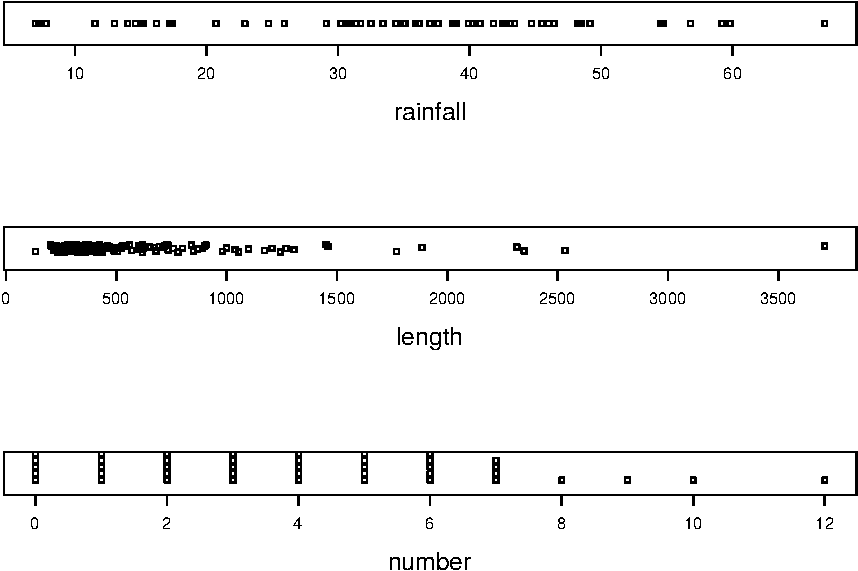
\includegraphics{_main_files/figure-latex/stripcharts-1.pdf}
\caption{\label{fig:stripcharts}\small Three stripcharts of three data sets. The
first graph uses the \texttt{overplot} method, the second the
\texttt{jitter} method, and the third the \texttt{stack} method.}
\end{figure}





The \texttt{DOTplot} \index{DOTplot@\texttt{DOTplot}} function in the
\texttt{UsingR} \index{R packages!UsingR@\texttt{UsingR}} package
\autocite{UsingR} is another alternative.

\subsubsection{\texorpdfstring{Histogram
\index{Histogram}}{Histogram }}\label{histogram}

These are typically used for continuous data. A histogram is constructed
by first deciding on a set of classes, or bins, which partition the real
line into a set of boxes into which the data values fall. Then vertical
bars are drawn over the bins with height proportional to the number of
observations that fell into the bin.

These are one of the most common summary displays, and they are often
misidentified as ``Bar Graphs'' (see below.) The scale on the \(y\) axis
can be frequency, percentage, or density (relative frequency). The term
histogram was coined by Karl Pearson in 1891, see \autocite{Miller}.

\bigskip

\BeginKnitrBlock{example}[Annual Precipitation in US Cities]
\protect\hypertarget{ex:annual}{}{\label{ex:annual} \iffalse (Annual
Precipitation in US Cities) \fi }We are going to take another look at
the \texttt{precip} \index{Data sets!precip@\texttt{precip}} data that
we investigated earlier. The strip chart in Figure \ref{fig:stripcharts}
suggested a loosely balanced distribution; let us now look to see what a
histogram says.
\EndKnitrBlock{example}

There are many ways to plot histograms in R, and one of the easiest is
with the \texttt{hist} \index{hist@\texttt{hist}} function. The
following code produces the plots in Figure \ref{fig-histograms}.

\begin{Shaded}
\begin{Highlighting}[]
\KeywordTok{hist}\NormalTok{(precip, }\DataTypeTok{main =} \StringTok{""}\NormalTok{)}
\KeywordTok{hist}\NormalTok{(precip, }\DataTypeTok{freq =} \OtherTok{FALSE}\NormalTok{, }\DataTypeTok{main =} \StringTok{""}\NormalTok{)}
\end{Highlighting}
\end{Shaded}

Notice the argument \(\mathtt{main = ""}\) which suppresses the main
title from being displayed -- it would have said ``Histogram of
\texttt{precip}'' otherwise. The plot on the left is a frequency
histogram (the default), and the plot on the right is a relative
frequency histogram (\texttt{freq\ =\ FALSE}).

\begin{figure}[htbp]
\centering
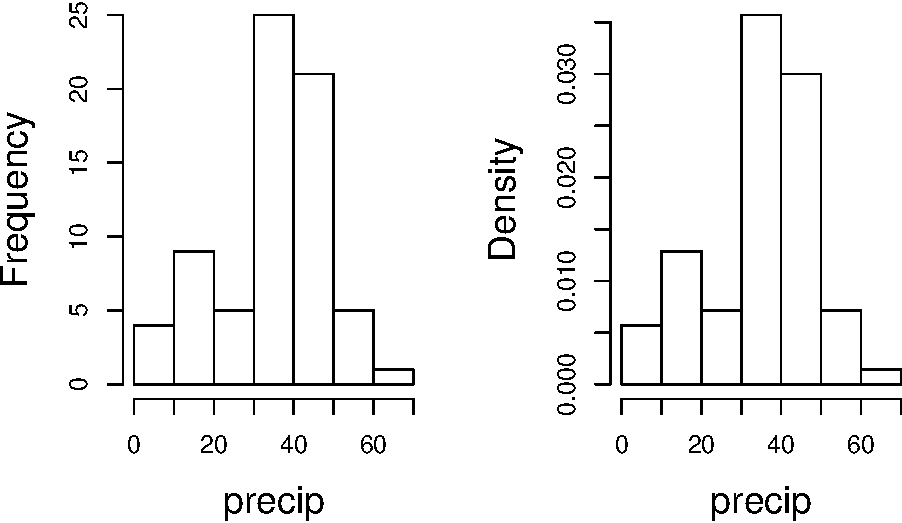
\includegraphics{_main_files/figure-latex/histograms-1.pdf}
\caption{\label{fig:histograms}\small (Relative) frequency histograms of the
\texttt{precip} data.}
\end{figure}




Please mind the biggest weakness of histograms: the graph obtained
strongly depends on the bins chosen. Choose another set of bins, and you
will get a different histogram. Moreover, there are not any definitive
criteria by which bins should be defined; the best choice for a given
data set is the one which illuminates the data set's underlying
structure (if any). Luckily for us there are algorithms to automatically
choose bins that are likely to display well, and more often than not the
default bins do a good job. This is not always the case, however, and a
responsible statistician will investigate many bin choices to test the
stability of the display.

Recall that the strip chart in Figure \ref{fig:stripcharts} suggested a
relatively balanced shape to the \texttt{precip} data distribution.
Watch what happens when we change the bins slightly (with the
\texttt{breaks} argument to \texttt{hist}). See Figure
\ref{fig:histograms-bins} which was produced by the following code.

\begin{Shaded}
\begin{Highlighting}[]
\KeywordTok{hist}\NormalTok{(precip, }\DataTypeTok{breaks =} \DecValTok{10}\NormalTok{)}
\KeywordTok{hist}\NormalTok{(precip, }\DataTypeTok{breaks =} \DecValTok{25}\NormalTok{)}
\KeywordTok{hist}\NormalTok{(precip, }\DataTypeTok{breaks =} \DecValTok{50}\NormalTok{)}
\end{Highlighting}
\end{Shaded}

\begin{figure}[htbp]
\centering
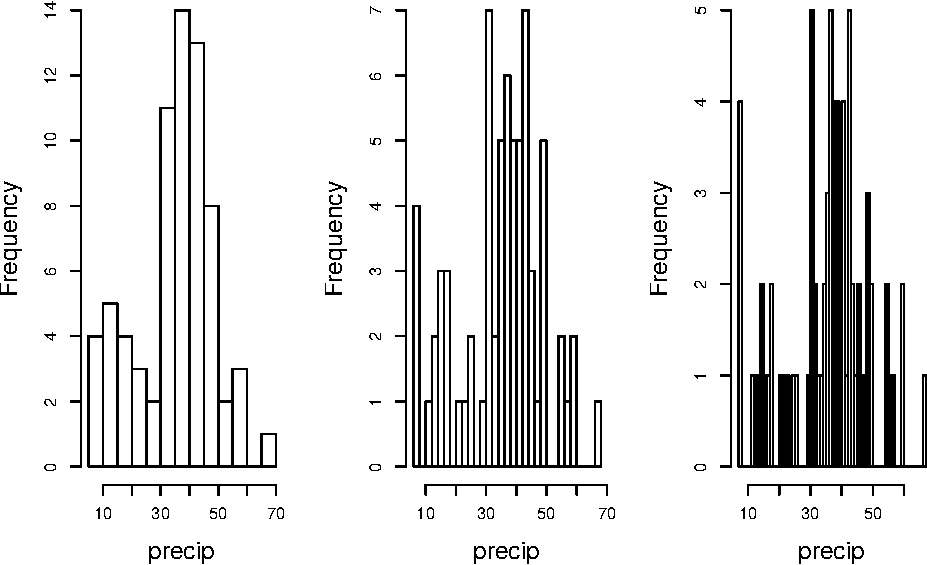
\includegraphics{_main_files/figure-latex/histograms-bins-1.pdf}
\caption{\label{fig:histograms-bins}\small More histograms of the \texttt{precip}
data.}
\end{figure}




The leftmost graph (with \texttt{breaks\ =\ 10}) shows that the
distribution is not balanced at all. There are two humps: a big one in
the middle and a smaller one to the left. Graphs like this often
indicate some underlying group structure to the data; we could now
investigate whether the cities for which rainfall was measured were
similar in some way, with respect to geographic region, for example.

The rightmost graph in Figure \ref{fig:histograms-bins} shows what
happens when the number of bins is too large: the histogram is too
grainy and hides the rounded appearance of the earlier histograms. If we
were to continue increasing the number of bins we would eventually get
all observed bins to have exactly one element, which is nothing more
than a glorified strip chart.

\subsubsection{Stem-and-leaf displays (more to be said in Section
\ref{sec-exploratory-data-analysis})}\label{stem-and-leaf-displays-more-to-be-said-in-section-refsec-exploratory-data-analysis}

Stem-and-leaf displays (also known as stemplots) have two basic parts:
\emph{stems} and \emph{leaves}. The final digit of the data values is
taken to be a \emph{leaf}, and the leading digit(s) is (are) taken to be
\emph{stems}. We draw a vertical line, and to the left of the line we
list the stems. To the right of the line, we list the leaves beside
their corresponding stem. There will typically be several leaves for
each stem, in which case the leaves accumulate to the right. It is
sometimes necessary to round the data values, especially for larger data
sets.

\bigskip

\BeginKnitrBlock{example}[Driver Deaths in the United Kingdom]
\protect\hypertarget{ex:ukdriverdeaths-first}{}{\label{ex:ukdriverdeaths-first}
\iffalse (Driver Deaths in the United Kingdom)
\fi }\texttt{UKDriverDeaths} \index{Data
sets!UKDriverDeaths@\texttt{UKDriverDeaths}} is a time series that
contains the total car drivers killed or seriously injured in Great
Britain monthly from Jan 1969 to Dec 1984. See \texttt{?UKDriverDeaths}.
Compulsory seat belt use was introduced on January 31, 1983. We
construct a stem and leaf diagram in R with the \texttt{stem.leaf}
\index{stem.leaf@\texttt{stem.leaf}} function from the \texttt{aplpack}
\index{R packages@\textsf{R}
packages!aplpack@\texttt{aplpack}} package \autocite{aplpack}.
\EndKnitrBlock{example}

\begin{Shaded}
\begin{Highlighting}[]
\KeywordTok{stem.leaf}\NormalTok{(UKDriverDeaths, }\DataTypeTok{depth =} \OtherTok{FALSE}\NormalTok{)}
\end{Highlighting}
\end{Shaded}

\begin{verbatim}
1 | 2: represents 120
 leaf unit: 10
            n: 192
   10 | 57
   11 | 136678
   12 | 123889
   13 | 0255666888899
   14 | 00001222344444555556667788889
   15 | 0000111112222223444455555566677779
   16 | 01222333444445555555678888889
   17 | 11233344566667799
   18 | 00011235568
   19 | 01234455667799
   20 | 0000113557788899
   21 | 145599
   22 | 013467
   23 | 9
   24 | 7
HI: 2654
\end{verbatim}

The display shows a more or less balanced mound-shaped distribution,
with one or maybe two humps, a big one and a smaller one just to its
right. Note that the data have been rounded to the tens place so that
each datum gets only one leaf to the right of the dividing line.

Notice that the \texttt{depth}s \index{depths} have been suppressed. To
learn more about this option and many others, see Section
\ref{sec-exploratory-data-analysis}. Unlike a histogram, the original
data values may be recovered from the stem-and-leaf display -- modulo
the rounding -- that is, starting from the top and working down we can
read off the data values 1050, 1070, 1110, 1130, and so forth.

\subsubsection{Index plots}\label{index-plots}

Done with the \texttt{plot} \index{plot@\texttt{plot}} function. These
are good for plotting data which are ordered, for example, when the data
are measured over time. That is, the first observation was measured at
time 1, the second at time 2, \emph{etc}. It is a two dimensional plot,
in which the index (or time) is the \(x\) variable and the measured
value is the \(y\) variable. There are several plotting methods for
index plots, and we mention two of them:

\begin{itemize}
\tightlist
\item
  \texttt{spikes}: draws a vertical line from the \(x\)-axis to the
  observation height.
\item
  \texttt{points}: plots a simple point at the observation height.
\end{itemize}

\bigskip

\BeginKnitrBlock{example}[Level of Lake Huron 1875-1972]
\protect\hypertarget{ex:unnamed-chunk-36}{}{\label{ex:unnamed-chunk-36}
\iffalse (Level of Lake Huron 1875-1972) \fi }Brockwell and Davis
\autocite{Brockwell1991} give the annual measurements of the level (in
feet) of Lake Huron from 1875--1972. The data are stored in the time
series \texttt{LakeHuron}. \index{Data
sets!LakeHuron@\texttt{LakeHuron}} See \texttt{?LakeHuron}. Figure
\ref{fig-indpl-lakehuron} was produced with the following code:
\EndKnitrBlock{example}

\begin{Shaded}
\begin{Highlighting}[]
\KeywordTok{plot}\NormalTok{(LakeHuron)}
\KeywordTok{plot}\NormalTok{(LakeHuron, }\DataTypeTok{type =} \StringTok{"p"}\NormalTok{)}
\KeywordTok{plot}\NormalTok{(LakeHuron, }\DataTypeTok{type =} \StringTok{"h"}\NormalTok{)}
\end{Highlighting}
\end{Shaded}

The plots show an overall decreasing trend to the observations, and
there appears to be some seasonal variation that increases over time.

\begin{figure}[htbp]
\centering
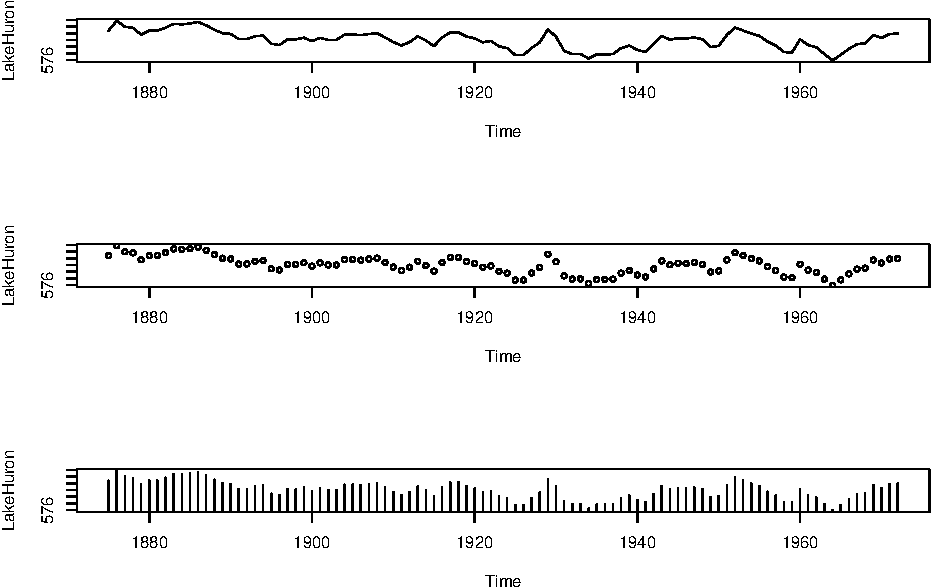
\includegraphics{_main_files/figure-latex/unnamed-chunk-38-1.pdf}
\caption{\label{fig:unnamed-chunk-38}\small Index plots of the \texttt{LakeHuron} data.}
\end{figure}



\subsubsection{Density estimates}\label{density-estimates}

The default method uses a Gaussian kernel density estimate.

\begin{Shaded}
\begin{Highlighting}[]
\CommentTok{# The Old Faithful geyser data}
\NormalTok{d <-}\StringTok{ }\KeywordTok{density}\NormalTok{(faithful$eruptions, }\DataTypeTok{bw =} \StringTok{"sj"}\NormalTok{)}
\NormalTok{d}
\KeywordTok{plot}\NormalTok{(d)}
\KeywordTok{hist}\NormalTok{(precip, }\DataTypeTok{freq =} \OtherTok{FALSE}\NormalTok{)}
\KeywordTok{lines}\NormalTok{(}\KeywordTok{density}\NormalTok{(precip))}
\end{Highlighting}
\end{Shaded}

\subsection{Qualitative Data, Categorical Data, and
Factors}\label{sub-qualitative-data}

Qualitative data are simply any type of data that are not numerical, or
do not represent numerical quantities. Examples of qualitative variables
include a subject's name, gender, race/ethnicity, political party,
socioeconomic status, class rank, driver's license number, and social
security number (SSN).

Please bear in mind that some data \emph{look} to be quantitative but
are \emph{not}, because they do not represent numerical quantities and
do not obey mathematical rules. For example, a person's shoe size is
typically written with numbers: 8, or 9, or 12, or \(12\,\frac{1}{2}\).
Shoe size is not quantitative, however, because if we take a size 8 and
combine with a size 9 we do not get a size 17.

Some qualitative data serve merely to \emph{identify} the observation
(such a subject's name, driver's license number, or SSN). This type of
data does not usually play much of a role in statistics. But other
qualitative variables serve to \emph{subdivide} the data set into
categories; we call these \emph{factors}. In the above examples, gender,
race, political party, and socioeconomic status would be considered
factors (shoe size would be another one). The possible values of a
factor are called its \emph{levels}. For instance, the factor of gender
would have two levels, namely, male and female. Socioeconomic status
typically has three levels: high, middle, and low.

Factors may be of two types: \emph{nominal} \index{nominal data} and
\emph{ordinal}. \index{ordinal data} Nominal factors have levels that
correspond to names of the categories, with no implied ordering.
Examples of nominal factors would be hair color, gender, race, or
political party. There is no natural ordering to ``Democrat'' and
``Republican''; the categories are just names associated with different
groups of people.

In contrast, ordinal factors have some sort of ordered structure to the
underlying factor levels. For instance, socioeconomic status would be an
ordinal categorical variable because the levels correspond to ranks
associated with income, education, and occupation. Another example of
ordinal categorical data would be class rank.

Factors have special status in R. They are represented internally by
numbers, but even when they are written numerically their values do not
convey any numeric meaning or obey any mathematical rules (that is,
Stage III cancer is not Stage I cancer + Stage II cancer).

\bigskip

\BeginKnitrBlock{example}
\protect\hypertarget{ex:unnamed-chunk-40}{}{\label{ex:unnamed-chunk-40}}The
\texttt{state.abb} \index{Data sets!state.abb@\texttt{state.abb}} vector
gives the two letter postal abbreviations for all 50 states.
\EndKnitrBlock{example}

\begin{Shaded}
\begin{Highlighting}[]
\KeywordTok{str}\NormalTok{(state.abb)}
\end{Highlighting}
\end{Shaded}

\begin{verbatim}
 chr [1:50] "AL" "AK" "AZ" "AR" "CA" "CO" ...
\end{verbatim}

These would be ID data. The \texttt{state.name} \index{Data
sets!state.name@\texttt{state.name}} vector lists all of the complete
names and those data would also be ID.

\bigskip

\BeginKnitrBlock{example}[U.S. State Facts and Features]
\protect\hypertarget{ex:unnamed-chunk-42}{}{\label{ex:unnamed-chunk-42}
\iffalse (U.S. State Facts and Features) \fi }The U.S. Department of
Commerce of the U.S. Census Bureau releases all sorts of information in
the \emph{Statistical Abstract of the United States}, and the
\texttt{state.region} \index{Data
sets!state.region@\texttt{state.region}} data lists each of the 50
states and the region to which it belongs, be it Northeast, South, North
Central, or West. See \texttt{?state.region}.
\EndKnitrBlock{example}

\begin{Shaded}
\begin{Highlighting}[]
\KeywordTok{str}\NormalTok{(state.region)}
\end{Highlighting}
\end{Shaded}

\begin{verbatim}
 Factor w/ 4 levels "Northeast","South",..: 2 4 4 2 4 4 1 2 2 2 ...
\end{verbatim}

\begin{Shaded}
\begin{Highlighting}[]
\NormalTok{state.region[}\DecValTok{1}\NormalTok{:}\DecValTok{5}\NormalTok{]}
\end{Highlighting}
\end{Shaded}

\begin{verbatim}
[1] South West  West  South West 
Levels: Northeast South North Central West
\end{verbatim}

The \texttt{str} \index{str@\texttt{str}} output shows that
\texttt{state.region} is already stored internally as a factor and it
lists a couple of the factor levels. To see all of the levels we printed
the first five entries of the vector in the second line.

\subsection{Displaying Qualitative
Data}\label{sub-displaying-qualitative-data}

\subsubsection{Tables}\label{par-tables}

One of the best ways to summarize qualitative data is with a table of
the data values. We may count frequencies with the \texttt{table}
function or list proportions with the \texttt{prop.table}
\index{prop.table@\texttt{prop.table}} function (whose input is a
frequency table). In the R Commander you can do it with
\texttt{Statistics} \(\triangleright\)
\texttt{Frequency\ Distribution...} Alternatively, to look at tables for
all factors in the \texttt{Active\ data\ set}
\index{Active data set@\texttt{Active data set}} you can do
\texttt{Statistics} \(\triangleright\) \texttt{Summaries}
\(\triangleright\) \texttt{Active\ Dataset}.

\begin{Shaded}
\begin{Highlighting}[]
\NormalTok{Tbl <-}\StringTok{ }\KeywordTok{table}\NormalTok{(state.division)}
\NormalTok{Tbl}
\end{Highlighting}
\end{Shaded}

\begin{verbatim}
state.division
       New England    Middle Atlantic     South Atlantic 
                 6                  3                  8 
East South Central West South Central East North Central 
                 4                  4                  5 
West North Central           Mountain            Pacific 
                 7                  8                  5 
\end{verbatim}

\begin{Shaded}
\begin{Highlighting}[]
\NormalTok{Tbl/}\KeywordTok{sum}\NormalTok{(Tbl)      }\CommentTok{# relative frequencies}
\end{Highlighting}
\end{Shaded}

\begin{verbatim}
state.division
       New England    Middle Atlantic     South Atlantic 
              0.12               0.06               0.16 
East South Central West South Central East North Central 
              0.08               0.08               0.10 
West North Central           Mountain            Pacific 
              0.14               0.16               0.10 
\end{verbatim}

\begin{Shaded}
\begin{Highlighting}[]
\KeywordTok{prop.table}\NormalTok{(Tbl)   }\CommentTok{# same thing}
\end{Highlighting}
\end{Shaded}

\begin{verbatim}
state.division
       New England    Middle Atlantic     South Atlantic 
              0.12               0.06               0.16 
East South Central West South Central East North Central 
              0.08               0.08               0.10 
West North Central           Mountain            Pacific 
              0.14               0.16               0.10 
\end{verbatim}

\subsubsection{Bar Graphs}\label{par-bar-graphs}

A bar graph is the analogue of a histogram for categorical data. A bar
is displayed for each level of a factor, with the heights of the bars
proportional to the frequencies of observations falling in the
respective categories. A disadvantage of bar graphs is that the levels
are ordered alphabetically (by default), which may sometimes obscure
patterns in the display.

\bigskip

\BeginKnitrBlock{example}[U.S. State Facts and Features]
\protect\hypertarget{ex:unnamed-chunk-47}{}{\label{ex:unnamed-chunk-47}
\iffalse (U.S. State Facts and Features) \fi }The \texttt{state.region}
data lists each of the 50 states and the region to which it belongs, be
it Northeast, South, North Central, or West. See \texttt{?state.region}.
It is already stored internally as a factor. We make a bar graph with
the \texttt{barplot} \index{barplot@\texttt{barplot}} function:
\EndKnitrBlock{example}

\begin{Shaded}
\begin{Highlighting}[]
\KeywordTok{barplot}\NormalTok{(}\KeywordTok{table}\NormalTok{(state.region), }\DataTypeTok{cex.names =} \FloatTok{1.20}\NormalTok{)}
\KeywordTok{barplot}\NormalTok{(}\KeywordTok{prop.table}\NormalTok{(}\KeywordTok{table}\NormalTok{(state.region)), }\DataTypeTok{cex.names =} \FloatTok{1.20}\NormalTok{)}
\end{Highlighting}
\end{Shaded}

See Figure \ref{fig:bar-gr-stateregion}. The display on the left is a
frequency bar graph because the \(y\) axis shows counts, while the
display on the left is a relative frequency bar graph. The only
difference between the two is the scale. Looking at the graph we see
that the majority of the fifty states are in the South, followed by
West, North Central, and finally Northeast. Over 30\% of the states are
in the South.

Notice the \texttt{cex.names} \index{cex.names@\texttt{cex.names}}
argument that we used, above. It expands the names on the \(x\) axis by
20\% which makes them easier to read. See \texttt{?par}
\index{par@\texttt{par}} for a detailed list of additional plot
parameters.

\begin{figure}[htbp]
\centering
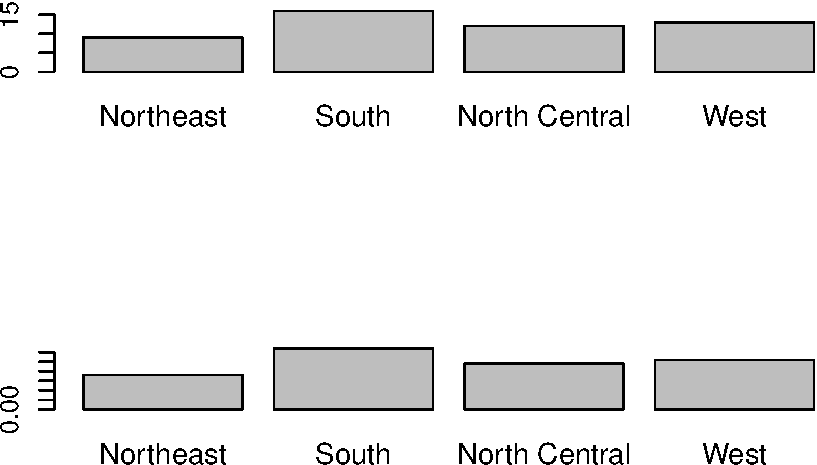
\includegraphics{_main_files/figure-latex/bar-gr-stateregion-1.pdf}
\caption{\label{fig:bar-gr-stateregion}\small The top graph is a frequency barplot made
with \texttt{table} and the bottom is a relative frequency barplot made
with \texttt{prop.table}.}
\end{figure}





\subsubsection{Pareto Diagrams}\label{par-pareto-diagrams}

A pareto diagram is a lot like a bar graph except the bars are
rearranged such that they decrease in height going from left to right.
The rearrangement is handy because it can visually reveal structure (if
any) in how fast the bars decrease -- this is much more difficult when
the bars are jumbled.

\bigskip

\BeginKnitrBlock{example}[U.S. State Facts and Features]
\protect\hypertarget{ex:unnamed-chunk-49}{}{\label{ex:unnamed-chunk-49}
\iffalse (U.S. State Facts and Features) \fi }The
\texttt{state.division} \index{Data
sets!state.division@\texttt{state.division}} data record the division
(New England, Middle Atlantic, South Atlantic, East South Central, West
South Central, East North Central, West North Central, Mountain, and
Pacific) of the fifty states. We can make a pareto diagram with either
the \texttt{RcmdrPlugin.IPSUR} \index{R
packages@\textsf{R}
packages!RcmdrPlugin.IPSUR@\texttt{RcmdrPlugin.IPSUR}} package
\autocite{RcmdrPlugin.IPSUR} or with the \texttt{pareto.chart}
\index{pareto.chart@\texttt{pareto.chart}} function from the
\texttt{qcc} \index{R packages@\textsf{R}
packages!qcc@\texttt{qcc}} package \autocite{qcc}. See Figure
\ref{fig:pareto-chart}. The code follows.
\EndKnitrBlock{example}

\begin{Shaded}
\begin{Highlighting}[]
\KeywordTok{pareto.chart}\NormalTok{(}\KeywordTok{table}\NormalTok{(state.division), }\DataTypeTok{ylab=}\StringTok{"Frequency"}\NormalTok{, }\DataTypeTok{cex.lab =} \NormalTok{cexlab)}
\end{Highlighting}
\end{Shaded}

\begin{figure}[htbp]
\centering
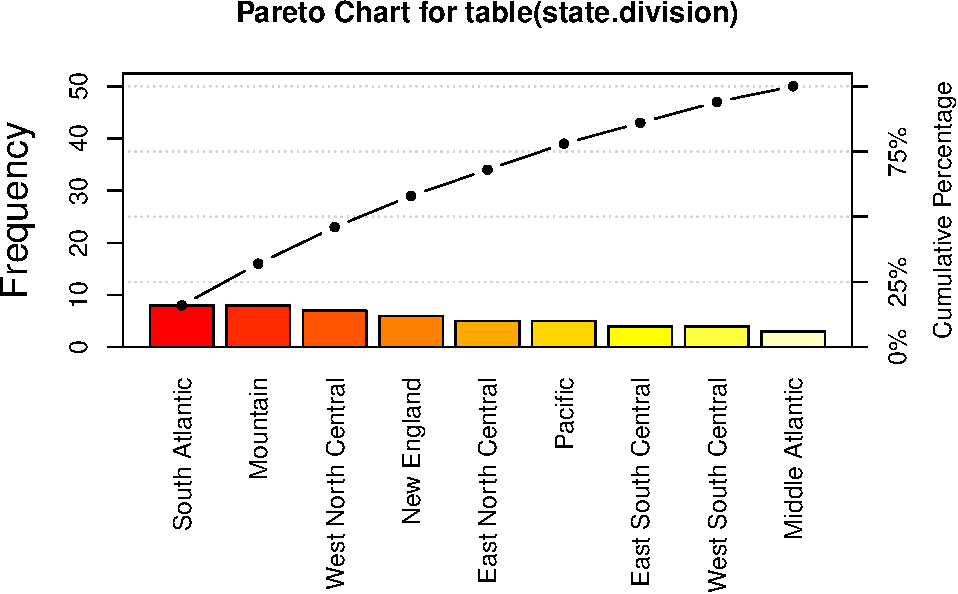
\includegraphics{_main_files/figure-latex/pareto-chart-1.pdf}
\caption{\label{fig:pareto-chart}\small Pareto chart of the \texttt{state.division}
data.}
\end{figure}

\begin{verbatim}
                    
Pareto chart analysis for table(state.division)
                     Frequency Cum.Freq. Percentage
  South Atlantic             8         8         16
  Mountain                   8        16         16
  West North Central         7        23         14
  New England                6        29         12
  East North Central         5        34         10
  Pacific                    5        39         10
  East South Central         4        43          8
  West South Central         4        47          8
  Middle Atlantic            3        50          6
                    
Pareto chart analysis for table(state.division)
                     Cum.Percent.
  South Atlantic               16
  Mountain                     32
  West North Central           46
  New England                  58
  East North Central           68
  Pacific                      78
  East South Central           86
  West South Central           94
  Middle Atlantic             100
\end{verbatim}




\subsubsection{Dot Charts}\label{par-dotcharts}

These are a lot like a bar graph that has been turned on its side with
the bars replaced by dots on horizontal lines. They do not convey any
more (or less) information than the associated bar graph, but the
strength lies in the economy of the display. Dot charts are so compact
that it is easy to graph very complicated multi-variable interactions
together in one graph. See Section \ref{sec-comparing-data-sets}. We
will give an example here using the same data as above for comparison.
The graph was produced by the following code.

\begin{Shaded}
\begin{Highlighting}[]
\NormalTok{x <-}\StringTok{ }\KeywordTok{table}\NormalTok{(state.region)}
\KeywordTok{dotchart}\NormalTok{(}\KeywordTok{as.vector}\NormalTok{(x), }\DataTypeTok{labels =} \KeywordTok{names}\NormalTok{(x), }\DataTypeTok{cex.lab =} \NormalTok{cexlab)}
\end{Highlighting}
\end{Shaded}

\begin{figure}[htbp]
\centering
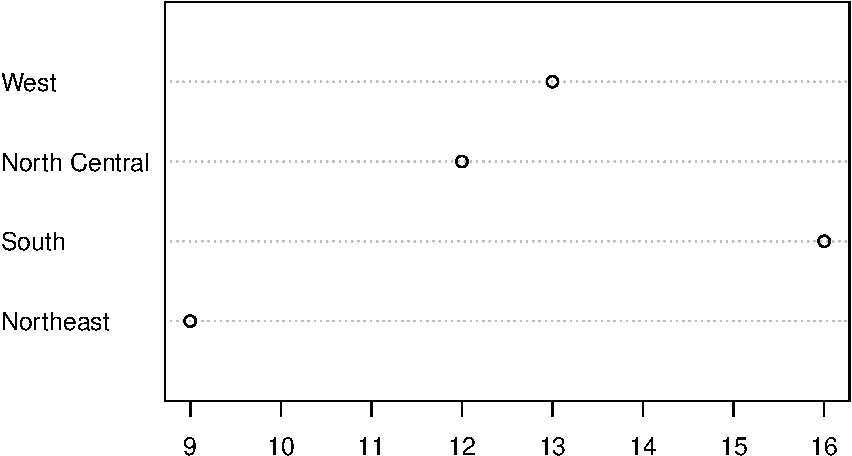
\includegraphics{_main_files/figure-latex/dotchart-1.pdf}
\caption{\label{fig:dotchart}\small Dot chart of the \texttt{state.region} data.}
\end{figure}



See Figure \ref{fig:dotchart}. Compare it to Figure
\ref{fig:bar-gr-stateregion}.

\subsubsection{Pie Graphs}\label{par-pie-graphs}

These can be done with R and the R Commander, but they fallen out of
favor in recent years because researchers have determined that while the
human eye is good at judging linear measures, it is notoriously bad at
judging relative areas (such as those displayed by a pie graph). Pie
charts are consequently a very bad way of displaying information unless
the number of categories is two or three. A bar chart or dot chart is a
preferable way of displaying qualitative data. See \texttt{?pie}
\index{pie@\texttt{pie}} for more information.

We are not going to do any examples of a pie graph and discourage their
use elsewhere.

\subsection{Logical Data}\label{sub-logical-data}

There is another type of information recognized by R which does not fall
into the above categories. The value is either \texttt{TRUE} or
\texttt{FALSE} (note that equivalently you can use \texttt{1\ =\ TRUE},
\texttt{0\ =\ FALSE}). Here is an example of a logical vector:

\begin{Shaded}
\begin{Highlighting}[]
\NormalTok{x <-}\StringTok{ }\DecValTok{5}\NormalTok{:}\DecValTok{9}
\NormalTok{y <-}\StringTok{ }\NormalTok{(x <}\StringTok{ }\FloatTok{7.3}\NormalTok{)}
\NormalTok{y}
\end{Highlighting}
\end{Shaded}

\begin{verbatim}
[1]  TRUE  TRUE  TRUE FALSE FALSE
\end{verbatim}

Many functions in R have options that the user may or may not want to
activate in the function call. For example, the \texttt{stem.leaf}
function has the \texttt{depths} argument which is \texttt{TRUE} by
default. We saw in Section \ref{sub-quantitative-data} how to turn the
option off, simply enter \texttt{stem.leaf(x,\ depths\ =\ FALSE)} and
they will not be shown on the display.

We can swap \texttt{TRUE} with \texttt{FALSE} with the exclamation point
\texttt{!}.

\begin{Shaded}
\begin{Highlighting}[]
\NormalTok{!y}
\end{Highlighting}
\end{Shaded}

\begin{verbatim}
[1] FALSE FALSE FALSE  TRUE  TRUE
\end{verbatim}

\subsection{Missing Data}\label{sub-missing-data}

Missing data are a persistent and prevalent problem in many statistical
analyses, especially those associated with the social sciences. R
reserves the special symbol \texttt{NA} to representing missing data.

Ordinary arithmetic with \texttt{NA} values give \texttt{NA}'s
(addition, subtraction, \emph{etc}.) and applying a function to a vector
that has an \texttt{NA} in it will usually give an \texttt{NA}.

\begin{Shaded}
\begin{Highlighting}[]
\NormalTok{x <-}\StringTok{ }\KeywordTok{c}\NormalTok{(}\DecValTok{3}\NormalTok{, }\DecValTok{7}\NormalTok{, }\OtherTok{NA}\NormalTok{, }\DecValTok{4}\NormalTok{, }\DecValTok{7}\NormalTok{)}
\NormalTok{y <-}\StringTok{ }\KeywordTok{c}\NormalTok{(}\DecValTok{5}\NormalTok{, }\OtherTok{NA}\NormalTok{, }\DecValTok{1}\NormalTok{, }\DecValTok{2}\NormalTok{, }\DecValTok{2}\NormalTok{)}
\NormalTok{x +}\StringTok{ }\NormalTok{y}
\end{Highlighting}
\end{Shaded}

\begin{verbatim}
[1]  8 NA NA  6  9
\end{verbatim}

Some functions have a \texttt{na.rm} argument which when \texttt{TRUE}
will ignore missing data as if they were not there (such as
\texttt{mean}, \texttt{var}, \texttt{sd}, \texttt{IQR}, \texttt{mad},
\ldots{}).

\begin{Shaded}
\begin{Highlighting}[]
\KeywordTok{sum}\NormalTok{(x)}
\end{Highlighting}
\end{Shaded}

\begin{verbatim}
[1] NA
\end{verbatim}

\begin{Shaded}
\begin{Highlighting}[]
\KeywordTok{sum}\NormalTok{(x, }\DataTypeTok{na.rm =} \OtherTok{TRUE}\NormalTok{)}
\end{Highlighting}
\end{Shaded}

\begin{verbatim}
[1] 21
\end{verbatim}

Other functions do not have a \texttt{na.rm} argument and will return
\texttt{NA} or an error if the argument has \texttt{NA}s. In those cases
we can find the locations of any \texttt{NA}s with the \texttt{is.na}
function and remove those cases with the \texttt{{[}{]}} operator.

\begin{Shaded}
\begin{Highlighting}[]
\KeywordTok{is.na}\NormalTok{(x)}
\end{Highlighting}
\end{Shaded}

\begin{verbatim}
[1] FALSE FALSE  TRUE FALSE FALSE
\end{verbatim}

\begin{Shaded}
\begin{Highlighting}[]
\NormalTok{z <-}\StringTok{ }\NormalTok{x[!}\KeywordTok{is.na}\NormalTok{(x)]}
\KeywordTok{sum}\NormalTok{(z)}
\end{Highlighting}
\end{Shaded}

\begin{verbatim}
[1] 21
\end{verbatim}

The analogue of \texttt{is.na} for rectangular data sets (or data
frames) is the \texttt{complete.cases} function. See Appendix
\ref{sec-editing-data-sets}.

\subsection{Other Data Types}\label{sub-other-data-types}

\section{Features of Data Distributions}\label{sec-features-of-data}

Given that the data have been appropriately displayed, the next step is
to try to identify salient features represented in the graph. The
acronym to remember is \emph{C}-enter, \emph{U}-nusual features,
\emph{S}-pread, and \emph{S}-hape. (CUSS).

\subsection{Center}\label{sub-center}

One of the most basic features of a data set is its center. Loosely
speaking, the center of a data set is associated with a number that
represents a middle or general tendency of the data. Of course, there
are usually several values that would serve as a center, and our later
tasks will be focused on choosing an appropriate one for the data at
hand. Judging from the histogram that we saw in Figure
\ref{fig:histograms-bins}, a measure of center would be about 35.

\subsection{Spread}\label{sub-spread}

The spread of a data set is associated with its variability; data sets
with a large spread tend to cover a large interval of values, while data
sets with small spread tend to cluster tightly around a central value.

\subsection{Shape}\label{sub-shape}

When we speak of the \emph{shape} of a data set, we are usually
referring to the shape exhibited by an associated graphical display,
such as a histogram. The shape can tell us a lot about any underlying
structure to the data, and can help us decide which statistical
procedure we should use to analyze them.

\subsubsection{Symmetry and Skewness}\label{symmetry-and-skewness}

A distribution is said to be \emph{right-skewed} (or \emph{positively
skewed}) if the right tail seems to be stretched from the center. A
\emph{left-skewed} (or \emph{negatively skewed}) distribution is
stretched to the left side. A symmetric distribution has a graph that is
balanced about its center, in the sense that half of the graph may be
reflected about a central line of symmetry to match the other half.

We have already encountered skewed distributions: both the discoveries
data in Figure \ref{fig:stripcharts} and the \texttt{precip} data in
Figure \ref{fig:histograms-bins} appear right-skewed. The
\texttt{UKDriverDeaths} data in Example \ref{ex:ukdriverdeaths-first} is
relatively symmetric (but note the one extreme value 2654 identified at
the bottom of the stem-and-leaf display).

\subsubsection{Kurtosis}\label{kurtosis}

Another component to the shape of a distribution is how ``peaked'' it
is. Some distributions tend to have a flat shape with thin tails. These
are called \emph{platykurtic}, and an example of a platykurtic
distribution is the uniform distribution; see Section
\ref{sec-the-continuous-uniform}. On the other end of the spectrum are
distributions with a steep peak, or spike, accompanied by heavy tails;
these are called \emph{leptokurtic}. Examples of leptokurtic
distributions are the Laplace distribution and the logistic
distribution. See Section \ref{sec-other-continuous-distributions}. In
between are distributions (called \emph{mesokurtic}) with a rounded peak
and moderately sized tails. The standard example of a mesokurtic
distribution is the famous bell-shaped curve, also known as the
Gaussian, or normal, distribution, and the binomial distribution can be
mesokurtic for specific choices of \(p\). See Sections
\ref{sec-binom-dist} and \ref{sec-the-normal-distribution}.

\subsection{Clusters and Gaps}\label{sub-clusters-and-gaps}

Clusters or gaps are sometimes observed in quantitative data
distributions. They indicate clumping of the data about distinct values,
and gaps may exist between clusters. Clusters often suggest an
underlying grouping to the data. For example, take a look at the
\texttt{faithful} data which contains the duration of \texttt{eruptions}
and the \texttt{waiting} time between eruptions of the Old Faithful
geyser in Yellowstone National Park. Do not be frightened by the
complicated information at the left of the display for now; we will
learn how to interpret it in Section
\ref{sec-exploratory-data-analysis}.

\begin{Shaded}
\begin{Highlighting}[]
\KeywordTok{with}\NormalTok{(faithful, }\KeywordTok{stem.leaf}\NormalTok{(eruptions))}
\end{Highlighting}
\end{Shaded}

\begin{verbatim}
1 | 2: represents 1.2
 leaf unit: 0.1
            n: 272
   12     s | 667777777777
   51    1. | 888888888888888888888888888899999999999
   71    2* | 00000000000011111111
   87     t | 2222222222333333
   92     f | 44444
   94     s | 66
   97    2. | 889
   98    3* | 0
  102     t | 3333
  108     f | 445555
  118     s | 6666677777
  (16)   3. | 8888888889999999
  138    4* | 0000000000000000111111111111111
  107     t | 22222222222233333333333333333
   78     f | 44444444444445555555555555555555555
   43     s | 6666666666677777777777
   21    4. | 88888888888899999
    4    5* | 0001
\end{verbatim}

There are definitely two clusters of data here; an upper cluster and a
lower cluster.

\subsection{Extreme Observations and other Unusual
Features}\label{sub-extreme-observations}

Extreme observations fall far from the rest of the data. Such
observations are troublesome to many statistical procedures; they cause
exaggerated estimates and instability. It is important to identify
extreme observations and examine the source of the data more closely.
There are many possible reasons underlying an extreme observation:

\begin{itemize}
\tightlist
\item
  \emph{Maybe the value is a typographical error.} Especially with large
  data sets becoming more prevalent, many of which being recorded by
  hand, mistakes are a common problem. After closer scrutiny, these can
  often be fixed.
\item
  \emph{Maybe the observation was not meant for the study}, because it
  does not belong to the population of interest. For example, in medical
  research some subjects may have relevant complications in their
  genealogical history that would rule out their participation in the
  experiment. Or when a manufacturing company investigates the
  properties of one of its devices, perhaps a particular product is
  malfunctioning and is not representative of the majority of the items.
\item
  \emph{Maybe it indicates a deeper trend or phenomenon.} Many of the
  most influential scientific discoveries were made when the
  investigator noticed an unexpected result, a value that was not
  predicted by the classical theory. Albert Einstein, Louis Pasteur, and
  others built their careers on exactly this circumstance.
\end{itemize}

\section{Descriptive Statistics}\label{sec-descriptive-statistics}

One of my favorite professors would repeatedly harp, ``You cannot do
statistics without data.''

\textbf{What do I want them to know?}

\begin{itemize}
\tightlist
\item
  The fundamental data types we encounter most often, how to classify
  given data into a likely type, and that sometimes the distinction is
  blurry.
\end{itemize}

\subsection{Frequencies and Relative
Frequencies}\label{sub-frequencies-and-relative}

These are used for categorical data. The idea is that there are a number
of different categories, and we would like to get some idea about how
the categories are represented in the population.

\subsection{Measures of Center}\label{sub-measures-of-center}

The \emph{sample mean} is denoted \(\overline{x}\) (read ``\(x\)-bar'')
and is simply the arithmetic average of the observations:

\begin{equation} 
\overline{x}=\frac{x_{1}+x_{2}+\cdots+x_{n}}{n}=\frac{1}{n}\sum_{i=1}^{n}x_{i}.
\end{equation}

\begin{itemize}
\tightlist
\item
  Good: natural, easy to compute, has nice mathematical properties
\item
  Bad: sensitive to extreme values
\end{itemize}

It is appropriate for use with data sets that are not highly skewed
without extreme observations.

The \emph{sample median} is another popular measure of center and is
denoted \(\tilde{x}\). To calculate its value, first sort the data into
an increasing sequence of numbers. If the data set has an odd number of
observations then \(\tilde{x}\) is the value of the middle observation,
which lies in position \((n+1)/2\); otherwise, there are two middle
observations and \(\tilde{x}\) is the average of those middle values.

\begin{itemize}
\tightlist
\item
  Good: resistant to extreme values, easy to describe
\item
  Bad: not as mathematically tractable, need to sort the data to
  calculate
\end{itemize}

One desirable property of the sample median is that it is
\emph{resistant} to extreme observations, in the sense that the value of
\(\tilde{x}\) depends only on those data values in the middle, and is
quite unaffected by the actual values of the outer observations in the
ordered list. The same cannot be said for the sample mean. Any
significant changes in the magnitude of an observation \(x_{k}\) results
in a corresponding change in the value of the mean. Consequently, the
sample mean is said to be \emph{sensitive} to extreme observations.

The \emph{trimmed mean} is a measure designed to address the sensitivity
of the sample mean to extreme observations. The idea is to ``trim'' a
fraction (less than 1/2) of the observations off each end of the ordered
list, and then calculate the sample mean of what remains. We will denote
it by \(\overline{x}_{t=0.05}\).

\begin{itemize}
\tightlist
\item
  Good: resistant to extreme values, shares nice statistical properties
\item
  Bad: need to sort the data
\end{itemize}

\subsubsection{How to do it with R}\label{how-to-do-it-with-r}

\begin{itemize}
\tightlist
\item
  You can calculate frequencies or relative frequencies with the
  \texttt{table} function, and relative frequencies with
  \texttt{prop.table(table())}.
\item
  You can calculate the sample mean of a data vector \texttt{x} with the
  command \texttt{mean(x)}.
\item
  You can calculate the sample median of \texttt{x} with the command
  \texttt{median(x)}.
\item
  You can calculate the trimmed mean with the \texttt{trim} argument;
  \texttt{mean(x,\ trim\ =\ 0.05)}.
\end{itemize}

\subsection{Order Statistics and the Sample
Quantiles}\label{sub-order-statistics}

A common first step in an analysis of a data set is to sort the values.
Given a data set \(x_{1}\), \(x_{2}\), \ldots{}, \(x_{n}\), we may sort
the values to obtain an increasing sequence

\begin{equation} 
x_{(1)}\leq x_{(2)}\leq x_{(3)}\leq\cdots\leq x_{(n)}
\end{equation}

and the resulting values are called the \emph{order statistics}. The
\(k^{\mathrm{th}}\) entry in the list, \(x_{(k)}\), is the
\(k^{\mathrm{th}}\) order statistic, and approximately \(100(k/n)\)\% of
the observations fall below \(x_{(k)}\). The order statistics give an
indication of the shape of the data distribution, in the sense that a
person can look at the order statistics and have an idea about where the
data are concentrated, and where they are sparse.

The \emph{sample quantiles} are related to the order statistics.
Unfortunately, there is not a universally accepted definition of them.
Indeed, R is equipped to calculate quantiles using nine distinct
definitions! We will describe the default method (\texttt{type\ =\ 7}),
but the interested reader can see the details for the other methods with
\texttt{?quantile}.

Suppose the data set has \(n\) observations. Find the sample quantile of
order \(p\) (\(0<p<1\)), denoted \(\tilde{q}_{p}\) , as follows:

\begin{itemize}
\tightlist
\item
  \textbf{First step:} sort the data to obtain the order statistics
  \(x_{(1)}\), \(x_{(2)}\), \ldots{},\(x_{(n)}\).
\item
  \textbf{Second step:} calculate \((n-1)p+1\) and write it in the form
  \(k.d\), where \(k\) is an integer and \(d\) is a decimal.
\item
  \textbf{Third step:} The sample quantile \(\tilde{q}_{p}\) is

  \begin{equation}
    \tilde{q}_{p}=x_{(k)}+d(x_{(k+1)}-x_{(k)}).
     \end{equation}
\end{itemize}

The interpretation of \(\tilde{q}_{p}\) is that approximately \(100p\)
\% of the data fall below the value \(\tilde{q}_{p}\).

Keep in mind that there is not a unique definition of percentiles,
quartiles, \emph{etc}. Open a different book, and you'll find a
different definition. The difference is small and seldom plays a role
except in small data sets with repeated values. In fact, most people do
not even notice in common use.

Clearly, the most popular sample quantile is \(\tilde{q}_{0.50}\), also
known as the sample median, \(\tilde{x}\). The closest runners-up are
the \emph{first quartile} \(\tilde{q}_{0.25}\) and the \emph{third
quartile} \(\tilde{q}_{0.75}\) (the \emph{second quartile} is the
median).

\subsubsection{How to do it with R}\label{how-to-do-it-with-r-1}

\textbf{At the command prompt} We can find the order statistics of a
data set stored in a vector \texttt{x} with the command
\texttt{sort(x)}.

We can calculate the sample quantiles of any order \(p\) where \(0<p<1\)
for a data set stored in a data vector \texttt{x} with the
\texttt{quantile} function, for instance, the command
\texttt{quantile(x,\ probs\ =\ c(0,\ 0.25,\ 0.37))} will return the
smallest observation, the first quartile, \(\tilde{q}_{0.25}\), and the
37th sample quantile, \(\tilde{q}_{0.37}\). For \(\tilde{q}_{p}\) simply
change the values in the \texttt{probs} argument to the value \(p\).

\textbf{With the R Commander} we can find the order statistics of a
variable in the \texttt{Active\ data\ set} by doing \texttt{Data}
\(\triangleright\) \texttt{Manage\ variables\ in\ Active\ data\ set...}
\(\triangleright\) \texttt{Compute\ new\ variable...} In the
\texttt{Expression\ to\ compute} dialog simply type
\texttt{sort(varname)}, where \texttt{varname} is the variable that it
is desired to sort.

In \texttt{Rcmdr}, we can calculate the sample quantiles for a
particular variable with the sequence \texttt{Statistics}
\(\triangleright\) \texttt{Summaries} \(\triangleright\)
\texttt{Numerical\ Summaries...} We can automatically calculate the
quartiles for all variables in the \texttt{Active\ data\ set} with the
sequence \texttt{Statistics} \(\triangleright\) \texttt{Summaries}
\(\triangleright\) \texttt{Active\ Dataset}.

\subsection{Measures of Spread}\label{sub-measures-of-spread}

\subsubsection{Sample Variance and Standard
Deviation}\label{sample-variance-and-standard-deviation}

The \emph{sample variance} is denoted \(s^{2}\) and is calculated with
the formula

\begin{equation}
s^{2}=\frac{1}{n-1}\sum_{i=1}^{n}(x_{i}-\overline{x})^{2}.
\end{equation}

The \emph{sample standard deviation} is \(s=\sqrt{s^{2}}\). Intuitively,
the sample variance is approximately the average squared distance of the
observations from the sample mean. The sample standard deviation is used
to scale the estimate back to the measurement units of the original
data.

\begin{itemize}
\tightlist
\item
  Good: tractable, has nice mathematical/statistical properties
\item
  Bad: sensitive to extreme values
\end{itemize}

We will spend a lot of time with the variance and standard deviation in
the coming chapters. In the meantime, the following two rules give some
meaning to the standard deviation, in that there are bounds on how much
of the data can fall past a certain distance from the mean.

\textbf{Fact:} (Chebychev's Rule). The proportion of observations within
\(k\) standard deviations of the mean is at least \(1-1/k^{2}\),
\emph{i.e.}, at least 75\%, 89\%, and 94\% of the data are within 2, 3,
and 4 standard deviations of the mean, respectively.

Note that Chebychev's Rule does not say anything about when \(k=1\),
because \(1-1/1^{2}=0\), which states that at least 0\% of the
observations are within one standard deviation of the mean (which is not
saying much).

Chebychev's Rule applies to any data distribution, \emph{any} list of
numbers, no matter where it came from or what the histogram looks like.
The price for such generality is that the bounds are not very tight; if
we know more about how the data are shaped then we can say more about
how much of the data can fall a given distance from the mean.

\textbf{Fact:} (Empirical Rule). If data follow a bell-shaped curve,
then approximately 68\%, 95\%, and 99.7\% of the data are within 1, 2,
and 3 standard deviations of the mean, respectively.

\subsubsection{Interquartile Range}\label{interquartile-range}

Just as the sample mean is sensitive to extreme values, so the
associated measure of spread is similarly sensitive to extremes.
Further, the problem is exacerbated by the fact that the extreme
distances are squared. We know that the sample quartiles are resistant
to extremes, and a measure of spread associated with them is the
\emph{interquartile range} (\(IQR\)) defined by
\(IQR=q_{0.75}-q_{0.25}\).

\begin{itemize}
\tightlist
\item
  Good: stable, resistant to outliers, robust to nonnormality, easy to
  explain
\item
  Bad: not as tractable, need to sort the data, only involves the middle
  50\% of the data.
\end{itemize}

\subsubsection{Median Absolute
Deviation}\label{median-absolute-deviation}

A measure even more robust than the \(IQR\) is the \emph{median absolute
deviation} (\(MAD\)). To calculate it we first get the median
\(\widetilde{x}\), next the \emph{absolute deviations}
\(|x_{1}-\tilde{x}|\), \(|x_{2}-\tilde{x}|\), \ldots{},
\(|x_{n}-\tilde{x}|\), and the \(MAD\) is proportional to the median of
those deviations:

\begin{equation}
MAD\propto\mbox{median}(|x_{1}-\tilde{x}|,\ |x_{2}-\tilde{x}|,\ldots,|x_{n}-\tilde{x}|).
\end{equation}

That is, the
\(MAD=c\cdot\mbox{median}(|x_{1}-\tilde{x}|,\ |x_{2}-\tilde{x}|,\ldots,|x_{n}-\tilde{x}|)\),
where \(c\) is a constant chosen so that the \(MAD\) has nice
properties. The value of \(c\) in R is by default \(c=1.4286\). This
value is chosen to ensure that the estimator of \(\sigma\) is correct,
on the average, under suitable sampling assumptions (see Section
\ref{sec-point-estimation}).

\begin{itemize}
\tightlist
\item
  Good: stable, very robust, even more so than the \(IQR\).
\item
  Bad: not tractable, not well known and less easy to explain.
\end{itemize}

\subsubsection{Comparing Apples to
Apples}\label{comparing-apples-to-apples}

We have seen three different measures of spread which, for a given data
set, will give three different answers. Which one should we use? It
depends on the data set. If the data are well behaved, with an
approximate bell-shaped distribution, then the sample mean and sample
standard deviation are natural choices with nice mathematical
properties. However, if the data have an unusual or skewed shape with
several extreme values, perhaps the more resistant choices among the
\(IQR\) or \(MAD\) would be more appropriate.

However, once we are looking at the three numbers it is important to
understand that the estimators are not all measuring the same quantity,
on the average. In particular, it can be shown that when the data follow
an approximately bell-shaped distribution, then on the average, the
sample standard deviation \(s\) and the \(MAD\) will be the
approximately the same value, namely, \(\sigma\), but the \(IQR\) will
be on the average 1.349 times larger than \(s\) and the \(MAD\). See
\ref{cha-sampling-distributions} for more details.

\subsubsection{How to do it with R}\label{how-to-do-it-with-r-2}

\textbf{At the command prompt} we may compute the sample range with
\texttt{range(x)} and the sample variance with \texttt{var(x)}, where
\texttt{x} is a numeric vector. The sample standard deviation is
\texttt{sqrt(var(x))} or just \texttt{sd(x)}. The \(IQR\) is
\texttt{IQR(x)} and the median absolute deviation is \texttt{mad(x)}.

\textbf{With the R Commander} we can calculate the sample standard
deviation with the \texttt{Statistics} \(\triangleright\)
\texttt{Summaries} \(\triangleright\) \texttt{Numerical\ Summaries...}
combination. R Commander does not calculate the \(IQR\) or \(MAD\) in
any of the menu selections, by default.

\subsection{Measures of Shape}\label{sub-measures-of-shape}

\subsubsection{Sample Skewness}\label{sample-skewness}

The \emph{sample skewness}, denoted by \(g_{1}\), is defined by the
formula

\begin{equation}
g_{1}=\frac{1}{n}\frac{\sum_{i=1}^{n}(x_{i}-\overline{x})^{3}}{s^{3}}.
\end{equation}

The sample skewness can be any value \(-\infty<g_{1}<\infty\). The sign
of \(g_{1}\) indicates the direction of skewness of the distribution.
Samples that have \(g_{1}>0\) indicate right-skewed distributions (or
positively skewed), and samples with \(g_{1}<0\) indicate left-skewed
distributions (or negatively skewed). Values of \(g_{1}\) near zero
indicate a symmetric distribution. These are not hard and fast rules,
however. The value of \(g_{1}\) is subject to sampling variability and
thus only provides a suggestion to the skewness of the underlying
distribution.

We still need to know how big is ``big'', that is, how do we judge
whether an observed value of \(g_{1}\) is far enough away from zero for
the data set to be considered skewed to the right or left? A good rule
of thumb is that data sets with skewness larger than \(2\sqrt{6/n}\) in
magnitude are substantially skewed, in the direction of the sign of
\(g_{1}\). See Tabachnick \& Fidell \autocite{Tabachnick2006} for
details.

\subsubsection{Sample Excess Kurtosis}\label{sample-excess-kurtosis}

The \emph{sample excess kurtosis}, denoted by \(g_{2}\), is given by the
formula

\begin{equation}
g_{2}=\frac{1}{n}\frac{\sum_{i=1}^{n}(x_{i}-\overline{x})^{4}}{s^{4}}-3.
\end{equation}

The sample excess kurtosis takes values \(-2\leq g_{2}<\infty\). The
subtraction of 3 may seem mysterious but it is done so that mound shaped
samples have values of \(g_{2}\) near zero. Samples with \(g_{2}>0\) are
called \emph{leptokurtic}, and samples with \(g_{2}<0\) are called
\emph{platykurtic}. Samples with \(g_{2}\approx0\) are called
\emph{mesokurtic}.

As a rule of thumb, if \(|g_{2}|>4\sqrt{6/n}\) then the sample excess
kurtosis is substantially different from zero in the direction of the
sign of \(g_{2}\). See Tabachnick \& Fidell \autocite{Tabachnick2006}
for details.

Notice that both the sample skewness and the sample kurtosis are
invariant with respect to location and scale, that is, the values of
\(g_{1}\) and \(g_{2}\) do not depend on the measurement units of the
data.

\subsubsection{How to do it with R}\label{how-to-do-it-with-r-3}

The \texttt{e1071} package \autocite{e1071} has the \texttt{skewness}
function for the sample skewness and the \texttt{kurtosis} function for
the sample excess kurtosis. Both functions have a \texttt{na.rm}
argument which is \texttt{FALSE} by default.

\bigskip

\BeginKnitrBlock{example}
\protect\hypertarget{ex:unnamed-chunk-56}{}{\label{ex:unnamed-chunk-56}}We
said earlier that the \texttt{discoveries} data looked positively
skewed; let's see what the statistics say:
\EndKnitrBlock{example}

\begin{Shaded}
\begin{Highlighting}[]
\KeywordTok{skewness}\NormalTok{(discoveries)}
\end{Highlighting}
\end{Shaded}

\begin{verbatim}
[1] 1.2076
\end{verbatim}

\begin{Shaded}
\begin{Highlighting}[]
\DecValTok{2}\NormalTok{*}\KeywordTok{sqrt}\NormalTok{(}\DecValTok{6}\NormalTok{/}\KeywordTok{length}\NormalTok{(discoveries))}
\end{Highlighting}
\end{Shaded}

\begin{verbatim}
[1] 0.4898979
\end{verbatim}

The data are definitely skewed to the right. Let us check the sample
excess kurtosis of the \texttt{UKDriverDeaths} data:

\begin{Shaded}
\begin{Highlighting}[]
\KeywordTok{kurtosis}\NormalTok{(UKDriverDeaths)}
\end{Highlighting}
\end{Shaded}

\begin{verbatim}
[1] 0.07133848
\end{verbatim}

\begin{Shaded}
\begin{Highlighting}[]
\DecValTok{4}\NormalTok{*}\KeywordTok{sqrt}\NormalTok{(}\DecValTok{6}\NormalTok{/}\KeywordTok{length}\NormalTok{(UKDriverDeaths))}
\end{Highlighting}
\end{Shaded}

\begin{verbatim}
[1] 0.7071068
\end{verbatim}

so that the \texttt{UKDriverDeaths} data appear to be mesokurtic, or at
least not substantially leptokurtic.

\section{Exploratory Data Analysis}\label{sec-exploratory-data-analysis}

This field was founded (mostly) by John Tukey (1915-2000). Its tools are
useful when not much is known regarding the underlying causes associated
with the data set, and are often used for checking assumptions. For
example, suppose we perform an experiment and collect some data\ldots{}
now what? We look at the data using exploratory visual tools.

\subsection{More About Stem-and-leaf
Displays}\label{more-about-stem-and-leaf-displays}

There are many bells and whistles associated with stemplots, and the
\texttt{stem.leaf} function can do many of them.

\begin{itemize}
\tightlist
\item
  \textbf{Trim Outliers:} Some data sets have observations that fall far
  from the bulk of the other data (in a sense made more precise in
  Section \ref{sub-outliers}). These extreme observations often obscure
  the underlying structure to the data and are best left out of the data
  display. The \texttt{trim.outliers} argument (which is \texttt{TRUE}
  by default) will separate the extreme observations from the others and
  graph the stemplot without them; they are listed at the bottom
  (respectively, top) of the stemplot with the label \texttt{HI}
  (respectively \texttt{LO}).
\item
  \textbf{Split Stems:} The standard stemplot has only one line per
  stem, which means that all observations with first digit \texttt{3}
  are plotted on the same line, regardless of the value of the second
  digit. But this gives some stemplots a ``skyscraper'' appearance, with
  too many observations stacked onto the same stem. We can often fix the
  display by increasing the number of lines available for a given stem.
  For example, we could make two lines per stem, say, \texttt{3*} and
  \texttt{3.}. Observations with second digit 0 through 4 would go on
  the upper line, while observations with second digit 5 through 9 would
  go on the lower line. (We could do a similar thing with five lines per
  stem, or even ten lines per stem.) The end result is a more spread out
  stemplot which often looks better. A good example of this was shown on
  page \pageref{exa-stemleaf-multiple-lines-stem}.
\item
  \textbf{Depths:} these are used to give insight into the balance of
  the observations as they accumulate toward the median. In a column
  beside the standard stemplot, the frequency of the stem containing the
  sample median is shown in parentheses. Next, frequencies are
  accumulated from the outside inward, including the outliers.
  Distributions that are more symmetric will have better balanced depths
  on either side of the sample median.
\end{itemize}

\subsubsection{How to do it with R}\label{how-to-do-it-with-r-4}

The basic command is \texttt{stem(x)} or a more sophisticated version
written by Peter Wolf called \texttt{stem.leaf(x)} in the R Commander.
We will describe \texttt{stem.leaf} since that is the one used by R
Commander.

WARNING: Sometimes when making a stem-and-leaf display the result will
not be what you expected. There are several reasons for this:

\begin{itemize}
\tightlist
\item
  Stemplots by default will trim extreme observations (defined in
  Section \ref{sub-outliers}) from the display. This in some cases will
  result in stemplots that are not as wide as expected.
\item
  The leafs digit is chosen automatically by \texttt{stem.leaf}
  according to an algorithm that the computer believes will represent
  the data well. Depending on the choice of the digit,
  \texttt{stem.leaf} may drop digits from the data or round the values
  in unexpected ways.
\end{itemize}

Let us take a look at the \texttt{rivers} data set.

\begin{Shaded}
\begin{Highlighting}[]
\KeywordTok{stem.leaf}\NormalTok{(rivers)}
\end{Highlighting}
\end{Shaded}

\begin{verbatim}
1 | 2: represents 120
 leaf unit: 10
            n: 141
    1     1 | 3
   29     2 | 0111133334555556666778888899
   64     3 | 00000111122223333455555666677888999
  (18)    4 | 011222233344566679
   59     5 | 000222234467
   47     6 | 0000112235789
   34     7 | 12233368
   26     8 | 04579
   21     9 | 0008
   17    10 | 035
   14    11 | 07
   12    12 | 047
    9    13 | 0
HI: 1450 1459 1770 1885 2315 2348 2533 3710
\end{verbatim}

The stem-and-leaf display shows a right-skewed shape to the
\texttt{rivers} data distribution. Notice that the last digit of each of
the data values were dropped from the display. Notice also that there
were eight extreme observations identified by the computer, and their
exact values are listed at the bottom of the stemplot. Look at the scale
on the left of the stemplot and try to imagine how ridiculous the graph
would have looked had we tried to include enough stems to include these
other eight observations; the stemplot would have stretched over several
pages. Notice finally that we can use the depths to approximate the
sample median for these data. The median lies in the row identified by
\texttt{(18)}, which means that the median is the average of the ninth
and tenth observation on that row. Those two values correspond to
\texttt{43} and \texttt{43}, so a good guess for the median would be
430. (For the record, the sample median is \(\widetilde{x}=425\). Recall
that stemplots round the data to the nearest stem-leaf pair.)

Next let us see what the \texttt{precip} data look like.

\begin{Shaded}
\begin{Highlighting}[]
\KeywordTok{stem.leaf}\NormalTok{(precip)}
\end{Highlighting}
\end{Shaded}

\begin{verbatim}
1 | 2: represents 12
 leaf unit: 1
            n: 70
LO: 7 7.2 7.8 7.8
    8    1* | 1344
   13    1. | 55677
   16    2* | 024
   18    2. | 59
   28    3* | 0000111234
  (15)   3. | 555566677788899
   27    4* | 0000122222334
   14    4. | 56688899
    6    5* | 44
    4    5. | 699
HI: 67
\end{verbatim}

Here is an example of split stems, with two lines per stem. The final
digit of each datum has been dropped for the display. The data appear to
be left skewed with four extreme values to the left and one extreme
value to the right. The sample median is approximately 37 (it turns out
to be 36.6).

\subsection{Hinges and the Five Number
Summary}\label{sub-hinges-and-5NS}

Given a data set \(x_{1}\), \(x_{2}\), \ldots{}, \(x_{n}\), the hinges
are found by the following method:

\begin{itemize}
\item
  Find the order statistics \(x_{(1)}\), \(x_{(2)}\), \ldots{},
  \(x_{(n)}\).
\item
  The \emph{lower hinge} \(h_{L}\) is in position
  \(L=\left\lfloor (n+3)/2\right\rfloor / 2\), where the symbol
  \(\left\lfloor x\right\rfloor\) denotes the largest integer less than
  or equal to \(x\). If the position \(L\) is not an integer, then the
  hinge \(h_{L}\) is the average of the adjacent order statistics.
\item
  The \emph{upper hinge} \(h_{U}\) is in position \(n+1-L\).
\end{itemize}

Given the hinges, the \emph{five number summary} (\(5NS\)) is

\begin{equation} 
5NS=(x_{(1)},\ h_{L},\ \tilde{x},\ h_{U},\ x_{(n)}).
\end{equation}

An advantage of the \(5NS\) is that it reduces a potentially large data
set to a shorter list of only five numbers, and further, these numbers
give insight regarding the shape of the data distribution similar to the
sample quantiles in Section \ref{sub-order-statistics}.

\subsubsection{How to do it with R}\label{how-to-do-it-with-r-5}

If the data are stored in a vector \texttt{x}, then you can compute the
\(5NS\) with the \texttt{fivenum} function.

\subsection{Boxplots}\label{sub-boxplots}

A boxplot is essentially a graphical representation of the \(5NS\). It
can be a handy alternative to a stripchart when the sample size is
large.

A boxplot is constructed by drawing a box alongside the data axis with
sides located at the upper and lower hinges. A line is drawn parallel to
the sides to denote the sample median. Lastly, whiskers are extended
from the sides of the box to the maximum and minimum data values (more
precisely, to the most extreme values that are not potential outliers,
defined below).

Boxplots are good for quick visual summaries of data sets, and the
relative positions of the values in the \(5NS\) are good at indicating
the underlying shape of the data distribution, although perhaps not as
effectively as a histogram. Perhaps the greatest advantage of a boxplot
is that it can help to objectively identify extreme observations in the
data set as described in the next section.

Boxplots are also good because one can visually assess multiple features
of the data set simultaneously:

\begin{itemize}
\tightlist
\item
  \textbf{Center:} can be estimated by the sample median, \(\tilde{x}\).
\item
  \textbf{Spread:} can be judged by the width of the box,
  \(h_{U}-h_{L}\). We know that this will be close to the \(IQR\), which
  can be compared to \(s\) and the \(MAD\), perhaps after rescaling if
  appropriate.
\item
  \textbf{Shape:} is indicated by the relative lengths of the whiskers,
  and the position of the median inside the box. Boxes with unbalanced
  whiskers indicate skewness in the direction of the long whisker.
  Skewed distributions often have the median tending in the opposite
  direction of skewness. Kurtosis can be assessed using the box and
  whiskers. A wide box with short whiskers will tend to be platykurtic,
  while a skinny box with wide whiskers indicates leptokurtic
  distributions.
\item
  \textbf{Extreme observations:} are identified with open circles (see
  below).
\end{itemize}

\subsection{Outliers}\label{sub-outliers}

A \emph{potential outlier} is any observation that falls beyond 1.5
times the width of the box on either side, that is, any observation less
than \(h_{L}-1.5(h_{U}-h_{L})\) or greater than
\(h_{U}+1.5(h_{U}-h_{L})\). A \emph{suspected outlier} is any
observation that falls beyond 3 times the width of the box on either
side. In R, both potential and suspected outliers (if present) are
denoted by open circles; there is no distinction between the two.

When potential outliers are present, the whiskers of the boxplot are
then shortened to extend to the most extreme observation that is not a
potential outlier. If an outlier is displayed in a boxplot, the index of
the observation may be identified in a subsequent plot in \texttt{Rcmdr}
by clicking the \texttt{Identify\ outliers\ with\ mouse} option in the
\texttt{Boxplot} dialog.

What do we do about outliers? They merit further investigation. The
primary goal is to determine why the observation is outlying, if
possible. If the observation is a typographical error, then it should be
corrected before continuing. If the observation is from a subject that
does not belong to the population of interest, then perhaps the datum
should be removed. Otherwise, perhaps the value is hinting at some
hidden structure to the data.

\subsubsection{How to do it with R}\label{how-to-do-it-with-r-6}

The quickest way to visually identify outliers is with a boxplot,
described above. Another way is with the \texttt{boxplot.stats}
function.

\bigskip

\BeginKnitrBlock{example}[Lengths of Major North American Rivers]
\protect\hypertarget{ex:unnamed-chunk-61}{}{\label{ex:unnamed-chunk-61}
\iffalse (Lengths of Major North American Rivers) \fi }We will look for
potential outliers in the \texttt{rivers} data.
\EndKnitrBlock{example}

\begin{Shaded}
\begin{Highlighting}[]
\KeywordTok{boxplot.stats}\NormalTok{(rivers)$out}
\end{Highlighting}
\end{Shaded}

\begin{verbatim}
 [1] 1459 1450 1243 2348 3710 2315 2533 1306 1270 1885 1770
\end{verbatim}

We may change the \texttt{coef} argument to 3 (it is 1.5 by default) to
identify suspected outliers.

\begin{Shaded}
\begin{Highlighting}[]
\KeywordTok{boxplot.stats}\NormalTok{(rivers, }\DataTypeTok{coef =} \DecValTok{3}\NormalTok{)$out}
\end{Highlighting}
\end{Shaded}

\begin{verbatim}
[1] 2348 3710 2315 2533 1885
\end{verbatim}

\subsection{Standardizing variables}\label{standardizing-variables}

It is sometimes useful to compare data sets with each other on a scale
that is independent of the measurement units. Given a set of observed
data \(x_{1}\), \(x_{2}\), \ldots{}, \(x_{n}\) we get \(z\) scores,
denoted \(z_{1}\), \(z_{2}\), \ldots{}, \(z_{n}\), by means of the
following formula \[ z_{i}=\frac{x_{i}-\overline{x}}{s},\quad
i=1,\,2,\,\ldots,\, n.  \]

\subsubsection{How to do it with R}\label{how-to-do-it-with-r-7}

The \texttt{scale} function will rescale a numeric vector (or data
frame) by subtracting the sample mean from each value (column) and/or by
dividing each observation by the sample standard deviation.

\section{Multivariate Data and Data Frames}\label{sec-multivariate-data}

We have had experience with vectors of data, which are long lists of
numbers. Typically, each entry in the vector is a single measurement on
a subject or experimental unit in the study. We saw in Section
\ref{sub-vectors} how to form vectors with the \texttt{c} function or
the \texttt{scan} function.

However, statistical studies often involve experiments where there are
two (or more) measurements associated with each subject. We display the
measured information in a rectangular array in which each row
corresponds to a subject, and the columns contain the measurements for
each respective variable. For instance, if one were to measure the
height and weight and hair color of each of 11 persons in a research
study, the information could be represented with a rectangular array.
There would be 11 rows. Each row would have the person's height in the
first column and hair color in the second column.

The corresponding objects in R are called \emph{data frames}, and they
can be constructed with the \texttt{data.frame} function. Each row is an
observation, and each column is a variable.

\bigskip

\BeginKnitrBlock{example}
\protect\hypertarget{ex:unnamed-chunk-64}{}{\label{ex:unnamed-chunk-64}}Suppose
we have two vectors \texttt{x} and \texttt{y} and we want to make a data
frame out of them.
\EndKnitrBlock{example}

\begin{Shaded}
\begin{Highlighting}[]
\NormalTok{x <-}\StringTok{ }\DecValTok{5}\NormalTok{:}\DecValTok{8}
\NormalTok{y <-}\StringTok{ }\NormalTok{letters[}\DecValTok{3}\NormalTok{:}\DecValTok{6}\NormalTok{]}
\NormalTok{A <-}\StringTok{ }\KeywordTok{data.frame}\NormalTok{(}\DataTypeTok{v1 =} \NormalTok{x, }\DataTypeTok{v2 =} \NormalTok{y)}
\end{Highlighting}
\end{Shaded}

Notice that \texttt{x} and \texttt{y} are the same length. This is
\emph{necessary}. Also notice that \texttt{x} is a numeric vector and
\texttt{y} is a character vector. We may choose numeric and character
vectors (or even factors) for the columns of the data frame, but each
column must be of exactly one type. That is, we can have a column for
\texttt{height} and a column for \texttt{gender}, but we will get an
error if we try to mix function \texttt{height} (numeric) and
\texttt{gender} (character or factor) information in the same column.

Indexing of data frames is similar to indexing of vectors. To get the
entry in row \(i\) and column \(j\) do \texttt{A{[}i,j{]}}. We can get
entire rows and columns by omitting the other index.

\begin{Shaded}
\begin{Highlighting}[]
\NormalTok{A[}\DecValTok{3}\NormalTok{, ]}
\end{Highlighting}
\end{Shaded}

\begin{verbatim}
  v1 v2
3  7  e
\end{verbatim}

\begin{Shaded}
\begin{Highlighting}[]
\NormalTok{A[ , }\DecValTok{1}\NormalTok{]}
\end{Highlighting}
\end{Shaded}

\begin{verbatim}
[1] 5 6 7 8
\end{verbatim}

\begin{Shaded}
\begin{Highlighting}[]
\NormalTok{A[ , }\DecValTok{2}\NormalTok{]}
\end{Highlighting}
\end{Shaded}

\begin{verbatim}
[1] c d e f
Levels: c d e f
\end{verbatim}

There are several things happening above. Notice that
\texttt{A{[}3,\ {]}} gave a data frame (with the same entries as the
third row of \texttt{A}) yet \texttt{A{[}\ ,\ 1{]}} is a numeric vector.
\texttt{A{[}\ ,2{]}} is a factor vector because the default setting for
\texttt{data.frame} is \texttt{stringsAsFactors\ =\ TRUE}.

Data frames have a \texttt{names} attribute and the names may be
extracted with the \texttt{names} function. Once we have the names we
may extract given columns by way of the dollar sign.

\begin{Shaded}
\begin{Highlighting}[]
\KeywordTok{names}\NormalTok{(A)}
\end{Highlighting}
\end{Shaded}

\begin{verbatim}
[1] "v1" "v2"
\end{verbatim}

\begin{Shaded}
\begin{Highlighting}[]
\NormalTok{A[}\StringTok{'v1'}\NormalTok{]}
\end{Highlighting}
\end{Shaded}

\begin{verbatim}
  v1
1  5
2  6
3  7
4  8
\end{verbatim}

The above is identical to \texttt{A{[}\ ,1{]}}.

\subsection{Bivariate Data}\label{sub-bivariate-data}

\begin{itemize}
\tightlist
\item
  Stacked bar charts
\item
  odds ratio and relative risk
\item
  Introduce the sample correlation coefficient.
\end{itemize}

The \emph{sample Pearson product-moment correlation coefficient}: \[
r=\frac{\sum_{i=1}^{n}(x_{i}-\overline{x})(y_{i}-\overline{y})}{\sqrt{\sum_{i=1}^{n}(x_{i}-\overline{x})}\sqrt{\sum_{i=1}^{n}(y_{i}-\overline{y})}}
\]

\begin{itemize}
\item
  independent of scale
\item
  \(-1< r <1\)
\item
  measures \emph{strength} and \emph{direction} of linear association
\item
  Two-Way Tables. Done with \texttt{table}, or in the R Commander by
  following \texttt{Statistics} \(\triangleright\)
  \texttt{Contingency\ \ \ Tables} \(\triangleright\)\}
  \texttt{Two-way\ Tables}. You can also enter and analyze a two-way
  table.
\item
  table
\item
  prop.table
\item
  addmargins
\item
  rowPercents (Rcmdr)
\item
  colPercents (Rcmdr)
\item
  totPercents(Rcmdr)
\item
  A \textless{}- xtabs(\textasciitilde{} gender + race, data =
  RcmdrTestDrive)
\item
  xtabs( Freq \textasciitilde{} Class + Sex, data = Titanic) from built
  in table
\item
  barplot(A, legend.text=TRUE)
\item
  barplot(t(A), legend.text=TRUE)
\item
  barplot(A, legend.text=TRUE, beside = TRUE)
\item
  spineplot(gender \textasciitilde{} race, data = RcmdrTestDrive)
\item
  Spine plot: plots categorical versus categorical
\item
  Scatterplot: look for linear association and correlation.
\item
  carb \textasciitilde{} optden, data = Formaldehyde (boring)
\item
  conc \textasciitilde{} rate, data = Puromycin
\item
  xyplot(accel \textasciitilde{} dist, data = attenu) nonlinear
  association
\item
  xyplot(eruptions \textasciitilde{} waiting, data = faithful) (linear,
  two groups)
\item
  xyplot(Petal.Width \textasciitilde{} Petal.Length, data = iris)
\item
  xyplot(pressure \textasciitilde{} temperature, data = pressure)
  (exponential growth)
\item
  xyplot(weight \textasciitilde{} height, data = women) (strong positive
  linear)
\end{itemize}

\subsection{Multivariate Data}\label{sub-multivariate-data}

Multivariate Data Display

\begin{itemize}
\tightlist
\item
  Multi-Way Tables. You can do this with \texttt{table}, or in R
  Commander by following \texttt{Statistics} \(\triangleright\)
  \texttt{Contingency\ \ \ Tables} \(\triangleright\)
  \texttt{Multi-way\ Tables}.
\item
  Scatterplot matrix. used for displaying pairwise scatterplots
  simultaneously. Again, look for linear association and correlation.
\item
  3D Scatterplot. See Figure \ref{fig:3D-scatterplot-trees}
\item
  \texttt{plot(state.region,\ state.division)}
\item
  \texttt{barplot(table(state.division,state.region),\ legend.text=TRUE)}
\end{itemize}

\begin{Shaded}
\begin{Highlighting}[]
\KeywordTok{require}\NormalTok{(graphics)}
\KeywordTok{mosaicplot}\NormalTok{(HairEyeColor)}
\NormalTok{x <-}\StringTok{ }\KeywordTok{apply}\NormalTok{(HairEyeColor, }\KeywordTok{c}\NormalTok{(}\DecValTok{1}\NormalTok{, }\DecValTok{2}\NormalTok{), sum)}
\NormalTok{x}
\KeywordTok{mosaicplot}\NormalTok{(x, }\DataTypeTok{main =} \StringTok{"Relation between hair and eye color"}\NormalTok{)}
\NormalTok{y <-}\StringTok{ }\KeywordTok{apply}\NormalTok{(HairEyeColor, }\KeywordTok{c}\NormalTok{(}\DecValTok{1}\NormalTok{, }\DecValTok{3}\NormalTok{), sum)}
\NormalTok{y}
\KeywordTok{mosaicplot}\NormalTok{(y, }\DataTypeTok{main =} \StringTok{"Relation between hair color and sex"}\NormalTok{)}
\NormalTok{z <-}\StringTok{ }\KeywordTok{apply}\NormalTok{(HairEyeColor, }\KeywordTok{c}\NormalTok{(}\DecValTok{2}\NormalTok{, }\DecValTok{3}\NormalTok{), sum)}
\NormalTok{z}
\KeywordTok{mosaicplot}\NormalTok{(z, }\DataTypeTok{main =} \StringTok{"Relation between eye color and sex"}\NormalTok{)}
\end{Highlighting}
\end{Shaded}

\section{Comparing Populations}\label{sec-comparing-data-sets}

Sometimes we have data from two or more groups (or populations) and we
would like to compare them and draw conclusions. Some issues that we
would like to address:

\begin{itemize}
\tightlist
\item
  Comparing centers and spreads: variation within versus between groups
\item
  Comparing clusters and gaps
\item
  Comparing outliers and unusual features
\item
  Comparing shapes.
\end{itemize}

\subsection{Numerically}\label{numerically}

I am thinking here about the \texttt{Statistics} \(\triangleright\)
\texttt{Numerical\ Summaries} \(\triangleright\)
\texttt{Summarize\ by\ groups} option or the \texttt{Statistics}
\(\triangleright\) \texttt{Summaries} \(\triangleright\)
\texttt{Table\ of\ Statistics} option.

\subsection{Graphically}\label{graphically}

\begin{itemize}
\tightlist
\item
  Boxplots
\item
  Variable width: the width of the drawn boxplots are proportional to
  \(\sqrt{n_{i}}\), where \(n_{i}\) is the size of the
  \(i^{\mathrm{th}}\) group. Why? Because many statistics have
  variability proportional to the reciprocal of the square root of the
  sample size.
\item
  Notches: extend to \(1.58\cdot(h_{U}-h_{L})/\sqrt{n}\). The idea is to
  give roughly a 95\% confidence interval for the difference in two
  medians. See Chapter \ref{cha-hypothesis-testing}.
\item
  Stripcharts
\item
  stripchart(weight \textasciitilde{} feed, method= ``stack'',
  data=chickwts)
\item
  Bar Graphs
\item
  barplot(xtabs(Freq \textasciitilde{} Admit + Gender, data =
  UCBAdmissions)) stacked bar chart
\item
  barplot(xtabs(Freq \textasciitilde{} Admit, data = UCBAdmissions))
\item
  barplot(xtabs(Freq \textasciitilde{} Gender + Admit, data =
  UCBAdmissions, legend = TRUE, beside = TRUE) oops, discrimination.
\item
  barplot(xtabs(Freq \textasciitilde{} Admit+Dept, data =
  UCBAdmissions), legend = TRUE, beside = TRUE) different departments
  have different standards
\item
  barplot(xtabs(Freq \textasciitilde{} Gender+Dept, data =
  UCBAdmissions), legend = TRUE, beside = TRUE) men mostly applied to
  easy departments, women mostly applied to difficult departments
\item
  barplot(xtabs(Freq \textasciitilde{} Gender+Dept, data =
  UCBAdmissions), legend = TRUE, beside = TRUE)
\item
  barchart(Admit \textasciitilde{} Freq, data = C)
\item
  barchart(Admit \textasciitilde{} Freq\textbar{}Gender, data = C)
\item
  barchart(Admit \textasciitilde{} Freq \textbar{} Dept, groups =
  Gender, data = C)
\item
  barchart(Admit \textasciitilde{} Freq \textbar{} Dept, groups =
  Gender, data = C, auto.key = TRUE)
\item
  Histograms
\item
  \textasciitilde{} breaks \textbar{} wool\{*\}tension, data =
  warpbreaks
\item
  \textasciitilde{} weight \textbar{} feed, data = chickwts
\item
  \textasciitilde{} weight \textbar{} group, data = PlantGrowth
\item
  \textasciitilde{} count \textbar{} spray, data = InsectSprays
\item
  \textasciitilde{} len \textbar{} dose, data = ToothGrowth
\item
  \textasciitilde{} decrease \textbar{} treatment, data = OrchardSprays
  (or rowpos or colpos)
\item
  Scatterplots
\end{itemize}

\begin{Shaded}
\begin{Highlighting}[]
\KeywordTok{xyplot}\NormalTok{(Petal.Width ~}\StringTok{ }\NormalTok{Petal.Length, }\DataTypeTok{data =} \NormalTok{iris, }\DataTypeTok{group =} \NormalTok{Species)}
\end{Highlighting}
\end{Shaded}

\begin{figure}[htbp]
\centering
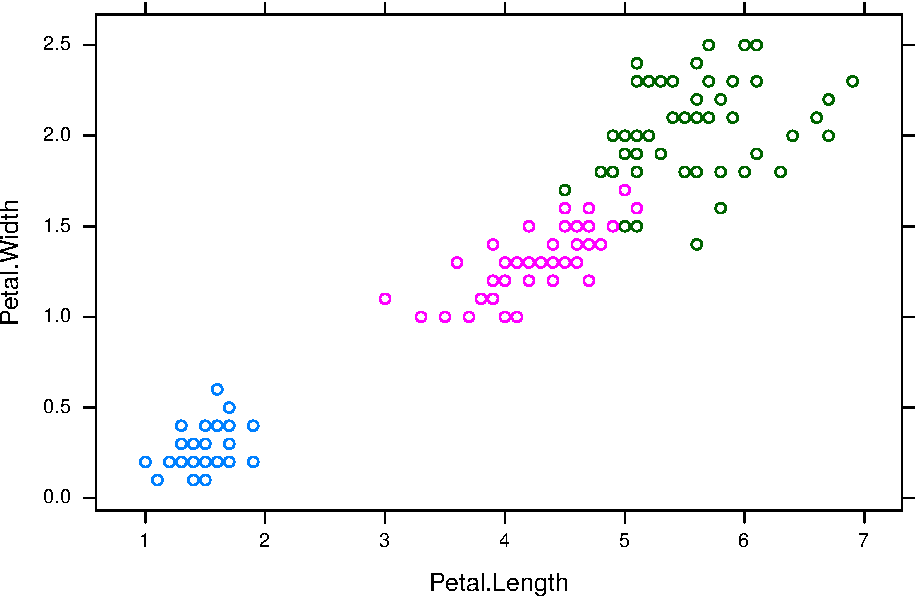
\includegraphics{_main_files/figure-latex/unnamed-chunk-70-1.pdf}
\caption{\label{fig:unnamed-chunk-70}\small Scatterplot of Petal width versus length in the
\texttt{iris} data.}
\end{figure}




\begin{itemize}
\item
  Scatterplot matrices
\item
  splom( \textasciitilde{}
  cbind(GNP.deflator,GNP,Unemployed,Armed.Forces,Population,Year,Employed),
  data = longley)
\item
  splom( \textasciitilde{} cbind(pop15,pop75,dpi), data =
  LifeCycleSavings)
\item
  splom( \textasciitilde{} cbind(Murder, Assault, Rape), data =
  USArrests)
\item
  splom( \textasciitilde{} cbind(CONT, INTG, DMNR), data =
  USJudgeRatings)
\item
  splom( \textasciitilde{} cbind(area,peri,shape,perm), data = rock)
\item
  splom( \textasciitilde{} cbind(Air.Flow, Water.Temp, Acid.Conc.,
  stack.loss), data = stackloss)
\item
  splom( \textasciitilde{}
  cbind(Fertility,Agriculture,Examination,Education,Catholic,Infant.Mortality),
  data = swiss)
\item
  splom(\textasciitilde{} cbind(Fertility,Agriculture,Examination), data
  = swiss) (positive and negative)
\item
  Dot charts
\item
  dotchart(USPersonalExpenditure)
\item
  dotchart(t(USPersonalExpenditure))
\item
  dotchart(WorldPhones) (transpose is no good)
\item
  freeny.x is no good, neither is volcano
\item
  dotchart(UCBAdmissions\{{[}\},,1\{{]}\})
\item
  dotplot(Survived \textasciitilde{} Freq \textbar{} Class, groups =
  Sex, data = B)
\item
  dotplot(Admit \textasciitilde{} Freq \textbar{} Dept, groups = Gender,
  data = C)
\item
  Mosaic plot
\item
  mosaic( \textasciitilde{} Survived + Class + Age + Sex, data =
  Titanic) (or just mosaic(Titanic))
\item
  mosaic( \textasciitilde{} Admit + Dept + Gender, data = UCBAdmissions)
\item
  Spine plots
\item
  spineplot(xtabs(Freq \textasciitilde{} Admit + Gender, data =
  UCBAdmissions))
\item
  rescaled barplot
\item
  Quantile-quantile plots: There are two ways to do this. One way is to
  compare two independent samples (of the same size). qqplot(x,y).
  Another way is to compare the sample quantiles of one variable to the
  theoretical quantiles of another distribution.
\end{itemize}

Given two samples \(x_{1}\), \(x_{2}\), \ldots{}, \(x_{n}\), and
\(y_{1}\), \(y_{2}\), \ldots{}, \(y_{n}\), we may find the order
statistics \(x_{(1)}\leq x_{(2)}\leq\cdots\leq x_{(n)}\) and
\(y_{(1)}\leq y_{(2)}\leq\cdots\leq y_{(n)}\). Next, plot the \(n\)
points \((x_{(1)},y_{(1)})\), \((x_{(2)},y_{(2)})\), \ldots{},
\((x_{(n)},y_{(n)})\).

It is clear that if \(x_{(k)}=y_{(k)}\) for all \(k=1,2,\ldots,n\), then
we will have a straight line. It is also clear that in the real world, a
straight line is NEVER observed, and instead we have a scatterplot that
hopefully had a general linear trend. What do the rules tell us?

\begin{itemize}
\tightlist
\item
  If the \(y\)-intercept of the line is greater (less) than zero, then
  the center of the \(Y\) data is greater (less) than the center of the
  \(X\) data.
\item
  If the slope of the line is greater (less) than one, then the spread
  of the \(Y\) data is greater (less) than the spread of the \(X\) data.
\end{itemize}

\subsection{Lattice Graphics}\label{sub-lattice-graphics}

The following types of plots are useful when there is one variable of
interest and there is a factor in the data set by which the variable is
categorized.

It is sometimes nice to set
\texttt{lattice.options(default.theme\ =\ "col.whitebg")}

\subsubsection{Side by side boxplots}\label{side-by-side-boxplots}

\begin{Shaded}
\begin{Highlighting}[]
\KeywordTok{bwplot}\NormalTok{(~weight |}\StringTok{ }\NormalTok{feed, }\DataTypeTok{data =} \NormalTok{chickwts)}
\end{Highlighting}
\end{Shaded}

\begin{figure}[htbp]
\centering
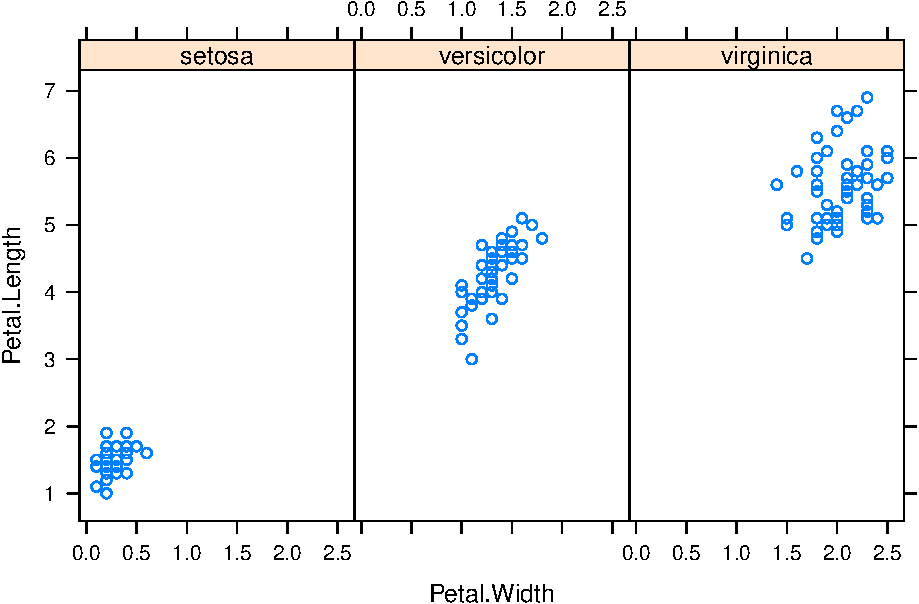
\includegraphics{_main_files/figure-latex/unnamed-chunk-72-1.pdf}
\caption{\label{fig:unnamed-chunk-72}\small Boxplots of \texttt{weight} by \texttt{feed}
type in the \texttt{chickwts} data.}
\end{figure}




\subsubsection{Histograms}\label{histograms}

\begin{Shaded}
\begin{Highlighting}[]
\KeywordTok{histogram}\NormalTok{(~age |}\StringTok{ }\NormalTok{education, }\DataTypeTok{data =} \NormalTok{infert)}
\end{Highlighting}
\end{Shaded}

\begin{figure}[htbp]
\centering
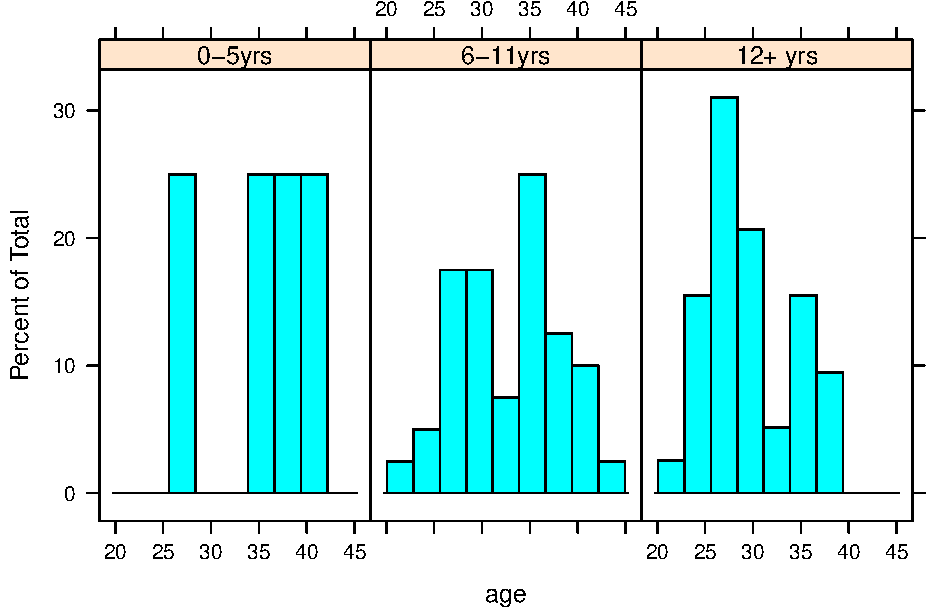
\includegraphics{_main_files/figure-latex/unnamed-chunk-74-1.pdf}
\caption{\label{fig:unnamed-chunk-74}\small Histograms of \texttt{age} by \texttt{education}
level from the \texttt{infert} data.}
\end{figure}




\subsubsection{Scatterplots}\label{scatterplots}

\begin{Shaded}
\begin{Highlighting}[]
\KeywordTok{xyplot}\NormalTok{(Petal.Length ~}\StringTok{ }\NormalTok{Petal.Width |}\StringTok{ }\NormalTok{Species, }\DataTypeTok{data =} \NormalTok{iris)}
\end{Highlighting}
\end{Shaded}

\begin{figure}[htbp]
\centering
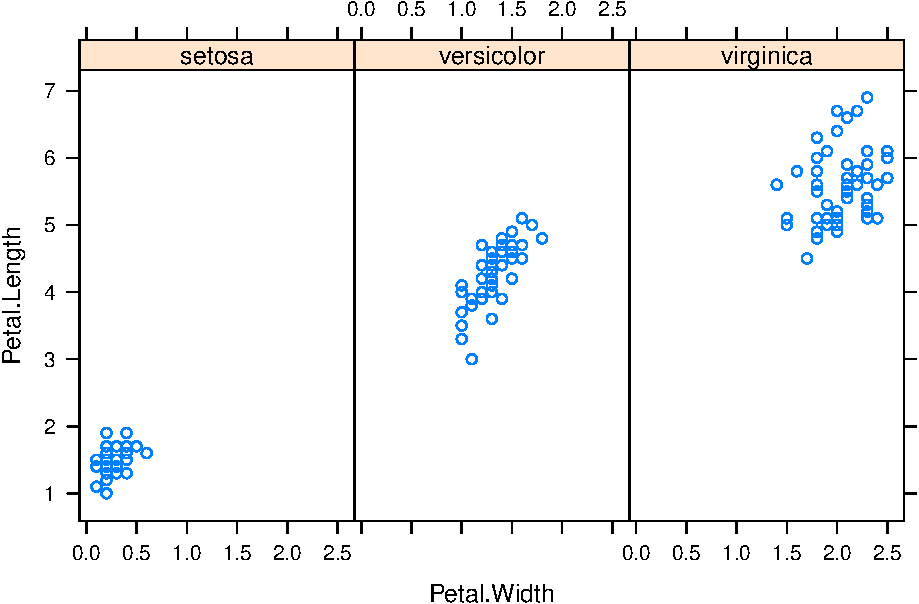
\includegraphics{_main_files/figure-latex/unnamed-chunk-76-1.pdf}
\caption{\label{fig:unnamed-chunk-76}\small An \texttt{xyplot} of \texttt{Petal.Length}
versus \texttt{Petal.Width} by \texttt{Species} in the \texttt{iris}
data.}
\end{figure}





\subsubsection{Coplots}\label{coplots}

\begin{Shaded}
\begin{Highlighting}[]
\KeywordTok{coplot}\NormalTok{(conc ~}\StringTok{ }\NormalTok{uptake |}\StringTok{ }\NormalTok{Type *}\StringTok{ }\NormalTok{Treatment, }\DataTypeTok{data =} \NormalTok{CO2)}
\end{Highlighting}
\end{Shaded}

\begin{figure}[htbp]
\centering
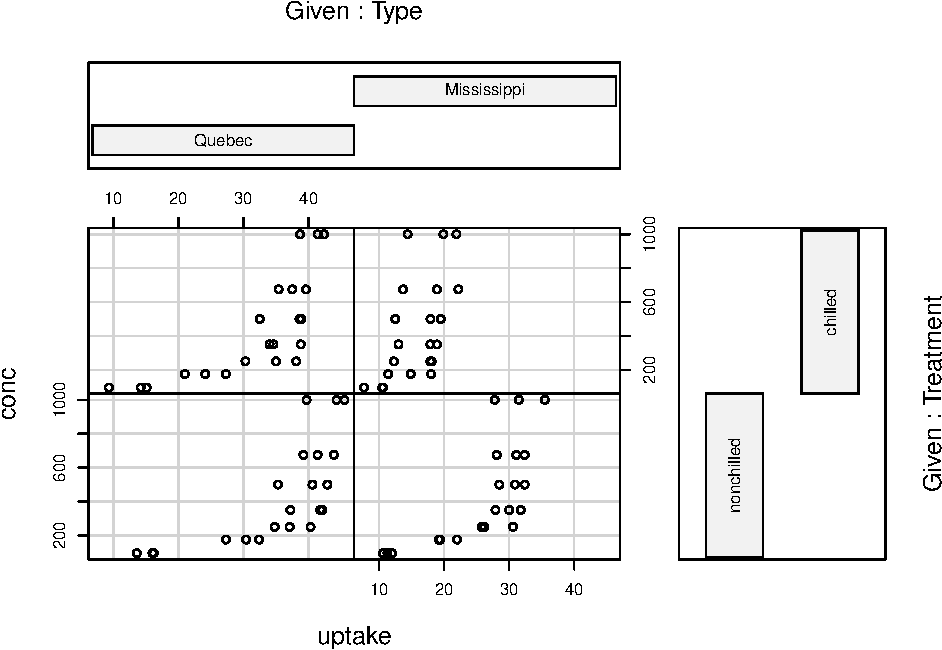
\includegraphics{_main_files/figure-latex/unnamed-chunk-78-1.pdf}
\caption{\label{fig:unnamed-chunk-78}\small A \texttt{coplot} of \texttt{conc} versus
\texttt{uptake} by \texttt{Type} and \texttt{Treatment}.}
\end{figure}

\begin{verbatim}
NULL
\end{verbatim}




\section{Exercises}\label{exercises-1}

Open R and issue the following commands at the command line to get
started. Note that you need to have the \texttt{RcmdrPlugin.IPSUR}
package \autocite{RcmdrPlugin.IPSUR} installed, and for some exercises
you need the \texttt{e1071} package \autocite{e1071}.

\begin{Shaded}
\begin{Highlighting}[]
\KeywordTok{library}\NormalTok{(}\StringTok{"RcmdrPlugin.IPSUR"}\NormalTok{)}
\KeywordTok{data}\NormalTok{(RcmdrTestDrive)}
\KeywordTok{attach}\NormalTok{(RcmdrTestDrive)}
\KeywordTok{names}\NormalTok{(RcmdrTestDrive)}
\end{Highlighting}
\end{Shaded}

To load the data in the R Commander (\texttt{Rcmdr}), click the
\texttt{Data\ Set} button, and select \texttt{RcmdrTestDrive} as the
active data set. To learn more about the data set and where it comes
from, type \texttt{?RcmdrTestDrive} at the command line.

\begin{xca}
Perform a summary of all variables in \texttt{RcmdrTestDrive}. You can
do this with the command \texttt{summary(RcmdrTestDrive)}.

Alternatively, you can do this in the \texttt{Rcmdr} with the sequence
\texttt{Statistics} \(\triangleright\) \texttt{Summaries}
\(\triangleright\) \texttt{Active\ Data\ Set}. Report the values of the
summary statistics for each variable.
\end{xca}

\bigskip

\begin{xca}
Make a table of the \texttt{race} variable. Do this with
\texttt{Statistics} \(\triangleright\) \texttt{Summaries}
\(\triangleright\) \texttt{Frequency\ Distributions\ -\ IPSUR...} 1.
Which ethnicity has the highest frequency? 1. Which ethnicity has the
lowest frequency? 1. Include a bar graph of \texttt{race}. Do this with
\texttt{Graphs} \(\triangleright\) \texttt{IPSUR\ -\ Bar\ Graph...}
\end{xca}

\bigskip

\begin{xca}
Calculate the average \texttt{salary} by the factor \texttt{gender}. Do
this with \texttt{Statistics} \(\triangleright\) \texttt{Summaries}
\(\triangleright\) \texttt{Table\ of\ Statistics...}

\begin{enumerate}
\def\labelenumi{\arabic{enumi}.}
\item
  Which \texttt{gender} has the highest mean \texttt{salary}?
\item
  Report the highest mean \texttt{salary}.
\item
  Compare the spreads for the genders by calculating the standard
  deviation of \texttt{salary} by \texttt{gender}. Which \texttt{gender}
  has the biggest standard deviation?
\item
  Make boxplots of \texttt{salary} by \texttt{gender} with the following
  method:

  \begin{enumerate}
  \def\labelenumii{\roman{enumii})}
  \tightlist
  \item
    On the \texttt{Rcmdr}, click \texttt{Graphs} \(\triangleright\)
    \texttt{IPSUR\ -\ Boxplot...}
  \item
    In the \texttt{Variable} box, select \texttt{salary}.
  \item
    Click the \texttt{Plot\ by\ groups...} box and select
    \texttt{gender}. Click \texttt{OK}.
  \item
    Click \texttt{OK} to graph the boxplot.
  \end{enumerate}
\end{enumerate}

How does the boxplot compare to your answers to (1) and (3)?
\end{xca}

\bigskip

\begin{xca}
For this problem we will study the variable \texttt{reduction}.

\begin{enumerate}
\def\labelenumi{\arabic{enumi}.}
\tightlist
\item
  Find the order statistics and store them in a vector \texttt{x}.
  \emph{Hint:} \texttt{x\ \textless{}-\ sort(reduction)}
\item
  Find \(x_{(137)}\), the 137\(^{\mathrm{th}}\) order statistic.
\item
  Find the IQR.
\item
  Find the Five Number Summary (5NS).
\item
  Use the 5NS to calculate what the width of a boxplot of
  \texttt{reduction} would be.
\item
  Compare your answers (3) and (5). Are they the same? If not, are they
  close?
\item
  Make a boxplot of \texttt{reduction}, and include the boxplot in your
  report. You can do this with the \texttt{boxplot} function, or in
  \texttt{Rcmdr} with \texttt{Graphs} \(\triangleright\)
  \texttt{IPSUR\ -\ Boxplot...}
\item
  Are there any potential/suspected outliers? If so, list their values.
  \emph{Hint:} use your answer to (a).
\item
  Using the rules discussed in the text, classify answers to (8), if
  any, as \emph{potential} or \emph{suspected} outliers.
\end{enumerate}
\end{xca}

\bigskip

\begin{xca}
In this problem we will compare the variables \texttt{before} and
\texttt{after}. Don't forget \texttt{library("e1071")}.

\begin{enumerate}
\def\labelenumi{\arabic{enumi}.}
\tightlist
\item
  Examine the two measures of center for both variables. Judging from
  these measures, which variable has a higher center?
\item
  Which measure of center is more appropriate for \texttt{before}? (You
  may want to look at a boxplot.) Which measure of center is more
  appropriate for \texttt{after}?
\item
  Based on your answer to (2), choose an appropriate measure of spread
  for each variable, calculate it, and report its value. Which variable
  has the biggest spread? (Note that you need to make sure that your
  measures are on the same scale.)
\item
  Calculate and report the skewness and kurtosis for \texttt{before}.
  Based on these values, how would you describe the shape of
  \texttt{before}?
\item
  Calculate and report the skewness and kurtosis for \texttt{after}.
  Based on these values, how would you describe the shape of
  \texttt{after}?
\item
  Plot histograms of \texttt{before} and \texttt{after} and compare them
  to your answers to (4) and (5).
\end{enumerate}
\end{xca}

\bigskip

\begin{xca}
Describe the following data sets just as if you were communicating with
an alien, but one who has had a statistics class. Mention the salient
features (data type, important properties, anything special). Support
your answers with the appropriate visual displays and descriptive
statistics.

\begin{enumerate}
\def\labelenumi{\arabic{enumi}.}
\tightlist
\item
  Conversion rates of Euro currencies stored in \texttt{euro}.
\item
  State abbreviations stored in \texttt{state.abb}.
\item
  Areas of the world's landmasses stored in \texttt{islands}.
\item
  Areas of the 50 United States stored in \texttt{state.area}.
\item
  Region of the 50 United States stored in \texttt{state.region}.
\end{enumerate}
\end{xca}

\chapter{Probability}\label{cha-probability}

In this chapter we define the basic terminology associated with
probability and derive some of its properties. We discuss three
interpretations of probability. We discuss conditional probability and
independent events, along with Bayes' Theorem. We finish the chapter
with an introduction to random variables, which paves the way for the
next two chapters.

In this book we distinguish between two types of experiments:
\emph{deterministic} and \emph{random}. A \emph{deterministic}
experiment is one whose outcome may be predicted with certainty
beforehand, such as combining Hydrogen and Oxygen, or adding two numbers
such as \(2+3\). A \emph{random} experiment is one whose outcome is
determined by chance. We posit that the outcome of a random experiment
may not be predicted with certainty beforehand, even in principle.
Examples of random experiments include tossing a coin, rolling a die,
and throwing a dart on a board, how many red lights you encounter on the
drive home, how many ants traverse a certain patch of sidewalk over a
short period, \emph{etc}.

\emph{What do I want them to know?}

\begin{itemize}
\tightlist
\item
  that there are multiple interpretations of probability, and the
  methods used depend somewhat on the philosophy chosen
\item
  nuts and bolts of basic probability jargon: sample spaces, events,
  probability functions, \emph{etc}.
\item
  how to count
\item
  conditional probability and its relationship with independence
\item
  Bayes' Rule and how it relates to the subjective view of probability
\item
  what we mean by `random variables', and where they come from
\end{itemize}

\begin{figure}[htbp]
\centering
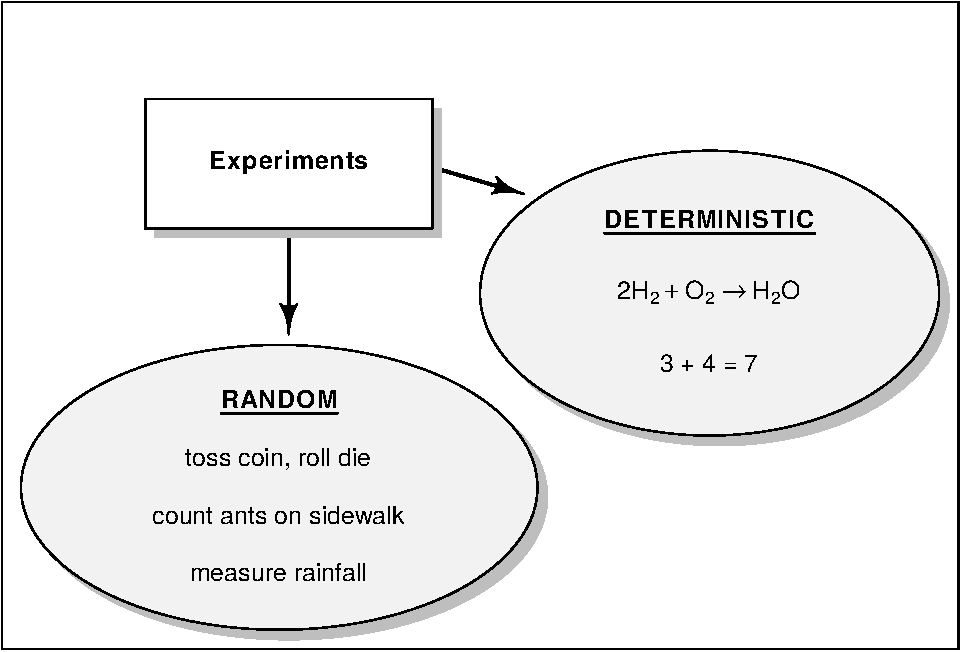
\includegraphics{_main_files/figure-latex/diagram-1.pdf}
\caption{\label{fig:diagram}\small Two types of experiments.}
\end{figure}



\section{Sample Spaces}\label{sec-sample-spaces}

For a random experiment \(E\), the set of all possible outcomes of \(E\)
is called the \emph{sample space} \index{sample space} and is denoted by
the letter \(S\). For a coin-toss experiment, \(S\) would be the results
``Head'' and ``Tail'', which we may represent by \(S = \{H,T \}\).
Formally, the performance of a random experiment is the unpredictable
selection of an outcome in \(S\).

\subsection{How to do it with R}\label{how-to-do-it-with-r-8}

Most of the probability work in this book is done with the \texttt{prob}
package \autocite{prob}. A sample space is (usually) represented by a
\emph{data frame}, that is, a rectangular collection of variables (see
Section \ref{sub-multivariate-data}). Each row of the data frame
corresponds to an outcome of the experiment. The data frame choice is
convenient both for its simplicity and its compatibility with the R
Commander. Data frames alone are, however, not sufficient to describe
some of the more interesting probabilistic applications we will study
later; to handle those we will need to consider a more general
\emph{list} data structure. See Section \ref{sub-howto-ps-objects} for
details.

\bigskip

\BeginKnitrBlock{example}
\protect\hypertarget{ex:unnamed-chunk-88}{}{\label{ex:unnamed-chunk-88}}Consider
the random experiment of dropping a Styrofoam cup onto the floor from a
height of four feet. The cup hits the ground and eventually comes to
rest. It could land upside down, right side up, or it could land on its
side. We represent these possible outcomes of the random experiment by
the following.
\EndKnitrBlock{example}

\begin{Shaded}
\begin{Highlighting}[]
\NormalTok{S <-}\StringTok{ }\KeywordTok{data.frame}\NormalTok{(}\DataTypeTok{lands =} \KeywordTok{c}\NormalTok{(}\StringTok{"down"}\NormalTok{,}\StringTok{"up"}\NormalTok{,}\StringTok{"side"}\NormalTok{))}
\NormalTok{S}
\end{Highlighting}
\end{Shaded}

\begin{verbatim}
  lands
1  down
2    up
3  side
\end{verbatim}

The sample space \texttt{S} contains the column \texttt{lands} which
stores the outcomes \texttt{down}, \texttt{up}, and \texttt{side}.

Some sample spaces are so common that convenience wrappers were written
to set them up with minimal effort. The underlying machinery that does
the work includes the \texttt{expand.grid} function in the \texttt{base}
package \autocite{base}, \texttt{combn} in the \texttt{combinat} package
\autocite{combinat}, and \texttt{permsn} in the \texttt{prob} package
\autocite{prob}\footnote{We can find solutions of the normal equations
  even when \(\mathbf{X}^{\mathrm{T}}\mathbf{X}\) is not of full rank,
  but the topic falls outside the scope of this book. The interested
  reader can consult an advanced text such as Rao \autocite{Rao1999}.}.

Consider the random experiment of tossing a coin. The outcomes are \(H\)
and \(T\). We can set up the sample space quickly with the
\texttt{tosscoin} function:

\begin{Shaded}
\begin{Highlighting}[]
\KeywordTok{tosscoin}\NormalTok{(}\DecValTok{1}\NormalTok{)}
\end{Highlighting}
\end{Shaded}

\begin{verbatim}
  toss1
1     H
2     T
\end{verbatim}

The number \texttt{1} tells \texttt{tosscoin} that we only want to toss
the coin once. We could toss it three times:

\begin{Shaded}
\begin{Highlighting}[]
\KeywordTok{tosscoin}\NormalTok{(}\DecValTok{3}\NormalTok{)}
\end{Highlighting}
\end{Shaded}

\begin{verbatim}
  toss1 toss2 toss3
1     H     H     H
2     T     H     H
3     H     T     H
4     T     T     H
5     H     H     T
6     T     H     T
7     H     T     T
8     T     T     T
\end{verbatim}

Alternatively we could roll a fair die:

\begin{Shaded}
\begin{Highlighting}[]
\KeywordTok{rolldie}\NormalTok{(}\DecValTok{1}\NormalTok{) }
\end{Highlighting}
\end{Shaded}

\begin{verbatim}
  X1
1  1
2  2
3  3
4  4
5  5
6  6
\end{verbatim}

The \texttt{rolldie} function defaults to a 6-sided die, but we can
specify others with the \texttt{nsides} argument. The command
\texttt{rolldie(3,\ nsides\ =\ 4)} would be used to roll a 4-sided die
three times.

Perhaps we would like to draw one card from a standard set of playing
cards (it is a long data frame):

\begin{Shaded}
\begin{Highlighting}[]
\KeywordTok{head}\NormalTok{(}\KeywordTok{cards}\NormalTok{()) }
\end{Highlighting}
\end{Shaded}

\begin{verbatim}
  rank suit
1    2 Club
2    3 Club
3    4 Club
4    5 Club
5    6 Club
6    7 Club
\end{verbatim}

The \texttt{cards} function that we just used has optional arguments
\texttt{jokers} (if you would like Jokers to be in the deck) and
\texttt{makespace} which we will discuss later. There is also a
\texttt{roulette} function which returns the sample space associated
with one spin on a roulette wheel. There are EU and USA versions
available. Interested readers may contribute any other game or sample
spaces that may be of general interest.

\subsection{Sampling from Urns}\label{sub-sampling-from-urns}

This is perhaps the most fundamental type of random experiment. We have
an urn that contains a bunch of distinguishable objects (balls) inside.
We shake up the urn, reach inside, grab a ball, and take a look. That's
all.

But there are all sorts of variations on this theme. Maybe we would like
to grab more than one ball -- say, two balls. What are all of the
possible outcomes of the experiment now? It depends on how we sample. We
could select a ball, take a look, put it back, and sample again. Another
way would be to select a ball, take a look -- but do not put it back --
and sample again (equivalently, just reach in and grab two balls). There
are certainly more possible outcomes of the experiment in the former
case than in the latter. In the first (second) case we say that sampling
is done \emph{with (without) replacement}.

There is more. Suppose we do not actually keep track of which ball came
first. All we observe are the two balls, and we have no idea about the
order in which they were selected. We call this \emph{unordered
sampling} (in contrast to \emph{ordered}) because the order of the
selections does not matter with respect to what we observe. We might as
well have selected the balls and put them in a bag before looking.

Note that this one general class of random experiments contains as a
special case all of the common elementary random experiments. Tossing a
coin twice is equivalent to selecting two balls labeled \(H\) and \(T\)
from an urn, with replacement. The die-roll experiment is equivalent to
selecting a ball from an urn with six elements, labeled 1 through 6.

\subsubsection{How to do it with R}\label{how-to-do-it-with-r-9}

The \texttt{prob} package \autocite{prob} accomplishes sampling from
urns with the \texttt{urnsamples} \index{urnsamples@\texttt{urnsamples}}
function, which has arguments \texttt{x}, \texttt{size},
\texttt{replace}, and \texttt{ordered}. The argument \texttt{x}
represents the urn from which sampling is to be done. The \texttt{size}
argument tells how large the sample will be. The \texttt{ordered} and
\texttt{replace} arguments are logical and specify how sampling will be
performed. We will discuss each in turn.

\bigskip

\BeginKnitrBlock{example}
\protect\hypertarget{ex:sample-urn-two-from-three}{}{\label{ex:sample-urn-two-from-three}}Let
our urn simply contain three balls, labeled 1, 2, and 3, respectively.
We are going to take a sample of size 2 from the urn.
\EndKnitrBlock{example}

\subsubsection{Ordered, With
Replacement}\label{ordered-with-replacement}

If sampling is with replacement, then we can get any outcome 1, 2, or 3
on any draw. Further, by ``ordered'' we mean that we shall keep track of
the order of the draws that we observe. We can accomplish this in R with

\begin{Shaded}
\begin{Highlighting}[]
\KeywordTok{urnsamples}\NormalTok{(}\DecValTok{1}\NormalTok{:}\DecValTok{3}\NormalTok{, }\DataTypeTok{size =} \DecValTok{2}\NormalTok{, }\DataTypeTok{replace =} \OtherTok{TRUE}\NormalTok{, }\DataTypeTok{ordered =} \OtherTok{TRUE}\NormalTok{)}
\end{Highlighting}
\end{Shaded}

\begin{verbatim}
  X1 X2
1  1  1
2  2  1
3  3  1
4  1  2
5  2  2
6  3  2
7  1  3
8  2  3
9  3  3
\end{verbatim}

Notice that rows 2 and 4 are identical, save for the order in which the
numbers are shown. Further, note that every possible pair of the numbers
1 through 3 are listed. This experiment is equivalent to rolling a
3-sided die twice, which we could have accomplished with
\texttt{rolldie(2,\ nsides\ =\ 3)}.

\subsubsection{Ordered, Without
Replacement}\label{ordered-without-replacement}

Here sampling is without replacement, so we may not observe the same
number twice in any row. Order is still important, however, so we expect
to see the outcomes \texttt{1,2} and \texttt{2,1} somewhere in our data
frame.

\begin{Shaded}
\begin{Highlighting}[]
\KeywordTok{urnsamples}\NormalTok{(}\DecValTok{1}\NormalTok{:}\DecValTok{3}\NormalTok{, }\DataTypeTok{size =} \DecValTok{2}\NormalTok{, }\DataTypeTok{replace =} \OtherTok{FALSE}\NormalTok{, }\DataTypeTok{ordered =} \OtherTok{TRUE}\NormalTok{)}
\end{Highlighting}
\end{Shaded}

\begin{verbatim}
  X1 X2
1  1  2
2  2  1
3  1  3
4  3  1
5  2  3
6  3  2
\end{verbatim}

This is just as we expected. Notice that there are less rows in this
answer due to the more restrictive sampling procedure. If the numbers 1,
2, and 3 represented ``Fred'', ``Mary'', and ``Sue'', respectively, then
this experiment would be equivalent to selecting two people of the three
to serve as president and vice-president of a company, respectively, and
the sample space shown above lists all possible ways that this could be
done.

\subsubsection{Unordered, Without
Replacement}\label{unordered-without-replacement}

Again, we may not observe the same outcome twice, but in this case, we
will only retain those outcomes which (when jumbled) would not duplicate
earlier ones.

\begin{Shaded}
\begin{Highlighting}[]
\KeywordTok{urnsamples}\NormalTok{(}\DecValTok{1}\NormalTok{:}\DecValTok{3}\NormalTok{, }\DataTypeTok{size =} \DecValTok{2}\NormalTok{, }\DataTypeTok{replace =} \OtherTok{FALSE}\NormalTok{, }\DataTypeTok{ordered =} \OtherTok{FALSE}\NormalTok{) }
\end{Highlighting}
\end{Shaded}

\begin{verbatim}
  X1 X2
1  1  2
2  1  3
3  2  3
\end{verbatim}

This experiment is equivalent to reaching in the urn, picking a pair,
and looking to see what they are. This is the default setting of
\texttt{urnsamples}, so we would have received the same output by simply
typing \texttt{urnsamples(1:3,\ 2)}.

\subsubsection{Unordered, With
Replacement}\label{unordered-with-replacement}

The last possibility is perhaps the most interesting. We replace the
balls after every draw, but we do not remember the order in which the
draws came.

\begin{Shaded}
\begin{Highlighting}[]
\KeywordTok{urnsamples}\NormalTok{(}\DecValTok{1}\NormalTok{:}\DecValTok{3}\NormalTok{, }\DataTypeTok{size =} \DecValTok{2}\NormalTok{, }\DataTypeTok{replace =} \OtherTok{TRUE}\NormalTok{, }\DataTypeTok{ordered =} \OtherTok{FALSE}\NormalTok{) }
\end{Highlighting}
\end{Shaded}

\begin{verbatim}
  X1 X2
1  1  1
2  1  2
3  1  3
4  2  2
5  2  3
6  3  3
\end{verbatim}

We may interpret this experiment in a number of alternative ways. One
way is to consider this as simply putting two 3-sided dice in a cup,
shaking the cup, and looking inside -- as in a game of \emph{Liar's
Dice}, for instance. Each row of the sample space is a potential pair we
could observe. Another way is to view each outcome as a separate method
to distribute two identical golf balls into three boxes labeled 1, 2,
and 3. Regardless of the interpretation, \texttt{urnsamples} lists every
possible way that the experiment can conclude.

Note that the urn does not need to contain numbers; we could have just
as easily taken our urn to be \texttt{x\ =\ c("Red","Blue","Green")}.
But, there is an \emph{important} point to mention before proceeding.
Astute readers will notice that in our example, the balls in the urn
were \emph{distinguishable} in the sense that each had a unique label to
distinguish it from the others in the urn. A natural question would be,
``What happens if your urn has indistinguishable elements, for example,
what if \texttt{x\ =\ c("Red","Red","Blue")}?'' The answer is that
\texttt{urnsamples} behaves as if each ball in the urn is
distinguishable, regardless of its actual contents. We may thus imagine
that while there are two red balls in the urn, the balls are such that
we can tell them apart (in principle) by looking closely enough at the
imperfections on their surface.

In this way, when the \texttt{x} argument of \texttt{urnsamples} has
repeated elements, the resulting sample space may appear to be
\texttt{ordered\ =\ TRUE} even when, in fact, the call to the function
was \texttt{urnsamples(...,\ ordered\ =\ FALSE)}. Similar remarks apply
for the \texttt{replace} argument.

\section{Events}\label{sec-events}

An \emph{event} \index{event} \(A\) is merely a collection of outcomes,
or in other words, a subset of the sample space\footnote{We are taking
  great leaps over the mathematical details. In particular, we have yet
  to show that \(s^{2}\) has a chi-square distribution and we have not
  even come close to showing that \(b_{i}\) and \(s_{b_{i}}\) are
  independent. But these are entirely outside the scope of the present
  book and the reader may rest assured that the proofs await in later
  classes. See C.R. Rao for more.}. After the performance of a random
experiment \(E\) we say that the event \(A\) \emph{occurred} if the
experiment's outcome belongs to \(A\). We say that a bunch of events
\(A_{1}\), \(A_{2}\), \(A_{3}\), \ldots{} are \emph{mutually exclusive}
\index{mutually exclusive} or \emph{disjoint} if
\(A_{i}\cap A_{j}=\emptyset\) for any distinct pair \(A_{i}\neq A_{j}\).
For instance, in the coin-toss experiment the events
\(A = \{ \mbox{Heads} \}\) and \(B = \{ \mbox{Tails} \}\) would be
mutually exclusive. Now would be a good time to review the algebra of
sets in Appendix \ref{sec-the-algebra-of}.

\subsection{How to do it with R}\label{how-to-do-it-with-r-10}

Given a data frame sample/probability space \texttt{S}, we may extract
rows using the \texttt{{[}{]}} operator:

\begin{Shaded}
\begin{Highlighting}[]
\NormalTok{S <-}\StringTok{ }\KeywordTok{tosscoin}\NormalTok{(}\DecValTok{2}\NormalTok{, }\DataTypeTok{makespace =} \OtherTok{TRUE}\NormalTok{) }
\NormalTok{S[}\DecValTok{1}\NormalTok{:}\DecValTok{3}\NormalTok{, ] }
\end{Highlighting}
\end{Shaded}

\begin{verbatim}
  toss1 toss2 probs
1     H     H  0.25
2     T     H  0.25
3     H     T  0.25
\end{verbatim}

\begin{Shaded}
\begin{Highlighting}[]
\NormalTok{S[}\KeywordTok{c}\NormalTok{(}\DecValTok{2}\NormalTok{,}\DecValTok{4}\NormalTok{), ] }
\end{Highlighting}
\end{Shaded}

\begin{verbatim}
  toss1 toss2 probs
2     T     H  0.25
4     T     T  0.25
\end{verbatim}

and so forth. We may also extract rows that satisfy a logical expression
using the \texttt{subset} function, for instance

\begin{Shaded}
\begin{Highlighting}[]
\NormalTok{S <-}\StringTok{ }\KeywordTok{cards}\NormalTok{() }
\end{Highlighting}
\end{Shaded}

\begin{Shaded}
\begin{Highlighting}[]
\KeywordTok{subset}\NormalTok{(S, suit ==}\StringTok{ "Heart"}\NormalTok{) }
\end{Highlighting}
\end{Shaded}

\begin{verbatim}
   rank  suit
27    2 Heart
28    3 Heart
29    4 Heart
30    5 Heart
31    6 Heart
32    7 Heart
33    8 Heart
34    9 Heart
35   10 Heart
36    J Heart
37    Q Heart
38    K Heart
39    A Heart
\end{verbatim}

\begin{Shaded}
\begin{Highlighting}[]
\KeywordTok{subset}\NormalTok{(S, rank %in%}\StringTok{ }\DecValTok{7}\NormalTok{:}\DecValTok{9}\NormalTok{)}
\end{Highlighting}
\end{Shaded}

\begin{verbatim}
   rank    suit
6     7    Club
7     8    Club
8     9    Club
19    7 Diamond
20    8 Diamond
21    9 Diamond
32    7   Heart
33    8   Heart
34    9   Heart
45    7   Spade
46    8   Spade
47    9   Spade
\end{verbatim}

We could continue indefinitely. Also note that mathematical expressions
are allowed:

\begin{Shaded}
\begin{Highlighting}[]
\KeywordTok{subset}\NormalTok{(}\KeywordTok{rolldie}\NormalTok{(}\DecValTok{3}\NormalTok{), X1+X2+X3 >}\StringTok{ }\DecValTok{16}\NormalTok{) }
\end{Highlighting}
\end{Shaded}

\begin{verbatim}
    X1 X2 X3
180  6  6  5
210  6  5  6
215  5  6  6
216  6  6  6
\end{verbatim}

\subsection{Functions for Finding
Subsets}\label{functions-for-finding-subsets}

It does not take long before the subsets of interest become complicated
to specify. Yet the main idea remains: we have a particular logical
condition to apply to each row. If the row satisfies the condition, then
it should be in the subset. It should not be in the subset otherwise.
The ease with which the condition may be coded depends of course on the
question being asked. Here are a few functions to get started.

\subsubsection{\texorpdfstring{The \texttt{\%in\%}
function}{The \%in\% function}}\label{the-in-function}

The function \texttt{\%in\%} helps to learn whether each value of one
vector lies somewhere inside another vector.

\begin{Shaded}
\begin{Highlighting}[]
\NormalTok{x <-}\StringTok{ }\DecValTok{1}\NormalTok{:}\DecValTok{10} 
\NormalTok{y <-}\StringTok{ }\DecValTok{8}\NormalTok{:}\DecValTok{12} 
\NormalTok{y %in%}\StringTok{ }\NormalTok{x}
\end{Highlighting}
\end{Shaded}

\begin{verbatim}
[1]  TRUE  TRUE  TRUE FALSE FALSE
\end{verbatim}

Notice that the returned value is a vector of length 5 which tests
whether each element of \texttt{y} is in \texttt{x}, in turn.

\subsubsection{\texorpdfstring{The \texttt{isin}
function}{The isin function}}\label{the-isin-function}

It is more common to want to know whether the \emph{whole} vector
\texttt{y} is in \texttt{x}. We can do this with the \texttt{isin}
function.

\begin{Shaded}
\begin{Highlighting}[]
\KeywordTok{isin}\NormalTok{(x,y) }
\end{Highlighting}
\end{Shaded}

\begin{verbatim}
[1] FALSE
\end{verbatim}

Of course, one may ask why we did not try something like
\texttt{all(y\ \%in\%\ x)}, which would give a single result,
\texttt{TRUE}. The reason is that the answers are different in the case
that \texttt{y} has repeated values. Compare:

\begin{Shaded}
\begin{Highlighting}[]
\NormalTok{x <-}\StringTok{ }\DecValTok{1}\NormalTok{:}\DecValTok{10} 
\NormalTok{y <-}\StringTok{ }\KeywordTok{c}\NormalTok{(}\DecValTok{3}\NormalTok{,}\DecValTok{3}\NormalTok{,}\DecValTok{7}\NormalTok{) }
\end{Highlighting}
\end{Shaded}

\begin{Shaded}
\begin{Highlighting}[]
\KeywordTok{all}\NormalTok{(y %in%}\StringTok{ }\NormalTok{x)}
\end{Highlighting}
\end{Shaded}

\begin{verbatim}
[1] TRUE
\end{verbatim}

\begin{Shaded}
\begin{Highlighting}[]
\KeywordTok{isin}\NormalTok{(x,y) }
\end{Highlighting}
\end{Shaded}

\begin{verbatim}
[1] FALSE
\end{verbatim}

The reason for the above is of course that \texttt{x} contains the value
3, but \texttt{x} does not have \emph{two} 3's. The difference is
important when rolling multiple dice, playing cards, \emph{etc}. Note
that there is an optional argument \texttt{ordered} which tests whether
the elements of \texttt{y} appear in \texttt{x} in the order in which
they are appear in \texttt{y}. The consequences are

\begin{Shaded}
\begin{Highlighting}[]
\KeywordTok{isin}\NormalTok{(x, }\KeywordTok{c}\NormalTok{(}\DecValTok{3}\NormalTok{,}\DecValTok{4}\NormalTok{,}\DecValTok{5}\NormalTok{), }\DataTypeTok{ordered =} \OtherTok{TRUE}\NormalTok{) }
\end{Highlighting}
\end{Shaded}

\begin{verbatim}
[1] TRUE
\end{verbatim}

\begin{Shaded}
\begin{Highlighting}[]
\KeywordTok{isin}\NormalTok{(x, }\KeywordTok{c}\NormalTok{(}\DecValTok{3}\NormalTok{,}\DecValTok{5}\NormalTok{,}\DecValTok{4}\NormalTok{), }\DataTypeTok{ordered =} \OtherTok{TRUE}\NormalTok{) }
\end{Highlighting}
\end{Shaded}

\begin{verbatim}
[1] FALSE
\end{verbatim}

The connection to probability is that have a data frame sample space and
we would like to find a subset of that space. A \texttt{data.frame}
method was written for \texttt{isin} that simply applies the function to
each row of the data frame. We can see the method in action with the
following:

\begin{Shaded}
\begin{Highlighting}[]
\NormalTok{S <-}\StringTok{ }\KeywordTok{rolldie}\NormalTok{(}\DecValTok{4}\NormalTok{) }
\KeywordTok{subset}\NormalTok{(S, }\KeywordTok{isin}\NormalTok{(S, }\KeywordTok{c}\NormalTok{(}\DecValTok{2}\NormalTok{,}\DecValTok{2}\NormalTok{,}\DecValTok{6}\NormalTok{), }\DataTypeTok{ordered =} \OtherTok{TRUE}\NormalTok{)) }
\end{Highlighting}
\end{Shaded}

\begin{verbatim}
     X1 X2 X3 X4
188   2  2  6  1
404   2  2  6  2
620   2  2  6  3
836   2  2  6  4
1052  2  2  6  5
1088  2  2  1  6
1118  2  1  2  6
1123  1  2  2  6
1124  2  2  2  6
1125  3  2  2  6
1126  4  2  2  6
1127  5  2  2  6
1128  6  2  2  6
1130  2  3  2  6
1136  2  4  2  6
1142  2  5  2  6
1148  2  6  2  6
1160  2  2  3  6
1196  2  2  4  6
1232  2  2  5  6
1268  2  2  6  6
\end{verbatim}

There are a few other functions written to find useful subsets, namely,
\texttt{countrep} and \texttt{isrep}. Essentially these were written to
test for (or count) a specific number of designated values in outcomes.
See the documentation for details.

\subsection{Set Union, Intersection, and
Difference}\label{set-union-intersection-and-difference}

Given subsets \(A\) and \(B\), it is often useful to manipulate them in
an algebraic fashion. To this end, we have three set operations at our
disposal: union, intersection, and difference. Below is a table that
summarizes the pertinent information about these operations.

\begin{longtable}[]{@{}llll@{}}
\caption{Basic set operations. The first column lists the name, the
second shows the typical notation, the third describes set membership,
and the fourth shows how to accomplish it with R.}\tabularnewline
\toprule
Name & Denoted & Defined by elements & Code\tabularnewline
\midrule
\endfirsthead
\toprule
Name & Denoted & Defined by elements & Code\tabularnewline
\midrule
\endhead
Union & \(A\cup B\) & in \(A\) or \(B\) or both &
\texttt{union(A,B)}\tabularnewline
Intersection & \(A\cap B\) & in both \(A\) and \(B\) &
\texttt{intersect(A,B)}\tabularnewline
Difference & \(A\backslash B\) & in \(A\) but not in \(B\) &
\texttt{setdiff(A,B)}\tabularnewline
\bottomrule
\end{longtable}

Some examples follow.

\begin{Shaded}
\begin{Highlighting}[]
\NormalTok{S <-}\StringTok{ }\KeywordTok{cards}\NormalTok{() }
\NormalTok{A <-}\StringTok{ }\KeywordTok{subset}\NormalTok{(S, suit ==}\StringTok{ "Heart"}\NormalTok{) }
\NormalTok{B <-}\StringTok{ }\KeywordTok{subset}\NormalTok{(S, rank %in%}\StringTok{ }\DecValTok{7}\NormalTok{:}\DecValTok{9}\NormalTok{)}
\end{Highlighting}
\end{Shaded}

We can now do some set algebra:

\begin{Shaded}
\begin{Highlighting}[]
\KeywordTok{union}\NormalTok{(A,B)}
\end{Highlighting}
\end{Shaded}

\begin{verbatim}
   rank    suit
6     7    Club
7     8    Club
8     9    Club
19    7 Diamond
20    8 Diamond
21    9 Diamond
27    2   Heart
28    3   Heart
29    4   Heart
30    5   Heart
31    6   Heart
32    7   Heart
33    8   Heart
34    9   Heart
35   10   Heart
36    J   Heart
37    Q   Heart
38    K   Heart
39    A   Heart
45    7   Spade
46    8   Spade
47    9   Spade
\end{verbatim}

\begin{Shaded}
\begin{Highlighting}[]
\KeywordTok{intersect}\NormalTok{(A,B)}
\end{Highlighting}
\end{Shaded}

\begin{verbatim}
   rank  suit
32    7 Heart
33    8 Heart
34    9 Heart
\end{verbatim}

\begin{Shaded}
\begin{Highlighting}[]
\KeywordTok{setdiff}\NormalTok{(A,B)}
\end{Highlighting}
\end{Shaded}

\begin{verbatim}
   rank  suit
27    2 Heart
28    3 Heart
29    4 Heart
30    5 Heart
31    6 Heart
35   10 Heart
36    J Heart
37    Q Heart
38    K Heart
39    A Heart
\end{verbatim}

\begin{Shaded}
\begin{Highlighting}[]
\KeywordTok{setdiff}\NormalTok{(B,A) }
\end{Highlighting}
\end{Shaded}

\begin{verbatim}
   rank    suit
6     7    Club
7     8    Club
8     9    Club
19    7 Diamond
20    8 Diamond
21    9 Diamond
45    7   Spade
46    8   Spade
47    9   Spade
\end{verbatim}

Notice that \texttt{setdiff} is not symmetric. Further, note that we can
calculate the \emph{complement} of a set \(A\), denoted \(A^{c}\) and
defined to be the elements of \(S\) that are not in \(A\) simply with
\texttt{setdiff(S,A)}. There have been methods written for
\texttt{intersect}, \texttt{setdiff}, \texttt{subset}, and
\texttt{union} in the case that the input objects are of class
\texttt{ps}. See Section \ref{sub-howto-ps-objects}.

\bigskip

\begin{note}
When the \texttt{prob} package {[}@prob{]} loads you will notice a
message:
\texttt{The\ following\ object(s)\ are\ masked\ from\ package:base:\ intersect,\ setdiff}.
The reason for this message is that there already exist methods for the
functions \texttt{intersect}, \texttt{setdiff}, \texttt{subset}, and
\texttt{union} in the \texttt{base} package which ships with R. However,
these methods were designed for when the arguments are vectors of the
same mode. Since we are manipulating sample spaces which are data frames
and lists, it was necessary to write methods to handle those cases as
well. When the \texttt{prob} package is loaded, R recognizes that there
are multiple versions of the same function in the search path and acts
to shield the new definitions from the existing ones. But there is no
cause for alarm, thankfully, because the \texttt{prob} functions have
been carefully defined to match the usual \texttt{base} package
definition in the case that the arguments are vectors.
\end{note}

\section{Model Assignment}\label{sec-interpreting-probabilities}

Let us take a look at the coin-toss experiment more closely. What do we
mean when we say ``the probability of Heads'' or write
\(\mathbb{P}(\mbox{Heads})\)? Given a coin and an itchy thumb, how do we
go about finding what \(\mathbb{P}(\mbox{Heads})\) should be?

\subsection{The Measure Theory
Approach}\label{the-measure-theory-approach}

This approach states that the way to handle \(\mathbb{P}(\mbox{Heads})\)
is to define a mathematical function, called a \emph{probability
measure}, on the sample space. Probability measures satisfy certain
axioms (to be introduced later) and have special mathematical
properties, so not just any mathematical function will do. But in any
given physical circumstance there are typically all sorts of probability
measures from which to choose, and it is left to the experimenter to
make a reasonable choice -- one usually based on considerations of
objectivity. For the tossing coin example, a valid probability measure
assigns probability \(p\) to the event \(\{ \mbox{Heads} \}\), where
\(p\) is some number \(0\leq p\leq1\). An experimenter that wishes to
incorporate the symmetry of the coin would choose \(p=1/2\) to balance
the likelihood of \(\{\mbox{Heads} \}\) and \(\{ \mbox{Tails} \}\).

Once the probability measure is chosen (or determined), there is not
much left to do. All assignments of probability are made by the
probability function, and the experimenter needs only to plug the event
\(\{ \mbox{Heads} \}\) into to the probability function to find
\(\mathbb{P}(\mbox{Heads})\). In this way, the probability of an event
is simply a calculated value, nothing more, nothing less. Of course this
is not the whole story; there are many theorems and consequences
associated with this approach that will keep us occupied for the
remainder of this book. The approach is called \emph{measure theory}
because the measure (probability) of a set (event) is associated with
how big it is (how likely it is to occur).

The measure theory approach is well suited for situations where there is
symmetry to the experiment, such as flipping a balanced coin or spinning
an arrow around a circle with well-defined pie slices. It is also handy
because of its mathematical simplicity, elegance, and flexibility. There
are literally volumes of information that one can prove about
probability measures, and the cold rules of mathematics allow us to
analyze intricate probabilistic problems with vigor.

The large degree of flexibility is also a disadvantage, however. When
symmetry fails it is not always obvious what an ``objective'' choice of
probability measure should be; for instance, what probability should we
assign to \(\{ \mbox{Heads} \}\) if we spin the coin rather than flip
it? (It is not \(1/2\).) Furthermore, the mathematical rules are
restrictive when we wish to incorporate subjective knowledge into the
model, knowledge which changes over time and depends on the
experimenter, such as personal knowledge about the properties of the
specific coin being flipped, or of the person doing the flipping.

The mathematician who revolutionized this way to do probability theory
was Andrey Kolmogorov, who published a landmark monograph in 1933. See
\url{http://www-history.mcs.st-andrews.ac.uk/Mathematicians/Kolmogorov.html}
for more information.

\subsection{Relative Frequency
Approach}\label{relative-frequency-approach}

This approach states that the way to determine
\(\mathbb{P}(\mbox{Heads})\) is to flip the coin repeatedly, in exactly
the same way each time. Keep a tally of the number of flips and the
number of Heads observed. Then a good approximation to
\(\mathbb{P}(\mbox{Heads})\) will be

\begin{equation} 
\mathbb{P}(\mbox{Heads})\approx\frac{\mbox{number of observed Heads}}{\mbox{total number of flips}}.
\end{equation}

The mathematical underpinning of this approach is the celebrated
\emph{Law of Large Numbers} which may be loosely described as follows.
Let \(E\) be a random experiment in which the event \(A\) either does or
does not occur. Perform the experiment repeatedly, in an identical
manner, in such a way that the successive experiments do not influence
each other. After each experiment, keep a running tally of whether or
not the event \(A\) occurred. Let \(S_{n}\) count the number of times
that \(A\) occurred in the \(n\) experiments. Then the law of large
numbers says that

\begin{equation}
\frac{S_{n}}{n}\to\mathbb{P}(A)\mbox{ as }n\to\infty.
\end{equation}

As the reasoning goes, to learn about the probability of an event \(A\)
we need only repeat the random experiment to get a reasonable estimate
of the probability's value, and if we are not satisfied with our
estimate then we may simply repeat the experiment more times all the
while confident that with more and more experiments our estimate will
stabilize to the true value.

The frequentist approach is good because it is relatively light on
assumptions and does not worry about symmetry or claims of objectivity
like the measure-theoretic approach does. It is perfect for the spinning
coin experiment. One drawback to the method is that one can never know
the exact value of a probability, only a long-run approximation. It also
does not work well with experiments that can not be repeated
indefinitely, say, the probability that it will rain today, the chances
that you get will get an A in your Statistics class, or the probability
that the world is destroyed by nuclear war.

This approach was espoused by Richard von Mises in the early twentieth
century, and some of his main ideas were incorporated into the measure
theory approach. See
\url{http://www-history.mcs.st-andrews.ac.uk/Biographies/Mises.html} for
more.

\subsection{The Subjective Approach}\label{the-subjective-approach}

The subjective approach interprets probability as the experimenter's
\emph{degree of belief} that the event will occur. The estimate of the
probability of an event is based on the totality of the individual's
knowledge at the time. As new information becomes available, the
estimate is modified accordingly to best reflect his/her current
knowledge. The method by which the probabilities are updated is commonly
done with Bayes' Rule, discussed in Section \ref{sec-bayes-rule}.

So for the coin toss example, a person may have
\(\mathbb{P}(\mbox{Heads})=1/2\) in the absence of additional
information. But perhaps the observer knows additional information about
the coin or the thrower that would shift the probability in a certain
direction. For instance, parlor magicians may be trained to be quite
skilled at tossing coins, and some are so skilled that they may toss a
fair coin and get nothing but Heads, indefinitely. I have \emph{seen}
this. It was similarly claimed in \emph{Bringing Down the House}
\autocite{Mezrich2003} that MIT students were accomplished enough with
cards to be able to cut a deck to the same location, every single time.
In such cases, one clearly should use the additional information to
assign \(\mathbb{P}(\mbox{Heads})\) away from the symmetry value of
\(1/2\).

This approach works well in situations that cannot be repeated
indefinitely, for example, to assign your probability that you will get
an A in this class, the chances of a devastating nuclear war, or the
likelihood that a cure for the common cold will be discovered.

The roots of subjective probability reach back a long time. See
\url{http://en.wikipedia.org/wiki/Subjective_probability} for a short
discussion and links to references about the subjective approach.

\subsection{Equally Likely Model (ELM)}\label{equally-likely-model-elm}

We have seen several approaches to the assignment of a probability model
to a given random experiment and they are very different in their
underlying interpretation. But they all cross paths when it comes to the
equally likely model which assigns equal probability to all elementary
outcomes of the experiment.

The ELM appears in the measure theory approach when the experiment
boasts symmetry of some kind. If symmetry guarantees that all outcomes
have equal ``size'', and if outcomes with equal ``size'' should get the
same probability, then the ELM is a logical objective choice for the
experimenter. Consider the balanced 6-sided die, the fair coin, or the
dart board with equal-sized wedges.

The ELM appears in the subjective approach when the experimenter resorts
to indifference or ignorance with respect to his/her knowledge of the
outcome of the experiment. If the experimenter has no prior knowledge to
suggest that (s)he prefer Heads over Tails, then it is reasonable for
the him/her to assign equal subjective probability to both possible
outcomes.

The ELM appears in the relative frequency approach as a fascinating fact
of Nature: when we flip balanced coins over and over again, we observe
that the proportion of times that the coin comes up Heads tends to
\(1/2\). Of course if we assume that the measure theory applies then we
can prove that the sample proportion must tend to 1/2 as expected, but
that is putting the cart before the horse, in a manner of speaking.

The ELM is only available when there are finitely many elements in the
sample space.

\subsubsection{How to do it with R}\label{how-to-do-it-with-r-11}

In the \texttt{prob} package \autocite{prob}, a probability space is an
object of outcomes \texttt{S} and a vector of probabilities (called
\texttt{probs}) with entries that correspond to each outcome in
\texttt{S}. When \texttt{S} is a data frame, we may simply add a column
called \texttt{probs} to \texttt{S} and we will be finished; the
probability space will simply be a data frame which we may call
\texttt{S}. In the case that S is a list, we may combine the
\texttt{outcomes} and \texttt{probs} into a larger list, \texttt{space};
it will have two components: \texttt{outcomes} and \texttt{probs}. The
only requirements we need are for the entries of \texttt{probs} to be
nonnegative and \texttt{sum(probs)} to be one.

To accomplish this in R, we may use the \texttt{probspace} function. The
general syntax is \texttt{probspace(x,\ probs)}, where \texttt{x} is a
sample space of outcomes and \texttt{probs} is a vector (of the same
length as the number of outcomes in \texttt{x}). The specific choice of
\texttt{probs} depends on the context of the problem, and some examples
follow to demonstrate some of the more common choices.

\bigskip

\BeginKnitrBlock{example}
\protect\hypertarget{ex:unnamed-chunk-116}{}{\label{ex:unnamed-chunk-116}}The
Equally Likely Model asserts that every outcome of the sample space has
the same probability, thus, if a sample space has \(n\) outcomes, then
\texttt{probs} would be a vector of length \(n\) with identical entries
\(1/n\). The quickest way to generate \texttt{probs} is with the
\texttt{rep} function. We will start with the experiment of rolling a
die, so that \(n=6\). We will construct the sample space, generate the
\texttt{probs} vector, and put them together with \texttt{probspace}.
\EndKnitrBlock{example}

\begin{Shaded}
\begin{Highlighting}[]
\NormalTok{outcomes <-}\StringTok{ }\KeywordTok{rolldie}\NormalTok{(}\DecValTok{1}\NormalTok{) }
\NormalTok{p <-}\StringTok{ }\KeywordTok{rep}\NormalTok{(}\DecValTok{1}\NormalTok{/}\DecValTok{6}\NormalTok{, }\DataTypeTok{times =} \DecValTok{6}\NormalTok{) }
\KeywordTok{probspace}\NormalTok{(outcomes, }\DataTypeTok{probs =} \NormalTok{p) }
\end{Highlighting}
\end{Shaded}

\begin{verbatim}
  X1     probs
1  1 0.1666667
2  2 0.1666667
3  3 0.1666667
4  4 0.1666667
5  5 0.1666667
6  6 0.1666667
\end{verbatim}

The \texttt{probspace} function is designed to save us some time in the
most common situations. For example, due to the especial simplicity of
the sample space in this case, we could have achieved the same result
with only (note the name change for the first column)

\begin{Shaded}
\begin{Highlighting}[]
\KeywordTok{probspace}\NormalTok{(}\DecValTok{1}\NormalTok{:}\DecValTok{6}\NormalTok{, }\DataTypeTok{probs =} \NormalTok{p) }
\end{Highlighting}
\end{Shaded}

\begin{verbatim}
  x     probs
1 1 0.1666667
2 2 0.1666667
3 3 0.1666667
4 4 0.1666667
5 5 0.1666667
6 6 0.1666667
\end{verbatim}

Further, since the equally likely model plays such a fundamental role in
the study of probability the \texttt{probspace} function will assume
that the equally model is desired if no \texttt{probs} are specified.
Thus, we get the same answer with only

\begin{Shaded}
\begin{Highlighting}[]
\KeywordTok{probspace}\NormalTok{(}\DecValTok{1}\NormalTok{:}\DecValTok{6}\NormalTok{) }
\end{Highlighting}
\end{Shaded}

\begin{verbatim}
  x     probs
1 1 0.1666667
2 2 0.1666667
3 3 0.1666667
4 4 0.1666667
5 5 0.1666667
6 6 0.1666667
\end{verbatim}

And finally, since rolling dice is such a common experiment in
probability classes, the \texttt{rolldie} function has an additional
logical argument \texttt{makespace} that will add a column of equally
likely \texttt{probs} to the generated sample space:

\begin{Shaded}
\begin{Highlighting}[]
\KeywordTok{rolldie}\NormalTok{(}\DecValTok{1}\NormalTok{, }\DataTypeTok{makespace =} \OtherTok{TRUE}\NormalTok{)}
\end{Highlighting}
\end{Shaded}

\begin{verbatim}
  X1     probs
1  1 0.1666667
2  2 0.1666667
3  3 0.1666667
4  4 0.1666667
5  5 0.1666667
6  6 0.1666667
\end{verbatim}

or just \texttt{rolldie(1,\ TRUE)}. Many of the other sample space
functions (\texttt{tosscoin}, \texttt{cards}, \texttt{roulette},
\emph{etc}.) have similar \texttt{makespace} arguments. Check the
documentation for details.

One sample space function that does NOT have a \texttt{makespace} option
is the \texttt{urnsamples} function. This was intentional. The reason is
that under the varied sampling assumptions the outcomes in the
respective sample spaces are NOT, in general, equally likely. It is
important for the user to carefully consider the experiment to decide
whether or not the outcomes are equally likely and then use
\texttt{probspace} to assign the model.

\bigskip

\BeginKnitrBlock{example}[An unbalanced coin]
\protect\hypertarget{ex:unbalanced-coin}{}{\label{ex:unbalanced-coin}
\iffalse (An unbalanced coin) \fi }While the \texttt{makespace} argument
to \texttt{tosscoin} is useful to represent the tossing of a \emph{fair}
coin, it is not always appropriate. For example, suppose our coin is not
perfectly balanced, for instance, maybe the \(H\) side is somewhat
heavier such that the chances of a \(H\) appearing in a single toss is
0.70 instead of 0.5. We may set up the probability space with
\EndKnitrBlock{example}

\begin{Shaded}
\begin{Highlighting}[]
\KeywordTok{probspace}\NormalTok{(}\KeywordTok{tosscoin}\NormalTok{(}\DecValTok{1}\NormalTok{), }\DataTypeTok{probs =} \KeywordTok{c}\NormalTok{(}\FloatTok{0.70}\NormalTok{, }\FloatTok{0.30}\NormalTok{)) }
\end{Highlighting}
\end{Shaded}

\begin{verbatim}
  toss1 probs
1     H   0.7
2     T   0.3
\end{verbatim}

The same procedure can be used to represent an unbalanced die, roulette
wheel, \emph{etc}.

\subsection{Words of Warning}\label{words-of-warning}

It should be mentioned that while the splendour of R is uncontested, it,
like everything else, has limits both with respect to the
sample/probability spaces it can manage and with respect to the finite
accuracy of the representation of most numbers (see the R FAQ 7.31).
When playing around with probability, one may be tempted to set up a
probability space for tossing 100 coins or rolling 50 dice in an attempt
to answer some scintillating question. (Bear in mind: rolling a die just
9 times has a sample space with over \emph{10 million} outcomes.)

Alas, even if there were enough RAM to barely hold the sample space (and
there were enough time to wait for it to be generated), the
infinitesimal probabilities that are associated with \emph{so many}
outcomes make it difficult for the underlying machinery to handle
reliably. In some cases, special algorithms need to be called just to
give something that holds asymptotically. User beware.

\section{Properties of Probability}\label{sec-properties-of-probability}

\subsection{Probability Functions}\label{sub-probability-functions}

A \emph{probability function} is a rule that associates with each event
\(A\) of the sample space a single number \(\mathbb{P}(A)=p\), called
the \emph{probability of} \(A\). Any probability function \(\mathbb{P}\)
satisfies the following three Kolmogorov Axioms:

\bigskip

\begin{axiom}
\(\mathbb{P}(A)\geq0\) for any event \(A\subset S\).
\end{axiom}

\bigskip

\begin{axiom}
\(\mathbb{P}(S)=1\).
\end{axiom}

\bigskip

\begin{axiom}
If the events \(A_{1}\), \(A_{2}\), \(A_{3}\)\ldots{} are disjoint then

\begin{equation}
\mathbb{P}\left(\bigcup_{i=1}^{n}A_{i}\right)=\sum_{i=1}^{n}\mathbb{P}(A_{i})\mbox{ for every }n,
\end{equation}

and furthermore,

\begin{equation}
\mathbb{P}\left(\bigcup_{i=1}^{\infty}A_{i}\right)=\sum_{i=1}^{\infty}\mathbb{P}(A_{i}).
\end{equation}
\end{axiom}

The intuition behind the axioms goes like this: first, the probability
of an event should never be negative. Second, since the sample space
contains all possible outcomes, its probability should be one, or 100\%.
The last axiom may look intimidating but it simply means that in a
sequence of disjoint events (in other words, sets that do not overlap),
the total probability (measure) should equal the sum of its parts. For
example, the chance of rolling a 1 or a 2 on a die should be the chance
of rolling a 1 plus the chance of rolling a 2.

\subsection{Properties}\label{properties}

For any events \(A\) and \(B\),

\begin{enumerate}
\def\labelenumi{\arabic{enumi}.}
\tightlist
\item
  \textless{}\textgreater{} \(\mathbb{P}(A^{c})=1-\mathbb{P}(A)\).
  \textbf{Proof:} Since \(A\cup A^{c}=S\) and \(A\cap A^{c}=\emptyset\),
  we have \[
     1=\mathbb{P}(S)=\mathbb{P}(A\cup A^{c})=\mathbb{P}(A)+\mathbb{P}(A^{c}).
     \]
\item
  \(\mathbb{P}(\emptyset)=0\). \textbf{Proof:} Note that
  \(\emptyset=S^{c}\), and use Property 1.
\item
  If \(A\subset B\) , then \(\mathbb{P}(A)\leq\mathbb{P}(B)\).
  \textbf{Proof:} Write \(B=A\cup\left(B\cap A^{c}\right)\), and notice
  that \(A\cap\left(B\cap A^{c}\right)=\emptyset\); thus \[
     \mathbb{P}(B)=\mathbb{P}(A\cup\left(B\cap A^{c}\right))=\mathbb{P}(A)+\mathbb{P}\left(B\cap A^{c}\right)\geq\mathbb{P}(A),
     \] since \(\mathbb{P}\left(B\cap A^{c}\right)\ge0\).
\item
  \(0\leq\mathbb{P}(A)\leq1\). \textbf{Proof:} The left inequality is
  immediate from Axiom \ref{ax-prob-nonnegative}, and the second
  inequality follows from Property 3 since \(A\subset S\).
\item
  \textbf{The General Addition Rule.}

  \begin{equation}
     \label{eq-general-addition-rule-1}
     \mathbb{P}(A\cup B)=\mathbb{P}(A)+\mathbb{P}(B)-\mathbb{P}(A\cap B).
     \end{equation}

  More generally, for events \(A_{1}\), \(A_{2}\), \(A_{3}\),\ldots{},
  \(A_{n}\),

  \begin{equation}
     \mathbb{P}\left(\bigcup_{i=1}^{n}A_{i}\right)=\sum_{i=1}^{n}\mathbb{P}(A_{i})-\sum_{i=1}^{n-1}\sum_{j=i+1}^{n}\mathbb{P}(A_{i}\cap A_{j})+\cdots+(-1)^{n-1}\mathbb{P}\left(\bigcap_{i=1}^{n}A_{i}\right)
     \end{equation}
\item
  \textbf{The Theorem of Total Probability.} Let \(B_{1}\), \(B_{2}\),
  \ldots{}, \(B_{n}\) be mutually exclusive and exhaustive. Then

  \begin{equation}
     \label{eq-theorem-total-probability}
     \mathbb{P}(A)=\mathbb{P}(A\cap B_{1})+\mathbb{P}(A\cap B_{2})+\cdots+\mathbb{P}(A\cap B_{n}).
     \end{equation}
\end{enumerate}

\subsection{Assigning Probabilities}\label{assigning-probabilities}

A model of particular interest is the \emph{equally likely model}. The
idea is to divide the sample space \(S\) into a finite collection of
elementary events \(\{ a_{1},\ a_{2}, \ldots, a_{N} \}\) that are
equally likely in the sense that each \(a_{i}\) has equal chances of
occurring. The probability function associated with this model must
satisfy \(\mathbb{P}(S)=1\), by Axiom 2. On the other hand, it must also
satisfy \[ \mathbb{P}(S)=\mathbb{P}( \{ a_{1},\
a_{2},\ldots,a_{N} \} )=\mathbb{P}(a_{1}\cup a_{2}\cup\cdots\cup
a_{N})=\sum_{i=1}^{N}\mathbb{P}(a_{i}), \] by Axiom 3. Since
\(\mathbb{P}(a_{i})\) is the same for all \(i\), each one necessarily
equals \(1/N\).

For an event \(A\subset S\), we write \(A\) as a collection of
elementary outcomes: if
\(A = \{ a_{i_{1}}, a_{i_{2}}, \ldots, a_{i_{k}} \}\) then \(A\) has
\(k\) elements and

\begin{align*}
\mathbb{P}(A) & =\mathbb{P}(a_{i_{1}})+\mathbb{P}(a_{i_{2}})+\cdots+\mathbb{P}(a_{i_{k}}),\\
 & =\frac{1}{N}+\frac{1}{N}+\cdots+\frac{1}{N},\\
 & =\frac{k}{N}=\frac{\#(A)}{\#(S)}.
\end{align*}

In other words, under the equally likely model, the probability of an
event \(A\) is determined by the number of elementary events that \(A\)
contains.

\bigskip

\BeginKnitrBlock{example}
\protect\hypertarget{ex:unnamed-chunk-122}{}{\label{ex:unnamed-chunk-122}}Consider
the random experiment \(E\) of tossing a coin. Then the sample space is
\(S=\{H,T\}\), and under the equally likely model, these two outcomes
have \(\mathbb{P}(H)=\mathbb{P}(T)=1/2\). This model is taken when it is
reasonable to assume that the coin is fair.
\EndKnitrBlock{example}

\bigskip

\BeginKnitrBlock{example}
\protect\hypertarget{ex:unnamed-chunk-123}{}{\label{ex:unnamed-chunk-123}}Suppose
the experiment \(E\) consists of tossing a fair coin twice. The sample
space may be represented by \(S=\{HH,\, HT,\, TH,\, TT\}\). Given that
the coin is fair and that the coin is tossed in an independent and
identical manner, it is reasonable to apply the equally likely model.
\EndKnitrBlock{example}

What is \(\mathbb{P}(\mbox{at least 1 Head})\)? Looking at the sample
space we see the elements \(HH\), \(HT\), and \(TH\) have at least one
Head; thus, \(\mathbb{P}(\mbox{at least 1 Head})=3/4\).

What is \(\mathbb{P}(\mbox{no Heads})\)? Notice that the event
\(\{ \mbox{no Heads} \} = \{ \mbox{at least one Head} \} ^{c}\), which
by Property \ref{enu-prop-prob-complement} means
\(\mathbb{P}(\mbox{no Heads})=1-\mathbb{P}(\mbox{at least one head})=1-3/4=1/4\).
It is obvious in this simple example that the only outcome with no Heads
is \(TT\), however, this complementation trick can be handy in more
complicated problems.

\bigskip

\BeginKnitrBlock{example}
\protect\hypertarget{ex:three-child-family}{}{\label{ex:three-child-family}}Imagine
a three child family, each child being either Boy (\(B\)) or Girl
(\(G\)). An example sequence of siblings would be \(BGB\). The sample
space may be written \[ S =
\left\{ BBB,\ BGB,\ GBB,\ GGB,\ BBG,\ BGG,\ GBG,\ GGG,\ \right\}.\]
\EndKnitrBlock{example}

Note that for many reasons (for instance, it turns out that girls are
slightly more likely to be born than boys), this sample space is
\emph{not} equally likely. For the sake of argument, however, we will
assume that the elementary outcomes each have probability \(1/8\).

What is \(\mathbb{P}(\mbox{exactly 2 Boys})\)? Inspecting the sample
space reveals three outcomes with exactly two boys:
\(\{ BBG,\, BGB,\, GBB \}\). Therefore
\(\mathbb{P}(\mbox{exactly 2 Boys}) = 3/8\).

What is \(\mathbb{P}(\mbox{at most 2 Boys})\)? One way to solve the
problem would be to count the outcomes that have 2 or less Boys, but a
quicker way would be to recognize that the only way that the event
\(\{ \mbox{at most 2 Boys} \}\) does \emph{not} occur is the event
\(\{ \mbox{all Boys} \}\).

Thus \[ \mathbb{P}(\mbox{at most 2 Boys}) = 1 - \mathbb{P}(BBB) = 1 -
1/8 = 7/8. \]

\bigskip

\BeginKnitrBlock{example}
\protect\hypertarget{ex:unnamed-chunk-124}{}{\label{ex:unnamed-chunk-124}}Consider
the experiment of rolling a six-sided die, and let the outcome be the
face showing up when the die comes to rest. Then
\(S = \{ 1,\,2,\,3,\,4,\,5,\,6 \}\). It is usually reasonable to suppose
that the die is fair, so that the six outcomes are equally likely.
\EndKnitrBlock{example}

\bigskip

\BeginKnitrBlock{example}
\protect\hypertarget{ex:unnamed-chunk-125}{}{\label{ex:unnamed-chunk-125}}Consider
a standard deck of 52 cards. These are usually labeled with the four
\emph{suits}: Clubs, Diamonds, Hearts, and Spades, and the 13
\emph{ranks}: 2, 3, 4, \ldots{}, 10, Jack (J), Queen (Q), King (K), and
Ace (A). Depending on the game played, the Ace may be ranked below 2 or
above King.
\EndKnitrBlock{example}

Let the random experiment \(E\) consist of drawing exactly one card from
a well-shuffled deck, and let the outcome be the face of the card.
Define the events \(A = \{ \mbox{draw an Ace} \}\) and
\(B = \{ \mbox{draw a Club} \}\). Bear in mind: we are only drawing one
card.

Immediately we have \(\mathbb{P}(A) = 4/52\) since there are four Aces
in the deck; similarly, there are \(13\) Clubs which implies
\(\mathbb{P}(B) = 13/52\).

What is \(\mathbb{P}(A\cap B)\)? We realize that there is only one card
of the 52 which is an Ace and a Club at the same time, namely, the Ace
of Clubs. Therefore \(\mathbb{P}(A\cap B)=1/52\).

To find \(\mathbb{P}(A\cup B)\) we may use the above with the General
Addition Rule to get

\begin{eqnarray*}
\mathbb{P}(A\cup B) & = & \mathbb{P}(A) + \mathbb{P}(B) - \mathbb{P}(A \cap B),\\
 & = & 4/52 + 13/52 - 1/52,\\
 & = & 16/52.
\end{eqnarray*}

\bigskip

\BeginKnitrBlock{example}
\protect\hypertarget{ex:unnamed-chunk-126}{}{\label{ex:unnamed-chunk-126}}Staying
with the deck of cards, let another random experiment be the selection
of a five card stud poker hand, where ``five card stud'' means that we
draw exactly five cards from the deck without replacement, no more, and
no less. It turns out that the sample space \(S\) is so large and
complicated that we will be obliged to settle for the trivial
description \(S = \{ \mbox{all possible 5 card hands} \}\) for the time
being. We will have a more precise description later.
\EndKnitrBlock{example}

What is \(\mathbb{P}(\mbox{Royal Flush})\), or in other words,
\(\mathbb{P}(\mbox{A, K, Q, J, 10 all in the same suit})\)?

It should be clear that there are only four possible royal flushes.
Thus, if we could only count the number of outcomes in \(S\) then we
could simply divide four by that number and we would have our answer
under the equally likely model. This is the subject of Section
\ref{sec-methods-of-counting}.

\subsubsection{How to do it with R}\label{how-to-do-it-with-r-12}

Probabilities are calculated in the \texttt{prob} package
\autocite{prob} with the \texttt{Prob} function.

Consider the experiment of drawing a card from a standard deck of
playing cards. Let's denote the probability space associated with the
experiment as \texttt{S}, and let the subsets \texttt{A} and \texttt{B}
be defined by the following:

\begin{Shaded}
\begin{Highlighting}[]
\NormalTok{S <-}\StringTok{ }\KeywordTok{cards}\NormalTok{(}\DataTypeTok{makespace =} \OtherTok{TRUE}\NormalTok{) }
\NormalTok{A <-}\StringTok{ }\KeywordTok{subset}\NormalTok{(S, suit ==}\StringTok{ "Heart"}\NormalTok{) }
\NormalTok{B <-}\StringTok{ }\KeywordTok{subset}\NormalTok{(S, rank %in%}\StringTok{ }\DecValTok{7}\NormalTok{:}\DecValTok{9}\NormalTok{)}
\end{Highlighting}
\end{Shaded}

Now it is easy to calculate

\begin{Shaded}
\begin{Highlighting}[]
\KeywordTok{Prob}\NormalTok{(A) }
\end{Highlighting}
\end{Shaded}

\begin{verbatim}
[1] 0.25
\end{verbatim}

Note that we can get the same answer with

\begin{Shaded}
\begin{Highlighting}[]
\KeywordTok{Prob}\NormalTok{(S, suit ==}\StringTok{ "Heart"}\NormalTok{) }
\end{Highlighting}
\end{Shaded}

\begin{verbatim}
[1] 0.25
\end{verbatim}

We also find \texttt{Prob(B)\ =\ 0.23} (listed here approximately, but
12/52 actually). Internally, the \texttt{Prob} function operates by
summing the \texttt{probs} column of its argument. It will find subsets
on-the-fly if desired.

We have as yet glossed over the details. More specifically,
\texttt{Prob} has three arguments: \texttt{x}, which is a probability
space (or a subset of one), \texttt{event}, which is a logical
expression used to define a subset, and \texttt{given}, which is
described in Section \ref{sec-conditional-probability}.

\textbf{WARNING.} The \texttt{event} argument is used to define a subset
of \texttt{x}, that is, the only outcomes used in the probability
calculation will be those that are elements of \texttt{x} and satisfy
\texttt{event} simultaneously. In other words, \texttt{Prob(x,\ event)}
calculates \texttt{Prob(intersect(x,\ subset(x,\ event)))}.

Consequently, \texttt{x} should be the entire probability space in the
case that \texttt{event} is non-null.

\section{Counting Methods}\label{sec-methods-of-counting}

The equally-likely model is a convenient and popular way to analyze
random experiments. And when the equally likely model applies, finding
the probability of an event \(A\) amounts to nothing more than counting
the number of outcomes that \(A\) contains (together with the number of
events in \(S\)). Hence, to be a master of probability one must be
skilled at counting outcomes in events of all kinds.

\bigskip

\BeginKnitrBlock{proposition}[The Multiplication Principle]
\protect\hypertarget{prp:unnamed-chunk-130}{}{\label{prp:unnamed-chunk-130}
\iffalse (The Multiplication Principle) \fi }Suppose that an experiment
is composed of two successive steps. Further suppose that the first step
may be performed in \(n_{1}\) distinct ways while the second step may be
performed in \(n_{2}\) distinct ways. Then the experiment may be
performed in \(n_{1}n_{2}\) distinct ways. More generally, if the
experiment is composed of \(k\) successive steps which may be performed
in \(n_{1}\), \(n_{2}\), \ldots{}, \(n_{k}\) distinct ways,
respectively, then the experiment may be performed in
\(n_{1} n_{2} \cdots n_{k}\) distinct ways.
\EndKnitrBlock{proposition}

\bigskip

\BeginKnitrBlock{example}
\protect\hypertarget{ex:unnamed-chunk-131}{}{\label{ex:unnamed-chunk-131}}We
would like to order a pizza. It will be sure to have cheese (and
marinara sauce), but we may elect to add one or more of the following
five (5) available toppings: \[ \mbox{pepperoni, sausage, anchovies,
olives, and green peppers.}  \] How many distinct pizzas are possible?
\EndKnitrBlock{example}

There are many ways to approach the problem, but the quickest avenue
employs the Multiplication Principle directly. We will separate the
action of ordering the pizza into a series of stages. At the first
stage, we will decide whether or not to include pepperoni on the pizza
(two possibilities). At the next stage, we will decide whether or not to
include sausage on the pizza (again, two possibilities). We will
continue in this fashion until at last we will decide whether or not to
include green peppers on the pizza.

At each stage we will have had two options, or ways, to select a pizza
to be made. The Multiplication Principle says that we should multiply
the 2's to find the total number of possible pizzas:
\(2 \cdot 2 \cdot 2 \cdot 2 \cdot 2 = 2^{5} = 32\).

\bigskip

\BeginKnitrBlock{example}
\protect\hypertarget{ex:unnamed-chunk-132}{}{\label{ex:unnamed-chunk-132}}We
would like to buy a desktop computer to study statistics. We go to a
website to build our computer our way. Given a line of products we have
many options to customize our computer. In particular, there are 2
choices for a processor, 3 different operating systems, 4 levels of
memory, 4 hard drives of differing sizes, and 10 choices for a monitor.
How many possible types of computer must the company be prepared to
build? \textbf{Answer:} \(2 \cdot 3 \cdot 4 \cdot 4 \cdot 10 = 960\)
\EndKnitrBlock{example}

\subsection{Ordered Samples}\label{ordered-samples}

Imagine a bag with \(n\) distinguishable balls inside. Now shake up the
bag and select \(k\) balls at random. How many possible sequences might
we observe?

\bigskip

\BeginKnitrBlock{proposition}
\protect\hypertarget{prp:unnamed-chunk-133}{}{\label{prp:unnamed-chunk-133}}The
number of ways in which one may select an ordered sample of \(k\)
subjects from a population that has \(n\) distinguishable members is

\begin{itemize}
\tightlist
\item
  \(n^{k}\) if sampling is done with replacement,
\item
  \(n(n-1)(n-2)\cdots(n-k+1)\) if sampling is done without replacement.
\end{itemize}
\EndKnitrBlock{proposition}

Recall from calculus the notation for \emph{factorials}:

\begin{eqnarray*}
1! & = & 1,\\
2! & = & 2 \cdot 1 = 2,\\
3! & = & 3 \cdot 2 \cdot 1 = 6,\\
 & \vdots\\
n! & = & n(n - 1)(n - 2) \cdots 3 \cdot 2 \cdot 1.
\end{eqnarray*}

\textbf{Fact:} The number of permutations of \(n\) elements is \(n!\).

\bigskip

\BeginKnitrBlock{example}
\protect\hypertarget{ex:unnamed-chunk-134}{}{\label{ex:unnamed-chunk-134}}Take
a coin and flip it 7 times. How many sequences of Heads and Tails are
possible? \textbf{Answer:} \(2^{7}=128\).
\EndKnitrBlock{example}

\bigskip

\BeginKnitrBlock{example}
\protect\hypertarget{ex:unnamed-chunk-135}{}{\label{ex:unnamed-chunk-135}}In
a class of 20 students, we randomly select a class president, a class
vice-president, and a treasurer. How many ways can this be done?
\textbf{Answer:} \(20\cdot19\cdot18=6840\).
\EndKnitrBlock{example}

\bigskip

\BeginKnitrBlock{example}
\protect\hypertarget{ex:unnamed-chunk-136}{}{\label{ex:unnamed-chunk-136}}We
rent five movies to watch over the span of two nights. We wish to watch
3 movies on the first night. How many distinct sequences of 3 movies
could we possibly watch? *Answer:\# \(5\cdot4\cdot3=60\).
\EndKnitrBlock{example}

\subsection{Unordered Samples}\label{unordered-samples}

\BeginKnitrBlock{proposition}
\protect\hypertarget{prp:unnamed-chunk-137}{}{\label{prp:unnamed-chunk-137}}The
number of ways in which one may select an unordered sample of \(k\)
subjects from a population that has \(n\) distinguishable members is

\begin{itemize}
\tightlist
\item
  \((n-1+k)!/[(n-1)!k!]\) if sampling is done with replacement,
\item
  \(n!/[k!(n-k)!]\) if sampling is done without replacement.
\end{itemize}
\EndKnitrBlock{proposition}

The quantity \(n!/[k!(n-k)!]\) is called a \emph{binomial coefficient}
and plays a special role in mathematics; it is denoted

\begin{equation}
\label{eq-binomial-coefficient}
{n \choose k}=\frac{n!}{k!(n-k)!}
\end{equation}

and is read ``\(n\) choose \(k\)''.

\bigskip

\BeginKnitrBlock{example}
\protect\hypertarget{ex:unnamed-chunk-138}{}{\label{ex:unnamed-chunk-138}}You
rent five movies to watch over the span of two nights, but only wish to
watch 3 movies the first night. Your friend, Fred, wishes to borrow some
movies to watch at his house on the first night. You owe Fred a favor,
and allow him to select 2 movies from the set of 5. How many choices
does Fred have? \textbf{Answer:} \({5 \choose 2}=10\).
\EndKnitrBlock{example}

\bigskip

\BeginKnitrBlock{example}
\protect\hypertarget{ex:unnamed-chunk-139}{}{\label{ex:unnamed-chunk-139}}Place
3 six-sided dice into a cup. Next, shake the cup well and pour out the
dice. How many distinct rolls are possible? \textbf{Answer:}
\((6-1+3)!/[(6-1)!3!]={8 \choose 5}=56\).
\EndKnitrBlock{example}

\subsubsection{How to do it with R}\label{how-to-do-it-with-r-13}

The factorial \(n!\) is computed with the command \texttt{factorial(n)}
and the binomial coefficient \({n \choose k}\) with the command
\texttt{choose(n,k)}.

The sample spaces we have computed so far have been relatively small,
and we can visually study them without much trouble. However, it is
\emph{very} easy to generate sample spaces that are prohibitively large.
And while R is wonderful and powerful and does almost everything except
wash windows, even R has limits of which we should be mindful.

But we often do not need to actually generate the sample space; it
suffices to count the number of outcomes. The \texttt{nsamp} function
will calculate the number of rows in a sample space made by
\texttt{urnsamples} without actually devoting the memory resources
necessary to generate the space. The arguments are \texttt{n}, the
number of (distinguishable) objects in the urn, \texttt{k}, the sample
size, and \texttt{replace}, \texttt{ordered}, as above.

(\#tab-sampling-k-from-n)

\begin{longtable}[]{@{}lll@{}}
\caption{Sampling \(k\) from \(n\) objects with
\texttt{urnsamples}.}\tabularnewline
\toprule
& \texttt{ordered\ =\ TRUE} & \texttt{ordered\ =\ FALSE}\tabularnewline
\midrule
\endfirsthead
\toprule
& \texttt{ordered\ =\ TRUE} & \texttt{ordered\ =\ FALSE}\tabularnewline
\midrule
\endhead
\texttt{replace\ =\ TRUE} & \(n^{k}\) &
\((n-1+k)! / [(n-1)!k!]\)\tabularnewline
\texttt{replace\ =\ FALSE} & \(n! / (n-k)!\) &
\({n \choose k}\)\tabularnewline
\bottomrule
\end{longtable}

\bigskip

\BeginKnitrBlock{example}
\protect\hypertarget{ex:unnamed-chunk-140}{}{\label{ex:unnamed-chunk-140}}We
will compute the number of outcomes for each of the four
\texttt{urnsamples} examples that we saw in Example
\ref{ex:sample-urn-two-from-three}. Recall that we took a sample of size
two from an urn with three distinguishable elements.
\EndKnitrBlock{example}

\begin{Shaded}
\begin{Highlighting}[]
\KeywordTok{nsamp}\NormalTok{(}\DataTypeTok{n=}\DecValTok{3}\NormalTok{, }\DataTypeTok{k=}\DecValTok{2}\NormalTok{, }\DataTypeTok{replace =} \OtherTok{TRUE}\NormalTok{, }\DataTypeTok{ordered =} \OtherTok{TRUE}\NormalTok{) }
\end{Highlighting}
\end{Shaded}

\begin{verbatim}
[1] 9
\end{verbatim}

\begin{Shaded}
\begin{Highlighting}[]
\KeywordTok{nsamp}\NormalTok{(}\DataTypeTok{n=}\DecValTok{3}\NormalTok{, }\DataTypeTok{k=}\DecValTok{2}\NormalTok{, }\DataTypeTok{replace =} \OtherTok{FALSE}\NormalTok{, }\DataTypeTok{ordered =} \OtherTok{TRUE}\NormalTok{) }
\end{Highlighting}
\end{Shaded}

\begin{verbatim}
[1] 6
\end{verbatim}

\begin{Shaded}
\begin{Highlighting}[]
\KeywordTok{nsamp}\NormalTok{(}\DataTypeTok{n=}\DecValTok{3}\NormalTok{, }\DataTypeTok{k=}\DecValTok{2}\NormalTok{, }\DataTypeTok{replace =} \OtherTok{FALSE}\NormalTok{, }\DataTypeTok{ordered =} \OtherTok{FALSE}\NormalTok{) }
\end{Highlighting}
\end{Shaded}

\begin{verbatim}
[1] 3
\end{verbatim}

\begin{Shaded}
\begin{Highlighting}[]
\KeywordTok{nsamp}\NormalTok{(}\DataTypeTok{n=}\DecValTok{3}\NormalTok{, }\DataTypeTok{k=}\DecValTok{2}\NormalTok{, }\DataTypeTok{replace =} \OtherTok{TRUE}\NormalTok{, }\DataTypeTok{ordered =} \OtherTok{FALSE}\NormalTok{) }
\end{Highlighting}
\end{Shaded}

\begin{verbatim}
[1] 6
\end{verbatim}

Compare these answers with the length of the data frames generated
above.

\subsubsection{The Multiplication
Principle}\label{the-multiplication-principle}

A benefit of \texttt{nsamp} is that it is \emph{vectorized} so that
entering vectors instead of numbers for \texttt{n}, \texttt{k},
\texttt{replace}, and \texttt{ordered} results in a vector of
corresponding answers. This becomes particularly convenient for
combinatorics problems.

\bigskip

\BeginKnitrBlock{example}
\protect\hypertarget{ex:unnamed-chunk-142}{}{\label{ex:unnamed-chunk-142}}There
are 11 artists who each submit a portfolio containing 7 paintings for
competition in an art exhibition. Unfortunately, the gallery director
only has space in the winners' section to accommodate 12 paintings in a
row equally spread over three consecutive walls. The director decides to
give the first, second, and third place winners each a wall to display
the work of their choice. The walls boast 31 separate lighting options
apiece. How many displays are possible?
\EndKnitrBlock{example}

\textbf{Answer:} The judges will pick 3 (ranked) winners out of 11 (with
\texttt{rep\ =\ FALSE}, \texttt{ord\ =\ TRUE}). Each artist will select
4 of his/her paintings from 7 for display in a row
(\texttt{rep\ =\ FALSE}, \texttt{ord\ =\ TRUE}), and lastly, each of the
3 walls has 31 lighting possibilities (\texttt{rep\ =\ TRUE},
\texttt{ord\ =\ TRUE}). These three numbers can be calculated quickly
with

\begin{Shaded}
\begin{Highlighting}[]
\NormalTok{n <-}\StringTok{ }\KeywordTok{c}\NormalTok{(}\DecValTok{11}\NormalTok{,}\DecValTok{7}\NormalTok{,}\DecValTok{31}\NormalTok{) }
\NormalTok{k <-}\StringTok{ }\KeywordTok{c}\NormalTok{(}\DecValTok{3}\NormalTok{,}\DecValTok{4}\NormalTok{,}\DecValTok{3}\NormalTok{) }
\NormalTok{r <-}\StringTok{ }\KeywordTok{c}\NormalTok{(}\OtherTok{FALSE}\NormalTok{,}\OtherTok{FALSE}\NormalTok{,}\OtherTok{TRUE}\NormalTok{) }
\end{Highlighting}
\end{Shaded}

\begin{Shaded}
\begin{Highlighting}[]
\NormalTok{x <-}\StringTok{ }\KeywordTok{nsamp}\NormalTok{(n, k, }\DataTypeTok{rep =} \NormalTok{r, }\DataTypeTok{ord =} \OtherTok{TRUE}\NormalTok{) }
\end{Highlighting}
\end{Shaded}

(Notice that \texttt{ordered} is always \texttt{TRUE}; \texttt{nsamp}
will recycle \texttt{ordered} and \texttt{replace} to the appropriate
length.) By the Multiplication Principle, the number of ways to complete
the experiment is the product of the entries of \texttt{x}:

\begin{Shaded}
\begin{Highlighting}[]
\KeywordTok{prod}\NormalTok{(x) }
\end{Highlighting}
\end{Shaded}

\begin{verbatim}
[1] 24774195600
\end{verbatim}

Compare this with the some other ways to compute the same thing:

\begin{Shaded}
\begin{Highlighting}[]
\NormalTok{(}\DecValTok{11}\NormalTok{*}\DecValTok{10}\NormalTok{*}\DecValTok{9}\NormalTok{)*(}\DecValTok{7}\NormalTok{*}\DecValTok{6}\NormalTok{*}\DecValTok{5}\NormalTok{*}\DecValTok{4}\NormalTok{)*}\DecValTok{31}\NormalTok{^}\DecValTok{3} 
\end{Highlighting}
\end{Shaded}

\begin{verbatim}
[1] 24774195600
\end{verbatim}

or alternatively

\begin{Shaded}
\begin{Highlighting}[]
\KeywordTok{prod}\NormalTok{(}\DecValTok{9}\NormalTok{:}\DecValTok{11}\NormalTok{)*}\KeywordTok{prod}\NormalTok{(}\DecValTok{4}\NormalTok{:}\DecValTok{7}\NormalTok{)*}\DecValTok{31}\NormalTok{^}\DecValTok{3} 
\end{Highlighting}
\end{Shaded}

\begin{verbatim}
[1] 24774195600
\end{verbatim}

or even

\begin{Shaded}
\begin{Highlighting}[]
\KeywordTok{prod}\NormalTok{(}\KeywordTok{factorial}\NormalTok{(}\KeywordTok{c}\NormalTok{(}\DecValTok{11}\NormalTok{,}\DecValTok{7}\NormalTok{))/}\KeywordTok{factorial}\NormalTok{(}\KeywordTok{c}\NormalTok{(}\DecValTok{8}\NormalTok{,}\DecValTok{3}\NormalTok{)))*}\DecValTok{31}\NormalTok{^}\DecValTok{3} 
\end{Highlighting}
\end{Shaded}

\begin{verbatim}
[1] 24774195600
\end{verbatim}

As one can guess, in many of the standard counting problems there aren't
substantial savings in the amount of typing; it is about the same using
\texttt{nsamp} versus \texttt{factorial} and \texttt{choose}. But the
virtue of \texttt{nsamp} lies in its collecting the relevant counting
formulas in a one-stop shop. Ultimately, it is up to the user to choose
the method that works best for him/herself.

\bigskip

\BeginKnitrBlock{example}[The Birthday Problem]
\protect\hypertarget{ex:unnamed-chunk-149}{}{\label{ex:unnamed-chunk-149}
\iffalse (The Birthday Problem) \fi }Suppose that there are \(n\) people
together in a room. Each person announces the date of his/her birthday
in turn. The question is: what is the probability of at least one match?
If we let the event \(A\) represent \[ A = \{ \mbox{there is at least
one match}\}, \] then we are looking for \(\mathbb{P}(A)\), but as we
soon will see, it will be more convenient for us to calculate
\(\mathbb{P}(A^{c})\).
\EndKnitrBlock{example}

For starters we will ignore leap years and assume that there are only
365 days in a year. Second, we will assume that births are equally
distributed over the course of a year (which is not true due to all
sorts of complications such as hospital delivery schedules). See
\url{http://en.wikipedia.org/wiki/Birthday_problem} for more.

Let us next think about the sample space. There are 365 possibilities
for the first person's birthday, 365 possibilities for the second, and
so forth. The total number of possible birthday sequences is therefore
\(\#(S)=365^{n}\).

Now we will use the complementation trick we saw in Example
\ref{ex:three-child-family}. We realize that the only situation in which
\(A\) does \emph{not} occur is if there are \emph{no} matches among all
people in the room, that is, only when everybody's birthday is
different, so \[
\mathbb{P}(A)=1-\mathbb{P}(A^{c})=1-\frac{\#(A^{c})}{\#(S)}, \] since
the outcomes are equally likely. Let us then suppose that there are no
matches. The first person has one of 365 possible birthdays. The second
person must not match the first, thus, the second person has only 364
available birthdays from which to choose. Similarly, the third person
has only 363 possible birthdays, and so forth, until we reach the
\(n^{\mathrm{th}}\) person, who has only \(365-n+1\) remaining possible
days for a birthday. By the Multiplication Principle, we have
\(\#(A^{c})=365\cdot364\cdots(365-n+1)\), and

\begin{equation}
\mathbb{P}(A)=1-\frac{365\cdot364\cdots(365-n+1)}{365^{n}}=1-\frac{364}{365}\cdot\frac{363}{365}\cdots\frac{(365-n+1)}{365}.
\end{equation}

As a surprising consequence, consider this: how many people does it take
to be in the room so that the probability of at least one match is at
least 0.50? Clearly, if there is only \(n=1\) person in the room then
the probability of a match is zero, and when there are \(n=366\) people
in the room there is a 100\% chance of a match (recall that we are
ignoring leap years). So how many people does it take so that there is
an equal chance of a match and no match?

When I have asked this question to students, the usual response is
``somewhere around \(n=180\) people'' in the room. The reasoning seems
to be that in order to get a 50\% chance of a match, there should be
50\% of the available days to be occupied. The number of students in a
typical classroom is 25, so as a companion question I ask students to
estimate the probability of a match when there are \(n=25\) students in
the room. Common estimates are a 1\%, or 0.5\%, or even 0.1\% chance of
a match. After they have given their estimates, we go around the room
and each student announces their birthday. More often than not, we
observe a match in the class, to the students' disbelief.

Students are usually surprised to hear that, using the formula above,
one needs only \(n=23\) students to have a greater than 50\% chance of
at least one match. Figure \ref{fig:birthday} shows a graph of the
birthday probabilities:

\begin{figure}[htbp]
\centering
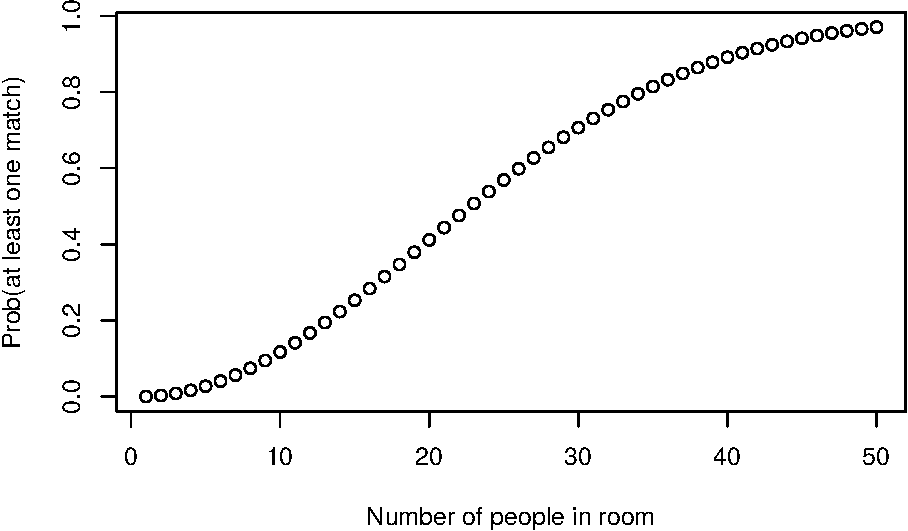
\includegraphics{_main_files/figure-latex/birthday-1.pdf}
\caption{\label{fig:birthday}\small The birthday problem. The horizontal line is
at \(p=0.50\) and the vertical line is at \(n=23\).}
\end{figure}




\subsubsection{How to do it with R}\label{how-to-do-it-with-r-14}

We can make the plot in Figure \ref{fig:birthday} with the following
sequence of commands.

\begin{Shaded}
\begin{Highlighting}[]
\KeywordTok{library}\NormalTok{(RcmdrPlugin.IPSUR)}
\NormalTok{g <-}\StringTok{ }\KeywordTok{Vectorize}\NormalTok{(pbirthday.ipsur)}
\KeywordTok{plot}\NormalTok{(}\DecValTok{1}\NormalTok{:}\DecValTok{50}\NormalTok{, }\KeywordTok{g}\NormalTok{(}\DecValTok{1}\NormalTok{:}\DecValTok{50}\NormalTok{), }\DataTypeTok{xlab =} \StringTok{"Number of people in room"}\NormalTok{, }
  \DataTypeTok{ylab =} \StringTok{"Prob(at least one match)"} \NormalTok{)}
\KeywordTok{abline}\NormalTok{(}\DataTypeTok{h =} \FloatTok{0.5}\NormalTok{)}
\KeywordTok{abline}\NormalTok{(}\DataTypeTok{v =} \DecValTok{23}\NormalTok{, }\DataTypeTok{lty =} \DecValTok{2}\NormalTok{)}
\KeywordTok{remove}\NormalTok{(g)}
\end{Highlighting}
\end{Shaded}

There is a \texttt{Birthday\ problem} item in the \texttt{Probability}
menu of \texttt{RcmdrPlugin.IPSUR}. In the base R version, one can
compute approximate probabilities for the more general case of
probabilities other than 1/2, for differing total number of days in the
year, and even for more than two matches.

\section{Conditional Probability}\label{sec-conditional-probability}

Consider a full deck of 52 standard playing cards. Now select two cards
from the deck, in succession. Let
\(A = \{ \mbox{first card drawn is an Ace} \}\) and
\(B = \{ \mbox{second card drawn is an Ace} \}\). Since there are four
Aces in the deck, it is natural to assign \(\mathbb{P}(A) = 4/52\).
Suppose we look at the first card. What now is the probability of \(B\)?
Of course, the answer depends on the value of the first card. If the
first card is an Ace, then the probability that the second also is an
Ace should be \(3/51\), but if the first card is not an Ace, then the
probability that the second is an Ace should be \(4/51\). As notation
for these two situations we write \[ 
\mathbb{P}(B\vert A)=3/51,\quad
\mathbb{P}(B\vert A^{c})=4/51.  
\]

\bigskip

\BeginKnitrBlock{definition}
\protect\hypertarget{def:unnamed-chunk-151}{}{\label{def:unnamed-chunk-151}}The
conditional probability of \(B\) given \(A\), denoted
\(\mathbb{P}(B|A)\), is defined by

\begin{equation}
\mathbb{P}(B|A)=\frac{\mathbb{P}(A\cap B)}{\mathbb{P}(A)},\quad \mbox{if }\mathbb{P}(A)>0.
\end{equation}
\EndKnitrBlock{definition}

We will not be discussing a conditional probability of \(B\) given \(A\)
when \(\mathbb{P}(A)=0\), even though this theory exists, is well
developed, and forms the foundation for the study of stochastic
processes\footnote{In other words, a variable might be highly
  significant one moment but then fail to be significant when another
  variable is added to the model. When this happens it often indicates a
  problem with the explanatory variables, such as
  \emph{multicollinearity}. See Section \ref{sub-Multicollinearity}.}.

Toss a coin twice. The sample space is given by \(S=\{ HH,\ HT,\ TH,\
TT \}\). Let \(A= \{ \mbox{a head occurs} \}\) and
\(B= \{ \mbox{a head and tail occur} \}\). It should be clear that
\(\mathbb{P}(A)=3/4\), \(\mathbb{P}(B)=2/4\), and
\(\mathbb{P}(A\cap B)=2/4\). What now are the probabilities
\(\mathbb{P}(A|B)\) and \(\mathbb{P}(B|A)\)?

\[ \mathbb{P}(A|B)=\frac{\mathbb{P}(A\cap
B)}{\mathbb{P}(B)}=\frac{2/4}{2/4}=1, \]

in other words, once we know that a Head and Tail occur, we may be
certain that a Head occurs. Next

\[ 
\mathbb{P}(B|A)=\frac{\mathbb{P}(A\cap
B)}{\mathbb{P}(A)}=\frac{2/4}{3/4}=\frac{2}{3}, 
\]

which means that given the information that a Head has occurred, we no
longer need to account for the outcome \(TT\), and the remaining three
outcomes are equally likely with exactly two outcomes lying in the set
\(B\).

\bigskip

\BeginKnitrBlock{example}
\protect\hypertarget{ex:toss-a-six-sided-die-twice}{}{\label{ex:toss-a-six-sided-die-twice}}Toss
a six-sided die twice. The sample space consists of all ordered pairs
\((i,j)\) of the numbers \(1,2,\ldots,6\), that is,
\(S = \{ (1,1),\ (1,2),\ldots,(6,6) \} \). We know from Section
\ref{sec-methods-of-counting} that \(\# (S) = 6^{2} = 36\). Let
\(A = \{ \mbox{outcomes match} \}\) and
\(B = \{ \mbox{sum of outcomes at least 8} \}\). The sample space may be
represented by a matrix:
\EndKnitrBlock{example}

\begin{figure}[htbp]
\centering
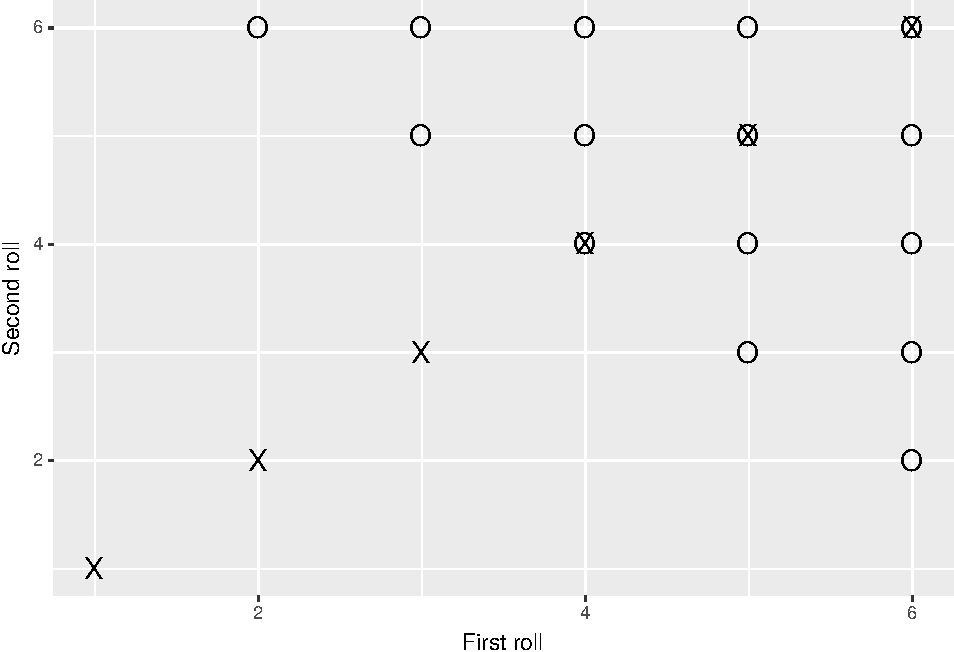
\includegraphics{_main_files/figure-latex/twodiceAB-1.pdf}
\caption{\label{fig:twodiceAB}\small Rolling two dice. The outcomes in A are
marked with X, the outcomes in B are marked with O.}
\end{figure}




The outcomes lying in the event \(A\) are marked with the symbol ``X'',
the outcomes falling in \(B\) are marked with ``O'', and the outcomes in
\(A\cap B\) are those where the letters overlap. Now it is clear that
\(\mathbb{P}(A)=6/36\), \(\mathbb{P}(B)=15/36\), and
\(\mathbb{P}(A\cap B)=3/36\). Finally, \[
\mathbb{P}(A|B)=\frac{3/36}{15/36}=\frac{1}{5},\quad
\mathbb{P}(B|A)=\frac{3/36}{6/36}=\frac{1}{2}.  
\] Again, we see that given the knowledge that \(B\) occurred (the 15
outcomes in the upper right triangle), there are 3 of the 15 that fall
into the set \(A\), thus the probability is \(3/15\). Similarly, given
that \(A\) occurred (we are on the diagonal), there are 3 out of 6
outcomes that also fall in \(B\), thus, the probability of \(B\) given
\(A\) is 1/2.

\subsection{How to do it with R}\label{how-to-do-it-with-r-15}

Continuing with Example \ref{ex:toss-a-six-sided-die-twice}, the first
thing to do is set up the probability space with the \texttt{rolldie}
function.

\begin{Shaded}
\begin{Highlighting}[]
\NormalTok{S <-}\StringTok{ }\KeywordTok{rolldie}\NormalTok{(}\DecValTok{2}\NormalTok{, }\DataTypeTok{makespace =} \OtherTok{TRUE}\NormalTok{)  }\CommentTok{# assumes ELM}
\KeywordTok{head}\NormalTok{(S)                            }\CommentTok{#  first few rows}
\end{Highlighting}
\end{Shaded}

\begin{verbatim}
  X1 X2      probs
1  1  1 0.02777778
2  2  1 0.02777778
3  3  1 0.02777778
4  4  1 0.02777778
5  5  1 0.02777778
6  6  1 0.02777778
\end{verbatim}

Next we define the events

\begin{Shaded}
\begin{Highlighting}[]
\NormalTok{A <-}\StringTok{ }\KeywordTok{subset}\NormalTok{(S, X1 ==}\StringTok{ }\NormalTok{X2)}
\NormalTok{B <-}\StringTok{ }\KeywordTok{subset}\NormalTok{(S, X1 +}\StringTok{ }\NormalTok{X2 >=}\StringTok{ }\DecValTok{8}\NormalTok{)}
\end{Highlighting}
\end{Shaded}

And now we are ready to calculate probabilities. To do conditional
probability, we use the \texttt{given} argument of the \texttt{Prob}
function:

\begin{Shaded}
\begin{Highlighting}[]
\KeywordTok{Prob}\NormalTok{(A, }\DataTypeTok{given =} \NormalTok{B)}
\end{Highlighting}
\end{Shaded}

\begin{verbatim}
[1] 0.2
\end{verbatim}

\begin{Shaded}
\begin{Highlighting}[]
\KeywordTok{Prob}\NormalTok{(B, }\DataTypeTok{given =} \NormalTok{A)}
\end{Highlighting}
\end{Shaded}

\begin{verbatim}
[1] 0.5
\end{verbatim}

Note that we do not actually need to define the events \(A\) and \(B\)
separately as long as we reference the original probability space \(S\)
as the first argument of the \texttt{Prob} calculation:

\begin{Shaded}
\begin{Highlighting}[]
\KeywordTok{Prob}\NormalTok{(S, X1==X2, }\DataTypeTok{given =} \NormalTok{(X1 +}\StringTok{ }\NormalTok{X2 >=}\StringTok{ }\DecValTok{8}\NormalTok{) )}
\end{Highlighting}
\end{Shaded}

\begin{verbatim}
[1] 0.2
\end{verbatim}

\begin{Shaded}
\begin{Highlighting}[]
\KeywordTok{Prob}\NormalTok{(S, X1+X2 >=}\StringTok{ }\DecValTok{8}\NormalTok{, }\DataTypeTok{given =} \NormalTok{(X1==X2) )}
\end{Highlighting}
\end{Shaded}

\begin{verbatim}
[1] 0.5
\end{verbatim}

\subsection{Properties and Rules}\label{properties-and-rules}

The following theorem establishes that conditional probabilities behave
just like regular probabilities when the conditioned event is fixed.

\bigskip

\BeginKnitrBlock{theorem}
\protect\hypertarget{thm:unnamed-chunk-156}{}{\label{thm:unnamed-chunk-156}}For
any fixed event \(A\) with \(\mathbb{P}(A)>0\),

\begin{enumerate}
\def\labelenumi{\arabic{enumi}.}
\tightlist
\item
  \(\mathbb{P} (B|A)\geq 0\), for all events \(B \subset S\),
\item
  \(\mathbb{P} (S|A) = 1\), and
\item
  If \(B_{1}\), \(B_{2}\), \(B_{3}\),\ldots{} are disjoint events, then

  \begin{equation}
    \mathbb{P}\left(\left.\bigcup_{k=1}^{\infty}B_{k}\:\right|A\right)=\sum_{k=1}^{\infty}\mathbb{P}(B_{k}|A).
    \end{equation}
\end{enumerate}
\EndKnitrBlock{theorem}

In other words, \(\mathbb{P}(\cdot|A)\) is a legitimate probability
function. With this fact in mind, the following properties are
immediate:

\bigskip

\BeginKnitrBlock{proposition}
\protect\hypertarget{prp:unnamed-chunk-157}{}{\label{prp:unnamed-chunk-157}}For
any events \(A\), \(B\), and \(C\) with \(\mathbb{P}(A)>0\),

\begin{enumerate}
\def\labelenumi{\arabic{enumi}.}
\tightlist
\item
  \(\mathbb{P} ( B^{c} | A ) = 1 - \mathbb{P} (B|A).\)
\item
  If \(B\subset C\) then \(\mathbb{P}(B|A)\leq\mathbb{P}(C|A)\).
\item
  \(\mathbb{P} [ ( B\cup C ) | A ] = \mathbb{P} (B|A) +  \mathbb{P}(C|A) - \mathbb{P} [ (B \cap C|A) ].\)
\item
  \textbf{The Multiplication Rule.} For any two events \(A\) and \(B\),

  \begin{equation}
     \label{eq-multiplication-rule-short}
     \mathbb{P}(A\cap B)=\mathbb{P}(A)\mathbb{P}(B|A).
     \end{equation}

  And more generally, for events \(A_{1}\), \(A_{2}\),
  \(A_{3}\),\ldots{}, \(A_{n}\),

  \begin{equation}
     \label{eq-multiplication-rule-long}
     \mathbb{P}(A_{1}\cap A_{2}\cap\cdots\cap A_{n})=\mathbb{P}(A_{1})\mathbb{P}(A_{2}|A_{1})\cdots\mathbb{P}(A_{n}|A_{1}\cap A_{2}\cap\cdots\cap A_{n-1}).
     \end{equation}
\end{enumerate}
\EndKnitrBlock{proposition}

The Multiplication Rule is very important because it allows us to find
probabilities in random experiments that have a sequential structure, as
the next example shows.

\bigskip

\BeginKnitrBlock{example}
\protect\hypertarget{ex:two-cards-both-aces}{}{\label{ex:two-cards-both-aces}}At
the beginning of the section we drew two cards from a standard playing
deck. Now we may answer our original question, what is
\(\mathbb{P}(\mbox{both Aces})\)? \[
\mathbb{P}(\mbox{both Aces})=\mathbb{P}(A\cap
B)=\mathbb{P}(A)\mathbb{P}(B|A)=\frac{4}{52}\cdot\frac{3}{51}\approx0.00452.
\]
\EndKnitrBlock{example}

\subsubsection{How to do it with R}\label{sub-howto-ps-objects}

Continuing Example \ref{ex:two-cards-both-aces}, we set up the
probability space by way of a three step process. First we employ the
\texttt{cards} function to get a data frame \texttt{L} with two columns:
\texttt{rank} and \texttt{suit}. Both columns are stored internally as
factors with 13 and 4 levels, respectively.

Next we sample two cards randomly from the \texttt{L} data frame by way
of the \texttt{urnsamples} function. It returns a list \texttt{M} which
contains all possible pairs of rows from \texttt{L} (there are
\texttt{choose(52,2)} of them). The sample space for this experiment is
exactly the list \texttt{M}.

At long last we associate a probability model with the sample space.
This is right down the \texttt{probspace} function's alley. It assumes
the equally likely model by default. We call this result \texttt{N}
which is an object of class \texttt{ps} -- short for ``probability
space''.

But do not be intimidated. The object \texttt{N} is nothing more than a
list with two elements: \texttt{outcomes} and \texttt{probs}. The
\texttt{outcomes} element is itself just another list, with
\texttt{choose(52,2)} entries, each one a data frame with two rows which
correspond to the pair of cards chosen. The \texttt{probs} element is
just a vector with \texttt{choose(52,2)} entries all the same:
\texttt{1/choose(52,2)}.

Putting all of this together we do

\begin{Shaded}
\begin{Highlighting}[]
\NormalTok{L <-}\StringTok{ }\KeywordTok{cards}\NormalTok{()}
\NormalTok{M <-}\StringTok{ }\KeywordTok{urnsamples}\NormalTok{(L, }\DataTypeTok{size =} \DecValTok{2}\NormalTok{)}
\NormalTok{N <-}\StringTok{ }\KeywordTok{probspace}\NormalTok{(M)}
\NormalTok{N[[}\DecValTok{1}\NormalTok{]][[}\DecValTok{1}\NormalTok{]];  N$probs[}\DecValTok{1}\NormalTok{]}
\end{Highlighting}
\end{Shaded}

\begin{verbatim}
  rank suit
1    2 Club
2    3 Club
\end{verbatim}

\begin{verbatim}
[1] 0.0007541478
\end{verbatim}

Now that we have the probability space \texttt{N} we are ready to do
some probability. We use the \texttt{Prob} function, just like before.
The only trick is to specify the event of interest correctly, and recall
that we were interested in \(\mathbb{P}(\mbox{both Aces})\). But if the
cards are both Aces then the \texttt{rank} of both cards should be
\texttt{A}, which sounds like a job for the \texttt{all} function:

\begin{Shaded}
\begin{Highlighting}[]
\KeywordTok{Prob}\NormalTok{(N, }\KeywordTok{all}\NormalTok{(rank ==}\StringTok{ "A"}\NormalTok{))}
\end{Highlighting}
\end{Shaded}

\begin{verbatim}
[1] 0.004524887
\end{verbatim}

Note that this value matches what we found in Example
\ref{ex:two-cards-both-aces}, above. We could calculate all sorts of
probabilities at this point; we are limited only by the complexity of
the event's computer representation.

\bigskip

\BeginKnitrBlock{example}
\protect\hypertarget{ex:urn-7-red-3-green}{}{\label{ex:urn-7-red-3-green}}Consider
an urn with 10 balls inside, 7 of which are red and 3 of which are
green. Select 3 balls successively from the urn. Let
\(A = \{ 1^{\mathrm{st}} \mbox{ ball is red} \}\),
\(B = \{ 2^{\mathrm{nd}} \mbox{ ball is red} \}\), and
\(C = \{ 3^{\mathrm{rd}} \mbox{ ball is red} \}\). Then \[
\mathbb{P}(\mbox{all 3 balls are red})=\mathbb{P}(A\cap B\cap
C)=\frac{7}{10}\cdot\frac{6}{9}\cdot\frac{5}{8}\approx 0.2917.  \]
\EndKnitrBlock{example}

\subsubsection{How to do it with R}\label{how-to-do-it-with-r-16}

Example \ref{ex:urn-7-red-3-green} is similar to Example
\ref{ex:two-cards-both-aces}, but it is even easier. We need to set up
an urn (vector \texttt{L}) to hold the balls, we sample from \texttt{L}
to get the sample space (data frame \texttt{M}), and we associate a
probability vector (column \texttt{probs}) with the outcomes (rows of
\texttt{M}) of the sample space. The final result is a probability space
(an ordinary data frame \texttt{N}).

It is easier for us this time because our urn is a vector instead of a
\texttt{cards()} data frame. Before there were two dimensions of
information associated with the outcomes (rank and suit) but presently
we have only one dimension (color).

\begin{Shaded}
\begin{Highlighting}[]
\NormalTok{L <-}\StringTok{ }\KeywordTok{rep}\NormalTok{(}\KeywordTok{c}\NormalTok{(}\StringTok{"red"}\NormalTok{,}\StringTok{"green"}\NormalTok{), }\DataTypeTok{times =} \KeywordTok{c}\NormalTok{(}\DecValTok{7}\NormalTok{,}\DecValTok{3}\NormalTok{))}
\NormalTok{M <-}\StringTok{ }\KeywordTok{urnsamples}\NormalTok{(L, }\DataTypeTok{size =} \DecValTok{3}\NormalTok{, }\DataTypeTok{replace =} \OtherTok{FALSE}\NormalTok{, }\DataTypeTok{ordered =} \OtherTok{TRUE}\NormalTok{)}
\NormalTok{N <-}\StringTok{ }\KeywordTok{probspace}\NormalTok{(M)}
\end{Highlighting}
\end{Shaded}

Now let us think about how to set up the event
\(\{ \mbox{all 3 balls are red}\}\). Rows of \texttt{N} that satisfy
this condition have \texttt{X1=="red"\ \&\ X2=="red"\ \&\ X3=="red"},
but there must be an easier way. Indeed, there is. The \texttt{isrep}
function (short for ``is repeated'') in the \texttt{prob} package was
written for this purpose. The command \texttt{isrep(N,"red",3)} will
test each row of \texttt{N} to see whether the value \texttt{red}
appears \texttt{3} times. The result is exactly what we need to define
an event with the \texttt{Prob} function. Observe

\begin{Shaded}
\begin{Highlighting}[]
\KeywordTok{Prob}\NormalTok{(N, }\KeywordTok{isrep}\NormalTok{(N, }\StringTok{"red"}\NormalTok{, }\DecValTok{3}\NormalTok{))}
\end{Highlighting}
\end{Shaded}

\begin{verbatim}
[1] 0.2916667
\end{verbatim}

Note that this answer matches what we found in Example
\ref{ex:urn-7-red-3-green}. Now let us try some other probability
questions. What is the probability of getting two \texttt{red}'s?

\begin{Shaded}
\begin{Highlighting}[]
\KeywordTok{Prob}\NormalTok{(N, }\KeywordTok{isrep}\NormalTok{(N, }\StringTok{"red"}\NormalTok{, }\DecValTok{2}\NormalTok{))}
\end{Highlighting}
\end{Shaded}

\begin{verbatim}
[1] 0.525
\end{verbatim}

Note that the exact value is \(21/40\); we will learn a quick way to
compute this in Section \ref{sec-other-discrete-distributions}. What is
the probability of observing \texttt{red}, then \texttt{green}, then
\texttt{red}?

\begin{Shaded}
\begin{Highlighting}[]
\KeywordTok{Prob}\NormalTok{(N, }\KeywordTok{isin}\NormalTok{(N, }\KeywordTok{c}\NormalTok{(}\StringTok{"red"}\NormalTok{,}\StringTok{"green"}\NormalTok{,}\StringTok{"red"}\NormalTok{), }\DataTypeTok{ordered =} \OtherTok{TRUE}\NormalTok{))}
\end{Highlighting}
\end{Shaded}

\begin{verbatim}
[1] 0.175
\end{verbatim}

Note that the exact value is \(7/40\) (do it with the Multiplication
Rule). What is the probability of observing \texttt{red},
\texttt{green}, and \texttt{red}, in no particular order?

\begin{Shaded}
\begin{Highlighting}[]
\KeywordTok{Prob}\NormalTok{(N, }\KeywordTok{isin}\NormalTok{(N, }\KeywordTok{c}\NormalTok{(}\StringTok{"red"}\NormalTok{,}\StringTok{"green"}\NormalTok{,}\StringTok{"red"}\NormalTok{)))}
\end{Highlighting}
\end{Shaded}

\begin{verbatim}
[1] 0.525
\end{verbatim}

We already knew this. It is the probability of observing two
\texttt{red}'s, above.

\bigskip

\BeginKnitrBlock{example}
\protect\hypertarget{ex:unnamed-chunk-165}{}{\label{ex:unnamed-chunk-165}}Consider
two urns, the first with 5 red balls and 3 green balls, and the second
with 2 red balls and 6 green balls. Your friend randomly selects one
ball from the first urn and transfers it to the second urn, without
disclosing the color of the ball. You select one ball from the second
urn. What is the probability that the selected ball is red?
\EndKnitrBlock{example}

Let \(A = \{ \mbox{transferred ball is red} \}\) and
\(B = \{ \mbox{selected ball is red} \}\). Write

\begin{align*}
B & =S\cap B\\
 & =(A\cup A^{c})\cap B\\
 & =(A\cap B)\cup(A^{c}\cap B)
\end{align*}

and notice that \(A\cap B\) and \(A^{c}\cap B\) are disjoint. Therefore

\begin{align*}
\mathbb{P}(B) & =\mathbb{P}(A\cap B)+\mathbb{P}(A^{c}\cap B)\\
 & =\mathbb{P}(A)\mathbb{P}(B|A)+\mathbb{P}(A^{c})\mathbb{P}(B|A^{c})\\
 & =\frac{5}{8}\cdot\frac{3}{9}+\frac{3}{8}\cdot\frac{2}{9}\\
 & =\frac{21}{72}\ 
\end{align*}

(which is 7/24 in lowest terms).

\bigskip

\BeginKnitrBlock{example}
\protect\hypertarget{ex:unnamed-chunk-166}{}{\label{ex:unnamed-chunk-166}}We
saw the \texttt{RcmdrTestDrive} data set in Chapter
\ref{cha-introduction-to-R} in which a two-way table of the smoking
status versus the gender was
\EndKnitrBlock{example}

\begin{Shaded}
\begin{Highlighting}[]
\KeywordTok{library}\NormalTok{(RcmdrPlugin.IPSUR)}
\KeywordTok{data}\NormalTok{(RcmdrTestDrive)  }
\NormalTok{.Table <-}\StringTok{ }\KeywordTok{xtabs}\NormalTok{( ~}\StringTok{ }\NormalTok{smoking +}\StringTok{ }\NormalTok{gender, }\DataTypeTok{data =} \NormalTok{RcmdrTestDrive)}
\KeywordTok{addmargins}\NormalTok{(.Table) }\CommentTok{# Table with marginal distributions}
\end{Highlighting}
\end{Shaded}

\begin{verbatim}
           gender
smoking     Female Male Sum
  Nonsmoker     61   75 136
  Smoker         9   23  32
  Sum           70   98 168
\end{verbatim}

If one person were selected at random from the data set, then we see
from the two-way table that \(\mathbb{P}(\mbox{Female})=70/168\) and
\(\mathbb{P}(\mbox{Smoker})=32/168\). Now suppose that one of the
subjects quits smoking, but we do not know the person's gender. If we
now select one nonsmoker at random, what would be
\(\mathbb{P}(\mbox{Female})\)? This example is just like the last
example, but with different labels. Let
\(A = \{ \mbox{the quitter is a female} \}\) and
\(B = \{ \mbox{selected nonsmoker is a female} \} \). Write

\begin{align*}
B & =S\cap B\\
 & =(A\cup A^{c})\cap B\\
 & =(A\cap B)\cup(A^{c}\cap B)
\end{align*}

and notice that \(A\cap B\) and \(A^{c}\cap B\) are disjoint. Therefore

\begin{align*}
\mathbb{P}(B) & =\mathbb{P}(A\cap B)+\mathbb{P}(A^{c}\cap B),\\
 & =\mathbb{P}(A)\mathbb{P}(B|A)+\mathbb{P}(A^{c})\mathbb{P}(B|A^{c}),\\
 & =\frac{9}{32}\cdot\frac{62}{137}+\frac{23}{32}\cdot\frac{76}{137},\\
 & =\frac{2306}{4384},
\end{align*}

(which is 1153/2192 in lowest terms).

Using the same reasoning, we can return to the example from the
beginning of the section and show that \[ \mathbb{P}(\{ \mbox{second
card is an Ace} \} )=4/52.
\]

\section{Independent Events}\label{sec-independent-events}

Toss a coin twice. The sample space is \(S= \{ HH,\ HT,\ TH,\ TT \} \).
We know that \(\mathbb{P}(1^{\mathrm{st}}\mbox{ toss is }H)=2/4\),
\(\mathbb{P}(2^{\mathrm{nd}}\mbox{ toss is }H)=2/4\), and
\(\mathbb{P}(\mbox{both }H)=1/4\). Then

\begin{align*} 
\mathbb{P}(2^{\mathrm{nd}}\mbox{ toss is }H\ \vert \ 1^{\mathrm{st}}\mbox{ toss is }H) & =\frac{\mathbb{P}(\mbox{both }H)}{\mathbb{P}(1^{\mathrm{st}}\mbox{ toss is }H)}, \\
 & =\frac{1/4}{2/4},\\
 & =\mathbb{P}(2^{\mathrm{nd}}\mbox{ toss is }H).
\end{align*}

Intuitively, this means that the information that the first toss is
\(H\) has no bearing on the probability that the second toss is \(H\).
The coin does not remember the result of the first toss.

\bigskip

\BeginKnitrBlock{definition}
\protect\hypertarget{def:unnamed-chunk-168}{}{\label{def:unnamed-chunk-168}}Events
\(A\) and \(B\) are said to be \emph{independent} if

\begin{equation}
\mathbb{P}(A\cap B)=\mathbb{P}(A)\mathbb{P}(B).
\end{equation}

Otherwise, the events are said to be \emph{dependent}.
\EndKnitrBlock{definition}

The connection with the above example stems from the following. We know
from Section \ref{sec-conditional-probability} that when
\(\mathbb{P}(B)>0\) we may write

\begin{equation}
\mathbb{P}(A|B)=\frac{\mathbb{P}(A\cap B)}{\mathbb{P}(B)}.
\end{equation}

In the case that \(A\) and \(B\) are independent, the numerator of the
fraction factors so that \(\mathbb{P}(B)\) cancels with the result:

\begin{equation}
\mathbb{P}(A|B)=\mathbb{P}(A)\mbox{ when \(A\), \(B\) are independent.}
\end{equation}

The interpretation in the case of independence is that the information
that the event \(B\) occurred does not influence the probability of the
event \(A\) occurring. Similarly, \(\mathbb{P}(B|A)=\mathbb{P}(B)\), and
so the occurrence of the event \(A\) likewise does not affect the
probability of event \(B\). It may seem more natural to define \(A\) and
\(B\) to be independent when \(\mathbb{P}(A|B)=\mathbb{P}(A)\); however,
the conditional probability \(\mathbb{P}(A|B)\) is only defined when
\(\mathbb{P}(B)>0\). Our definition is not limited by this restriction.
It can be shown that when \(\mathbb{P}(A),\
\mathbb{P}(B)>0\) the two notions of independence are equivalent.

\bigskip

\BeginKnitrBlock{proposition}
\protect\hypertarget{prp:unnamed-chunk-169}{}{\label{prp:unnamed-chunk-169}}If
the events \(A\) and \(B\) are independent then

\begin{itemize}
\tightlist
\item
  \(A\) and \(B^{c}\) are independent,
\item
  \(A^{c}\) and \(B\) are independent,
\item
  \(A^{c}\) and \(B^{c}\) are independent.
\end{itemize}
\EndKnitrBlock{proposition}

\BeginKnitrBlock{proof}
\iffalse {Proof. } \fi Suppose that \(A\) and \(B\) are independent. We
will show the second one; the others are similar. We need to show that
\[
\mathbb{P}(A^{c}\cap B)=\mathbb{P}(A^{c})\mathbb{P}(B).  \] To this end,
note that the Multiplication Rule, Equation
\eqref{eq-multiplication-rule-short} implies

\begin{eqnarray*}
\mathbb{P}(A^{c}\cap B) & = & \mathbb{P}(B)\mathbb{P}(A^{c}|B),\\
 & = & \mathbb{P}(B)[1-\mathbb{P}(A|B)],\\
 & = & \mathbb{P}(B)\mathbb{P}(A^{c}).
\end{eqnarray*}
\EndKnitrBlock{proof}

\bigskip

\BeginKnitrBlock{definition}
\protect\hypertarget{def:unnamed-chunk-171}{}{\label{def:unnamed-chunk-171}}The
events \(A\), \(B\), and \(C\) are \emph{mutually independent} if the
following four conditions are met:

\begin{eqnarray*}
\mathbb{P}(A\cap B) & = & \mathbb{P}(A)\mathbb{P}(B),\\
\mathbb{P}(A\cap C) & = & \mathbb{P}(A)\mathbb{P}(C),\\
\mathbb{P}(B\cap C) & = & \mathbb{P}(B)\mathbb{P}(C),
\end{eqnarray*}

and \[
\mathbb{P}(A\cap B\cap C)=\mathbb{P}(A)\mathbb{P}(B)\mathbb{P}(C).
\] If only the first three conditions hold then \(A\), \(B\), and \(C\)
are said to be independent \emph{pairwise}. Note that pairwise
independence is not the same as mutual independence when the number of
events is larger than two.
\EndKnitrBlock{definition}

We can now deduce the pattern for \(n\) events, \(n>3\). The events will
be mutually independent only if they satisfy the product equality
pairwise, then in groups of three, in groups of four, and so forth, up
to all \(n\) events at once. For \(n\) events, there will be
\(2^{n}-n-1\) equations that must be satisfied (see Exercise
\ref{xca-numb-cond-indep}). Although these requirements for a set of
events to be mutually independent may seem stringent, the good news is
that for most of the situations considered in this book the conditions
will all be met (or at least we will suppose that they are).

\bigskip

\BeginKnitrBlock{example}
\protect\hypertarget{ex:toss-ten-coins}{}{\label{ex:toss-ten-coins}}Toss ten
coins. What is the probability of observing at least one Head?
\EndKnitrBlock{example}

\textbf{Answer:} Let
\(A_{i}= \{ \mbox{the }i^{\mathrm{th}}\mbox{ coin shows }H \} ,\
i=1,2,\ldots,10\). Supposing that we toss the coins in such a way that
they do not interfere with each other, this is one of the situations
where all of the \(A_{i}\) may be considered mutually independent due to
the nature of the tossing. Of course, the only way that there will not
be at least one Head showing is if all tosses are Tails. Therefore,

\begin{align*}
\mathbb{P}(\mbox{at least one }H) & =1-\mathbb{P}(\mbox{all }T),\\
 & =1-\mathbb{P}(A_{1}^{c}\cap A_{2}^{c}\cap\cdots\cap A_{10}^{c}),\\
 & =1-\mathbb{P}(A_{1}^{c})\mathbb{P}(A_{2}^{c})\cdots\mathbb{P}(A_{10}^{c}),\\
 & =1-\left(\frac{1}{2}\right)^{10},
\end{align*}

which is approximately \(0.9990234\).

\subsection{How to do it with R}\label{how-to-do-it-with-r-17}

\BeginKnitrBlock{example}
\protect\hypertarget{ex:unnamed-chunk-172}{}{\label{ex:unnamed-chunk-172}}Toss
ten coins. What is the probability of observing at least one Head?
\EndKnitrBlock{example}

\begin{Shaded}
\begin{Highlighting}[]
\NormalTok{S <-}\StringTok{ }\KeywordTok{tosscoin}\NormalTok{(}\DecValTok{10}\NormalTok{, }\DataTypeTok{makespace =} \OtherTok{TRUE}\NormalTok{)}
\NormalTok{A <-}\StringTok{ }\KeywordTok{subset}\NormalTok{(S, }\KeywordTok{isrep}\NormalTok{(S, }\DataTypeTok{vals =} \StringTok{"T"}\NormalTok{, }\DataTypeTok{nrep =} \DecValTok{10}\NormalTok{))}
\DecValTok{1} \NormalTok{-}\StringTok{ }\KeywordTok{Prob}\NormalTok{(A)}
\end{Highlighting}
\end{Shaded}

\begin{verbatim}
[1] 0.9990234
\end{verbatim}

Compare this answer to what we got in Example \ref{ex:toss-ten-coins}.

\subsection{Independent, Repeated
Experiments}\label{independent-repeated-experiments}

Generalizing from above it is common to repeat a certain experiment
multiple times under identical conditions and in an independent manner.
We have seen many examples of this already: tossing a coin repeatedly,
rolling a die or dice, \emph{etc}.

The \texttt{iidspace} function was designed specifically for this
situation. It has three arguments: \texttt{x}, which is a vector of
outcomes, \texttt{ntrials}, which is an integer telling how many times
to repeat the experiment, and \texttt{probs} to specify the
probabilities of the outcomes of \texttt{x} in a single trial.

\bigskip

\BeginKnitrBlock{example}[An unbalanced coin]
\protect\hypertarget{ex:unnamed-chunk-174}{}{\label{ex:unnamed-chunk-174}
\iffalse (An unbalanced coin) \fi }(Continued, see Example
\ref{ex:unbalanced-coin}). It was easy enough to set up the probability
space for one unbalanced toss, however, the situation becomes more
complicated when there are many tosses involved. Clearly, the outcome
\(HHH\) should not have the same probability as \(TTT\), which should
again not have the same probability as \(HTH\). At the same time, there
is symmetry in the experiment in that the coin does not remember the
face it shows from toss to toss, and it is easy enough to toss the coin
in a similar way repeatedly.
\EndKnitrBlock{example}

We may represent tossing our unbalanced coin three times with the
following:

\begin{Shaded}
\begin{Highlighting}[]
\KeywordTok{iidspace}\NormalTok{(}\KeywordTok{c}\NormalTok{(}\StringTok{"H"}\NormalTok{,}\StringTok{"T"}\NormalTok{), }\DataTypeTok{ntrials =} \DecValTok{3}\NormalTok{, }\DataTypeTok{probs =} \KeywordTok{c}\NormalTok{(}\FloatTok{0.7}\NormalTok{, }\FloatTok{0.3}\NormalTok{)) }
\end{Highlighting}
\end{Shaded}

\begin{verbatim}
  X1 X2 X3 probs
1  H  H  H 0.343
2  T  H  H 0.147
3  H  T  H 0.147
4  T  T  H 0.063
5  H  H  T 0.147
6  T  H  T 0.063
7  H  T  T 0.063
8  T  T  T 0.027
\end{verbatim}

As expected, the outcome \(HHH\) has the largest probability, while
\(TTT\) has the smallest. (Since the trials are independent,
\(\mathbb{P}(HHH)=0.7^{3}\) and \(\mathbb{P}(TTT)=0.3^{3}\),
\emph{etc}.) Note that the result of the function call is a probability
space, not a sample space (which we could construct already with the
\texttt{tosscoin} or \texttt{urnsamples} functions). The same procedure
could be used to model an unbalanced die or any other experiment that
may be represented with a vector of possible outcomes.

Note that \texttt{iidspace} will assume \texttt{x} has equally likely
outcomes if no \texttt{probs} argument is specified. Also note that the
argument \texttt{x} is a \emph{vector}, not a data frame. Something like
: iidspace(tosscoin(1),\ldots{}) would give an error.

\section{Bayes' Rule}\label{sec-bayes-rule}

We mentioned the subjective view of probability in Section
\ref{sec-interpreting-probabilities}. In this section we introduce a
rule that allows us to update our probabilities when new information
becomes available.

\bigskip

\BeginKnitrBlock{theorem}[Bayes' Rule]
\protect\hypertarget{thm:unnamed-chunk-176}{}{\label{thm:unnamed-chunk-176}
\iffalse (Bayes' Rule) \fi }Let \(B_{1}\), \(B_{2}\), \ldots{},
\(B_{n}\) be mutually exclusive and exhaustive and let \(A\) be an event
with \(\mathbb{P}(A)>0\). Then

\begin{equation}
\label{eq-bayes-rule}
\mathbb{P}(B_{k}|A)=\frac{\mathbb{P}(B_{k})\mathbb{P}(A|B_{k})}{\sum_{i=1}^{n}\mathbb{P}(B_{i})\mathbb{P}(A|B_{i})},\quad k=1,2,\ldots,n.
\end{equation}
\EndKnitrBlock{theorem}

\BeginKnitrBlock{proof}
\iffalse {Proof. } \fi The proof follows from looking at
\(\mathbb{P}(B_{k}\cap A)\) in two different ways. For simplicity,
suppose that \(P(B_{k})>0\) for all \(k\). Then
\[ \mathbb{P}(A)\mathbb{P}(B_{k}|A)=\mathbb{P}(B_{k}\cap
A)=\mathbb{P}(B_{k})\mathbb{P}(A|B_{k}).  \] Since \(\mathbb{P}(A)>0\)
we may divide through to obtain \[
\mathbb{P}(B_{k}|A)=\frac{\mathbb{P}(B_{k})\mathbb{P}(A|B_{k})}{\mathbb{P}(A)}.
\] Now remembering that \(\{ B_{k} \}\) is a partition, the Theorem of
Total Probability (Equation \eqref{eq-theorem-total-probability} ) gives
the denominator of the last expression to be \[
\mathbb{P}(A)=\sum_{k=1}^{n}\mathbb{P}(B_{k}\cap
A)=\sum_{k=1}^{n}\mathbb{P}(B_{k})\mathbb{P}(A|B_{k}).  \]
\EndKnitrBlock{proof}

What does it mean? Usually in applications we are given (or know)
\emph{a priori} probabilities \(\mathbb{P}(B_{k})\). We go out and
collect some data, which we represent by the event \(A\). We want to
know: how do we \emph{update} \(\mathbb{P}(B_{k})\) to
\(\mathbb{P}(B_{k}|A)\)? The answer: Bayes' Rule.

\bigskip

\BeginKnitrBlock{example}[Misfiling Assistants]
\protect\hypertarget{ex:misfiling-assistants}{}{\label{ex:misfiling-assistants}
\iffalse (Misfiling Assistants) \fi }In this problem, there are three
assistants working at a company: Moe, Larry, and Curly. Their primary
job duty is to file paperwork in the filing cabinet when papers become
available. The three assistants have different work schedules:
\EndKnitrBlock{example}

\begin{longtable}[]{@{}llll@{}}
\caption{Misfiling assistants: workload.}\tabularnewline
\toprule
& Moe & Larry & Curly\tabularnewline
\midrule
\endfirsthead
\toprule
& Moe & Larry & Curly\tabularnewline
\midrule
\endhead
Workload & \(60\%\) & \(30\%\) & \(10\%\)\tabularnewline
\bottomrule
\end{longtable}

That is, Moe works 60\% of the time, Larry works 30\% of the time, and
Curly does the remaining 10\%, and they file documents at approximately
the same speed. Suppose a person were to select one of the documents
from the cabinet at random. Let \(M\) be the event \[ M= \{ \mbox{Moe
filed the document} \} \] and let \(L\) and \(C\) be the events that
Larry and Curly, respectively, filed the document. What are these
events' respective probabilities? In the absence of additional
information, reasonable prior probabilities would just be

\begin{longtable}[]{@{}llll@{}}
\caption{Misfiling assistants: prior.}\tabularnewline
\toprule
& Moe & Larry & Curly\tabularnewline
\midrule
\endfirsthead
\toprule
& Moe & Larry & Curly\tabularnewline
\midrule
\endhead
Prior Probability & 0.6 & 0.3 & 0.1\tabularnewline
\bottomrule
\end{longtable}

Now, the boss comes in one day, opens up the file cabinet, and selects a
file at random. The boss discovers that the file has been misplaced. The
boss is so angry at the mistake that (s)he threatens to fire the one who
erred. The question is: who misplaced the file?

The boss decides to use probability to decide, and walks straight to the
workload schedule. (S)he reasons that, since the three employees work at
the same speed, the probability that a randomly selected file would have
been filed by each one would be proportional to his workload. The boss
notifies \emph{Moe} that he has until the end of the day to empty his
desk.

But Moe argues in his defense that the boss has ignored additional
information. Moe's likelihood of having misfiled a document is smaller
than Larry's and Curly's, since he is a diligent worker who pays close
attention to his work. Moe admits that he works longer than the others,
but he doesn't make as many mistakes as they do. Thus, Moe recommends
that -- before making a decision -- the boss should update the
probability (initially based on workload alone) to incorporate the
likelihood of having observed a misfiled document.

And, as it turns out, the boss has information about Moe, Larry, and
Curly's filing accuracy in the past (due to historical performance
evaluations). The performance information may be represented by the
following table:

\begin{longtable}[]{@{}llll@{}}
\caption{Misfiling assistants: misfile rate.}\tabularnewline
\toprule
& Moe & Larry & Curly\tabularnewline
\midrule
\endfirsthead
\toprule
& Moe & Larry & Curly\tabularnewline
\midrule
\endhead
Misfile Rate & 0.003 & 0.007 & 0.010\tabularnewline
\bottomrule
\end{longtable}

In other words, on the average, Moe misfiles 0.3\% of the documents he
is supposed to file. Notice that Moe was correct: he is the most
accurate filer, followed by Larry, and lastly Curly. If the boss were to
make a decision based only on the worker's overall accuracy, then
\emph{Curly} should get the axe. But Curly hears this and interjects
that he only works a short period during the day, and consequently makes
mistakes only very rarely; there is only the tiniest chance that he
misfiled this particular document.

The boss would like to use this updated information to update the
probabilities for the three assistants, that is, (s)he wants to use the
additional likelihood that the document was misfiled to update his/her
beliefs about the likely culprit. Let \(A\) be the event that a document
is misfiled. What the boss would like to know are the three
probabilities \[
\mathbb{P}(M|A),\mbox{ }\mathbb{P}(L|A),\mbox{ and }\mathbb{P}(C|A).
\] We will show the calculation for \(\mathbb{P}(M|A)\), the other two
cases being similar. We use Bayes' Rule in the form \[
\mathbb{P}(M|A)=\frac{\mathbb{P}(M\cap A)}{\mathbb{P}(A)}.
\] Let's try to find \(\mathbb{P}(M\cap A)\), which is just
\(\mathbb{P}(M)\cdot\mathbb{P}(A|M)\) by the Multiplication Rule. We
already know \(\mathbb{P}(M)=0.6\) and \(\mathbb{P}(A|M)\) is nothing
more than Moe's misfile rate, given above to be
\(\mathbb{P}(A|M)=0.003\). Thus, we compute \[
\mathbb{P}(M\cap A)=(0.6)(0.003)=0.0018.
\] Using the same procedure we may calculate \[
\mathbb{P}(L \cap A)=0.0021\mbox{ and }\mathbb{P}(C \cap A)=0.0010.
\]

Now let's find the denominator, \(\mathbb{P}(A)\). The key here is the
notion that if a file is misplaced, then either Moe or Larry or Curly
must have filed it; there is no one else around to do the misfiling.
Further, these possibilities are mutually exclusive. We may use the
Theorem of Total Probability \eqref{eq-theorem-total-probability} to
write \[
\mathbb{P}(A)=\mathbb{P}(A\cap M)+\mathbb{P}(A\cap L)+\mathbb{P}(A\cap
C).  \] Luckily, we have computed these above. Thus \[
\mathbb{P}(A)=0.0018+0.0021+0.0010=0.0049.  \] Therefore, Bayes' Rule
yields \[ \mathbb{P}(M|A)=\frac{0.0018}{0.0049}\approx0.37.  \] This
last quantity is called the posterior probability that Moe misfiled the
document, since it incorporates the observed data that a randomly
selected file was misplaced (which is governed by the misfile rate). We
can use the same argument to calculate

\begin{longtable}[]{@{}llll@{}}
\caption{Misfiling assistants: posterior.}\tabularnewline
\toprule
& Moe & Larry & Curly\tabularnewline
\midrule
\endfirsthead
\toprule
& Moe & Larry & Curly\tabularnewline
\midrule
\endhead
Posterior Probability & \(\approx0.37\) & \(\approx0.43\) &
\(\approx0.20\)\tabularnewline
\bottomrule
\end{longtable}

The conclusion: \textbf{Larry} gets the axe. What is happening is an
intricate interplay between the time on the job and the misfile rate. It
is not obvious who the winner (or in this case, loser) will be, and the
statistician needs to consult Bayes' Rule to determine the best course
of action.

\bigskip

\BeginKnitrBlock{example}
\protect\hypertarget{ex:misfiling-assistants-multiple}{}{\label{ex:misfiling-assistants-multiple}}Suppose
the boss gets a change of heart and does not fire anybody. But the next
day (s)he randomly selects another file and again finds it to be
misplaced. To decide whom to fire now, the boss would use the same
procedure, with one small change. (S)he would not use the prior
probabilities 60\%, 30\%, and 10\%; those are old news. Instead, she
would replace the prior probabilities with the posterior probabilities
just calculated. After the math she will have new posterior
probabilities, updated even more from the day before.
\EndKnitrBlock{example}

In this way, probabilities found by Bayes' rule are always on the
cutting edge, always updated with respect to the best information
available at the time.

\subsection{How to do it with R}\label{how-to-do-it-with-r-18}

There are not any special functions for Bayes' Rule in the \texttt{prob}
package \autocite{prob}, but problems like the ones above are easy
enough to do by hand.

\bigskip

\BeginKnitrBlock{example}[Misfiling Assistants]
\protect\hypertarget{ex:unnamed-chunk-178}{}{\label{ex:unnamed-chunk-178}
\iffalse (Misfiling Assistants) \fi }Continued from Example
\ref{ex:misfiling-assistants}. We store the prior probabilities and the
likelihoods in vectors and go to town.
\EndKnitrBlock{example}

\begin{Shaded}
\begin{Highlighting}[]
\NormalTok{prior <-}\StringTok{ }\KeywordTok{c}\NormalTok{(}\FloatTok{0.6}\NormalTok{, }\FloatTok{0.3}\NormalTok{, }\FloatTok{0.1}\NormalTok{)}
\NormalTok{like <-}\StringTok{ }\KeywordTok{c}\NormalTok{(}\FloatTok{0.003}\NormalTok{, }\FloatTok{0.007}\NormalTok{, }\FloatTok{0.010}\NormalTok{)}
\NormalTok{post <-}\StringTok{ }\NormalTok{prior }\CommentTok{# like}
\NormalTok{post /}\StringTok{ }\KeywordTok{sum}\NormalTok{(post)}
\end{Highlighting}
\end{Shaded}

\begin{verbatim}
[1] 0.6 0.3 0.1
\end{verbatim}

Compare these answers with what we got in Example
\ref{ex:misfiling-assistants}. We would replace \texttt{prior} with
\texttt{post} in a future calculation. We could raise \texttt{like} to a
power to see how the posterior is affected by future document mistakes.
(Do you see why? Think back to Section \ref{sec-independent-events}.)

\bigskip

\BeginKnitrBlock{example}
\protect\hypertarget{ex:unnamed-chunk-180}{}{\label{ex:unnamed-chunk-180}}Let
us incorporate the posterior probability (\texttt{post}) information
from the last example and suppose that the assistants misfile seven more
documents. Using Bayes' Rule, what would the new posterior probabilities
be?
\EndKnitrBlock{example}

\begin{Shaded}
\begin{Highlighting}[]
\NormalTok{newprior <-}\StringTok{ }\NormalTok{post}
\NormalTok{post <-}\StringTok{ }\NormalTok{newprior *}\StringTok{ }\NormalTok{like^}\DecValTok{7}
\NormalTok{post /}\StringTok{ }\KeywordTok{sum}\NormalTok{(post)}
\end{Highlighting}
\end{Shaded}

\begin{verbatim}
[1] 0.001051126 0.197907584 0.801041290
\end{verbatim}

We see that the individual with the highest probability of having
misfiled all eight documents given the observed data is no longer Larry,
but Curly.

There are two important points. First, we did not divide \texttt{post}
by the sum of its entries until the very last step; we do not need to
calculate it, and it will save us computing time to postpone
normalization until absolutely necessary, namely, until we finally want
to interpret them as probabilities.

Second, the reader might be wondering what the boss would get if (s)he
skipped the intermediate step of calculating the posterior after only
one misfiled document. What if she started from the \emph{original}
prior, then observed eight misfiled documents, and calculated the
posterior? What would she get? It must be the same answer, of course.

\begin{Shaded}
\begin{Highlighting}[]
\NormalTok{fastpost <-}\StringTok{ }\NormalTok{prior *}\StringTok{ }\NormalTok{like^}\DecValTok{8}
\NormalTok{fastpost /}\StringTok{ }\KeywordTok{sum}\NormalTok{(fastpost)}
\end{Highlighting}
\end{Shaded}

\begin{verbatim}
[1] 0.0003355044 0.1473949328 0.8522695627
\end{verbatim}

Compare this to what we got in Example
\ref{ex:misfiling-assistants-multiple}.

\section{Random Variables}\label{sec-random-variables}

We already know about experiments, sample spaces, and events. In this
section, we are interested in a \emph{number} that is associated with
the experiment. We conduct a random experiment \(E\) and after learning
the outcome \(\omega\) in \(S\) we calculate a number \(X\). That is, to
each outcome \(\omega\) in the sample space we associate a number
\(X(\omega)=x\).

\bigskip

\BeginKnitrBlock{definition}
\protect\hypertarget{def:unnamed-chunk-183}{}{\label{def:unnamed-chunk-183}}A
\emph{random variable} \(X\) is a function \(X:S\to\mathbb{R}\) that
associates to each outcome \(\omega\in S\) exactly one number
\(X(\omega)=x\).
\EndKnitrBlock{definition}

We usually denote random variables by uppercase letters such as \(X\),
\(Y\), and \(Z\), and we denote their observed values by lowercase
letters \(x\), \(y\), and \(z\). Just as \(S\) is the set of all
possible outcomes of \(E\), we call the set of all possible values of
\(X\) the \emph{support} of \(X\) and denote it by \(S_{X}\).

\bigskip

\BeginKnitrBlock{example}
\protect\hypertarget{ex:unnamed-chunk-184}{}{\label{ex:unnamed-chunk-184}}Let
\(E\) be the experiment of flipping a coin twice. We have seen that the
sample space is \(S = \{ HH,\ HT,\ TH,\ TT \}\). Now define the random
variable \(X = \mbox{the number of heads}\). That is, for example,
\(X(HH)=2\), while \(X(HT)=1\). We may make a table of the
possibilities:
\EndKnitrBlock{example}

\{\#tab-flip-coin-twice\}

\begin{longtable}[]{@{}lllll@{}}
\caption{Flipping a coin twice.}\tabularnewline
\toprule
\(\omega\in S\) & \(HH\) & \(HT\) & \(TH\) & \(TT\)\tabularnewline
\midrule
\endfirsthead
\toprule
\(\omega\in S\) & \(HH\) & \(HT\) & \(TH\) & \(TT\)\tabularnewline
\midrule
\endhead
\(X(\omega)=x\) & 2 & 1 & 1 & 0\tabularnewline
\bottomrule
\end{longtable}

Taking a look at the second row of the table, we see that the support of
\(X\) -- the set of all numbers that \(X\) assumes -- would be
\(S_{X}= \{ 0,1,2 \}\).

\bigskip

\BeginKnitrBlock{example}
\protect\hypertarget{ex:unnamed-chunk-185}{}{\label{ex:unnamed-chunk-185}}Let
\(E\) be the experiment of flipping a coin repeatedly until observing a
Head. The sample space would be \(S= \{ H,\ TH,\ TTH,\
TTTH,\ \ldots \}\). Now define the random variable
\(Y=\mbox{the number of Tails before the first head}\). Then the support
of \(Y\) would be \(S_{Y}= \{ 0,1,2,\ldots \}\).
\EndKnitrBlock{example}

\bigskip

\BeginKnitrBlock{example}
\protect\hypertarget{ex:unnamed-chunk-186}{}{\label{ex:unnamed-chunk-186}}Let
\(E\) be the experiment of tossing a coin in the air, and define the
random variable
\(Z = \mbox{the time (in seconds) until the coin hits the ground}\). In
this case, the sample space is inconvenient to describe. Yet the support
of \(Z\) would be \((0,\infty)\). Of course, it is reasonable to suppose
that the coin will return to Earth in a short amount of time; in
practice, the set \((0,\infty)\) is admittedly too large. However, we
will find that in many circumstances it is mathematically convenient to
study the extended set rather than a restricted one.
\EndKnitrBlock{example}

There are important differences between the supports of \(X\), \(Y\),
and \(Z\). The support of \(X\) is a finite collection of elements that
can be inspected all at once. And while the support of \(Y\) cannot be
exhaustively written down, its elements can nevertheless be listed in a
naturally ordered sequence. Random variables with supports similar to
those of \(X\) and \(Y\) are called \emph{discrete random variables}. We
study these in Chapter \ref{cha-discrete-distributions}.

In contrast, the support of \(Z\) is a continuous interval, containing
all rational and irrational positive real numbers. For this
reason\footnote{Rescaling the data gets the job done but a better way to
  avoid the multicollinearity introduced by the higher order terms is
  with \emph{orthogonal polynomials}, whose coefficients are chosen just
  right so that the polynomials are not correlated with each other. This
  is beginning to linger outside the scope of this book, however, so we
  will content ourselves with a brief mention and then stick with the
  rescaling approach in the discussion that follows. A nice example of
  orthogonal polynomials in action can be run with
  \texttt{example(cars)}.}, random variables with supports like \(Z\)
are called \emph{continuous random variables}, to be studied in Chapter
\ref{cha-continuous-distributions}.

\subsection{How to do it with R}\label{how-to-do-it-with-r-19}

The primary vessel for this task is the \texttt{addrv} function. There
are two ways to use it, and we will describe both.

\subsubsection{Supply a Defining
Formula}\label{supply-a-defining-formula}

The first method is based on the \texttt{transform} function. See
\texttt{?transform}. The idea is to write a formula defining the random
variable inside the function, and it will be added as a column to the
data frame. As an example, let us roll a 4-sided die three times, and
let us define the random variable \(U=X1-X2+X3\).

\begin{Shaded}
\begin{Highlighting}[]
\NormalTok{S <-}\StringTok{ }\KeywordTok{rolldie}\NormalTok{(}\DecValTok{3}\NormalTok{, }\DataTypeTok{nsides =} \DecValTok{4}\NormalTok{, }\DataTypeTok{makespace =} \OtherTok{TRUE}\NormalTok{) }
\NormalTok{S <-}\StringTok{ }\KeywordTok{addrv}\NormalTok{(S, }\DataTypeTok{U =} \NormalTok{X1-X2+X3) }
\end{Highlighting}
\end{Shaded}

Now let's take a look at the values of \(U\). In the interest of space,
we will only reproduce the first few rows of \(S\) (there are
\(4^{3}=64\) rows in total).

\begin{Shaded}
\begin{Highlighting}[]
\KeywordTok{head}\NormalTok{(S)}
\end{Highlighting}
\end{Shaded}

\begin{verbatim}
  X1 X2 X3 U    probs
1  1  1  1 1 0.015625
2  2  1  1 2 0.015625
3  3  1  1 3 0.015625
4  4  1  1 4 0.015625
5  1  2  1 0 0.015625
6  2  2  1 1 0.015625
\end{verbatim}

We see from the \(U\) column it is operating just like it should. We can
now answer questions like

\begin{Shaded}
\begin{Highlighting}[]
\KeywordTok{Prob}\NormalTok{(S, U >}\StringTok{ }\DecValTok{6}\NormalTok{) }
\end{Highlighting}
\end{Shaded}

\begin{verbatim}
[1] 0.015625
\end{verbatim}

\subsubsection{Supply a Function}\label{supply-a-function}

Sometimes we have a function laying around that we would like to apply
to some of the outcome variables, but it is unfortunately tedious to
write out the formula defining what the new variable would be. The
\texttt{addrv} function has an argument \texttt{FUN} specifically for
this case. Its value should be a legitimate function from R, such as
\texttt{sum}, \texttt{mean}, \texttt{median}, and so forth. Or, you can
define your own function. Continuing the previous example, let's define
\(V=\max(X1,X2,X3)\) and \(W=X1+X2+X3\).

\begin{Shaded}
\begin{Highlighting}[]
\NormalTok{S <-}\StringTok{ }\KeywordTok{addrv}\NormalTok{(S, }\DataTypeTok{FUN =} \NormalTok{max, }\DataTypeTok{invars =} \KeywordTok{c}\NormalTok{(}\StringTok{"X1"}\NormalTok{,}\StringTok{"X2"}\NormalTok{,}\StringTok{"X3"}\NormalTok{), }\DataTypeTok{name =} \StringTok{"V"}\NormalTok{) }
\NormalTok{S <-}\StringTok{ }\KeywordTok{addrv}\NormalTok{(S, }\DataTypeTok{FUN =} \NormalTok{sum, }\DataTypeTok{invars =} \KeywordTok{c}\NormalTok{(}\StringTok{"X1"}\NormalTok{,}\StringTok{"X2"}\NormalTok{,}\StringTok{"X3"}\NormalTok{), }\DataTypeTok{name =} \StringTok{"W"}\NormalTok{) }
\KeywordTok{head}\NormalTok{(S) }
\end{Highlighting}
\end{Shaded}

\begin{verbatim}
  X1 X2 X3 U V W    probs
1  1  1  1 1 1 3 0.015625
2  2  1  1 2 2 4 0.015625
3  3  1  1 3 3 5 0.015625
4  4  1  1 4 4 6 0.015625
5  1  2  1 0 2 4 0.015625
6  2  2  1 1 2 5 0.015625
\end{verbatim}

Notice that \texttt{addrv} has an \texttt{invars} argument to specify
exactly to which columns one would like to apply the function
\texttt{FUN}. If no input variables are specified, then \texttt{addrv}
will apply \texttt{FUN} to all non-\texttt{probs} columns. Further,
\texttt{addrv} has an optional argument \texttt{name} to give the new
variable; this can be useful when adding several random variables to a
probability space (as above). If not specified, the default name is
\texttt{X}.

\subsection{Marginal Distributions}\label{marginal-distributions}

As we can see above, often after adding a random variable \(V\) to a
probability space one will find that \(V\) has values that are repeated,
so that it becomes difficult to understand what the ultimate behavior of
\(V\) actually is. We can use the \texttt{marginal} function to
aggregate the rows of the sample space by values of \(V\), all the while
accumulating the probability associated with \(V\)'s distinct values.
Continuing our example from above, suppose we would like to focus
entirely on the values and probabilities of \(V=\max(X1,X2,X3)\).

\begin{Shaded}
\begin{Highlighting}[]
\KeywordTok{marginal}\NormalTok{(S, }\DataTypeTok{vars =} \StringTok{"V"}\NormalTok{) }
\end{Highlighting}
\end{Shaded}

\begin{verbatim}
  V    probs
1 1 0.015625
2 2 0.109375
3 3 0.296875
4 4 0.578125
\end{verbatim}

We could save the probability space of \(V\) in a data frame and study
it further, if we wish. As a final remark, we can calculate the marginal
distributions of multiple variables desired using the \texttt{vars}
argument. For example, suppose we would like to examine the joint
distribution of \(V\) and \(W\).

\begin{Shaded}
\begin{Highlighting}[]
\KeywordTok{marginal}\NormalTok{(S, }\DataTypeTok{vars =} \KeywordTok{c}\NormalTok{(}\StringTok{"V"}\NormalTok{, }\StringTok{"W"}\NormalTok{)) }
\end{Highlighting}
\end{Shaded}

\begin{verbatim}
   V  W    probs
1  1  3 0.015625
2  2  4 0.046875
3  2  5 0.046875
4  3  5 0.046875
5  2  6 0.015625
6  3  6 0.093750
7  4  6 0.046875
8  3  7 0.093750
9  4  7 0.093750
10 3  8 0.046875
11 4  8 0.140625
12 3  9 0.015625
13 4  9 0.140625
14 4 10 0.093750
15 4 11 0.046875
16 4 12 0.015625
\end{verbatim}

Note that the default value of \texttt{vars} is the names of all columns
except \texttt{probs}. This can be useful if there are duplicated rows
in the probability space.

\section{Exercises}\label{exercises-2}

\bigskip

\begin{xca}
Prove the assertion given in the text: the number of conditions that the
events \(A_{1}\), \(A_{2}\), \ldots{}, \(A_{n}\) must satisfy in order
to be mutually independent is \(2^{n} - n - 1\). (\emph{Hint}: think
about Pascal's triangle.)
\end{xca}

\chapter{Multivariate
Distributions}\label{cha-multivariable-distributions}

We have built up quite a catalogue of distributions, discrete and
continuous. They were all univariate, however, meaning that we only
considered one random variable at a time. We can imagine nevertheless
many random variables associated with a single person: their height,
their weight, their wrist circumference (all continuous), or their
eye/hair color, shoe size, whether they are right handed, left handed,
or ambidextrous (all categorical), and we can even surmise reasonable
probability distributions to associate with each of these variables.

But there is a difference: for a single person, these variables are
related. For instance, a person's height betrays a lot of information
about that person's weight.

The concept we are hinting at is the notion of \emph{dependence} between
random variables. It is the focus of this chapter to study this concept
in some detail. Along the way, we will pick up additional models to add
to our catalogue. Moreover, we will study certain classes of dependence,
and clarify the special case when there is no dependence, namely,
independence.

The interested reader who would like to learn more about any of the
below mentioned multivariate distributions should take a look at
\emph{Discrete Multivariate Distributions} by Johnson \emph{et al}
\autocite{Johnson1997} or \emph{Continuous Multivariate Distributions}
\autocite{Kotz2000} by Kotz \emph{et al}.

\textbf{What do I want them to know?}

\begin{itemize}
\tightlist
\item
  the basic notion of dependence and how it is manifested with multiple
  variables (two, in particular)
\item
  joint versus marginal distributions/expectation (discrete and
  continuous)
\item
  some numeric measures of dependence
\item
  conditional distributions, in the context of independence and
  exchangeability
\item
  some details of at least one multivariate model (discrete and
  continuous)
\item
  what it looks like when there are more than two random variables
  present
\end{itemize}

\section{Joint and Marginal Probability
Distributions}\label{sec-joint-probability-distributions}

Consider two discrete random variables \(X\) and \(Y\) with PMFs
\(f_{X}\) and \(f_{Y}\) that are supported on the sample spaces
\(S_{X}\) and \(S_{Y}\), respectively. Let \(S_{X,Y}\) denote the set of
all possible observed \emph{pairs} \((x,y)\), called the \emph{joint
support set} of \(X\) and \(Y\). Then the \emph{joint probability mass
function} of \(X\) and \(Y\) is the function \(f_{X,Y}\) defined by

\begin{equation}
\label{eq-joint-pmf}
f_{X,Y}(x,y)=\mathbb{P}(X=x,\, Y=y),\quad \mbox{for }(x,y)\in S_{X,Y}.
\end{equation}

Every joint PMF satisfies

\begin{equation}
f_{X,Y}(x,y)>0\mbox{ for all }(x,y)\in S_{X,Y},
\end{equation}

and

\begin{equation}
\sum_{(x,y)\in S_{X,Y}}f_{X,Y}(x,y)=1.
\end{equation}

It is customary to extend the function \(f_{X,Y}\) to be defined on all
of \(\mathbb{R}^{2}\) by setting \(f_{X,Y}(x,y)=0\) for
\((x,y)\not\in S_{X,Y}\).

In the context of this chapter, the PMFs \(f_{X}\) and \(f_{Y}\) are
called the \emph{marginal PMFs} of \(X\) and \(Y\), respectively. If we
are given only the joint PMF then we may recover each of the marginal
PMFs by using the Theorem of Total Probability (see Equation
\eqref{eq-theorem-total-probability}): observe

\begin{eqnarray}
f_{X}(x) & = & \mathbb{P}(X=x),\\
 & = & \sum_{y\in S_{Y}}\mathbb{P}(X=x,\, Y=y),\\
 & = & \sum_{y\in S_{Y}}f_{X,Y}(x,y).
\end{eqnarray}

By interchanging the roles of \(X\) and \(Y\) it is clear that

\begin{equation}
\label{eq-marginal-pmf}
f_{Y}(y)=\sum_{x\in S_{Y}}f_{X,Y}(x,y).
\end{equation}

Given the joint PMF we may recover the marginal PMFs, but the converse
is not true. Even if we have \emph{both} marginal distributions they are
not sufficient to determine the joint PMF; more information is
needed\footnote{We can find solutions of the normal equations even when
  \(\mathbf{X}^{\mathrm{T}}\mathbf{X}\) is not of full rank, but the
  topic falls outside the scope of this book. The interested reader can
  consult an advanced text such as Rao \autocite{Rao1999}.}.

Associated with the joint PMF is the \emph{joint cumulative distribution
function} \(F_{X,Y}\) defined by \[ F_{X,Y}(x,y)=\mathbb{P}(X\leq x,\,
Y\leq y),\quad \mbox{for }(x,y)\in\mathbb{R}^{2}.  \] The bivariate
joint CDF is not quite as tractable as the univariate CDFs, but in
principle we could calculate it by adding up quantities of the form in
Equation \eqref{eq-joint-pmf}. The joint CDF is typically not used in
practice due to its inconvenient form; one can usually get by with the
joint PMF alone.

We now introduce some examples of bivariate discrete distributions. The
first we have seen before, and the second is based on the first.

\bigskip

\BeginKnitrBlock{example}
\protect\hypertarget{ex:toss-two-dice-joint-pmf}{}{\label{ex:toss-two-dice-joint-pmf}}Roll
a fair die twice. Let \(X\) be the face shown on the first roll, and let
\(Y\) be the face shown on the second roll. We have already seen this
example in Chapter \ref{cha-probability}, Example
\ref{ex:toss-a-six-sided-die-twice}. For this example, it suffices to
define \[ f_{X,Y}(x,y)=\frac{1}{36},\quad
x=1,\ldots,6,\ y=1,\ldots,6.  \] The marginal PMFs are given by
\(f_{X}(x)=1/6\), \(x=1,2,\ldots,6\), and \(f_{Y}(y)=1/6\),
\(y=1,2,\ldots,6\), since \[
f_{X}(x)=\sum_{y=1}^{6}\frac{1}{36}=\frac{1}{6},\quad x=1,\ldots,6, \]
and the same computation with the letters switched works for \(Y\).
\EndKnitrBlock{example}

In the previous example, and in many other ones, the joint support can
be written as a product set of the support of \(X\) ``times'' the
support of \(Y\), that is, it may be represented as a cartesian product
set, or rectangle, \(S_{X,Y}=S_{X}\times S_{Y}\), where
\(S_{X} \times S_{Y}= \{ (x,y):\ x\in S_{X},\, y\in S_{Y} \}\). As we
shall see presently in Section \ref{sec-independent-random-variables},
this form is a necessary condition for \(X\) and \(Y\) to be
\emph{independent} (or alternatively \emph{exchangeable} when
\(S_{X}=S_{Y}\)). But please note that in general it is not required for
\(S_{X,Y}\) to be of rectangle form. We next investigate just such an
example.

\bigskip

\BeginKnitrBlock{example}
\protect\hypertarget{ex:max-sum-two-dice}{}{\label{ex:max-sum-two-dice}}Let
the random experiment again be to roll a fair die twice, except now let
us define the random variables \(U\) and \(V\) by

\begin{eqnarray*}
U & = & \mbox{the maximum of the two rolls, and }\\
V & = & \mbox{the sum of the two rolls.}
\end{eqnarray*}

We see that the support of \(U\) is \(S_{U}= \{ 1,2,\ldots,6 \}\) and
the support of \(V\) is \(S_{V}= \{ 2,3,\ldots,12 \}\). We may represent
the sample space with a matrix, and for each entry in the matrix we may
calculate the value that \(U\) assumes. The result is in the left half
of Figure \ref{fig:max-and-sum-two-dice}.
\EndKnitrBlock{example}

We can use the table to calculate the marginal PMF of \(U\), because
from Example \ref{ex:toss-a-six-sided-die-twice} we know that each entry
in the matrix has probability \(1/36\) associated with it. For instance,
there is only one outcome in the matrix with \(U=1\), namely, the bottom
left corner. This single entry has probability \(1/36\), therefore, it
must be that \(f_{U}(1)=\mathbb{P}(U=1)=1/36\). Similarly we see that
there are three entries in the matrix with \(U=2\), thus
\(f_{U}(2)=3/36\). Continuing in this fashion we will find the marginal
distribution of \(U\) may be written

\begin{equation}
f_{U}(u)=\frac{2u-1}{36},\quad u=1,\,2,\ldots,6.
\end{equation}

We may do a similar thing for \(V\); see the right half of Figure
\ref{fig:max-and-sum-two-dice}. Collecting all of the probability we
will find that the marginal PMF of \(V\) is

\begin{equation}
f_{V}(v)=\frac{6-|v-7|}{36},\quad v=2,\,3,\ldots,12.
\end{equation}

\begin{figure}[htbp]
\centering
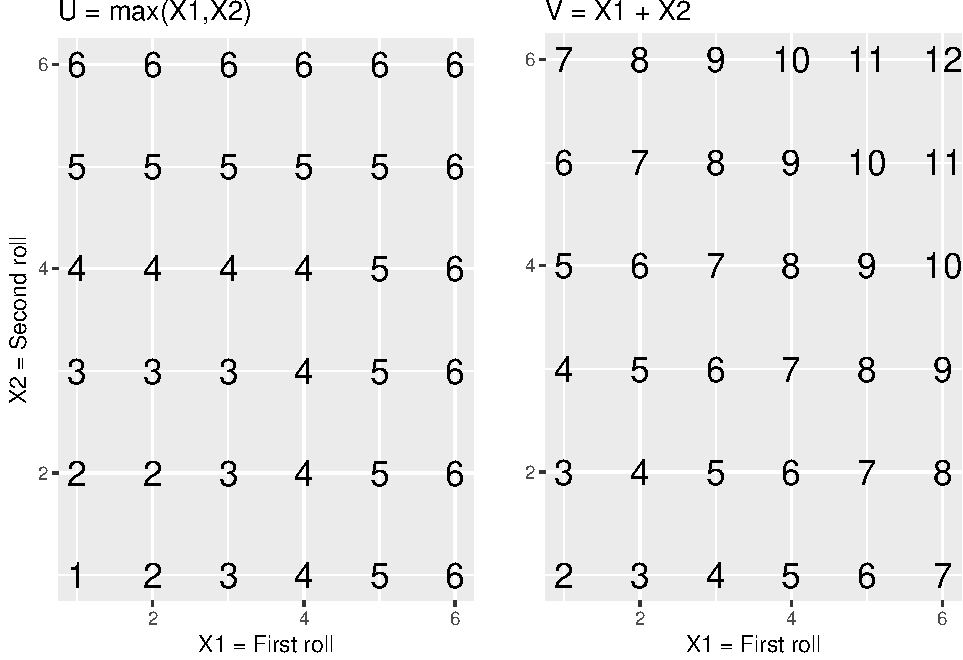
\includegraphics{_main_files/figure-latex/max-and-sum-two-dice-1.pdf}
\caption{\label{fig:max-and-sum-two-dice}\small Rolling two dice. The value of U
is the maximum of the two rolls, while the value of V is the sum of the
two rolls.}
\end{figure}





We may collapse the two matrices from Figure
\ref{fig:max-and-sum-two-dice} into one, big matrix of pairs of values
\((u,v)\). The result is shown in Table
\ref{fig:max-sum-two-dice-joint}.

\begin{figure}[htbp]
\centering
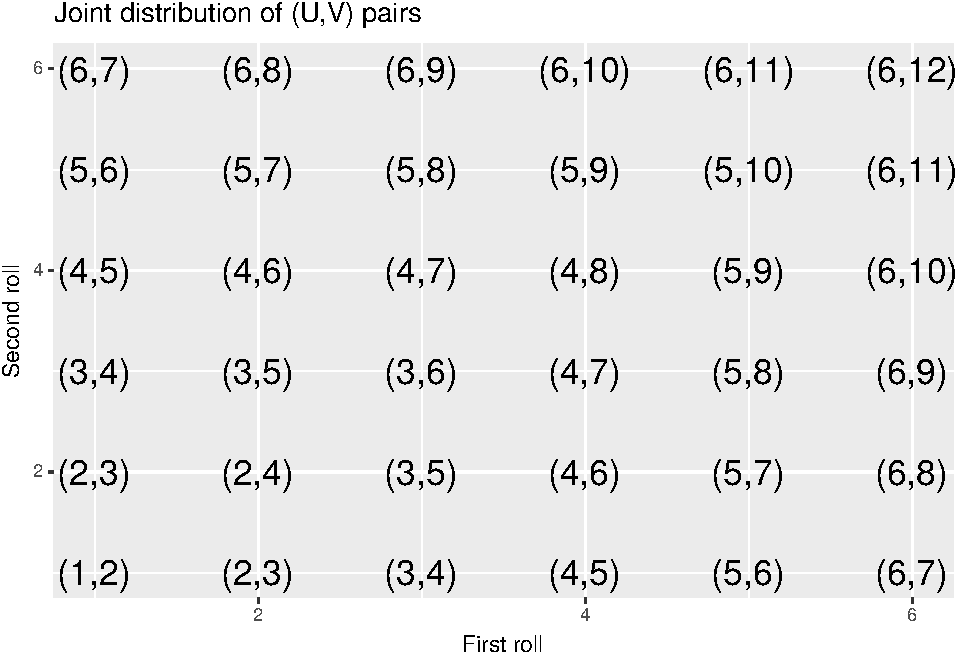
\includegraphics{_main_files/figure-latex/max-sum-two-dice-joint-1.pdf}
\caption{\label{fig:max-sum-two-dice-joint}(ref:cap-max-sum-two-dice)}
\end{figure}




Again, each of these pairs has probability \(1/36\) associated with it
and we are looking at the joint PDF of \((U,V)\) albeit in an unusual
form. Many of the pairs are repeated, but some of them are not:
\((1,2)\) appears only once, but \((2,3)\) appears twice. We can make
more sense out of this by writing a new table with \(U\) on one side and
\(V\) along the top. We will accumulate the probability just like we did
in Example \ref{ex:toss-two-dice-joint-pmf}. See Table
\ref{tab-max-sum-joint-pmf}.

(ref:tab-max-sum-joint-pm)

\begin{longtable}[]{@{}lllllllllllll@{}}
\caption{The joint PMF of \((U,V)\). The outcomes of \(U\) are along the
left and the outcomes of \(V\) are along the top. Empty entries in the
table have zero probability. The row totals (on the right) and column
totals (on the bottom) correspond to the marginal distribution of \(U\)
and \(V\), respectively.}\tabularnewline
\toprule
\begin{minipage}[b]{0.02\columnwidth}\raggedright\strut
\strut
\end{minipage} & \begin{minipage}[b]{0.05\columnwidth}\raggedright\strut
2\strut
\end{minipage} & \begin{minipage}[b]{0.05\columnwidth}\raggedright\strut
3\strut
\end{minipage} & \begin{minipage}[b]{0.05\columnwidth}\raggedright\strut
4\strut
\end{minipage} & \begin{minipage}[b]{0.05\columnwidth}\raggedright\strut
5\strut
\end{minipage} & \begin{minipage}[b]{0.05\columnwidth}\raggedright\strut
6\strut
\end{minipage} & \begin{minipage}[b]{0.05\columnwidth}\raggedright\strut
7\strut
\end{minipage} & \begin{minipage}[b]{0.05\columnwidth}\raggedright\strut
8\strut
\end{minipage} & \begin{minipage}[b]{0.05\columnwidth}\raggedright\strut
9\strut
\end{minipage} & \begin{minipage}[b]{0.05\columnwidth}\raggedright\strut
10\strut
\end{minipage} & \begin{minipage}[b]{0.05\columnwidth}\raggedright\strut
11\strut
\end{minipage} & \begin{minipage}[b]{0.05\columnwidth}\raggedright\strut
12\strut
\end{minipage} & \begin{minipage}[b]{0.05\columnwidth}\raggedright\strut
Total\strut
\end{minipage}\tabularnewline
\midrule
\endfirsthead
\toprule
\begin{minipage}[b]{0.02\columnwidth}\raggedright\strut
\strut
\end{minipage} & \begin{minipage}[b]{0.05\columnwidth}\raggedright\strut
2\strut
\end{minipage} & \begin{minipage}[b]{0.05\columnwidth}\raggedright\strut
3\strut
\end{minipage} & \begin{minipage}[b]{0.05\columnwidth}\raggedright\strut
4\strut
\end{minipage} & \begin{minipage}[b]{0.05\columnwidth}\raggedright\strut
5\strut
\end{minipage} & \begin{minipage}[b]{0.05\columnwidth}\raggedright\strut
6\strut
\end{minipage} & \begin{minipage}[b]{0.05\columnwidth}\raggedright\strut
7\strut
\end{minipage} & \begin{minipage}[b]{0.05\columnwidth}\raggedright\strut
8\strut
\end{minipage} & \begin{minipage}[b]{0.05\columnwidth}\raggedright\strut
9\strut
\end{minipage} & \begin{minipage}[b]{0.05\columnwidth}\raggedright\strut
10\strut
\end{minipage} & \begin{minipage}[b]{0.05\columnwidth}\raggedright\strut
11\strut
\end{minipage} & \begin{minipage}[b]{0.05\columnwidth}\raggedright\strut
12\strut
\end{minipage} & \begin{minipage}[b]{0.05\columnwidth}\raggedright\strut
Total\strut
\end{minipage}\tabularnewline
\midrule
\endhead
\begin{minipage}[t]{0.02\columnwidth}\raggedright\strut
1\strut
\end{minipage} & \begin{minipage}[t]{0.05\columnwidth}\raggedright\strut
\(\frac{1}{36}\)\strut
\end{minipage} & \begin{minipage}[t]{0.05\columnwidth}\raggedright\strut
\strut
\end{minipage} & \begin{minipage}[t]{0.05\columnwidth}\raggedright\strut
\strut
\end{minipage} & \begin{minipage}[t]{0.05\columnwidth}\raggedright\strut
\strut
\end{minipage} & \begin{minipage}[t]{0.05\columnwidth}\raggedright\strut
\strut
\end{minipage} & \begin{minipage}[t]{0.05\columnwidth}\raggedright\strut
\strut
\end{minipage} & \begin{minipage}[t]{0.05\columnwidth}\raggedright\strut
\strut
\end{minipage} & \begin{minipage}[t]{0.05\columnwidth}\raggedright\strut
\strut
\end{minipage} & \begin{minipage}[t]{0.05\columnwidth}\raggedright\strut
\strut
\end{minipage} & \begin{minipage}[t]{0.05\columnwidth}\raggedright\strut
\strut
\end{minipage} & \begin{minipage}[t]{0.05\columnwidth}\raggedright\strut
\strut
\end{minipage} & \begin{minipage}[t]{0.05\columnwidth}\raggedright\strut
\(\frac{1}{36}\)\strut
\end{minipage}\tabularnewline
\begin{minipage}[t]{0.02\columnwidth}\raggedright\strut
2\strut
\end{minipage} & \begin{minipage}[t]{0.05\columnwidth}\raggedright\strut
\strut
\end{minipage} & \begin{minipage}[t]{0.05\columnwidth}\raggedright\strut
\(\frac{2}{36}\)\strut
\end{minipage} & \begin{minipage}[t]{0.05\columnwidth}\raggedright\strut
\(\frac{1}{36}\)\strut
\end{minipage} & \begin{minipage}[t]{0.05\columnwidth}\raggedright\strut
\strut
\end{minipage} & \begin{minipage}[t]{0.05\columnwidth}\raggedright\strut
\strut
\end{minipage} & \begin{minipage}[t]{0.05\columnwidth}\raggedright\strut
\strut
\end{minipage} & \begin{minipage}[t]{0.05\columnwidth}\raggedright\strut
\strut
\end{minipage} & \begin{minipage}[t]{0.05\columnwidth}\raggedright\strut
\strut
\end{minipage} & \begin{minipage}[t]{0.05\columnwidth}\raggedright\strut
\strut
\end{minipage} & \begin{minipage}[t]{0.05\columnwidth}\raggedright\strut
\strut
\end{minipage} & \begin{minipage}[t]{0.05\columnwidth}\raggedright\strut
\strut
\end{minipage} & \begin{minipage}[t]{0.05\columnwidth}\raggedright\strut
\(\frac{3}{36}\)\strut
\end{minipage}\tabularnewline
\begin{minipage}[t]{0.02\columnwidth}\raggedright\strut
3\strut
\end{minipage} & \begin{minipage}[t]{0.05\columnwidth}\raggedright\strut
\strut
\end{minipage} & \begin{minipage}[t]{0.05\columnwidth}\raggedright\strut
\strut
\end{minipage} & \begin{minipage}[t]{0.05\columnwidth}\raggedright\strut
\(\frac{2}{36}\)\strut
\end{minipage} & \begin{minipage}[t]{0.05\columnwidth}\raggedright\strut
\(\frac{2}{36}\)\strut
\end{minipage} & \begin{minipage}[t]{0.05\columnwidth}\raggedright\strut
\(\frac{1}{36}\)\strut
\end{minipage} & \begin{minipage}[t]{0.05\columnwidth}\raggedright\strut
\strut
\end{minipage} & \begin{minipage}[t]{0.05\columnwidth}\raggedright\strut
\strut
\end{minipage} & \begin{minipage}[t]{0.05\columnwidth}\raggedright\strut
\strut
\end{minipage} & \begin{minipage}[t]{0.05\columnwidth}\raggedright\strut
\strut
\end{minipage} & \begin{minipage}[t]{0.05\columnwidth}\raggedright\strut
\strut
\end{minipage} & \begin{minipage}[t]{0.05\columnwidth}\raggedright\strut
\strut
\end{minipage} & \begin{minipage}[t]{0.05\columnwidth}\raggedright\strut
\(\frac{5}{36}\)\strut
\end{minipage}\tabularnewline
\begin{minipage}[t]{0.02\columnwidth}\raggedright\strut
4\strut
\end{minipage} & \begin{minipage}[t]{0.05\columnwidth}\raggedright\strut
\strut
\end{minipage} & \begin{minipage}[t]{0.05\columnwidth}\raggedright\strut
\strut
\end{minipage} & \begin{minipage}[t]{0.05\columnwidth}\raggedright\strut
\strut
\end{minipage} & \begin{minipage}[t]{0.05\columnwidth}\raggedright\strut
\(\frac{2}{36}\)\strut
\end{minipage} & \begin{minipage}[t]{0.05\columnwidth}\raggedright\strut
\(\frac{2}{36}\)\strut
\end{minipage} & \begin{minipage}[t]{0.05\columnwidth}\raggedright\strut
\(\frac{2}{36}\)\strut
\end{minipage} & \begin{minipage}[t]{0.05\columnwidth}\raggedright\strut
\(\frac{1}{36}\)\strut
\end{minipage} & \begin{minipage}[t]{0.05\columnwidth}\raggedright\strut
\strut
\end{minipage} & \begin{minipage}[t]{0.05\columnwidth}\raggedright\strut
\strut
\end{minipage} & \begin{minipage}[t]{0.05\columnwidth}\raggedright\strut
\strut
\end{minipage} & \begin{minipage}[t]{0.05\columnwidth}\raggedright\strut
\strut
\end{minipage} & \begin{minipage}[t]{0.05\columnwidth}\raggedright\strut
\(\frac{7}{36}\)\strut
\end{minipage}\tabularnewline
\begin{minipage}[t]{0.02\columnwidth}\raggedright\strut
5\strut
\end{minipage} & \begin{minipage}[t]{0.05\columnwidth}\raggedright\strut
\strut
\end{minipage} & \begin{minipage}[t]{0.05\columnwidth}\raggedright\strut
\strut
\end{minipage} & \begin{minipage}[t]{0.05\columnwidth}\raggedright\strut
\strut
\end{minipage} & \begin{minipage}[t]{0.05\columnwidth}\raggedright\strut
\strut
\end{minipage} & \begin{minipage}[t]{0.05\columnwidth}\raggedright\strut
\(\frac{2}{36}\)\strut
\end{minipage} & \begin{minipage}[t]{0.05\columnwidth}\raggedright\strut
\(\frac{2}{36}\)\strut
\end{minipage} & \begin{minipage}[t]{0.05\columnwidth}\raggedright\strut
\(\frac{2}{36}\)\strut
\end{minipage} & \begin{minipage}[t]{0.05\columnwidth}\raggedright\strut
\(\frac{2}{36}\)\strut
\end{minipage} & \begin{minipage}[t]{0.05\columnwidth}\raggedright\strut
\(\frac{1}{36}\)\strut
\end{minipage} & \begin{minipage}[t]{0.05\columnwidth}\raggedright\strut
\strut
\end{minipage} & \begin{minipage}[t]{0.05\columnwidth}\raggedright\strut
\strut
\end{minipage} & \begin{minipage}[t]{0.05\columnwidth}\raggedright\strut
\(\frac{9}{36}\)\strut
\end{minipage}\tabularnewline
\begin{minipage}[t]{0.02\columnwidth}\raggedright\strut
6\strut
\end{minipage} & \begin{minipage}[t]{0.05\columnwidth}\raggedright\strut
\strut
\end{minipage} & \begin{minipage}[t]{0.05\columnwidth}\raggedright\strut
\strut
\end{minipage} & \begin{minipage}[t]{0.05\columnwidth}\raggedright\strut
\strut
\end{minipage} & \begin{minipage}[t]{0.05\columnwidth}\raggedright\strut
\strut
\end{minipage} & \begin{minipage}[t]{0.05\columnwidth}\raggedright\strut
\strut
\end{minipage} & \begin{minipage}[t]{0.05\columnwidth}\raggedright\strut
\(\frac{2}{36}\)\strut
\end{minipage} & \begin{minipage}[t]{0.05\columnwidth}\raggedright\strut
\(\frac{2}{36}\)\strut
\end{minipage} & \begin{minipage}[t]{0.05\columnwidth}\raggedright\strut
\(\frac{2}{36}\)\strut
\end{minipage} & \begin{minipage}[t]{0.05\columnwidth}\raggedright\strut
\(\frac{2}{36}\)\strut
\end{minipage} & \begin{minipage}[t]{0.05\columnwidth}\raggedright\strut
\(\frac{2}{36}\)\strut
\end{minipage} & \begin{minipage}[t]{0.05\columnwidth}\raggedright\strut
\(\frac{1}{36}\)\strut
\end{minipage} & \begin{minipage}[t]{0.05\columnwidth}\raggedright\strut
\(\frac{11}{36}\)\strut
\end{minipage}\tabularnewline
\begin{minipage}[t]{0.02\columnwidth}\raggedright\strut
-------+------------------+------------------+------------------+------------------+------------------+------------------+------------------+------------------+------------------+------------------+------------------+------------------\strut
\end{minipage} & \begin{minipage}[t]{0.05\columnwidth}\raggedright\strut
\strut
\end{minipage}\tabularnewline
\begin{minipage}[t]{0.02\columnwidth}\raggedright\strut
Total\strut
\end{minipage} & \begin{minipage}[t]{0.05\columnwidth}\raggedright\strut
\(\frac{1}{36}\)\strut
\end{minipage} & \begin{minipage}[t]{0.05\columnwidth}\raggedright\strut
\(\frac{2}{36}\)\strut
\end{minipage} & \begin{minipage}[t]{0.05\columnwidth}\raggedright\strut
\(\frac{3}{36}\)\strut
\end{minipage} & \begin{minipage}[t]{0.05\columnwidth}\raggedright\strut
\(\frac{4}{36}\)\strut
\end{minipage} & \begin{minipage}[t]{0.05\columnwidth}\raggedright\strut
\(\frac{5}{36}\)\strut
\end{minipage} & \begin{minipage}[t]{0.05\columnwidth}\raggedright\strut
\(\frac{6}{36}\)\strut
\end{minipage} & \begin{minipage}[t]{0.05\columnwidth}\raggedright\strut
\(\frac{5}{36}\)\strut
\end{minipage} & \begin{minipage}[t]{0.05\columnwidth}\raggedright\strut
\(\frac{4}{36}\)\strut
\end{minipage} & \begin{minipage}[t]{0.05\columnwidth}\raggedright\strut
\(\frac{3}{36}\)\strut
\end{minipage} & \begin{minipage}[t]{0.05\columnwidth}\raggedright\strut
\(\frac{2}{36}\)\strut
\end{minipage} & \begin{minipage}[t]{0.05\columnwidth}\raggedright\strut
\(\frac{1}{36}\)\strut
\end{minipage} & \begin{minipage}[t]{0.05\columnwidth}\raggedright\strut
1\strut
\end{minipage}\tabularnewline
\bottomrule
\end{longtable}

The joint support of \((U,V)\) is concentrated along the main diagonal;
note that the nonzero entries do not form a rectangle. Also notice that
if we form row and column totals we are doing exactly the same thing as
Equation \eqref{eq-marginal-pmf}, so that the marginal distribution of
\(U\) is the list of totals in the right ``margin'' of the Table
\ref{tab-max-sum-joint-pmf}, and the marginal distribution of \(V\) is
the list of totals in the bottom ``margin''.

Continuing the reasoning for the discrete case, given two continuous
random variables \(X\) and \(Y\) there similarly exists\footnote{We are
  taking great leaps over the mathematical details. In particular, we
  have yet to show that \(s^{2}\) has a chi-square distribution and we
  have not even come close to showing that \(b_{i}\) and \(s_{b_{i}}\)
  are independent. But these are entirely outside the scope of the
  present book and the reader may rest assured that the proofs await in
  later classes. See C.R. Rao for more.} a function \(f_{X,Y}(x,y)\)
associated with \(X\) and \(Y\) called the \emph{joint probability
density function} of \(X\) and \(Y\). Every joint PDF satisfies

\begin{equation}
f_{X,Y}(x,y)\geq0\mbox{ for all }(x,y)\in S_{X,Y},
\end{equation}

and

\begin{equation}
\iintop_{S_{X,Y}}f_{X,Y}(x,y)\,\mathrm{d} x\,\mathrm{d} y=1.
\end{equation}

In the continuous case there is not such a simple interpretation for the
joint PDF; however, we do have one for the joint CDF, namely, \[
F_{X,Y}(x,y)=\mathbb{P}(X\leq x,\, Y\leq
y)=\int_{-\infty}^{x}\int_{-\infty}^{y}f_{X,Y}(u,v)\,\mathrm{d}
v\,\mathrm{d} u, \] for \((x,y)\in\mathbb{R}^{2}\). If \(X\) and \(Y\)
have the joint PDF \(f_{X,Y}\), then the marginal density of \(X\) may
be recovered by

\begin{equation}
f_{X}(x)=\int_{S_{Y}}f_{X,Y}(x,y)\,\mathrm{d} y,\quad x \in S_{X}
\end{equation}

and the marginal PDF of \(Y\) may be found with

\begin{equation}
f_{Y}(y)=\int_{S_{X}}f_{X,Y}(x,y)\,\mathrm{d} x, \quad y \in S_{Y}.
\end{equation}

\bigskip

\BeginKnitrBlock{example}
\protect\hypertarget{ex:joint-pdf}{}{\label{ex:joint-pdf}}Let the joint PDF
of \((X,Y)\) be given by \[
f_{X,Y}(x,y)=\frac{6}{5}\left(x+y^{2}\right),\quad 0 < x < 1,\ 0 < y
< 1.  \] The marginal PDF of \(X\) is

\begin{eqnarray*}
f_{X}(x) & = & \int_{0}^{1}\frac{6}{5}\left(x+y^{2}\right)\,\mathrm{d} y,\\
 & = & \left.\frac{6}{5}\left(xy+\frac{y^{3}}{3}\right)\right|_{y=0}^{1},\\
 & = & \frac{6}{5}\left(x+\frac{1}{3}\right),
\end{eqnarray*}

for \(0 < x < 1\), and the marginal PDF of \(Y\) is

\begin{eqnarray*}
f_{Y}(y) & = & \int_{0}^{1}\frac{6}{5}\left(x+y^{2}\right)\,\mathrm{d} x,\\
 & = & \left.\frac{6}{5}\left(\frac{x^{2}}{2}+xy^{2}\right)\right|_{x=0}^{1},\\
 & = & \frac{6}{5}\left(\frac{1}{2}+y^{2}\right),
\end{eqnarray*}

for \(0 < y < 1\). In this example the joint support set was a rectangle
\([0,1]\times[0,1]\), but it turns out that \(X\) and \(Y\) are not
independent. See Section \ref{sec-independent-random-variables}.
\EndKnitrBlock{example}

\subsection{How to do it with R}\label{how-to-do-it-with-r-20}

We will show how to do Example \ref{ex:max-sum-two-dice} using R; it is
much simpler to do it with R than without. First we set up the sample
space with the \texttt{rolldie} function. Next, we add random variables
\(U\) and \(V\) with the \texttt{addrv} function. We take a look at the
very top of the data frame (probability space) to make sure that
everything is operating according to plan.

\begin{Shaded}
\begin{Highlighting}[]
\NormalTok{S <-}\StringTok{ }\KeywordTok{rolldie}\NormalTok{(}\DecValTok{2}\NormalTok{, }\DataTypeTok{makespace =} \OtherTok{TRUE}\NormalTok{)}
\NormalTok{S <-}\StringTok{ }\KeywordTok{addrv}\NormalTok{(S, }\DataTypeTok{FUN =} \NormalTok{max, }\DataTypeTok{invars =} \KeywordTok{c}\NormalTok{(}\StringTok{"X1"}\NormalTok{,}\StringTok{"X2"}\NormalTok{), }\DataTypeTok{name =} \StringTok{"U"}\NormalTok{)}
\NormalTok{S <-}\StringTok{ }\KeywordTok{addrv}\NormalTok{(S, }\DataTypeTok{FUN =} \NormalTok{sum, }\DataTypeTok{invars =} \KeywordTok{c}\NormalTok{(}\StringTok{"X1"}\NormalTok{,}\StringTok{"X2"}\NormalTok{), }\DataTypeTok{name =} \StringTok{"V"}\NormalTok{)}
\KeywordTok{head}\NormalTok{(S)}
\end{Highlighting}
\end{Shaded}

\begin{verbatim}
  X1 X2 U V      probs
1  1  1 1 2 0.02777778
2  2  1 2 3 0.02777778
3  3  1 3 4 0.02777778
4  4  1 4 5 0.02777778
5  5  1 5 6 0.02777778
6  6  1 6 7 0.02777778
\end{verbatim}

Yes, the \(U\) and \(V\) columns have been added to the data frame and
have been computed correctly. This result would be fine as it is, but
the data frame has too many rows: there are repeated pairs \((u,v)\)
which show up as repeated rows in the data frame. The goal is to
aggregate the rows of \(S\) such that the result has exactly one row for
each unique pair \((u,v)\) with positive probability. This sort of thing
is exactly the task for which the \texttt{marginal} function was
designed. We may take a look at the joint distribution of \(U\) and
\(V\) (we only show the first few rows of the data frame, but the
complete one has 11 rows).

\begin{Shaded}
\begin{Highlighting}[]
\NormalTok{UV <-}\StringTok{ }\KeywordTok{marginal}\NormalTok{(S, }\DataTypeTok{vars =} \KeywordTok{c}\NormalTok{(}\StringTok{"U"}\NormalTok{, }\StringTok{"V"}\NormalTok{))}
\KeywordTok{head}\NormalTok{(UV)}
\end{Highlighting}
\end{Shaded}

\begin{verbatim}
  U V      probs
1 1 2 0.02777778
2 2 3 0.05555556
3 2 4 0.02777778
4 3 4 0.05555556
5 3 5 0.05555556
6 4 5 0.05555556
\end{verbatim}

The data frame is difficult to understand. It would be better to have a
tabular display like Table \ref{tab-max-sum-joint-pmf}. We can do that
with the \texttt{xtabs} function.

\begin{Shaded}
\begin{Highlighting}[]
\KeywordTok{xtabs}\NormalTok{(}\KeywordTok{round}\NormalTok{(probs,}\DecValTok{3}\NormalTok{) ~}\StringTok{ }\NormalTok{U +}\StringTok{ }\NormalTok{V, }\DataTypeTok{data =} \NormalTok{UV)}
\end{Highlighting}
\end{Shaded}

\begin{verbatim}
   V
U       2     3     4     5     6     7     8     9    10
  1 0.028 0.000 0.000 0.000 0.000 0.000 0.000 0.000 0.000
  2 0.000 0.056 0.028 0.000 0.000 0.000 0.000 0.000 0.000
  3 0.000 0.000 0.056 0.056 0.028 0.000 0.000 0.000 0.000
  4 0.000 0.000 0.000 0.056 0.056 0.056 0.028 0.000 0.000
  5 0.000 0.000 0.000 0.000 0.056 0.056 0.056 0.056 0.028
  6 0.000 0.000 0.000 0.000 0.000 0.056 0.056 0.056 0.056
   V
U      11    12
  1 0.000 0.000
  2 0.000 0.000
  3 0.000 0.000
  4 0.000 0.000
  5 0.000 0.000
  6 0.056 0.028
\end{verbatim}

Compare these values to the ones shown in Table
\ref{tab-max-sum-joint-pmf}. We can repeat the process with
\texttt{marginal} to get the univariate marginal distributions of \(U\)
and \(V\) separately.

\begin{Shaded}
\begin{Highlighting}[]
\KeywordTok{marginal}\NormalTok{(UV, }\DataTypeTok{vars =} \StringTok{"U"}\NormalTok{)}
\end{Highlighting}
\end{Shaded}

\begin{verbatim}
  U      probs
1 1 0.02777778
2 2 0.08333333
3 3 0.13888889
4 4 0.19444444
5 5 0.25000000
6 6 0.30555556
\end{verbatim}

\begin{Shaded}
\begin{Highlighting}[]
\KeywordTok{head}\NormalTok{(}\KeywordTok{marginal}\NormalTok{(UV, }\DataTypeTok{vars =} \StringTok{"V"}\NormalTok{))}
\end{Highlighting}
\end{Shaded}

\begin{verbatim}
  V      probs
1 2 0.02777778
2 3 0.05555556
3 4 0.08333333
4 5 0.11111111
5 6 0.13888889
6 7 0.16666667
\end{verbatim}

Another way to do the same thing is with the \texttt{rowSums} and
\texttt{colSums} of the \texttt{xtabs} object. Compare

\begin{Shaded}
\begin{Highlighting}[]
\NormalTok{temp <-}\StringTok{ }\KeywordTok{xtabs}\NormalTok{(probs ~}\StringTok{ }\NormalTok{U +}\StringTok{ }\NormalTok{V, }\DataTypeTok{data =} \NormalTok{UV)}
\KeywordTok{rowSums}\NormalTok{(temp)}
\end{Highlighting}
\end{Shaded}

\begin{verbatim}
         1          2          3          4          5 
0.02777778 0.08333333 0.13888889 0.19444444 0.25000000 
         6 
0.30555556 
\end{verbatim}

\begin{Shaded}
\begin{Highlighting}[]
\KeywordTok{colSums}\NormalTok{(temp)}
\end{Highlighting}
\end{Shaded}

\begin{verbatim}
         2          3          4          5          6 
0.02777778 0.05555556 0.08333333 0.11111111 0.13888889 
         7          8          9         10         11 
0.16666667 0.13888889 0.11111111 0.08333333 0.05555556 
        12 
0.02777778 
\end{verbatim}

You should check that the answers that we have obtained exactly match
the same (somewhat laborious) calculations that we completed in Example
\ref{ex:max-sum-two-dice}.

\section{Joint and Marginal
Expectation}\label{sec-joint-and-marginal-expectation}

Given a function \(g\) with arguments \((x,y)\) we would like to know
the long-run average behavior of \(g(X,Y)\) and how to mathematically
calculate it. Expectation in this context is computed in the pedestrian
way. We simply integrate (sum) with respect to the joint probability
density (mass) function.

\begin{equation}
\mathbb{E}\, g(X,Y)=\iintop_{S_{X,Y}}g(x,y)\, f_{X,Y}(x,y)\,\mathrm{d} x\,\mathrm{d} y,
\end{equation}

or in the discrete case,

\begin{equation}
\mathbb{E}\, g(X,Y)=\mathop{\sum\sum}\limits _{(x,y)\in S_{X,Y}}g(x,y)\, f_{X,Y}(x,y).
\end{equation}

\subsection{Covariance and
Correlation}\label{covariance-and-correlation}

There are two very special cases of joint expectation: the
\emph{covariance} and the \emph{correlation}. These are measures which
help us quantify the dependence between \(X\) and \(Y\).

\bigskip

\BeginKnitrBlock{definition}
\protect\hypertarget{def:unnamed-chunk-201}{}{\label{def:unnamed-chunk-201}}The
\emph{covariance} of \(X\) and \(Y\) is

\begin{equation}
\mbox{Cov}(X,Y)=\mathbb{E}(X-\mathbb{E} X)(Y-\mathbb{E} Y).
\end{equation}
\EndKnitrBlock{definition}

By the way, there is a shortcut formula for covariance which is almost
as handy as the shortcut for the variance:

\begin{equation}
\mbox{Cov}(X,Y)=\mathbb{E}(XY)-(\mathbb{E} X)(\mathbb{E} Y).
\end{equation}

The proof is left to Exercise \ref{xca-prove-cov-shortcut}.

The Pearson product moment correlation between \(X\) and \(Y\) is the
covariance between \(X\) and \(Y\) rescaled to fall in the interval
\([-1,1]\). It is formally defined by

\begin{equation}
\mbox{Corr}(X,Y)=\frac{\mbox{Cov}(X,Y)}{\sigma_{X}\sigma_{Y}}.
\end{equation}

The correlation is usually denoted by \(\rho_{X,Y}\) or simply \(\rho\)
if the random variables are clear from context. There are some important
facts about the correlation coefficient: 1. The range of correlation is
\(-1\leq\rho_{X,Y}\leq1\). 1. Equality holds above (\(\rho_{X,Y}=\pm1\))
if and only if \(Y\) is a linear function of \(X\) with probability one.

\bigskip

\BeginKnitrBlock{example}
\protect\hypertarget{ex:max-sum-dice-covariance}{}{\label{ex:max-sum-dice-covariance}}We
will compute the covariance for the discrete distribution in Example
\ref{ex:max-sum-two-dice}. The expected value of \(U\) is
\[ \mathbb{E} U=\sum_{u=1}^{6}u\,
f_{U}(u)=\sum_{u=1}^{6}u\,\frac{2u-1}{36}=1\left(\frac{1}{36}\right)+2\left(\frac{3}{36}\right)+\cdots+6\left(\frac{11}{36}\right)=\frac{161}{36},
\] and the expected value of \(V\) is \[ \mathbb{E}
V=\sum_{v=2}^{12}v\,\frac{6-|7-v|}{36}=2\left(\frac{1}{36}\right)+3\left(\frac{2}{36}\right)+\cdots+12\left(\frac{1}{36}\right)=7,
\] and the expected value of \(UV\) is \[ \mathbb{E}
UV=\sum_{u=1}^{6}\sum_{v=2}^{12}uv\,
f_{U,V}(u,v)=1\cdot2\left(\frac{1}{36}\right)+2\cdot3\left(\frac{2}{36}\right)+\cdots+6\cdot12\left(\frac{1}{36}\right)=\frac{308}{9}.
\] Therefore the covariance of \((U,V)\) is \[
\mbox{Cov}(U,V)=\mathbb{E} UV-\left(\mathbb{E}
U\right)\left(\mathbb{E}
V\right)=\frac{308}{9}-\frac{161}{36}\cdot7=\frac{35}{12}.
\] All we need now are the standard deviations of \(U\) and \(V\) to
calculate the correlation coefficient (omitted).
\EndKnitrBlock{example}

We will do a continuous example so that you can see how it works.

\bigskip

\BeginKnitrBlock{example}
\protect\hypertarget{ex:unnamed-chunk-202}{}{\label{ex:unnamed-chunk-202}}Let
us find the covariance of the variables \((X,Y)\) from Example
\ref{ex:joint-pdf}. The expected value of \(X\) is \[ \mathbb{E}
X=\int_{0}^{1}x\cdot\frac{6}{5}\left(x+\frac{1}{3}\right)\mathrm{d}
x=\left.\frac{2}{5}x^{3}+\frac{1}{5}x^{2}\right|_{x=0}^{1}=\frac{3}{5},
\] and the expected value of \(Y\) is \[ \mathbb{E}
Y=\int_{0}^{1}y\cdot\frac{6}{5}\left(\frac{1}{2}+y^{2}\right)\mathrm{d}
x=\left.\frac{3}{10}y^{2}+\frac{3}{20}y^{4}\right|_{y=0}^{1}=\frac{9}{20}.
\] Finally, the expected value of \(XY\) is

\begin{eqnarray*}
\mathbb{E} XY & = & \int_{0}^{1}\int_{0}^{1}xy\,\frac{6}{5}\left(x+y^{2}\right)\mathrm{d} x\,\mathrm{d} y,\\
 & = & \int_{0}^{1}\left.\left(\frac{2}{5}x^{3}y+\frac{3}{5}x^{2}y^{3}\right)\right|_{x=0}^{1}\mathrm{d} y,\\
 & = & \int_{0}^{1}\left(\frac{2}{5}y+\frac{3}{5}y^{3}\right)\mathrm{d} y,\\
 & = & \frac{1}{5}+\frac{3}{20},
\end{eqnarray*}

which is 7/20. Therefore the covariance of \((X,Y)\) is \[
\mbox{Cov}(X,Y)=\frac{7}{20}-\left(\frac{3}{5}\right)\left(\frac{9}{20}\right)=\frac{2}{25}.
\]
\EndKnitrBlock{example}

\subsubsection{How to do it with R}\label{how-to-do-it-with-r-21}

There are not any specific functions in the \texttt{prob} package
\autocite{prob} designed for multivariate expectation. This is not a
problem, though, because it is easy enough to do expectation the long
way -- with column operations. We just need to keep the definition in
mind. For instance, we may compute the covariance of \((U,V)\) from
Example \ref{ex:max-sum-dice-covariance}.

\begin{Shaded}
\begin{Highlighting}[]
\NormalTok{Eu <-}\StringTok{ }\KeywordTok{sum}\NormalTok{(S$U*S$probs)}
\NormalTok{Ev <-}\StringTok{ }\KeywordTok{sum}\NormalTok{(S$V*S$probs)}
\NormalTok{Euv <-}\StringTok{ }\KeywordTok{sum}\NormalTok{(S$U*S$V*S$probs)}
\NormalTok{Euv -}\StringTok{ }\NormalTok{Eu *}\StringTok{ }\NormalTok{Ev}
\end{Highlighting}
\end{Shaded}

\begin{verbatim}
[1] 2.916667
\end{verbatim}

Compare this answer to what we got in Example
\ref{ex:max-sum-dice-covariance}.

To do the continuous case we could use the computer algebra utilities of
\texttt{Yacas} and the associated R package \texttt{Ryacas}
\autocite{Ryacas}. See Section \ref{sub-bivariate-transf-r} for another
example where the \texttt{Ryacas} package appears.

\section{Conditional Distributions}\label{sec-conditional-distributions}

If \(x\in S_{X}\) is such that \(f_{X}(x)>0\), then we define the
\emph{conditional density} of \(Y|\, X=x\), denoted \(f_{Y|x}\), by

\begin{equation}
f_{Y|x}(y|x)=\frac{f_{X,Y}(x,y)}{f_{X}(x)},\quad y\in S_{Y}.
\end{equation}

We define \(f_{X|y}\) in a similar fashion.

BLANK

\bigskip

\BeginKnitrBlock{example}
\protect\hypertarget{ex:unnamed-chunk-204}{}{\label{ex:unnamed-chunk-204}}Let
the joint PMF of \(X\) and \(Y\) be given by \[
f_{X,Y}(x,y) =
\]
\EndKnitrBlock{example}

\subsection{Bayesian Connection}\label{bayesian-connection}

Conditional distributions play a fundamental role in Bayesian
probability and statistics. There is a parameter \(\theta\) which is of
primary interest, and about which we would like to learn. But rather
than observing \(\theta\) directly, we instead observe a random variable
\(X\) whose probability distribution depends on \(\theta\). Using the
information we provided by \(X,\) we would like to update the
information that we have about \(\theta\).

Our initial beliefs about \(\theta\) are represented by a probability
distribution, called the \emph{prior distribution}, denoted by \(\pi\).
The PDF \(f_{X|\theta}\) is called the \emph{likelihood function}, also
called the \emph{likelihood of} \(X\) \emph{conditional on} \(\theta\).
Given an observation \(X=x\), we would like to update our beliefs
\(\pi\) to a new distribution, called the \emph{posterior distribution
of} \(\theta\) \emph{given the observation} \(X=x\), denoted
\(\pi_{\theta|x}\). It may seem a mystery how to obtain
\(\pi_{\theta|x}\) based only on the information provided by \(\pi\) and
\(f_{X|\theta}\), but it should not be. We have already studied this in
Section \ref{sec-bayes-rule} where it was called Bayes' Rule:

\begin{equation} 
\pi(\theta|x)=\frac{\pi(\theta)\, f(x|\theta)}{\int\pi(u)\, f(x|u)\mathrm{d} u}.
\end{equation}

Compare the above expression to Equation \eqref{eq-bayes-rule}.

\bigskip

\BeginKnitrBlock{example}
\protect\hypertarget{ex:unnamed-chunk-205}{}{\label{ex:unnamed-chunk-205}}Suppose
the parameter \(\theta\) is the \(\mathbb{P}(\mbox{Heads})\) for a
biased coin. It could be any value from 0 to 1. Perhaps we have some
prior information about this coin, for example, maybe we have seen this
coin before and we have reason to believe that it shows Heads less than
half of the time. Suppose that we represent our beliefs about \(\theta\)
with a \(\mathsf{beta}(\mathtt{shape1}=1,\,\mathtt{shape2}=3)\) prior
distribution, that is, we assume \[
\theta\sim\pi(\theta)=3(1-\theta)^{2},\quad 0 < \theta < 1.  \] To learn
more about \(\theta\), we will do what is natural: flip the coin. We
will observe a random variable \(X\) which takes the value \(1\) if the
coin shows Heads, and 0 if the coin shows Tails. Under these
circumstances, \(X\) will have a Bernoulli distribution, and in
particular,
\(X|\theta\sim\mathsf{binom}(\mathtt{size}=1,\,\mathtt{prob}=\theta)\):
\[ f_{X|\theta}(x|\theta)=\theta^{x}(1-\theta)^{1-x},\quad x=0,1.  \]
Based on the observation \(X=x\), we will update the prior distribution
to the posterior distribution, and we will do so with Bayes' Rule: it
says

\begin{eqnarray*}
\pi(\theta|x) & \propto & f(x|\theta) \, \pi(\theta),\\
 & = & \theta^{x}(1-\theta)^{1-x}\cdot3(1-\theta)^{2},\\
 & = & 3\,\theta^{x}(1-\theta)^{3-x},\quad 0 < \theta < 1,
\end{eqnarray*}

where the constant of proportionality is given by \[ \int3\,
u^{x}(1-u)^{3-x}\mathrm{d} u=\int3\,
u^{(1+x)-1}(1-u)^{(4-x)-1}\mathrm{d}
u=3\,\frac{\Gamma(1+x)\Gamma(4-x)}{\Gamma[(1+x)+(4-x)]}, \] the integral
being calculated by inspection of the formula for a
\(\mathsf{beta}(\mathtt{shape1}=1+x,\,\mathtt{shape2}=4-x)\)
distribution. That is to say, our posterior distribution is precisely \[
\theta|x\sim\mathsf{beta}(\mathtt{shape1}=1+x,\,\mathtt{shape2}=4-x).
\] The Bayesian statistician uses the posterior distribution for all
matters concerning inference about \(\theta\).
\EndKnitrBlock{example}

\bigskip

\begin{remark}
We usually do not restrict ourselves to the observation of only one
\(X\) conditional on \(\theta\). In fact, it is common to observe an
entire sample \(X_{1}\), \(X_{2}\),\ldots{},\(X_{n}\) conditional on
\(\theta\) (which itself is often multidimensional). Do not be
frightened, however, because the intuition is the same. There is a prior
distribution \(\pi(\theta)\), a likelihood
\(f(x_{1},x_{2},\ldots,x_{n}|\theta)\), and a posterior distribution
\(\pi(\theta|x_{1},x_{2},\ldots,x_{n})\). Bayes' Rule states that the
relationship between the three is \[
\pi(\theta|x_{1},x_{2},\ldots,x_{n})\propto\pi(\theta)\,
f(x_{1},x_{2},\ldots,x_{n}|\theta), \] where the constant of
proportionality is
\(\int\pi(u)\, f(x_{1},x_{2},\ldots,x_{n}|u)\,\mathrm{d} u\).
\end{remark}

Any good textbook on Bayesian Statistics will explain these notions in
detail; to the interested reader I recommend Gelman
\autocite{Gelman2004} or Lee \autocite{Lee1997}.

\section{Independent Random
Variables}\label{sec-independent-random-variables}

\subsection{Independent Random
Variables}\label{sub-independent-random-variables}

We recall from Chapter \ref{cha-probability} that the events \(A\) and
\(B\) are said to be independent when

\begin{equation}
\mathbb{P}(A\cap B)=\mathbb{P}(A)\mathbb{P}(B).
\end{equation}

If it happens that

\begin{equation}
\mathbb{P}(X=x,Y=y)=\mathbb{P}(X=x)\mathbb{P}(Y=y),\quad \mbox{for every }x\in S_{X},\ y\in S_{Y},
\end{equation}

then we say that \(X\) and \(Y\) are \emph{independent random
variables}. Otherwise, we say that \(X\) and \(Y\) are \emph{dependent}.
Using the PMF notation from above, we see that independent discrete
random variables satisfy

\begin{equation}
f_{X,Y}(x,y)=f_{X}(x)f_{Y}(y)\quad \mbox{for every }x\in S_{X},\ y\in S_{Y}.
\end{equation}

Continuing the reasoning, given two continuous random variables \(X\)
and \(Y\) with joint PDF \(f_{X,Y}\) and respective marginal PDFs
\(f_{X}\) and \(f_{Y}\) that are supported on the sets \(S_{X}\) and
\(S_{Y}\), if it happens that

\begin{equation}
f_{X,Y}(x,y)=f_{X}(x)f_{Y}(y)\quad \mbox{for every }x\in S_{X},\ y\in S_{Y},
\end{equation}

then we say that \(X\) and \(Y\) are independent.

\bigskip

\BeginKnitrBlock{example}
\protect\hypertarget{ex:unnamed-chunk-207}{}{\label{ex:unnamed-chunk-207}}In
Example \ref{ex:toss-two-dice-joint-pmf} we considered the random
experiment of rolling a fair die twice. There we found the joint PMF to
be \[
f_{X,Y}(x,y)=\frac{1}{36},\quad x=1,\ldots,6,\ y=1,\ldots,6,
\] and we found the marginal PMFs \(f_{X}(x)=1/6\), \(x=1,2,\ldots,6\),
and \(f_{Y}(y)=1/6\), \(y=1,2,\ldots,6\). Therefore in this experiment
\(X\) and \(Y\) are independent since for every \(x\) and \(y\) in the
joint support the joint PMF satisfies \[
f_{X,Y}(x,y)=\frac{1}{36}=\left(\frac{1}{6}\right)\left(\frac{1}{6}\right)=f_{X}(x)\,
f_{Y}(y). 
\]
\EndKnitrBlock{example}

\bigskip

\BeginKnitrBlock{example}
\protect\hypertarget{ex:unnamed-chunk-208}{}{\label{ex:unnamed-chunk-208}}In
Example \ref{ex:max-sum-two-dice} we considered the same experiment but
different random variables \(U\) and \(V\). We can prove that \(U\) and
\(V\) are not independent if we can find a single pair \((u,v)\) where
the independence equality does not hold. There are many such pairs. One
of them is \((6,12)\): \[
f_{U,V}(6,12)=\frac{1}{36}\neq\left(\frac{11}{36}\right)\left(\frac{1}{36}\right)=f_{U}(6)\,
f_{V}(12).  
\]
\EndKnitrBlock{example}

Independent random variables are very useful to the mathematician. They
have many, many, tractable properties. We mention some of the more
important ones.

\bigskip

\BeginKnitrBlock{proposition}
\protect\hypertarget{prp:indep-implies-prodexpect}{}{\label{prp:indep-implies-prodexpect}}If
\(X\) and \(Y\) are independent, then for any functions \(u\) and \(v\),

\begin{equation}
\mathbb{E}\left(u(X)v(Y)\right)=\left(\mathbb{E} u(X)\right)\left(\mathbb{E} v(Y)\right).
\end{equation}
\EndKnitrBlock{proposition}

\bigskip

\BeginKnitrBlock{proof}
\iffalse {Proof. } \fi This is straightforward from the definition.

\begin{eqnarray*}
\mathbb{E}\left(u(X)v(Y)\right) & = & \iint\, u(x)v(y)\, f_{X,Y}(x,y)\,\mathrm{d} x\mathrm{d} y\\
 & = & \iint\, u(x)v(y)\, f_{X}(x)\, f_{Y}(y)\,\mathrm{d} x\mathrm{d} y\\
 & = & \int u(x)\, f_{X}(x)\,\mathrm{d} x\ \int v(y)\, f_{Y}(y)\,\mathrm{d} y
\end{eqnarray*}

and this last quantity is exactly
\(\left(\mathbb{E} u(X)\right)\left(\mathbb{E} v(Y)\right)\).
\EndKnitrBlock{proof}

Now that we have Proposition \ref{pro:indep-implies-prodexpect} we
mention a corollary that will help us later to quickly identify those
random variables which are \emph{not} independent.

\bigskip

\BeginKnitrBlock{corollary}
\protect\hypertarget{cor:cor-indep-implies-uncorr}{}{\label{cor:cor-indep-implies-uncorr}}If
\(X\) and \(Y\) are independent, then \(\mbox{Cov}(X,Y)=0\), and
consequently, \(\mbox{Corr}(X,Y)=0\).
\EndKnitrBlock{corollary}

\bigskip

\BeginKnitrBlock{proof}
\iffalse {Proof. } \fi When \(X\) and \(Y\) are independent then
\(\mathbb{E} XY=\mathbb{E} X\,\mathbb{E} Y\). And when the covariance is
zero the numerator of the correlation is 0.
\EndKnitrBlock{proof}

\bigskip

\begin{remark}
Unfortunately, the converse of Corollary \ref{cor:indep-implies-uncorr}
is not true. That is, there are many random variables which are
dependent yet their covariance and correlation is zero.
\end{remark}

For more details, see Casella and Berger \autocite{Casella2002}.
Proposition \ref{pro:indep-implies-prodexpect} is useful to us and we
will receive mileage out of it, but there is another fact which will
play an even more important role. Unfortunately, the proof is beyond the
techniques presented here. The inquisitive reader should consult Casella
and Berger \autocite{Casella2002}, Resnick \autocite{Resnick1999},
\emph{etc}.

\bigskip

\begin{fact}
If \(X\) and \(Y\) are independent, then \(u(X)\) and \(v(Y)\) are
independent for any functions \(u\) and \(v\).
\end{fact}

\subsection{Combining Independent Random
Variables}\label{sub-combining-independent-random}

Another important corollary of Proposition
\ref{pro:indep-implies-prodexpect} will allow us to find the
distribution of sums of random variables.

\bigskip

\BeginKnitrBlock{corollary}
\protect\hypertarget{cor:unnamed-chunk-211}{}{\label{cor:unnamed-chunk-211}}If
\(X\) and \(Y\) are independent, then the moment generating function of
\(X+Y\) is

\begin{equation}
M_{X+Y}(t)=M_{X}(t)\cdot M_{Y}(t).
\end{equation}
\EndKnitrBlock{corollary}

\bigskip

\BeginKnitrBlock{proof}
\iffalse {Proof. } \fi Choose \(u(x)=\mathrm{e}^{x}\) and
\(v(y)=\mathrm{e}^{y}\) in Proposition
\ref{pro:indep-implies-prodexpect}, and remember the identity
\(\mathrm{e}^{t(x+y)}=\mathrm{e}^{tx}\,\mathrm{e}^{ty}\).
\EndKnitrBlock{proof}

Let us take a look at some examples of the corollary in action.

\bigskip

\BeginKnitrBlock{example}
\protect\hypertarget{ex:unnamed-chunk-213}{}{\label{ex:unnamed-chunk-213}}Let
\(X\sim\mathsf{binom}(\mathtt{size}=n_{1},\,\mathtt{prob}=p)\) and
\(Y\sim\mathsf{binom}(\mathtt{size}=n_{2},\,\mathtt{prob}=p)\) be
independent. Then \(X+Y\) has MGF \[ M_{X+Y}(t)=M_{X}(t)\,
M_{Y}(t)=\left(q+p\mathrm{e}^{t}\right)^{n_{1}}\left(q+p\mathrm{e}^{t}\right)^{n_{2}}=\left(q+p\mathrm{e}^{t}\right)^{n_{1}+n_{2}},
\] which is the MGF of a
\(\mathsf{binom}(\mathtt{size}=n_{1}+n_{2},\,\mathtt{prob}=p)\)
distribution. Therefore,
\(X+Y\sim\mathsf{binom}(\mathtt{size}=n_{1}+n_{2},\,\mathtt{prob}=p)\).
\EndKnitrBlock{example}

\bigskip

\BeginKnitrBlock{example}
\protect\hypertarget{ex:unnamed-chunk-214}{}{\label{ex:unnamed-chunk-214}}Let
\(X\sim\mathsf{norm}(\mathtt{mean}=\mu_{1},\,\mathtt{sd}=\sigma_{1})\)
and
\(Y\sim\mathsf{norm}(\mathtt{mean}=\mu_{2},\,\mathtt{sd}=\sigma_{2})\)
be independent. Then \(X+Y\) has MGF \[ M_{X}(t)\,
M_{Y}(t)=\exp\left\{ \mu_{1}t+t^{2}\sigma_{1}^{2}/2\right\}
\exp\left\{ \mu_{2}t+t^{2}\sigma_{2}^{2}/2\right\} =\exp\left\{
\left(\mu_{1}+\mu_{2}\right)t+t^{2}\left(\sigma_{1}^{2}+\sigma_{2}^{2}\right)/2\right\}
, \] which is the MGF of a
\(\mathsf{norm}\left(\mathtt{mean}=\mu_{1}+\mu_{2},\,\mathtt{sd}=\sqrt{\sigma_{1}^{2}+\sigma_{2}^{2}}\right)\)
distribution.
\EndKnitrBlock{example}

Even when we cannot use the MGF trick to identify the exact distribution
of a linear combination of random variables, we can still say something
about its mean and variance.

\bigskip

\BeginKnitrBlock{proposition}
\protect\hypertarget{prp:mean-sd-lin-comb-two}{}{\label{prp:mean-sd-lin-comb-two}}Let
\(X_{1}\) and \(X_{2}\) be independent with respective population means
\(\mu_{1}\) and \(\mu_{2}\) and population standard deviations
\(\sigma_{1}\) and \(\sigma_{2}\). For given constants \(a_{1}\) and
\(a_{2}\), define \(Y=a_{1}X_{1}+a_{2}X_{2}\). Then the mean and
standard deviation of \(Y\) are given by the formulas

\begin{equation}
\mu_{Y}=a_{1}\mu_{1}+a_{2}\mu_{2},\quad \sigma_{Y}=\left(a_{1}^{2}\sigma_{1}^{2}+a_{2}^{2}\sigma_{2}^{2}\right)^{1/2}.
\end{equation}
\EndKnitrBlock{proposition}

\bigskip

\BeginKnitrBlock{proof}
\iffalse {Proof. } \fi We use Proposition
\ref{pro:expectation-properties} to see \[ 
\mathbb{E}
Y=\mathbb{E}\left(a_{1}X_{1}+a_{2}X_{2}\right)=a_{1}\mathbb{E}X_{1}+a_{2}\mathbb{E} X_{2}=a_{1}\mu_{1}+a_{2}\mu_{2}.
\] For the standard deviation, we will find the variance and take the
square root at the end. And to calculate the variance we will first
compute \(\mathbb{E} Y^{2}\) with an eye toward using the identity
\(\sigma_{Y}^{2}=\mathbb{E} Y^{2}-\left(\mathbb{E} Y\right)^{2}\) as a
final step. \[ \mathbb{E}
Y^{2}=\mathbb{E}\left(a_{1}X_{1}+a_{2}X_{2}\right)^{2}=\mathbb{E}\left(a_{1}^{2}X_{1}^{2}+a_{2}^{2}X_{2}^{2}+2a_{1}a_{2}X_{1}X_{2}\right).
\] Using linearity of expectation the \(\mathbb{E}\) distributes through
the sum. Now \(\mathbb{E} X_{i}^{2}=\sigma_{i}^{2}+\mu_{i}^{2}\), for
\(i=1\) and 2 and
\(\mathbb{E} X_{1}X_{2}=\mathbb{E} X_{1}\mathbb{E} X_{2}=\mu_{1}\mu_{2}\)
because of independence. Thus

\begin{eqnarray*}
\mathbb{E} Y^{2} & = & a_{1}^{2}(\sigma_{1}^{2}+\mu_{1}^{2})+a_{2}^{2}(\sigma_{2}^{2}+\mu_{2}^{2})+2a_{1}a_{2}\mu_{1}\mu_{2},\\
 & = & a_{1}^{2}\sigma_{1}^{2}+a_{2}^{2}\sigma_{2}^{2}+\left(a_{1}^{2}\mu_{1}^{2}+a_{2}^{2}\mu_{2}^{2}+2a_{1}a_{2}\mu_{1}\mu_{2}\right).
\end{eqnarray*}

But notice that the expression in the parentheses is exactly
\(\left(a_{1}\mu_{1}+a_{2}\mu_{2}\right)^{2}=\left(\mathbb{E} Y\right)^{2}\),
so the proof is complete.
\EndKnitrBlock{proof}

\section{Exchangeable Random
Variables}\label{sec-exchangeable-random-variables}

Two random variables \(X\) and \(Y\) are said to be \emph{exchangeable}
if their joint CDF is a symmetric function of its arguments:

\begin{equation}
F_{X,Y}(x,y)=F_{X,Y}(y,x),\quad \mbox{for all }(x,y)\in\mathbb{R}^{2}.
\end{equation}

When the joint density \(f\) exists, we may equivalently say that \(X\)
and \(Y\) are exchangeable if \(f(x,y)=f(y,x)\) for all \((x,y)\).

Exchangeable random variables exhibit symmetry in the sense that a
person may exchange one variable for the other with no substantive
changes to their joint random behavior. While independence speaks to a
\emph{lack of influence} between the two variables, exchangeability aims
to capture the \emph{symmetry} between them.

\bigskip

\BeginKnitrBlock{example}
\protect\hypertarget{ex:unnamed-chunk-216}{}{\label{ex:unnamed-chunk-216}}Let
\(X\) and \(Y\) have joint PDF

\begin{multline}
f_{X,Y}(x,y)=(1+\alpha)\lambda^{2}\mathrm{e}^{-\lambda(x+y)}+\alpha(2\lambda)^{2}\mathrm{e}^{-2\lambda(x+y)}-2\alpha\lambda^{2}\left(\mathrm{e}^{-\lambda(2x+y)}+\mathrm{e}^{-\lambda(x+2y)}\right).
\end{multline}

It is straightforward and tedious to check that \(\iint f=1\). We may
see immediately that \(f_{X,Y}(x,y)=f_{X,Y}(y,x)\) for all \((x,y)\),
which confirms that \(X\) and \(Y\) are exchangeable. Here, \(\alpha\)
is said to be an association parameter.
\EndKnitrBlock{example}

The example above is one from the Farlie-Gumbel-Morgenstern family of
distributions; see \autocite{Kotz2000}.

\bigskip

\BeginKnitrBlock{example}
\protect\hypertarget{ex:binom-exchangeable}{}{\label{ex:binom-exchangeable}}Suppose
\(X\) and \(Y\) are IID
\(\mathsf{binom}(\mathtt{size}=n,\,\mathtt{prob}=p)\). Then their joint
PMF is

\begin{eqnarray*}
f_{X,Y}(x,y) & = & f_{X}(x)f_{Y}(y)\\
 & = & {n \choose x}\, p^{x}(1-p)^{n-x}\,{n \choose y}\, p^{y}(1-p)^{n-y},\\
 & = & {n \choose x}{n \choose y}\, p^{x+y}(1-p)^{2n-(x+y)},
\end{eqnarray*}

and the value is the same if we exchange \(x\) and \(y\). Therefore
\((X,Y)\) are exchangeable.
\EndKnitrBlock{example}

Looking at Example \ref{ex:binom-exchangeable} more closely we see that
the fact that \((X,Y)\) are exchangeable has nothing to do with the
\(\mathsf{binom}(\mathtt{size}=n,\,\mathtt{prob}=p)\) distribution; it
only matters that they are independent (so that the joint PDF factors)
and they are identically distributed (in which case we may swap letters
to no effect). We could just have easily used any other marginal
distribution. We will take this as a proof of the following proposition.

\bigskip

\BeginKnitrBlock{proposition}
\protect\hypertarget{prp:unnamed-chunk-217}{}{\label{prp:unnamed-chunk-217}}If
\(X\) and \(Y\) are IID (with common marginal distribution \(F\)) then
\(X\) and \(Y\) are exchangeable.
\EndKnitrBlock{proposition}

Exchangeability thus contains IID as a special case.

\section{The Bivariate Normal
Distribution}\label{sec-the-bivariate-normal}

The bivariate normal PDF is given by the unwieldy formula

\begin{multline}
f_{X,Y}(x,y)=\frac{1}{2\pi\,\sigma_{X}\sigma_{Y}\sqrt{1-\rho^{2}}}\exp\left\{ -\frac{1}{2(1-\rho^{2})}\left[\left(\frac{x-\mu_{X}}{\sigma_{X}}\right)^{2}+\cdots\right.\right.\\
\left.\left.\cdots+2\rho\left(\frac{x-\mu_{X}}{\sigma_{X}}\right)\left(\frac{y-\mu_{Y}}{\sigma_{Y}}\right)+\left(\frac{y-\mu_{Y}}{\sigma_{Y}}\right)^{2}\right]\right\} ,
\end{multline}

for \((x,y)\in\mathbb{R}^{2}\). We write
\((X,Y)\sim\mathsf{mvnorm}(\mathtt{mean}=\upmu,\,\mathtt{sigma}=\Sigma)\),
where

\begin{equation}
\upmu=(\mu_{X},\,\mu_{Y})^{T},\quad \sum=\left(
\begin{array}{cc}
\sigma_{X}^{2} & \rho\sigma_{X}\sigma_{Y}\\
\rho\sigma_{X}\sigma_{Y} & \sigma_{Y}^{2}
\end{array}
\right).
\end{equation}

See Appendix \ref{cha-mathematical-machinery}. The vector notation
allows for a more compact rendering of the joint PDF:

\begin{equation}
f_{X,Y}(\mathbf{x})=\frac{1}{2\pi\left|\Sigma\right|^{1/2}}\exp\left\{ -\frac{1}{2}\left(\mathbf{x}-\upmu\right)^{\top}\Sigma^{-1}\left(\mathbf{x}-\upmu\right)\right\} ,
\end{equation}

where in an abuse of notation we have written \(\mathbf{x}\) for
\((x,y)\). Note that the formula only holds when \(\rho\neq\pm1\).

\bigskip

\begin{remark}
In Remark \ref{rem-cov0-not-imply-indep} we noted that just because
random variables are uncorrelated it does not necessarily mean that they
are independent. However, there is an important exception to this rule:
the bivariate normal distribution. Indeed,
\((X,Y)\sim\mathsf{mvnorm}(\mathtt{mean}=\upmu,\,\mathtt{sigma}=\Sigma)\)
are independent if and only if \(\rho=0\).
\end{remark}

\bigskip

\begin{remark}
Inspection of the joint PDF shows that if \(\mu_{X}=\mu_{Y}\) and
\(\sigma_{X}=\sigma_{Y}\) then \(X\) and \(Y\) are exchangeable.
\end{remark}

The bivariate normal MGF is

\begin{equation}
M_{X,Y}(\mathbf{t})=\exp\left(\upmu^{\top}\mathbf{t}+\frac{1}{2}\mathbf{t}^{\top}\Sigma\mathbf{t}\right),
\end{equation}

where \(\mathbf{t}=(t_{1},t_{2})\).

The bivariate normal distribution may be intimidating at first but it
turns out to be very tractable compared to other multivariate
distributions. An example of this is the following fact about the
marginals.

\bigskip

\begin{fact}
If
\((X,Y)\sim\mathsf{mvnorm}(\mathtt{mean}=\upmu,\,\mathtt{sigma}=\Sigma)\)
then

\begin{equation}
X\sim\mathsf{norm}(\mathtt{mean}=\mu_{X},\,\mathtt{sd}=\sigma_{X})\mbox{ and }Y\sim\mathsf{norm}(\mathtt{mean}=\mu_{Y},\,\mathtt{sd}=\sigma_{Y}).
\end{equation}
\end{fact}

From this we immediately get that \(\mathbb{E} X=\mu_{X}\) and
\(\mbox{Var}(X)=\sigma_{X}^{2}\) (and the same is true for \(Y\) with
the letters switched). And it should be no surprise that the correlation
between \(X\) and \(Y\) is exactly \(\mbox{Corr}(X,Y)=\rho\).

\bigskip

\BeginKnitrBlock{proposition}
\protect\hypertarget{prp:mvnorm-cond-dist}{}{\label{prp:mvnorm-cond-dist}}The
conditional distribution of \(Y|\, X=x\) is
\(\mathsf{norm}(\mathtt{mean} = \mu_{Y|x}, \, \mathtt{sd} = \sigma_{Y|x})\),
where

\begin{equation}
\mu_{Y|x}=\mu_{Y}+\rho\frac{\sigma_{Y}}{\sigma_{X}}\left(x-\mu_{X}\right),\mbox{ and }\sigma_{Y|x}=\sigma_{Y}\sqrt{1-\rho^{2}}.
\end{equation}
\EndKnitrBlock{proposition}

There are a few things to note about Proposition
\ref{pro:mvnorm-cond-dist} which will be important in Chapter
\ref{cha-simple-linear-regression}. First, the conditional mean of
\(Y|x\) is linear in \(x\), with slope

\begin{equation}
\label{eq-population-slope-slr}
\rho\,\frac{\sigma_{Y}}{\sigma_{X}}.
\end{equation}

Second, the conditional variance of \(Y|x\) is independent of \(x\).

\subsection{How to do it with R}\label{how-to-do-it-with-r-22}

The multivariate normal distribution is implemented in both the
\texttt{mvtnorm} package \autocite{mvtnorm:1} and the \texttt{mnormt}
package \autocite{mnormt}. We use the \texttt{mvtnorm} package in this
book simply because it is a dependency of another package used in the
book.

The \texttt{mvtnorm} package has functions \texttt{dmvnorm} and
\texttt{rmvnorm} for the PDF and to generate random vectors,
respectively. Let us get started with a graph of the bivariate normal
PDF. We can make the plot with the following code, where the workhorse
is the \texttt{persp} function in base R.

Another way to do this is with the \texttt{curve3d} function in the
\texttt{emdbook} package \autocite{emdbook}. It looks like this:

\begin{Shaded}
\begin{Highlighting}[]
\KeywordTok{library}\NormalTok{(}\StringTok{"emdbook"}\NormalTok{); }\KeywordTok{library}\NormalTok{(}\StringTok{"mvtnorm"}\NormalTok{) }\CommentTok{# note: the order matters}
\NormalTok{mu <-}\StringTok{ }\KeywordTok{c}\NormalTok{(}\DecValTok{0}\NormalTok{,}\DecValTok{0}\NormalTok{); sigma <-}\StringTok{ }\KeywordTok{diag}\NormalTok{(}\DecValTok{2}\NormalTok{)}
\NormalTok{f <-}\StringTok{ }\NormalTok{function(x,y) }\KeywordTok{dmvnorm}\NormalTok{(}\KeywordTok{c}\NormalTok{(x,y), }\DataTypeTok{mean =} \NormalTok{mu, }\DataTypeTok{sigma =} \NormalTok{sigma)}
\KeywordTok{curve3d}\NormalTok{(}\KeywordTok{f}\NormalTok{(x,y), }\DataTypeTok{from =} \KeywordTok{c}\NormalTok{(-}\DecValTok{3}\NormalTok{,-}\DecValTok{3}\NormalTok{), }\DataTypeTok{to =} \KeywordTok{c}\NormalTok{(}\DecValTok{3}\NormalTok{,}\DecValTok{3}\NormalTok{), }\DataTypeTok{theta =} \NormalTok{-}\DecValTok{30}\NormalTok{, }\DataTypeTok{phi =} \DecValTok{30}\NormalTok{)}
\end{Highlighting}
\end{Shaded}

The code above is slightly shorter than that using \texttt{persp} and is
easier to understand. One must be careful, however. If the
\texttt{library} calls are swapped then the code will not work because
both packages \texttt{emdbook} and \texttt{mvtnorm} have a function
called \texttt{dmvnorm}; one must load them to the search path in the
correct order or R will use the wrong one (the arguments are named
differently and the underlying algorithms are different).

\begin{Shaded}
\begin{Highlighting}[]
\NormalTok{x <-}\StringTok{ }\NormalTok{y <-}\StringTok{ }\KeywordTok{seq}\NormalTok{(}\DataTypeTok{from =} \NormalTok{-}\DecValTok{3}\NormalTok{, }\DataTypeTok{to =} \DecValTok{3}\NormalTok{, }\DataTypeTok{length.out =} \DecValTok{30}\NormalTok{)}
\NormalTok{f <-}\StringTok{ }\NormalTok{function(x,y) }\KeywordTok{dmvnorm}\NormalTok{(}\KeywordTok{cbind}\NormalTok{(x,y), }\DataTypeTok{mean =} \KeywordTok{c}\NormalTok{(}\DecValTok{0}\NormalTok{,}\DecValTok{0}\NormalTok{), }\DataTypeTok{sigma =} \KeywordTok{diag}\NormalTok{(}\DecValTok{2}\NormalTok{))}
\NormalTok{z <-}\StringTok{ }\KeywordTok{outer}\NormalTok{(x, y, }\DataTypeTok{FUN =} \NormalTok{f)}
\KeywordTok{persp}\NormalTok{(x, y, z, }\DataTypeTok{theta =} \NormalTok{-}\DecValTok{30}\NormalTok{, }\DataTypeTok{phi =} \DecValTok{30}\NormalTok{, }\DataTypeTok{ticktype =} \StringTok{"detailed"}\NormalTok{)}
\end{Highlighting}
\end{Shaded}

We chose the standard bivariate normal,
\(\mathsf{mvnorm}(\mathtt{mean}=\mathbf{0},\,\mathtt{sigma}=\mathbf{I})\),
to display.

\begin{figure}[htbp]
\centering
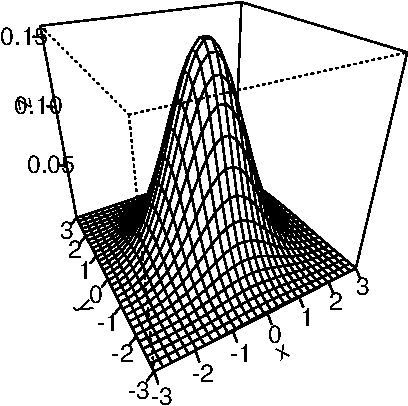
\includegraphics{_main_files/figure-latex/mvnorm-pdf-1.pdf}
\caption{\label{fig:mvnorm-pdf}\small A graph of a bivariate normal PDF.}
\end{figure}



\section{Bivariate Transformations of Random
Variables}\label{sec-transformations-multivariate}

We studied in Section \ref{sec-functions-of-continuous} how to find the
PDF of \(Y=g(X)\) given the PDF of \(X\). But now we have two random
variables \(X\) and Y, with joint PDF \(f_{X,Y}\), and we would like to
consider the joint PDF of two new random variables

\begin{equation}
U=g(X,Y)\quad \mbox{and}\quad V=h(X,Y),
\end{equation}

where \(g\) and \(h\) are two given functions, typically ``nice'' in the
sense of Appendix \ref{sec-multivariable-calculus}.

Suppose that the transformation \((x,y)\longmapsto(u,v)\) is one-to-one.
Then an inverse transformation \(x=x(u,v)\) and \(y=y(u,v)\) exists, so
let \(\partial(x,y)/\partial(u,v)\) denote the Jacobian of the inverse
transformation. Then the joint PDF of \((U,V)\) is given by

\begin{equation}
f_{U,V}(u,v)=f_{X,Y}\left[x(u,v),\, y(u,v)\right]\left|\frac{\partial(x,y)}{\partial(u,v)}\right|,
\end{equation}

or we can rewrite more shortly as

\begin{equation}
\label{eq-biv-trans-pdf-short}
f_{U,V}(u,v)=f_{X,Y}(x,y)\left|\frac{\partial(x,y)}{\partial(u,v)}\right|.
\end{equation}

Take a moment and compare Equation \eqref{eq-biv-trans-pdf-short} to
Equation \eqref{eq-univ-trans-pdf-short}. Do you see the connection?

\bigskip

\begin{remark}
It is sometimes easier to \emph{postpone} solving for the inverse
transformation \(x=x(u,v)\) and \(y=y(u,v)\). Instead, leave the
transformation in the form \(u=u(x,y)\) and \(v=v(x,y)\) and calculate
the Jacobian of the \emph{original} transformation

\begin{equation}
\frac{\partial(u,v)}{\partial(x,y)}=\left|\begin{array}{cc}
\frac{\partial u}{\partial x} & \frac{\partial u}{\partial y}\\
\frac{\partial v}{\partial x} & \frac{\partial v}{\partial y}\end{array}\right|=\frac{\partial u}{\partial x}\frac{\partial v}{\partial y}-\frac{\partial u}{\partial y}\frac{\partial v}{\partial x}.
\end{equation}

Once this is known, we can get the PDF of \((U,V)\) by

\begin{equation}
f_{U,V}(u,v)=f_{X,Y}(x,y)\left|\frac{1}{\frac{\partial(u,v)}{\partial(x,y)}}\right|.
\end{equation}

In some cases there will be a cancellation and the work will be lot
shorter. Of course, it is not always true that

\begin{equation}
\label{eq-biv-jacob-recip}
\frac{\partial(x,y)}{\partial(u,v)}=\frac{1}{\frac{\partial(u,v)}{\partial(x,y)}},
\end{equation}

but for the well-behaved examples that we will see in this book it works
just fine\ldots{} do you see the connection between Equations
\eqref{eq-biv-jacob-recip} and \eqref{eq-univ-jacob-recip}?
\end{remark}

\bigskip

\BeginKnitrBlock{example}
\protect\hypertarget{ex:unnamed-chunk-224}{}{\label{ex:unnamed-chunk-224}}Let
\((X,Y)\sim\mathsf{mvnorm}(\mathtt{mean}=\mathbf{0}_{2\times1},\,\mathtt{sigma}=\mathbf{I}_{2\times2})\)
and consider the transformation

\begin{align*}
U= & \ 3X+4Y,\\
V= & \ 5X+6Y.
\end{align*}

We can solve the system of equations to find the inverse
transformations; they are

\begin{align*}
X= & -3U+2V,\\
Y= & \ \frac{5}{2}U-\frac{3}{2}V,
\end{align*}

in which case the Jacobian of the inverse transformation is
\[ \begin{vmatrix} -3 & 2\\ \frac{5}{2} & -\frac{3}{2} \end{vmatrix} = -3\left(-\frac{3}{2}\right)-2\left(\frac{5}{2}\right) = -\frac{1}{2}.\]
As \((x,y)\) traverses \(\mathbb{R}^{2}\), so too does \((u,v)\). Since
the joint PDF of \((X,Y)\) is \[
f_{X,Y}(x,y)=\frac{1}{2\pi}\exp\left\{ -\frac{1}{2}\left(x^{2}+y^{2}\right)\right\} ,\quad (x,y)\in\mathbb{R}^{2},
\] we get that the joint PDF of \((U,V)\) is

\begin{equation}
\label{eq-biv-norm-hidden}
f_{U,V}(u,v)=\frac{1}{2\pi}\exp\left\{ -\frac{1}{2}\left[\left(-3u+2v\right)^{2}+\left(\frac{5u-3v}{2}\right)^{2}\right]\right\} \cdot\frac{1}{2},\quad (u,v)\in\mathbb{R}^{2}.
\end{equation}
\EndKnitrBlock{example}

\bigskip

\begin{remark}
It may not be obvious, but Equation \eqref{eq-biv-norm-hidden} is the
PDF of a \(\mathsf{mvnorm}\) distribution. For a more general result see
Theorem \ref{thm:mvnorm-dist-matrix-prod}.
\end{remark}

\subsubsection{How to do it with R}\label{sub-bivariate-transf-r}

It is possible to do the computations above in R with the
\texttt{Ryacas} package. The package is an interface to the open-source
computer algebra system, ``Yacas''. The user installs Yacas, then
employs \texttt{Ryacas} to submit commands to Yacas, after which the
output is displayed in the R console.

There are not yet any examples of Yacas in this book, but there are
online materials to help the interested reader: see
\url{http://code.google.com/p/ryacas/} to get started.

\section{Remarks for the Multivariate
Case}\label{sec-remarks-for-the-multivariate}

There is nothing spooky about \(n\geq3\) random variables. We just have
a whole bunch of them: \(X_{1}\), \(X_{2}\),\ldots{}, \(X_{n}\), which
we can shorten to \(\mathbf{X}=(X_{1},X_{2},\ldots,X_{n})^{\mathrm{T}}\)
to make the formulas prettier (now may be a good time to check out
Appendix \ref{sec-linear-algebra}). For \(\mathbf{X}\) supported on the
set \(S_{\mathbf{X}}\), the joint PDF \(f_{\mathbf{X}}\) (if it exists)
satisfies

\begin{equation}
f_{\mathbf{X}}(\mathbf{x})>0,\quad \mbox{for }\mathbf{x}\in S_{\mathbf{X}},
\end{equation}

and

\begin{equation}
\int\!\!\!\int\cdots\int f_{\mathbf{X}}(\mathbf{x})\,\mathrm{d} x_{1}\mathrm{d} x_{2}\cdots\mathrm{d} x_{n}=1,
\end{equation}

or even shorter:
\(\int f_{\mathbf{X}}(\mathbf{x})\,\mathrm{d}\mathbf{x}=1\). The joint
CDF \(F_{\mathbf{X}}\) is defined by

\begin{equation}
F_{\mathbf{X}}(\mathbf{x})=\mathbb{P}(X_{1}\leq x_{1},\, X_{2}\leq x_{2},\ldots,\, X_{n}\leq x_{n}),
\end{equation}

for \(\mathbf{x}\in\mathbb{R}^{n}\). The expectation of a function
\(g(\mathbf{X})\) is defined just as we would imagine:

\begin{equation}
\mathbb{E} g(\mathbf{X})=\int g(\mathbf{x})\, f_{\mathbf{X}}(\mathbf{x})\,\mathrm{d}\mathbf{x}.
\end{equation}

provided the integral exists and is finite. And the moment generating
function in the multivariate case is defined by

\begin{eqnarray} 
M_{\mathbf{X}}(\mathbf{t}) & = & \mathbb{E}\exp\left\{ \mathbf{t}^{\mathrm{T}}\mathbf{X}\right\},
\end{eqnarray}

whenever the integral exists and is finite for all \(\mathbf{t}\) in a
neighborhood of \(\mathbf{0}_{\mathrm{n}\times1}\) (note that
\(\mathbf{t}^{\mathrm{T}}\mathbf{X}\) is shorthand for
\(t_{1}X_{1}+t_{2}X_{2}+\cdots+t_{n}X_{n}\)). The only difference in any
of the above for the discrete case is that integrals are replaced by
sums.

Marginal distributions are obtained by integrating out remaining
variables from the joint distribution. And even if we are given all of
the univariate marginals it is not enough to determine the joint
distribution uniquely.

We say that \(X_{1}\), \(X_{2}\), \ldots{}, \(X_{n}\) are \emph{mutually
independent} if their joint PDF factors into the product of the
marginals

\begin{equation}
f_{\mathbf{X}}(\mathbf{x})=f_{X_{1}}(x_{1})\, f_{X_{2}}(x_{2})\,\cdots\, f_{X_{n}}(x_{n}),
\end{equation}

for every \(\mathbf{x}\) in their joint support \(S_{\mathbf{X}}\), and
we say that \(X_{1}\), \(X_{2}\), \ldots{}, \(X_{n}\) are
\emph{exchangeable} if their joint PDF (or CDF) is a symmetric function
of its \(n\) arguments, that is, if

\begin{equation}
f_{\mathbf{X}}(\mathbf{x^{\ast}})=f_{\mathbf{X}}(\mathbf{x}),
\end{equation}

for any reordering (permutation) \(\mathbf{x^{\ast}}\) of the elements
of \(\mathbf{x}=(x_{1},x_{2},\ldots,x_{n})\) in the joint support.

\bigskip

\BeginKnitrBlock{proposition}
\protect\hypertarget{prp:mean-sd-lin-comb}{}{\label{prp:mean-sd-lin-comb}}Let
\(X_{1}\), \(X_{2}\), \ldots{}, \(X_{n}\) be independent with respective
population means \(\mu_{1}\), \(\mu_{2}\), \ldots{}, \(\mu_{n}\) and
standard deviations \(\sigma_{1}\), \(\sigma_{2}\), \ldots{},
\(\sigma_{n}\). For given constants \(a_{1}\), \(a_{2}\),
\ldots{},\(a_{n}\) define \(Y=\sum_{i=1}^{n}a_{i}X_{i}\). Then the mean
and standard deviation of \(Y\) are given by the formulas

\begin{equation}
\mu_{Y}=\sum_{i=1}^{n}a_{i}\mu_{i},\quad \sigma_{Y}=\left(\sum_{i=1}^{n}a_{i}^{2}\sigma_{i}^{2}\right)^{1/2}.
\end{equation}
\EndKnitrBlock{proposition}

\bigskip

\BeginKnitrBlock{proof}
\iffalse {Proof. } \fi The mean is easy: \[ \mathbb{E}
Y=\mathbb{E}\left(\sum_{i=1}^{n}a_{i}X_{i}\right)=\sum_{i=1}^{n}a_{i}\mathbb{E}
X_{i}=\sum_{i=1}^{n}a_{i}\mu_{i}.  \] The variance is not too difficult
to compute either. As an intermediate step, we calculate
\(\mathbb{E} Y^{2}\). \[ \mathbb{E}
Y^{2}=\mathbb{E}\left(\sum_{i=1}^{n}a_{i}X_{i}\right)^{2}=\mathbb{E}\left(\sum_{i=1}^{n}a_{i}^{2}X_{i}^{2}+2\sum_{i=1}^{n-1}\sum_{j=i+1}^{n}a_{i}a_{j}X_{i}X_{j}\right).
\] Using linearity of expectation the \(\mathbb{E}\) distributes through
the sums. Now \(\mathbb{E} X_{i}^{2}=\sigma_{i}^{2}+\mu_{i}^{2}\) and
\(\mathbb{E} X_{i}X_{j}=\mathbb{E} X_{i}\mathbb{E} X_{j}=\mu_{i}\mu_{j}\)
when \(i\neq j\) because of independence. Thus

\begin{eqnarray*}
\mathbb{E} Y^{2} & = & \sum_{i=1}^{n}a_{i}^{2}(\sigma_{i}^{2}+\mu_{i}^{2})+2\sum_{i=1}^{n-1}\sum_{j=i+1}^{n}a_{i}a_{j}\mu_{i}\mu_{j}\\
 & = & \sum_{i=1}^{n}a_{i}^{2}\sigma_{i}^{2}+\left(\sum_{i=1}^{n}a_{i}^{2}\mu_{i}^{2}+2\sum_{i=1}^{n-1}\sum_{j=i+1}^{n}a_{i}a_{j}\mu_{i}\mu_{j}\right)
\end{eqnarray*}

To complete the proof, note that the expression in the parentheses is
exactly \(\left(\mathbb{E} Y\right)^{2}\), and recall the identity
\(\sigma_{Y}^{2}=\mathbb{E} Y^{2}-\left(\mathbb{E} Y\right)^{2}\).
\EndKnitrBlock{proof}

There is a corresponding statement of Fact
\ref{fac-indep-then-function-indep} for the multivariate case. The proof
is also omitted here.

\begin{fact}
If \(\mathbf{X}\) and \(\mathbf{Y}\) are mutually independent random
vectors, then \(u(\mathbf{X})\) and \(v(\mathbf{Y})\) are independent
for any functions \(u\) and \(v\).
\end{fact}

Bruno de Finetti was a strong proponent of the subjective approach to
probability. He proved an important theorem in 1931 which illuminates
the link between exchangeable random variables and independent random
variables. Here it is in one of its simplest forms.

\bigskip

\BeginKnitrBlock{theorem}[De Finetti's Theorem]
\protect\hypertarget{thm:unnamed-chunk-228}{}{\label{thm:unnamed-chunk-228}
\iffalse (De Finetti's Theorem) \fi }Let \(X_{1}\), \(X_{2}\), \ldots{}
be a sequence of \(\mathsf{binom}(\mathtt{size}=1,\,\mathtt{prob}=p)\)
random variables such that \((X_{1},\ldots,X_{k})\) are exchangeable for
every \(k\). Then there exists a random variable \(\Theta\) with support
\([0,1]\) and PDF \(f_{\Theta}(\theta)\) such that

\begin{equation}
\label{eq-definetti-binary}
\mathbb{P}(X_{1}=x_{1},\ldots,\, X_{k}=x_{k})=\int_{0}^{1}\theta^{\sum x_{i}}(1-\theta)^{k-\sum x_{i}}\, f_{\Theta}(\theta)\,\mathrm{d}\theta,
\end{equation}

for all \(x_{i}=0,\,1\), \(i=1,\,2,\ldots,k\).
\EndKnitrBlock{theorem}

To get a handle on the intuitive content de Finetti's theorem, imagine
that we have a \emph{bunch} of coins in our pocket with each having its
own unique value of \(\theta=\mathbb{P}(\mbox{Heads})\). We reach into
our pocket and select a coin at random according to some probability --
say, \(f_{\Theta}(\theta)\). We take the randomly selected coin and flip
it \(k\) times.

Think carefully: the conditional probability of observing a sequence
\(X_{1}=x_{1},\ldots,\, X_{k}=x_{k}\), given a specific coin \(\theta\)
would just be \(\theta^{\sum x_{i}}(1-\theta)^{k-\sum x_{i}}\), because
the coin flips are an independent sequence of Bernoulli trials. But the
coin is random, so the Theorem of Total Probability says we can get the
\emph{unconditional} probability
\(\mathbb{P}(X_{1}=x_{1},\ldots,\, X_{k}=x_{k})\) by adding up terms
that look like

\begin{equation}
\theta^{\sum x_{i}}(1-\theta)^{k-\sum x_{i}}\, f_{\Theta}(\theta),
\end{equation}

where we sum over all possible coins. The right-hand side of Equation
\eqref{eq-definetti-binary} is a sophisticated way to denote this
process.

Of course, the integral's value does not change if we jumble the
\(x_{i}\)'s, so \((X_{1},\ldots,X_{k})\) are clearly exchangeable. The
power of de Finetti's Theorem is that \emph{every} infinite binary
exchangeable sequence can be written in the above form.

The connection to subjective probability: our prior information about
\(\theta\) corresponds to \(f_{\Theta}(\theta)\) and the likelihood of
the sequence \(X_{1}=x_{1},\ldots,\, X_{k}=x_{k}\) (conditional on
\(\theta\)) corresponds to
\(\theta^{\sum x_{i}}(1-\theta)^{k-\sum x_{i}}\). Compare Equation
\eqref{eq-definetti-binary} to Section \ref{sec-Bayes-Rule} and Section
\ref{sec-conditional-distributions}.

The multivariate normal distribution immediately generalizes from the
bivariate case. If the matrix \(\Sigma\) is nonsingular then the joint
PDF of
\(\mathbf{X}\sim\mathsf{mvnorm}(\mathtt{mean}=\upmu,\,\mathtt{sigma}=\Sigma)\)
is

\begin{equation}
f_{\mathbf{X}}(\mathbf{x})=\frac{1}{(2\pi)^{n/2}\left|\Sigma\right|^{1/2}}\exp\left\{ -\frac{1}{2}\left(\mathbf{x}-\upmu\right)^{\top}\Sigma^{-1}\left(\mathbf{x}-\upmu\right)\right\},
\end{equation}

and the MGF is

\begin{equation}
M_{\mathbf{X}}(\mathbf{t})=\exp\left\{ \upmu^{\top}\mathbf{t}+\frac{1}{2}\mathbf{t}^{\top}\Sigma\mathbf{t}\right\}.
\end{equation}

We will need the following in Chapter
\ref{cha-multiple-linear-regression}.

\bigskip

\BeginKnitrBlock{theorem}
\protect\hypertarget{thm:mvnorm-dist-matrix-prod}{}{\label{thm:mvnorm-dist-matrix-prod}}If
\(\mathbf{X} \sim \mathsf{mvnorm}(\mathtt{mean} = \upmu, \, \mathtt{sigma} = \Sigma)\)
and \(\mathbf{A}\) is any matrix, then the random vector
\(\mathbf{Y}=\mathbf{AX}\) is distributed

\begin{equation}
\mathbf{Y}\sim\mathsf{mvnorm}(\mathtt{mean}=\mathbf{A}\upmu,\,\mathtt{sigma}=\mathbf{A}\Sigma\mathbf{A}^{\mathrm{T}}).
\end{equation}
\EndKnitrBlock{theorem}

\bigskip

\BeginKnitrBlock{proof}
\iffalse {Proof. } \fi Look at the MGF of \(\mathbf{Y}\):

\begin{eqnarray*}
M_{\mathbf{Y}}(\mathbf{t}) & = & \mathbb{E}\,\exp\left\{ \mathbf{t}^{\mathrm{T}}(\mathbf{AX})\right\} ,\\
 & = & \mathbb{E}\,\exp\left\{ (\mathbf{A}^{\mathrm{T}}\mathbf{t})^{\mathrm{T}}\mathbf{X}\right\} ,\\
 & = & \exp\left\{ \upmu^{\mathrm{T}}(\mathbf{A}^{\top}\mathbf{t})+\frac{1}{2}(\mathbf{A}^{\mathrm{T}}\mathbf{t})^{\mathrm{T}}\Sigma(\mathbf{A}^{\mathrm{T}}\mathbf{t})\right\} ,\\
 & = & \exp\left\{ \left(\mathbf{A}\upmu\right)^{\mathrm{T}}\mathbf{t}+\frac{1}{2}\mathbf{t}^{\mathrm{T}}\left(\mathbf{A}\Sigma\mathbf{A}^{\mathrm{T}}\right)\mathbf{t}\right\},
\end{eqnarray*}

and the last expression is the MGF of an
\(\mathsf{mvnorm}(\mathtt{mean}=\mathbf{A}\upmu,\,\mathtt{sigma}=\mathbf{A}\Sigma\mathbf{A}^{\mathrm{T}})\)
distribution.
\EndKnitrBlock{proof}

\section{The Multinomial Distribution}\label{sec-multinomial}

We sample \(n\) times, with replacement, from an urn that contains balls
of \(k\) different types. Let \(X_{1}\) denote the number of balls in
our sample of type 1, let \(X_{2}\) denote the number of balls of type
2, \ldots{}, and let \(X_{k}\) denote the number of balls of type \(k\).
Suppose the urn has proportion \(p_{1}\) of balls of type 1, proportion
\(p_{2}\) of balls of type 2, \ldots{}, and proportion \(p_{k}\) of
balls of type \(k\). Then the joint PMF of \((X_{1},\ldots,X_{k})\) is

\begin{eqnarray}
f_{X_{1},\ldots,X_{k}}(x_{1},\ldots,x_{k}) & = & {n \choose x_{1}\, x_{2}\,\cdots\, x_{k}}\, p_{1}^{x_{1}}p_{2}^{x_{2}}\cdots p_{k}^{x_{k}},
\end{eqnarray}

for \((x_{1},\ldots,x_{k})\) in the joint support
\(S_{X_{1},\ldots X_{K}}\). We write

\begin{equation}
(X_{1},\ldots,X_{k})\sim\mathsf{multinom}(\mathtt{size}=n,\,\mathtt{prob}=\mathbf{p}_{\mathrm{k}\times1}).
\end{equation}

Several comments are in order. First, the joint support set
\(S_{X_{1},\ldots X_{K}}\) contains all nonnegative integer \(k\)-tuples
\((x_{1},\ldots,x_{k})\) such that \(x_{1}+x_{2}+\cdots+x_{k}=n\). A
support set like this is called a \emph{simplex}. Second, the
proportions \(p_{1}\), \(p_{2}\), \ldots{}, \(p_{k}\) satisfy
\(p_{i}\geq0\) for all \(i\) and \(p_{1}+p_{2}+\cdots+p_{k}=1\).
Finally, the symbol

\begin{equation}
{n \choose x_{1}\, x_{2}\,\cdots\, x_{k}}=\frac{n!}{x_{1}!\, x_{2}!\,\cdots x_{k}!}
\end{equation}

is called a \emph{multinomial coefficient} which generalizes the notion
of a binomial coefficient we saw in Equation
\eqref{eq-binomial-coefficient}.

The form and notation we have just described matches the R usage but is
not standard among other texts. Most other books use the above for a
\(k-1\) dimension multinomial distribution, because the linear
constraint \(x_{1}+x_{2}+\cdots+x_{k}=n\) means that once the values of
\(X_{1}\), \(X_{2}\), \ldots{}, \(X_{k-1}\) are known the final value
\(X_{k}\) is determined, not random. Another term used for this is a
\emph{singular} distribution.

For the most part we will ignore these difficulties, but the careful
reader should keep them in mind. There is not much of a difference in
practice, except that below we will use a two-dimensional support set
for a three-dimension multinomial distribution. See Figure
\ref{fig:multinom-pmf2}.

When \(k=2\), we have \(x_{1}=x\) and \(x_{2}=n-x\), we have \(p_{1}=p\)
and \(p_{2}=1-p\), and the multinomial coefficient is literally a
binomial coefficient. In the previous notation we have thus shown that
the
\(\mathsf{multinom}(\mathtt{size}=n,\,\mathtt{prob}=\mathbf{p}_{2\times1})\)
distribution is the same as a
\(\mathsf{binom}(\mathtt{size}=n,\,\mathtt{prob}=p)\) distribution.

\bigskip

\BeginKnitrBlock{example}[Dinner with Barack Obama]
\protect\hypertarget{ex:unnamed-chunk-230}{}{\label{ex:unnamed-chunk-230}
\iffalse (Dinner with Barack Obama) \fi }During the 2008 U.S.
presidential primary, Barack Obama offered to have dinner with three
randomly selected monetary contributors to his campaign. Imagine the
thousands of people in the contributor database. For the sake of
argument, Suppose that the database was approximately representative of
the U.S. population as a whole, Suppose Barack Obama wants to have
\url{http://pewresearch.org/pubs/773/fewer-voters-identify-as-republicans}
with 36 democrats, 27 republicans, and 37 independents.
\EndKnitrBlock{example}

BLANK

\bigskip

\begin{remark}
Here are some facts about the multinomial distribution.

\begin{enumerate}
\def\labelenumi{\arabic{enumi}.}
\tightlist
\item
  The expected value of \((X_{1},\, X_{2},\,\ldots,\, X_{k})\) is
  \(n\mathbf{p}_{k\times1}\).
\item
  The variance-covariance matrix \(\Sigma\) is symmetric with diagonal
  entries \(\sigma_{i}^{2}=np_{i}(1-p_{i})\), \(i=1,\,2,\,\ldots,\, k\)
  and off-diagonal entries \(\mbox{Cov}(X_{i},\, X_{j})=-np_{i}p_{j}\),
  for \(i\neq j\). The correlation between \(X_{i}\) and \(X_{j}\) is
  therefore
  \(\mbox{Corr}(X_{i},\,  X_{j})=-\sqrt{p_{i}p_{j}/(1-p_{i})(1-p_{j})}\).
\item
  The marginal distribution of \((X_{1},\, X_{2},\,\ldots,\,  X_{k-1})\)
  is
  \(\mathsf{multinom}(\mathtt{size}=n,\,\mathtt{prob}=\mathbf{p}_{(k-1)\times1})\)
  with

  \begin{equation}
     \mathbf{p}_{(k-1)\times1}=\left(p_{1},\, p_{2},\,\ldots,\, p_{k-2},\, p_{k-1}+p_{k}\right),
     \end{equation}

  and in particular,
  \(X_{i}\sim\mathsf{binom}(\mathtt{size}=n,\,\mathtt{prob}=p_{i})\).
\end{enumerate}
\end{remark}

\subsection{How to do it with R}\label{how-to-do-it-with-r-23}

There is support for the multinomial distribution in base R, namely in
the \texttt{stats} package \autocite{stats}. The \texttt{dmultinom}
function represents the PMF and the \texttt{rmultinom} function
generates random variates.

\begin{Shaded}
\begin{Highlighting}[]
\NormalTok{tmp <-}\StringTok{ }\KeywordTok{t}\NormalTok{(}\KeywordTok{xsimplex}\NormalTok{(}\DecValTok{3}\NormalTok{, }\DecValTok{6}\NormalTok{))}
\NormalTok{p <-}\StringTok{ }\KeywordTok{apply}\NormalTok{(tmp, }\DataTypeTok{MARGIN =} \DecValTok{1}\NormalTok{, }\DataTypeTok{FUN =} \NormalTok{dmultinom, }\DataTypeTok{prob =} \KeywordTok{c}\NormalTok{(}\DecValTok{36}\NormalTok{,}\DecValTok{27}\NormalTok{,}\DecValTok{37}\NormalTok{))}
\NormalTok{S <-}\StringTok{ }\KeywordTok{probspace}\NormalTok{(tmp, }\DataTypeTok{probs =} \NormalTok{p)}
\NormalTok{ProbTable <-}\StringTok{ }\KeywordTok{xtabs}\NormalTok{(probs ~}\StringTok{ }\NormalTok{X1 +}\StringTok{ }\NormalTok{X2, }\DataTypeTok{data =} \NormalTok{S)}
\KeywordTok{round}\NormalTok{(ProbTable, }\DecValTok{3}\NormalTok{)}
\end{Highlighting}
\end{Shaded}

\begin{verbatim}
   X2
X1      0     1     2     3     4     5     6
  0 0.003 0.011 0.020 0.020 0.011 0.003 0.000
  1 0.015 0.055 0.080 0.058 0.021 0.003 0.000
  2 0.036 0.106 0.116 0.057 0.010 0.000 0.000
  3 0.047 0.103 0.076 0.018 0.000 0.000 0.000
  4 0.034 0.050 0.018 0.000 0.000 0.000 0.000
  5 0.013 0.010 0.000 0.000 0.000 0.000 0.000
  6 0.002 0.000 0.000 0.000 0.000 0.000 0.000
\end{verbatim}

BLANK

Do some examples of \texttt{rmultinom}.

Another way to do the plot is with the \texttt{scatterplot3d} function
in the \texttt{scatterplot3d} package \autocite{scatterplot3d}. It looks
like this:

\begin{Shaded}
\begin{Highlighting}[]
\KeywordTok{library}\NormalTok{(}\StringTok{"scatterplot3d"}\NormalTok{)}
\NormalTok{X <-}\StringTok{ }\KeywordTok{t}\NormalTok{(}\KeywordTok{as.matrix}\NormalTok{(}\KeywordTok{expand.grid}\NormalTok{(}\DecValTok{0}\NormalTok{:}\DecValTok{6}\NormalTok{, }\DecValTok{0}\NormalTok{:}\DecValTok{6}\NormalTok{)))}
\NormalTok{X <-}\StringTok{ }\NormalTok{X[, }\KeywordTok{colSums}\NormalTok{(X) <=}\StringTok{ }\DecValTok{6} \NormalTok{]; X <-}\StringTok{ }\KeywordTok{rbind}\NormalTok{(X, }\DecValTok{6} \NormalTok{-}\StringTok{ }\KeywordTok{colSums}\NormalTok{(X))}
\NormalTok{Z <-}\StringTok{ }\KeywordTok{round}\NormalTok{(}\KeywordTok{apply}\NormalTok{(X, }\DecValTok{2}\NormalTok{, function(x) }\KeywordTok{dmultinom}\NormalTok{(x, }\DataTypeTok{prob =} \DecValTok{1}\NormalTok{:}\DecValTok{3}\NormalTok{)), }\DecValTok{3}\NormalTok{)}
\NormalTok{A <-}\StringTok{ }\KeywordTok{data.frame}\NormalTok{(}\DataTypeTok{x =} \NormalTok{X[}\DecValTok{1}\NormalTok{, ], }\DataTypeTok{y =} \NormalTok{X[}\DecValTok{2}\NormalTok{, ], }\DataTypeTok{probability =} \NormalTok{Z)}
\KeywordTok{scatterplot3d}\NormalTok{(A, }\DataTypeTok{type =} \StringTok{"h"}\NormalTok{, }\DataTypeTok{lwd =} \DecValTok{3}\NormalTok{, }\DataTypeTok{box =} \OtherTok{FALSE}\NormalTok{)}
\end{Highlighting}
\end{Shaded}

The \texttt{scatterplot3d} graph looks better in this example, but the
code is more difficult to understand. And with \texttt{cloud} one can
easily do conditional plots of the form
\texttt{cloud(z\ \textasciitilde{}\ x\ +\ y\ \textbar{}\ f)}, where
\texttt{f} is a factor.

\begin{Shaded}
\begin{Highlighting}[]
\KeywordTok{cloud}\NormalTok{(probs ~}\StringTok{ }\NormalTok{X1 +}\StringTok{ }\NormalTok{X2, }\DataTypeTok{data =} \NormalTok{S, }\DataTypeTok{type =} \KeywordTok{c}\NormalTok{(}\StringTok{"p"}\NormalTok{,}\StringTok{"h"}\NormalTok{), }\DataTypeTok{lwd =} \DecValTok{2}\NormalTok{, }
            \DataTypeTok{pch =} \DecValTok{16}\NormalTok{, }\DataTypeTok{cex =} \FloatTok{1.5}\NormalTok{, }\DataTypeTok{screen =} \KeywordTok{list}\NormalTok{(}\DataTypeTok{z =} \DecValTok{15}\NormalTok{, }\DataTypeTok{x =} \NormalTok{-}\DecValTok{70}\NormalTok{))}
\end{Highlighting}
\end{Shaded}

\begin{figure}[htbp]
\centering
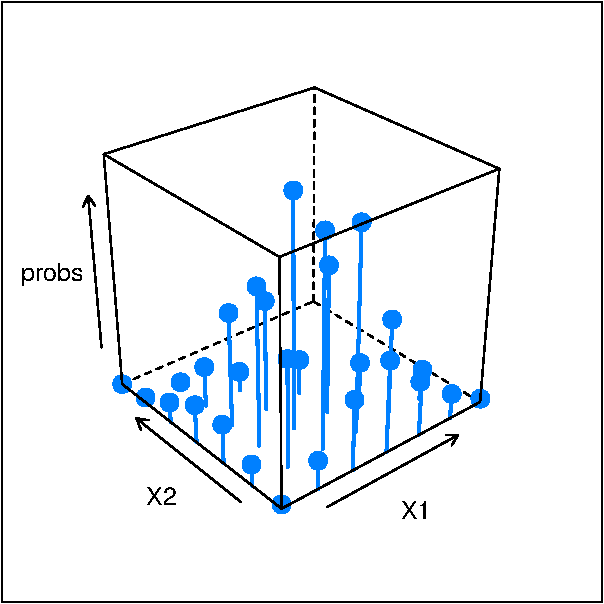
\includegraphics{_main_files/figure-latex/multinom-pmf2-1.pdf}
\caption{\label{fig:multinom-pmf2}\small A plot of a multinomial PMF.}
\end{figure}



\section{Exercises}\label{exercises-3}

\begin{xca}
Prove that
\(\mbox{Cov}(X,Y)=\mathbb{E}(XY)-(\mathbb{E} X)(\mathbb{E} Y).\)
\end{xca}

\begin{xca}
Suppose \(X\sim\mathsf{chisq}(\mathtt{df}=p_{1})\) and
\(Y\sim\mathsf{chisq}(\mathtt{df}=p_{2})\) are independent. Find the
distribution of \(X+Y\) (you may want to refer to Equation
\eqref{eq-mgf-chisq}).
\end{xca}

\bigskip

\begin{xca}
Show that when \(X\) and \(Y\) are independent the MGF of \(X-Y\) is
\(M_{X}(t)M_{Y}(-t)\). Use this to find the distribution of \(X-Y\) when
\(X\sim\mathsf{norm}(\mathtt{mean}=\mu_{1},\,\mathtt{sd}=\sigma_{1})\)
and
\(Y\sim\mathsf{norm}(\mathtt{mean}=\mu_{2},\,\mathtt{sd}=\sigma_{2})\)
are independent.
\end{xca}

\chapter{Simple Linear Regression}\label{cha-simple-linear-regression}

\textbf{What do I want them to know?}

\begin{itemize}
\tightlist
\item
  basic philosophy of SLR and the regression assumptions
\item
  point and interval estimation of the model parameters, and how to use
  it to make predictions
\item
  point and interval estimation of future observations from the model
\item
  regression diagnostics, including \(R^{2}\) and basic residual
  analysis
\item
  the concept of influential versus outlying observations, and how to
  tell the difference
\end{itemize}

\section{Basic Philosophy}\label{sec-basic-philosophy}

Here we have two variables \(X\) and \(Y\). For our purposes, \(X\) is
not random (so we will write \(x\)), but \(Y\) is random. We believe
that \(Y\) depends in \emph{some} way on \(x\). Some typical examples of
\((x,Y)\) pairs are

\begin{itemize}
\tightlist
\item
  \(x =\) study time and \(Y =\) score on a test.
\item
  \(x =\) height and \(Y =\) weight.
\item
  \(x =\) smoking frequency and \(Y =\) age of first heart attack.
\end{itemize}

Given information about the relationship between \(x\) and \(Y\), we
would like to \emph{predict} future values of \(Y\) for particular
values of \(x\). This turns out to be a difficult problem\footnote{We
  can find solutions of the normal equations even when
  \(\mathbf{X}^{\mathrm{T}}\mathbf{X}\) is not of full rank, but the
  topic falls outside the scope of this book. The interested reader can
  consult an advanced text such as Rao \autocite{Rao1999}.}, so instead
we first tackle an easier problem: we estimate \(\mathbb{E}Y\). How can
we accomplish this? Well, we know that \(Y\) depends somehow on \(x\),
so it stands to reason that

\begin{equation}
\mathbb{E} Y = \mu(x),\ \mbox{a function of }x.
\end{equation}

But we should be able to say more than that. To focus our efforts we
impose some structure on the functional form of \(\mu\). For instance,

\begin{itemize}
\tightlist
\item
  if \(\mu(x)=\beta_{0}+\beta_{1}x\), we try to estimate \(\beta_{0}\)
  and \(\beta_{1}\).
\item
  if \(\mu(x) = \beta_{0} + \beta_{1}x + \beta_{2}x^{2}\), we try to
  estimate \(\beta_{0}\), \(\beta_{1}\), and \(\beta_{2}\).
\item
  if \(\mu(x) = \beta_{0} \mathrm{e}^{\beta_{1}x}\), we try to estimate
  \(\beta_{0}\) and \(\beta_{1}\).
\end{itemize}

This helps us in the sense that we concentrate on the estimation of just
a few parameters, \(\beta_{0}\) and \(\beta_{1}\), say, rather than some
nebulous function. Our \emph{modus operandi} is simply to perform the
random experiment \(n\) times and observe the \(n\) ordered pairs of
data \((x_{1},Y_{1}),\ (x_{2},Y_{2}),\ \ldots,(x_{n},Y_{n})\). We use
these \(n\) data points to estimate the parameters.

More to the point, there are \emph{three simple linear regression} (SLR)
assumptions \index{regression assumptions} that will form the basis for
the rest of this chapter:

\bigskip

\begin{assumption}
We assume that \(\mu\) is a linear function of \(x\), that is,

\begin{equation}
\mu(x)=\beta_{0}+\beta_{1}x,
\end{equation}

where \(\beta_{0}\) and \(\beta_{1}\) are unknown constants to be
estimated. \bigskip
\end{assumption}\begin{assumption}
We further assume that \(Y_{i}\) is \(\mu(x_{i})\), a ``signal'', plus
some ``error'' (represented by the symbol \(\epsilon_{i}\)):

\begin{equation}
Y_{i} = \beta_{0} + \beta_{1}x_{i} + \epsilon_{i}, \quad i = 1,2,\ldots,n.
\end{equation}
\end{assumption}

\bigskip

\begin{assumption}
We lastly assume that the errors are IID normal with mean 0 and variance
\(\sigma^{2}\):

\begin{equation}
\epsilon_{1},\epsilon_{2},\ldots,\epsilon_{n}\sim\mathsf{norm}(\mathtt{mean}=0,\,\mathtt{sd}=\sigma).
\end{equation}
\end{assumption}

\bigskip

\begin{rem}
We assume both the normality of the errors \(\epsilon\) and the
linearity of the mean function \(\mu\). Recall from Proposition
\ref{pro:mvnorm-cond-dist} of Chapter
\ref{cha-multivariable-distributions} that if
\((X,Y) \sim \mathsf{mvnorm}\) then the mean of \(Y|x\) is a linear
function of \(x\). This is not a coincidence. In more advanced classes
we study the case that both \(X\) and \(Y\) are random, and in
particular, when they are jointly normally distributed.
\end{rem}

\subsection{What does it all mean?}\label{what-does-it-all-mean}

See Figure \ref{fig:philosophy}. Shown in the figure is a solid line,
the regression line \index{regression line} \(\mu\), which in this
display has slope 0.5 and \emph{y}-intercept 2.5, that is,
\(\mu(x)=2.5 + 0.5x\). The intuition is that for each given value of
\(x\), we observe a random value of \(Y\) which is normally distributed
with a mean equal to the height of the regression line at that \(x\)
value. Normal densities are superimposed on the plot to drive this point
home; in principle, the densities stand outside of the page,
perpendicular to the plane of the paper. The figure shows three such
values of \(x\), namely, \(x = 1\), \(x = 2.5\), and \(x = 4\). Not only
do we assume that the observations at the three locations are
independent, but we also assume that their distributions have the same
spread. In mathematical terms this means that the normal densities all
along the line have identical standard deviations -- there is no
``fanning out'' or ``scrunching in'' of the normal densities as \(x\)
increases\footnote{We are taking great leaps over the mathematical
  details. In particular, we have yet to show that \(s^{2}\) has a
  chi-square distribution and we have not even come close to showing
  that \(b_{i}\) and \(s_{b_{i}}\) are independent. But these are
  entirely outside the scope of the present book and the reader may rest
  assured that the proofs await in later classes. See C.R. Rao for more.}.

\begin{figure}[htbp]
\centering
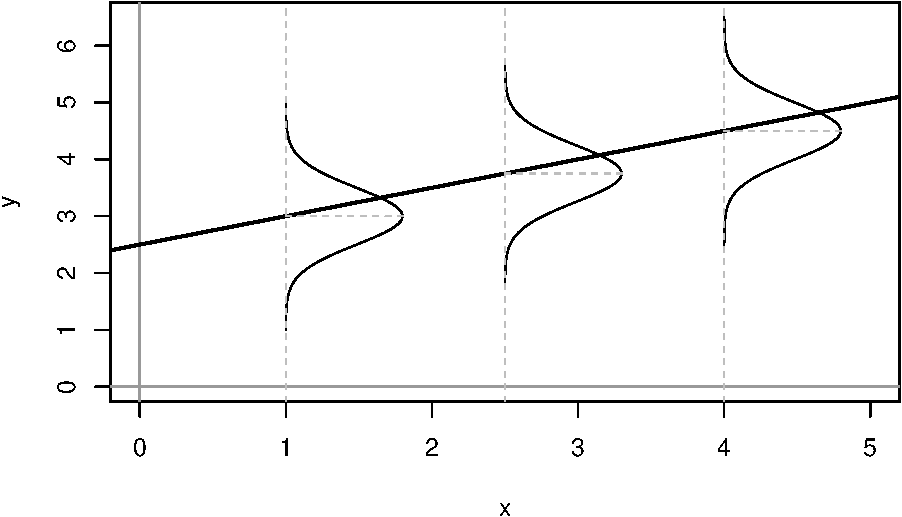
\includegraphics{_main_files/figure-latex/philosophy-1.pdf}
\caption{\label{fig:philosophy}\small Philosophical foundations of SLR.}
\end{figure}



\bigskip

\BeginKnitrBlock{example}[Speed and stopping distance of cars]
\protect\hypertarget{ex:unnamed-chunk-242}{}{\label{ex:unnamed-chunk-242}
\iffalse (Speed and stopping distance of cars) \fi }We will use the data
frame \texttt{cars} \index{Data
sets!cars@\texttt{cars}} from the \texttt{datasets} package
\autocite{datasets}. It has two variables: \texttt{speed} and
\texttt{dist}. We can take a look at some of the values in the data
frame:
\EndKnitrBlock{example}

\begin{Shaded}
\begin{Highlighting}[]
\KeywordTok{head}\NormalTok{(cars)}
\end{Highlighting}
\end{Shaded}

\begin{verbatim}
  speed dist
1     4    2
2     4   10
3     7    4
4     7   22
5     8   16
6     9   10
\end{verbatim}

The \texttt{speed} represents how fast the car was going (\(x\)) in
miles per hour and \texttt{dist} (\(Y\)) measures how far it took the
car to stop, in feet. We first make a simple scatterplot of the data.

\begin{Shaded}
\begin{Highlighting}[]
\KeywordTok{plot}\NormalTok{(dist ~}\StringTok{ }\NormalTok{speed, }\DataTypeTok{data =} \NormalTok{cars)}
\end{Highlighting}
\end{Shaded}

\begin{figure}[htbp]
\centering
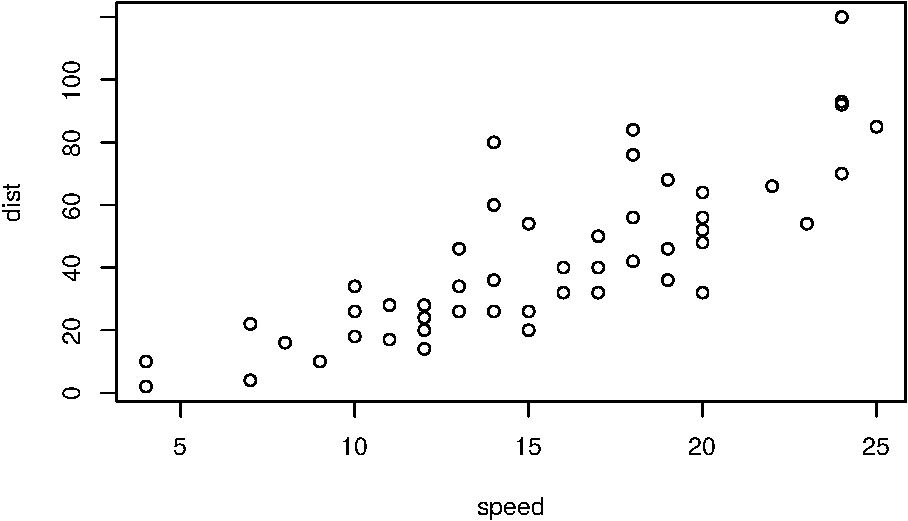
\includegraphics{_main_files/figure-latex/carscatter-1.pdf}
\caption{\label{fig:carscatter}\small A scatterplot of \texttt{dist} versus
\texttt{speed} for the \texttt{cars} data. There is clearly an upward
trend to the plot which is approximately linear.}
\end{figure}





You can see the output in Figure \ref{fig:carscatter}, which was
produced by the following code.

\begin{Shaded}
\begin{Highlighting}[]
\KeywordTok{plot}\NormalTok{(dist ~}\StringTok{ }\NormalTok{speed, }\DataTypeTok{data =} \NormalTok{cars)}
\end{Highlighting}
\end{Shaded}

There is a pronounced upward trend to the data points, and the pattern
looks approximately linear. There does not appear to be substantial
fanning out of the points or extreme values.

\section{Estimation}\label{sec-slr-estimation}

\subsection{Point Estimates of the
Parameters}\label{sub-point-estimate-mle-slr}

Where is \(\mu(x)\)? In essence, we would like to ``fit'' a line to the
points. But how do we determine a ``good'' line? Is there a \emph{best}
line? We will use maximum likelihood \index{maximum likelihood} to find
it. We know:

\begin{equation}
Y_{i} = \beta_{0} + \beta_{1}x_{i} + \epsilon_{i},\quad i=1,\ldots,n,
\end{equation}

where the \(\epsilon_{i}\) are IID
\(\mathsf{norm}(\mathtt{mean}=0,\,\mathtt{sd}=\sigma)\). Thus
\(Y_{i}\sim\mathsf{norm}(\mathtt{mean}=\beta_{0}+\beta_{1}x_{i},\,\mathtt{sd}=\sigma),\
i=1,\ldots,n\). Furthermore, \(Y_{1},\ldots,Y_{n}\) are independent --
but not identically distributed. The likelihood function
\index{likelihood function} is:

\begin{alignat}{1}
L(\beta_{0},\beta_{1},\sigma)= & \prod_{i=1}^{n}f_{Y_{i}}(y_{i}),\\
= & \prod_{i=1}^{n}(2\pi\sigma^{2})^{-1/2}\exp\left\{ \frac{-(y_{i}-\beta_{0}-\beta_{1}x_{i})^{2}}{2\sigma^{2}}\right\} ,\\
= & (2\pi\sigma^{2})^{-n/2}\exp\left\{ \frac{-\sum_{i=1}^{n}(y_{i}-\beta_{0}-\beta_{1}x_{i})^{2}}{2\sigma^{2}}\right\} .
\end{alignat}

We take the natural logarithm to get

\begin{equation}
\label{eq-regML-lnL}
\ln L(\beta_{0},\beta_{1},\sigma)=-\frac{n}{2}\ln(2\pi\sigma^{2})-\frac{\sum_{i=1}^{n}(y_{i}-\beta_{0}-\beta_{1}x_{i})^{2}}{2\sigma^{2}}.
\end{equation}

We would like to maximize this function of \(\beta_{0}\) and
\(\beta_{1}\). See Appendix \ref{sec-multivariable-calculus} which tells
us that we should find critical points by means of the partial
derivatives. Let us start by differentiating with respect to
\(\beta_{0}\):

\begin{equation}
\frac{\partial}{\partial\beta_{0}}\ln L=0-\frac{1}{2\sigma^{2}}\sum_{i=1}^{n}2(y_{i}-\beta_{0}-\beta_{1}x_{i})(-1),
\end{equation}

and the partial derivative equals zero when
\(\sum_{i=1}^{n}(y_{i}-\beta_{0}-\beta_{1}x_{i}) = 0\), that is, when

\begin{equation}
\label{eq-regML-a}
n \beta_{0} + \beta_{1} \sum_{i=1}^{n} x_{i} = \sum_{i = 1}^{n}y_{i}.
\end{equation}

Moving on, we next take the partial derivative of \(\ln L\) (Equation
\eqref{eq-regML-lnL}) with respect to \(\beta_{1}\) to get

\begin{alignat}{1}
\frac{\partial}{\partial \beta_{1}} \ln L = \ & 0 - \frac{1}{2\sigma^{2}} \sum_{i=1}^{n} 2 (y_{i} - \beta_{0} - \beta_{1} x_{i})(-x_{i}),\\ = & \frac{1}{\sigma^{2}}\sum_{i = 1}^{n}\left(x_{i} y_{i} - \beta_{0}x_{i} - \beta_{1}x_{i}^{2}\right),
\end{alignat}

and this equals zero when the last sum equals zero, that is, when

\begin{equation}
\label{eq-regML-b}
\beta_{0} \sum_{i = 1}^{n}x_{i} + \beta_{1} \sum_{i = 1}^{n}x_{i}^{2} = \sum_{i = 1}^{n}x_{i}y_{i}.
\end{equation}

Solving the system of equations \eqref{eq-regML-a} and
\eqref{eq-regML-b}

\begin{eqnarray}
n\beta_{0} + \beta_{1}\sum_{i = 1}^{n}x_{i} & = & \sum_{i = 1}^{n}y_{i}\\
\beta_{0}\sum_{i = 1}^{n}x_{i}+\beta_{1}\sum_{i = 1}^{n}x_{i}^{2} & = & \sum_{i = 1}^{n}x_{i}y_{i}
\end{eqnarray}

for \(\beta_{0}\) and \(\beta_{1}\) (in Exercise
\ref{xca:find-mles-slr}) gives

\begin{equation}
\label{eq-regline-slope-formula}
\hat{\beta}_{1} = \frac{\sum_{i = 1}^{n}x_{i}y_{i} - \left.\left(\sum_{i = 1}^{n}x_{i}\right)\left(\sum_{i = 1}^{n}y_{i}\right)\right] n}{\sum_{i = 1}^{n}x_{i}^{2} - \left.\left(\sum_{i = 1}^{n}x_{i}\right)^{2}\right/ n}
\end{equation}

and

\begin{equation}
\hat{\beta}_{0} = \overline{y} - \hat{\beta}_{1}\overline{x}.
\end{equation}

The conclusion? To estimate the mean line

\begin{equation}
\mu(x) = \beta_{0} + \beta_{1}x,
\end{equation}

we use the ``line of best fit''

\begin{equation}
\hat{\mu}(x) = \hat{\beta}_{0} + \hat{\beta}_{1}x,
\end{equation}

where \(\hat{\beta}_{0}\) and \(\hat{\beta}_{1}\) are given as above.
For notation we will usually write \(b_{0} = \hat{\beta_{0}}\) and
\(b_{1}=\hat{\beta_{1}}\) so that \(\hat{\mu}(x) = b_{0} + b_{1}x\).

\bigskip

\begin{rem}
The formula for \(b_{1}\) in Equation \eqref{eq-regline-slope-formula}
gets the job done but does not really make any sense. There are many
equivalent formulas for \(b_{1}\) that are more intuitive, or at the
least are easier to remember. One of the author's favorites is

\begin{equation}
\label{eq-sample-correlation-formula} 
b_{1} = r\frac{s_{y}}{s_{x}},
\end{equation}

where \(r\), \(s_{y}\), and \(s_{x}\) are the sample correlation
coefficient and the sample standard deviations of the \(Y\) and \(x\)
data, respectively. See Exercise \ref{xca:show-alternate-slope-formula}.
Also, notice the similarity between Equation
\eqref{eq-sample-correlation-formula} and Equation
\eqref{eq-population-slope-slr}.
\end{rem}

\subsubsection{How to do it with R}\label{how-to-do-it-with-r-24}

Here we go. R will calculate the linear regression line with the
\texttt{lm} function. We will store the result in an object which we
will call \texttt{cars.lm}. Here is how it works:

\begin{Shaded}
\begin{Highlighting}[]
\NormalTok{cars.lm <-}\StringTok{ }\KeywordTok{lm}\NormalTok{(dist ~}\StringTok{ }\NormalTok{speed, }\DataTypeTok{data =} \NormalTok{cars)}
\end{Highlighting}
\end{Shaded}

The first part of the input to the \texttt{lm} function,
\texttt{dist\ \textasciitilde{}\ speed}, is a \emph{model formula}, read
like this: \texttt{dist} is described (or modeled) by \texttt{speed}.
The \texttt{data\ =\ cars} argument tells R where to look for the
variables quoted in the model formula. The output object
\texttt{cars.lm} contains a multitude of information. Let's first take a
look at the coefficients of the fitted regression line, which are
extracted by the \texttt{coef} function (alternatively, we could just
type \texttt{cars.lm} to see the same thing):

\begin{Shaded}
\begin{Highlighting}[]
\KeywordTok{coef}\NormalTok{(cars.lm)}
\end{Highlighting}
\end{Shaded}

\begin{verbatim}
(Intercept)       speed 
 -17.579095    3.932409 
\end{verbatim}

The parameter estimates \(b_{0}\) and \(b_{1}\) for the intercept and
slope, respectively, are shown above.

It is good practice to visually inspect the data with the regression
line added to the plot. To do this we first scatterplot the original
data and then follow with a call to the \texttt{abline} function. The
inputs to \texttt{abline} are the coefficients of \texttt{cars.lm}; see
Figure \ref{fig:carline}.

\begin{Shaded}
\begin{Highlighting}[]
\KeywordTok{plot}\NormalTok{(dist ~}\StringTok{ }\NormalTok{speed, }\DataTypeTok{data =} \NormalTok{cars, }\DataTypeTok{pch =} \DecValTok{16}\NormalTok{)}
\KeywordTok{abline}\NormalTok{(}\KeywordTok{coef}\NormalTok{(cars))}
\end{Highlighting}
\end{Shaded}

\begin{figure}[htbp]
\centering
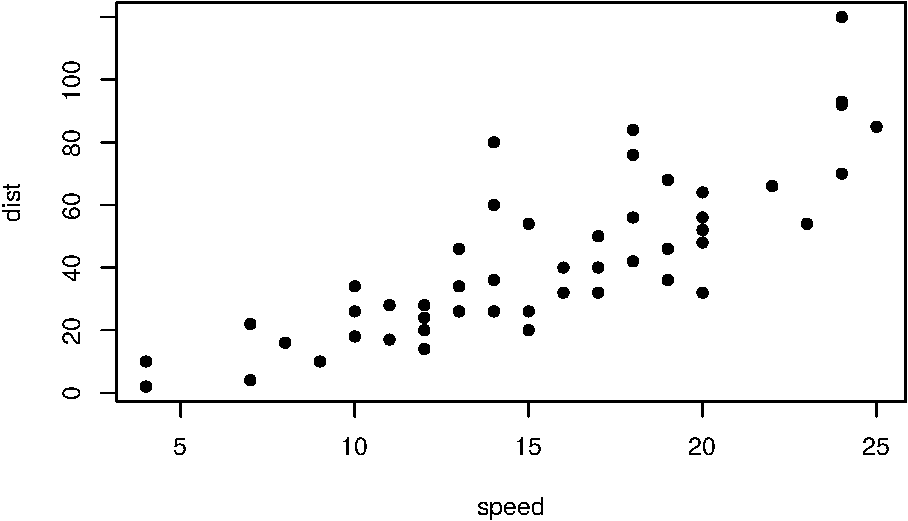
\includegraphics{_main_files/figure-latex/carline-1.pdf}
\caption{\label{fig:carline}(ref:carline)}
\end{figure}




To calculate points on the regression line we may simply plug the
desired \(x\) value(s) into \(\hat{\mu}\), either by hand, or with the
\texttt{predict} function. The inputs to \texttt{predict} are the fitted
linear model object, \texttt{cars.lm}, and the desired \(x\) value(s)
represented by a data frame. See the example below.

\bigskip

\BeginKnitrBlock{example}
\protect\hypertarget{ex:regline-cars-interpret}{}{\label{ex:regline-cars-interpret}}Using
the regression line for the \texttt{cars} data:
\EndKnitrBlock{example}

\begin{enumerate}
\def\labelenumi{\arabic{enumi}.}
\tightlist
\item
  What is the meaning of \(\mu(60) = \beta_{0} + \beta_{1}(8)\)? This
  represents the average stopping distance (in feet) for a car going 8
  mph.
\item
  Interpret the slope \(\beta_{1}\). The true slope \(\beta_{1}\)
  represents the increase in average stopping distance for each mile per
  hour faster that the car drives. In this case, we estimate the car to
  take approximately 3.93 additional feet to stop for each additional
  mph increase in speed.
\item
  Interpret the intercept \(\beta_{0}\). This would represent the mean
  stopping distance for a car traveling 0 mph (which our regression line
  estimates to be (-17.58. Of course, this interpretation does not make
  any sense for this example, because a car travelling 0 mph takes 0 ft
  to stop (it was not moving in the first place)! What went wrong?
  Looking at the data, we notice that the smallest speed for which we
  have measured data is 4 mph. Therefore, if we predict what would
  happen for slower speeds then we would be \emph{extrapolating}, a
  dangerous practice which often gives nonsensical results.
\end{enumerate}

\subsection{Point Estimates of the Regression
Line}\label{sub-slr-point-est-regline}

We said at the beginning of the chapter that our goal was to estimate
\(\mu = \mathbb{E} Y\), and the arguments in Section
\ref{sub-point-estimate-mle-slr} showed how to obtain an estimate
\(\hat{\mu}\) of \(\mu\) when the regression assumptions hold. Now we
will reap the benefits of our work in more ways than we previously
disclosed. Given a particular value \(x_{0}\), there are two values we
would like to estimate:

\begin{enumerate}
\def\labelenumi{\arabic{enumi}.}
\tightlist
\item
  the mean value of \(Y\) at \(x_{0}\), and
\item
  a future value of \(Y\) at \(x_{0}\). The first is a number,
  \(\mu(x_{0})\), and the second is a random variable, \(Y(x_{0})\), but
  our point estimate is the same for both: \(\hat{\mu}(x_{0})\).
\end{enumerate}

\bigskip

\BeginKnitrBlock{example}
\protect\hypertarget{ex:regline-cars-pe-8mph}{}{\label{ex:regline-cars-pe-8mph}}We
may use the regression line to obtain a point estimate of the mean
stopping distance for a car traveling 8 mph:
\(\hat{\mu}(15) = b_{0} + (8) (b_{1})\) which is approximately 13.88. We
would also use 13.88 as a point estimate for the stopping distance of a
future car traveling 8 mph.
\EndKnitrBlock{example}

Note that we actually have observed data for a car traveling 8 mph; its
stopping distance was 16 ft as listed in the fifth row of the
\texttt{cars} data (which we saw in Example
\ref{ex:speed-and-stopping}).

\begin{Shaded}
\begin{Highlighting}[]
\NormalTok{cars[}\DecValTok{5}\NormalTok{, ]}
\end{Highlighting}
\end{Shaded}

\begin{verbatim}
  speed dist
5     8   16
\end{verbatim}

There is a special name for estimates \(\hat{\mu}(x_{0})\) when (
x\_\{0\}) matches an observed value \(x_{i}\) from the data set. They
are called \emph{fitted values}, they are denoted by \(\hat{Y}_{1}\),
\(\hat{Y}_{2}\), \ldots{}, \(\hat{Y}_{n}\) (ignoring repetition), and
they play an important role in the sections that follow.

In an abuse of notation we will sometimes write \(\hat{Y}\) or
\(\hat{Y}(x_{0})\) to denote a point on the regression line even when
\(x_{0}\) does not belong to the original data if the context of the
statement obviates any danger of confusion.

We saw in Example \ref{ex:regline-cars-interpret} that spooky things can
happen when we are cavalier about point estimation. While it is usually
acceptable to predict/estimate at values of \(x_{0}\) that fall within
the range of the original \(x\) data, it is reckless to use
\(\hat{\mu}\) for point estimates at locations outside that range. Such
estimates are usually worthless. \emph{Do not extrapolate} unless there
are compelling external reasons, and even then, temper it with a good
deal of caution.

\subsubsection{How to do it with R}\label{how-to-do-it-with-r-25}

The fitted values are automatically computed as a byproduct of the model
fitting procedure and are already stored as a component of the
\texttt{cars.lm} object. We may access them with the \texttt{fitted}
function (we only show the first five entries):

\begin{Shaded}
\begin{Highlighting}[]
\KeywordTok{fitted}\NormalTok{(cars.lm)[}\DecValTok{1}\NormalTok{:}\DecValTok{5}\NormalTok{]}
\end{Highlighting}
\end{Shaded}

\begin{verbatim}
        1         2         3         4         5 
-1.849460 -1.849460  9.947766  9.947766 13.880175 
\end{verbatim}

Predictions at \(x\) values that are not necessarily part of the
original data are done with the \texttt{predict} function. The first
argument is the original \texttt{cars.lm} object and the second argument
\texttt{newdata} accepts a dataframe (in the same form that was used to
fit \texttt{cars.lm}) that contains the locations at which we are
seeking predictions. Let us predict the average stopping distances of
cars traveling 6 mph, 8 mph, and 21 mph:

\begin{Shaded}
\begin{Highlighting}[]
\KeywordTok{predict}\NormalTok{(cars.lm, }\DataTypeTok{newdata =} \KeywordTok{data.frame}\NormalTok{(}\DataTypeTok{speed =} \KeywordTok{c}\NormalTok{(}\DecValTok{6}\NormalTok{, }\DecValTok{8}\NormalTok{, }\DecValTok{21}\NormalTok{)))}
\end{Highlighting}
\end{Shaded}

\begin{verbatim}
        1         2         3 
 6.015358 13.880175 65.001489 
\end{verbatim}

Note that there were no observed cars that traveled 6 mph or 21 mph.
Also note that our estimate for a car traveling 8 mph matches the value
we computed by hand in Example \ref{ex:regline-cars-pe-8mph}.

\subsection{Mean Square Error and Standard
Error}\label{mean-square-error-and-standard-error}

To find the MLE of \(\sigma^{2}\) we consider the partial derivative

\begin{equation}
\frac{\partial}{\partial\sigma^{2}}\ln L=\frac{n}{2\sigma^{2}}-\frac{1}{2(\sigma^{2})^{2}}\sum_{i=1}^{n}(y_{i}-\beta_{0}-\beta_{1}x_{i})^{2},
\end{equation}

and after plugging in \(\hat{\beta}_{0}\) and \(\hat{\beta}_{1}\) and
setting equal to zero we get

\begin{equation}
\hat{\sigma^{2}}=\frac{1}{n}\sum_{i=1}^{n}(y_{i}-\hat{\beta}_{0}-\hat{\beta}_{1}x_{i})^{2}=\frac{1}{n}\sum_{i=1}^{n}[y_{i}-\hat{\mu}(x_{i})]^{2}.
\end{equation}

We write \(\hat{Yi}=\hat{\mu}(x_{i})\), and we let
\(E_{i}=Y_{i}-\hat{Y_{i}}\) be the \(i^{\mathrm{th}}\) \emph{residual}.
We see

\begin{equation}
n\hat{\sigma^{2}}=\sum_{i=1}^{n}E_{i}^{2}=SSE=\mbox{ the sum of squared errors.}
\end{equation}

For a point estimate of \(\sigma^{2}\) we use the \emph{mean square
error} \(S^{2}\) defined by

\begin{equation}
S^{2}=\frac{SSE}{n-2},
\end{equation}

and we estimate \(\sigma\) with the \emph{standard error}
\(S=\sqrt{S^{2}}\)\footnote{In other words, a variable might be highly
  significant one moment but then fail to be significant when another
  variable is added to the model. When this happens it often indicates a
  problem with the explanatory variables, such as
  \emph{multicollinearity}. See Section \ref{sub-Multicollinearity}.}.

\subsubsection{How to do it with R}\label{how-to-do-it-with-r-26}

The residuals for the model may be obtained with the \texttt{residuals}
function; we only show the first few entries in the interest of space:

\begin{Shaded}
\begin{Highlighting}[]
\KeywordTok{residuals}\NormalTok{(cars.lm)[}\DecValTok{1}\NormalTok{:}\DecValTok{5}\NormalTok{]}
\end{Highlighting}
\end{Shaded}

\begin{verbatim}
        1         2         3         4         5 
 3.849460 11.849460 -5.947766 12.052234  2.119825 
\end{verbatim}

In the last section, we calculated the fitted value for \(x=8\) and
found it to be approximately \(\hat{\mu}(8) \approx\) 13.88. Now, it
turns out that there was only one recorded observation at \(x = 8\), and
we have seen this value in the output of \texttt{head(cars)} in Example
\ref{ex:speed-and-stopping}; it was \(\mathtt{dist} = 16\) ft for a car
with \(\mathtt{speed} = 8\) mph. Therefore, the residual should be
\(E = Y - \hat{Y}\) which is \(E \approx 16 -\) 13.88. Now take a look
at the last entry of \texttt{residuals(cars.lm)}, above. It is not a
coincidence.

The estimate \(S\) for \(\sigma\) is called the
\texttt{Residual\ standard\ error} and for the \texttt{cars} data is
shown a few lines up on the \texttt{summary(cars.lm)} output (see How to
do it with R in Section \ref{sub-slr-interval-est-params}). We may read
it from there to be \(S\approx\) 15.38, or we can access it directly
from the \texttt{summary} object.

\begin{Shaded}
\begin{Highlighting}[]
\NormalTok{carsumry <-}\StringTok{ }\KeywordTok{summary}\NormalTok{(cars.lm)}
\NormalTok{carsumry$sigma}
\end{Highlighting}
\end{Shaded}

\begin{verbatim}
[1] 15.37959
\end{verbatim}

\subsection{Interval Estimates of the
Parameters}\label{sub-slr-interval-est-params}

We discussed general interval estimation in Chapter
\ref{cha-estimation}. There we found that we could use what we know
about the sampling distribution of certain statistics to construct
confidence intervals for the parameter being estimated. We will continue
in that vein, and to get started we will determine the sampling
distributions of the parameter estimates, \(b_{1}\) and \(b_{0}\).

To that end, we can see from Equation \eqref{eq-regline-slope-formula}
(and it is made clear in Chapter \ref{cha-multiple-linear-regression})
that \(b_{1}\) is just a linear combination of normally distributed
random variables, so \(b_{1}\) is normally distributed too. Further, it
can be shown that

\begin{equation}
b_{1}\sim\mathsf{norm}\left(\mathtt{mean}=\beta_{1},\,\mathtt{sd}=\sigma_{b_{1}}\right)
\end{equation}

where

\begin{equation}
\sigma_{b_{1}}=\frac{\sigma}{\sqrt{\sum_{i=1}^{n}(x_{i}-\overline{x})^{2}}}
\end{equation}

is called \emph{the standard error of} \(b_{1}\) which unfortunately
depends on the unknown value of \(\sigma\). We do not lose heart,
though, because we can estimate \(\sigma\) with the standard error \(S\)
from the last section. This gives us an estimate \(S_{b_{1}}\) for
\(\sigma_{b_{1}}\) defined by

\begin{equation}
S_{b_{1}}=\frac{S}{\sqrt{\sum_{i=1}^{n}(x_{i}-\overline{x})^{2}}}.
\end{equation}

Now, it turns out that \(b_{0}\), \(b_{1}\), and \(S\) are mutually
independent (see the footnote in Section
\ref{sub-mlr-interval-est-params}). Therefore, the quantity

\begin{equation}
T=\frac{b_{1}-\beta_{1}}{S_{b_{1}}}
\end{equation}

has a \(\mathsf{t}(\mathtt{df}=n-2)\) distribution and a
\(100(1-\alpha)\%\) confidence interval for \(\beta_{1}\) is given by

\begin{equation}
b_{1}\pm\mathsf{t}_{\alpha/2}(\mathtt{df}=n-1)\, S_{b_{1}.}
\end{equation}

It is also sometimes of interest to construct a confidence interval for
\(\beta_{0}\) in which case we will need the sampling distribution of
\(b_{0}\). It is shown in Chapter \ref{cha-multiple-linear-regression}
that

\begin{equation}
b_{0}\sim\mathsf{norm}\left(\mathtt{mean}=\beta_{0},\,\mathtt{sd}=\sigma_{b_{0}}\right),
\end{equation}

where \(\sigma_{b_{0}}\) is given by

\begin{equation}
\sigma_{b_{0}}=\sigma\sqrt{\frac{1}{n}+\frac{\overline{x}^{2}}{\sum_{i=1}^{n}(x_{i}-\overline{x})^{2}}},
\end{equation}

and which we estimate with the \(S_{b_{0}}\) defined by

\begin{equation}
S_{b_{0}}=S\sqrt{\frac{1}{n}+\frac{\overline{x}^{2}}{\sum_{i=1}^{n}(x_{i}-\overline{x})^{2}}}.
\end{equation}

Thus the quantity

\begin{equation}
T=\frac{b_{0}-\beta_{0}}{S_{b_{0}}}
\end{equation}

has a \(\mathsf{t}(\mathtt{df}=n-2)\) distribution and a
\(100(1-\alpha)\%\) confidence interval for \(\beta_{0}\) is given by

\begin{equation}
b_{0}\pm\mathsf{t}_{\alpha/2}(\mathtt{df}=n-1)\, S_{b_{0}}.
\end{equation}

\subsubsection{How to do it with R}\label{how-to-do-it-with-r-27}

Let us take a look at the output from \texttt{summary(cars.lm)}:

\begin{Shaded}
\begin{Highlighting}[]
\KeywordTok{summary}\NormalTok{(cars.lm)}
\end{Highlighting}
\end{Shaded}

\begin{verbatim}

Call:
lm(formula = dist ~ speed, data = cars)

Residuals:
    Min      1Q  Median      3Q     Max 
-29.069  -9.525  -2.272   9.215  43.201 

Coefficients:
            Estimate Std. Error t value Pr(>|t|)    
(Intercept) -17.5791     6.7584  -2.601   0.0123 *  
speed         3.9324     0.4155   9.464 1.49e-12 ***
---
Signif. codes:  
0 '***' 0.001 '**' 0.01 '*' 0.05 '.' 0.1 ' ' 1

Residual standard error: 15.38 on 48 degrees of freedom
Multiple R-squared:  0.6511,    Adjusted R-squared:  0.6438 
F-statistic: 89.57 on 1 and 48 DF,  p-value: 1.49e-12
\end{verbatim}

In the \texttt{Coefficients} section we find the parameter estimates and
their respective standard errors in the second and third columns; the
other columns are discussed in Section \ref{sec-model-utility-slr}. If
we wanted, say, a 95\% confidence interval for \(\beta_{1}\) we could
use \(b_{1} =\) 3.932 and \(S_{b_{1}} =\) 0.416 together with a
\(\mathsf{t}_{0.025}(\mathtt{df}=23)\) critical value to calculate
\(b_{1} \pm \mathsf{t}_{0.025}(\mathtt{df} = 23) \cdot S_{b_{1}}\). Or,
we could use the \texttt{confint} function.

\begin{Shaded}
\begin{Highlighting}[]
\KeywordTok{confint}\NormalTok{(cars.lm)}
\end{Highlighting}
\end{Shaded}

\begin{verbatim}
                 2.5 %    97.5 %
(Intercept) -31.167850 -3.990340
speed         3.096964  4.767853
\end{verbatim}

With 95\% confidence, the random interval 3.097 to 4.768 covers the
parameter \(\beta_{1}\).

\subsection{Interval Estimates of the Regression
Line}\label{sub-slr-interval-est-regline}

We have seen how to estimate the coefficients of regression line with
both point estimates and confidence intervals. We even saw how to
estimate a value \(\hat{\mu}(x)\) on the regression line for a given
value of \(x\), such as \(x=15\).

But how good is our estimate \(\hat{\mu}(15)\)? How much confidence do
we have in \emph{this} estimate? Furthermore, suppose we were going to
observe another value of \(Y\) at \(x=15\). What could we say?

Intuitively, it should be easier to get bounds on the mean (average)
value of \(Y\) at \(x_{0}\) -- called a \emph{confidence interval for
the mean value of} \(Y\) \emph{at} \(x_{0}\) -- than it is to get bounds
on a future observation of \(Y\) (called a \emph{prediction interval
for} \(Y\) \emph{at} \(x_{0}\)). As we shall see, the intuition serves
us well and confidence intervals are shorter for the mean value, longer
for the individual value.

Our point estimate of \(\mu(x_{0})\) is of course
\(\hat{Y}=\hat{Y}(x_{0})\), so for a confidence interval we will need to
know \(\hat{Y}\)'s sampling distribution. It turns out (see Section )
that \(\hat{Y}=\hat{\mu}(x_{0})\) is distributed

\begin{equation}
\hat{Y}\sim\mathsf{norm}\left(\mathtt{mean}=\mu(x_{0}),\:\mathtt{sd}=\sigma\sqrt{\frac{1}{n}+\frac{(x_{0}-\overline{x})^{2}}{\sum_{i=1}^{n}(x_{i}-\overline{x})^{2}}}\right).
\end{equation}

Since \(\sigma\) is unknown we estimate it with \(S\) (we should expect
the appearance of a \(\mathsf{t}(\mathtt{df}=n-2)\) distribution in the
near future).

A \(100(1-\alpha)\%\) \emph{confidence interval (CI) for} \(\mu(x_{0})\)
is given by

\begin{equation}
\label{eq-SLR-conf-int-formula}
\hat{Y}\pm\mathsf{t}_{\alpha/2}(\mathtt{df}=n-2)\, S\sqrt{\frac{1}{n}+\frac{(x_{0}-\overline{x}^{2})}{\sum_{i=1}^{n}(x_{i}-\overline{x})^{2}}}.
\end{equation}

Prediction intervals are a little bit different. In order to find
confidence bounds for a new observation of \(Y\) (we will denote it
\(Y_{\mbox{new}}\)) we use the fact that

\begin{equation}
Y_{\mbox{new}}\sim\mathtt{norm}\left(\mathtt{mean}=\mu(x_{0}),\,\mathtt{sd}=\sigma\sqrt{1+\frac{1}{n}+\frac{(x_{0}-\overline{x})^{2}}{\sum_{i=1}^{n}(x_{i}-\overline{x})^{2}}}\right).
\end{equation}

Of course, \(\sigma\) is unknown so we estimate it with \(S\) and a
\(100(1-\alpha)\%\) prediction interval (PI) for a future value of \(Y\)
at \(x_{0}\) is given by

\begin{equation}
\label{eq-SLR-pred-int-formula}
\hat{Y}(x_{0})\pm\mathsf{t}_{\alpha/2}(\mathtt{df}=n-1)\: S\,\sqrt{1+\frac{1}{n}+\frac{(x_{0}-\overline{x})^{2}}{\sum_{i=1}^{n}(x_{i}-\overline{x})^{2}}}.
\end{equation}

We notice that the prediction interval in Equation
\eqref{eq-SLR-pred-int-formula} is wider than the confidence interval in
Equation \eqref{eq-SLR-conf-int-formula}, as we expected at the
beginning of the section.

\subsubsection{How to do it with R}\label{how-to-do-it-with-r-28}

Confidence and prediction intervals are calculated in R with the
\texttt{predict} \index{predict@\texttt{predict}} function, which we
encountered in Section \ref{sub-slr-point-est-regline}. There we
neglected to take advantage of its additional \texttt{interval}
argument. The general syntax follows.

\bigskip

\BeginKnitrBlock{example}
\protect\hypertarget{ex:unnamed-chunk-258}{}{\label{ex:unnamed-chunk-258}}We
will find confidence and prediction intervals for the stopping distance
of a car travelling 5, 6, and 21 mph (note from the graph that there are
no collected data for these speeds). We have computed \texttt{cars.lm}
earlier, and we will use this for input to the \texttt{predict}
function. Also, we need to tell R the values of \(x_{0}\) at which we
want the predictions made, and store the \(x_{0}\) values in a data
frame whose variable is labeled with the correct name. \emph{This is
important}.
\EndKnitrBlock{example}

\begin{Shaded}
\begin{Highlighting}[]
\NormalTok{new <-}\StringTok{ }\KeywordTok{data.frame}\NormalTok{(}\DataTypeTok{speed =} \KeywordTok{c}\NormalTok{(}\DecValTok{5}\NormalTok{, }\DecValTok{6}\NormalTok{, }\DecValTok{21}\NormalTok{))}
\end{Highlighting}
\end{Shaded}

Next we instruct R to calculate the intervals. Confidence intervals are
given by

\begin{Shaded}
\begin{Highlighting}[]
\KeywordTok{predict}\NormalTok{(cars.lm, }\DataTypeTok{newdata =} \NormalTok{new, }\DataTypeTok{interval =} \StringTok{"confidence"}\NormalTok{)}
\end{Highlighting}
\end{Shaded}

\begin{verbatim}
        fit       lwr      upr
1  2.082949 -7.644150 11.81005
2  6.015358 -2.973341 15.00406
3 65.001489 58.597384 71.40559
\end{verbatim}

Prediction intervals are given by

\begin{Shaded}
\begin{Highlighting}[]
\KeywordTok{predict}\NormalTok{(cars.lm, }\DataTypeTok{newdata =} \NormalTok{new, }\DataTypeTok{interval =} \StringTok{"prediction"}\NormalTok{)}
\end{Highlighting}
\end{Shaded}

\begin{verbatim}
        fit       lwr      upr
1  2.082949 -30.33359 34.49948
2  6.015358 -26.18731 38.21803
3 65.001489  33.42257 96.58040
\end{verbatim}

The type of interval is dictated by the \texttt{interval} argument
(which is \texttt{none} by default), and the default confidence level is
95\% (which can be changed with the \texttt{level} argument).

\bigskip

\BeginKnitrBlock{example}
\protect\hypertarget{ex:unnamed-chunk-264}{}{\label{ex:unnamed-chunk-264}}Using
the \texttt{cars} data,
\EndKnitrBlock{example}

\begin{enumerate}
\def\labelenumi{\arabic{enumi}.}
\tightlist
\item
  Report a point estimate of and a 95\% confidence interval for the mean
  stopping distance for a car travelling 5 mph. The fitted value for
  \(x = 5\) is 2.08, so a point estimate would be 2.08 ft. The 95\% CI
  is given by -7.64 to 11.81, so with 95\% confidence the mean stopping
  distance lies somewhere between -7.64 ft and 11.81 ft.
\item
  Report a point prediction for and a 95\% prediction interval for the
  stopping distance of a hypothetical car travelling 21 mph. The fitted
  value for \(x = 21\) is 65, so a point prediction for the stopping
  distance is 65 ft. The 95\% PI is 33.42 to 96.58, so with 95\%
  confidence we may assert that the hypothetical stopping distance for a
  car travelling 21 mph would lie somewhere between 33.42 ft and 96.58
  ft.
\end{enumerate}

\subsection{Graphing the Confidence and Prediction
Bands}\label{graphing-the-confidence-and-prediction-bands}

We earlier guessed that a bound on the value of a single new observation
would be inherently less certain than a bound for an average (mean)
value; therefore, we expect the CIs for the mean to be tighter than the
PIs for a new observation. A close look at the standard deviations in
Equations \eqref{eq-SLR-conf-int-formula} and
\eqref{eq-SLR-pred-int-formula} confirms our guess, but we would like to
see a picture to drive the point home.

We may plot the confidence and prediction intervals with one fell swoop
using the \texttt{ci.plot} function from the \texttt{HH} package
\autocite{HH}. The graph is displayed in Figure \ref{fig:carscipi}.

\begin{Shaded}
\begin{Highlighting}[]
\KeywordTok{library}\NormalTok{(HH)}
\KeywordTok{ci.plot}\NormalTok{(cars.lm)}
\end{Highlighting}
\end{Shaded}

Notice that the bands curve outward from the regression line as the
\(x\) values move away from the center. This is expected once we notice
the \((x_{0}-\overline{x})^{2}\) term in the standard deviation formulas
in Equations \eqref{eq-SLR-conf-int-formula} and
\eqref{eq-SLR-pred-int-formula}.

\begin{Shaded}
\begin{Highlighting}[]
\KeywordTok{print}\NormalTok{(}\KeywordTok{ci.plot}\NormalTok{(cars.lm))}
\end{Highlighting}
\end{Shaded}

\begin{figure}[htbp]
\centering
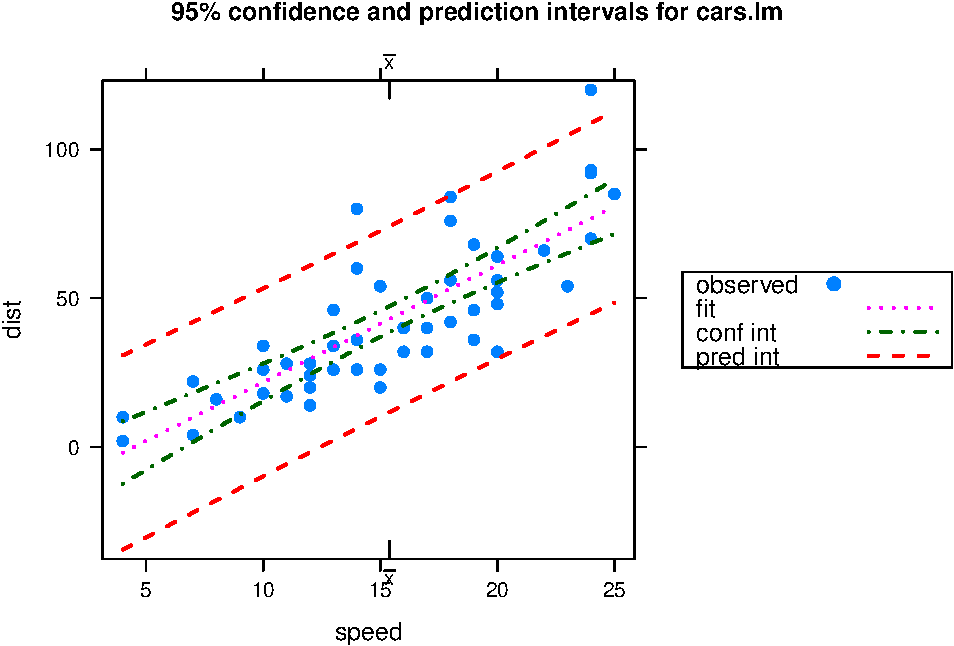
\includegraphics{_main_files/figure-latex/carscipi-1.pdf}
\caption{\label{fig:carscipi}\small A scatterplot with confidence/prediction bands
for the \texttt{cars} data.}
\end{figure}




\section{Model Utility and Inference}\label{sec-model-utility-slr}

\subsection{Hypothesis Tests for the
Parameters}\label{sub-slr-hypoth-test-params}

Much of the attention of SLR is directed toward \(\beta_{1}\) because
when \(\beta_{1}\neq 0\) the mean value of \(Y\) increases (or
decreases) as \(x\) increases. It is really boring when \(\beta_{1}=0\),
because in that case the mean value of \(Y\) remains the same,
regardless of the value of \(x\) (when the regression assumptions hold,
of course). It is thus very important to decide whether or not
\(\beta_{1} = 0\). We address the question with a statistical test of
the null hypothesis \(H_{0}:\beta_{1}=0\) versus the alternative
hypothesis \(H_{1}:\beta_{1}\neq0\), and to do that we need to know the
sampling distribution of \(b_{1}\) when the null hypothesis is true.

To this end we already know from Section
\ref{sub-slr-interval-est-params} that the quantity

\begin{equation} 
T=\frac{b_{1}-\beta_{1}}{S_{b_{1}}}
\end{equation}

has a \(\mathsf{t}(\mathtt{df}=n-2)\) distribution; therefore, when
\(\beta_{1}=0\) the quantity \(b_{1}/S_{b_{1}}\) has a
\(\mathsf{t}(\mathtt{df}=n-2)\) distribution and we can compute a
\(p\)-value by comparing the observed value of \(b_{1}/S{}_{b_{1}}\)
with values under a \(\mathsf{t}(\mathtt{df}=n-2)\) curve.

Similarly, we may test the hypothesis \(H_{0}:\beta_{0}=0\) versus the
alternative \(H_{1}:\beta_{0}\neq0\) with the statistic
\(T=b_{0}/S_{b_{0}}\), where \(S_{b_{0}}\) is given in Section
\ref{sub-slr-interval-est-params}. The test is conducted the same way as
for \(\beta_{1}\).

\subsubsection{How to do it with R}\label{how-to-do-it-with-r-29}

Let us take another look at the output from \texttt{summary(cars.lm)}:

\begin{Shaded}
\begin{Highlighting}[]
\KeywordTok{summary}\NormalTok{(cars.lm)}
\end{Highlighting}
\end{Shaded}

\begin{verbatim}

Call:
lm(formula = dist ~ speed, data = cars)

Residuals:
    Min      1Q  Median      3Q     Max 
-29.069  -9.525  -2.272   9.215  43.201 

Coefficients:
            Estimate Std. Error t value Pr(>|t|)    
(Intercept) -17.5791     6.7584  -2.601   0.0123 *  
speed         3.9324     0.4155   9.464 1.49e-12 ***
---
Signif. codes:  
0 '***' 0.001 '**' 0.01 '*' 0.05 '.' 0.1 ' ' 1

Residual standard error: 15.38 on 48 degrees of freedom
Multiple R-squared:  0.6511,    Adjusted R-squared:  0.6438 
F-statistic: 89.57 on 1 and 48 DF,  p-value: 1.49e-12
\end{verbatim}

In the \texttt{Coefficients} section we find the \(t\) statistics and
the \(p\)-values associated with the tests that the respective
parameters are zero in the fourth and fifth columns. Since the
\(p\)-values are (much) less than 0.05, we conclude that there is strong
evidence that the parameters \(\beta_{1}\neq0\) and \(\beta_{0}\neq0\),
and as such, we say that there is a statistically significant linear
relationship between \texttt{dist} and \texttt{speed}.

\subsection{Simple Coefficient of
Determination}\label{simple-coefficient-of-determination}

It would be nice to have a single number that indicates how well our
linear regression model is doing, and the \emph{simple coefficient of
determination} is designed for that purpose. In what follows, we observe
the values \(Y_{1}\), \(Y_{2}\), \ldots{},\(Y_{n}\), and the goal is to
estimate \(\mu(x_{0})\), the mean value of \(Y\) at the location
\(x_{0}\).

If we disregard the dependence of \(Y\) and \(x\) and base our estimate
only on the \(Y\) values then a reasonable choice for an estimator is
just the MLE of \(\mu\), which is \(\overline{Y}\). Then the errors
incurred by the estimate are just \(Y_{i}-\overline{Y}\) and the
variation about the estimate as measured by the sample variance is
proportional to

\begin{equation}
SSTO=\sum_{i=1}^{n}(Y_{i}-\overline{Y})^{2}.
\end{equation}

The acronym \(SSTO\) stands for \emph{total sum of squares}. And we have
additional information, namely, we have values \(x_{i}\) associated with
each value of \(Y_{i}\). We have seen that this information leads us to
the estimate \(\hat{Y_{i}}\) and the errors incurred are just the
residuals, \(E_{i}=Y_{i}-\hat{Y_{i}}\). The variation associated with
these errors can be measured with

\begin{equation}
SSE=\sum_{i=1}^{n}(Y_{i}-\hat{Y_{i}})^{2}.
\end{equation}

We have seen the \(SSE\) before, which stands for the \emph{sum of
squared errors} or \emph{error sum of squares}. Of course, we would
expect the error to be less in the latter case, since we have used more
information. The improvement in our estimation as a result of the linear
regression model can be measured with the difference \[
(Y_{i}-\overline{Y})-(Y_{i}-\hat{Y_{i}})=\hat{Y_{i}}-\overline{Y}, \]
and we measure the variation in these errors with

\begin{equation}
SSR=\sum_{i=1}^{n}(\hat{Y_{i}}-\overline{Y})^{2},
\end{equation}

also known as the \emph{regression sum of squares}. It is not obvious,
but some algebra proved a famous result known as the \emph{ANOVA
Equality}:

\begin{equation}
\label{eq-anovaeq}
\sum_{i=1}^{n}(Y_{i}-\overline{Y})^{2}=\sum_{i=1}^{n}(\hat{Y_{i}}-\overline{Y})^{2}+\sum_{i=1}^{n}(Y_{i}-\hat{Y_{i}})^{2}
\end{equation}

or in other words,

\begin{equation}
SSTO=SSR+SSE.
\end{equation}

This equality has a nice interpretation. Consider \(SSTO\) to be the
\emph{total variation} of the errors. Think of a decomposition of the
total variation into pieces: one piece measuring the reduction of error
from using the linear regression model, or \emph{explained variation}
(\(SSR\)), while the other represents what is left over, that is, the
errors that the linear regression model doesn't explain, or
\emph{unexplained variation} (\(SSE\)). In this way we see that the
ANOVA equality merely partitions the variation into \[ \mbox{total
variation}=\mbox{explained variation}+\mbox{unexplained variation}.
\] For a single number to summarize how well our model is doing we use
the \emph{simple coefficient of determination} \(r^{2}\), defined by

\begin{equation}
r^{2}=1-\frac{SSE}{SSTO}.
\end{equation}

We interpret \(r^{2}\) as the proportion of total variation that is
explained by the simple linear regression model. When \(r^{2}\) is
large, the model is doing a good job; when \(r^{2}\) is small, the model
is not doing a good job.

Related to the simple coefficient of determination is the sample
correlation coefficient, \(r\). As you can guess, the way we get \(r\)
is by the formula \(|r|=\sqrt{r^{2}}\). The sign of \(r\) is equal the
sign of the slope estimate \(b_{1}\). That is, if the regression line
\(\hat{\mu}(x)\) has positive slope, then \(r=\sqrt{r^{2}}\). Likewise,
if the slope of \(\hat{\mu}(x)\) is negative, then \(r=-\sqrt{r^{2}}\).

\subsubsection{How to do it with R}\label{how-to-do-it-with-r-30}

The primary method to display partitioned sums of squared errors is with
an \emph{ANOVA table}. The command in R to produce such a table is
\texttt{anova}. The input to \texttt{anova} is the result of an
\texttt{lm} call which for the \texttt{cars} data is \texttt{cars.lm}.

\begin{Shaded}
\begin{Highlighting}[]
\KeywordTok{anova}\NormalTok{(cars.lm)}
\end{Highlighting}
\end{Shaded}

\begin{verbatim}
Analysis of Variance Table

Response: dist
          Df Sum Sq Mean Sq F value   Pr(>F)    
speed      1  21186 21185.5  89.567 1.49e-12 ***
Residuals 48  11354   236.5                     
---
Signif. codes:  
0 '***' 0.001 '**' 0.01 '*' 0.05 '.' 0.1 ' ' 1
\end{verbatim}

The output gives \[
r^{2}=1-\frac{SSE}{SSR+SSE}=1-\frac{11353.5}{21185.5+11353.5}\approx0.65.
\]

The interpretation should be: ``The linear regression line accounts for
approximately 65\% of the variation of \texttt{dist} as explained by
\texttt{speed}''.

The value of \(r^{2}\) is stored in the \texttt{r.squared} component of
\texttt{summary(cars.lm)}, which we called \texttt{carsumry}.

\begin{Shaded}
\begin{Highlighting}[]
\NormalTok{carsumry$r.squared}
\end{Highlighting}
\end{Shaded}

\begin{verbatim}
[1] 0.6510794
\end{verbatim}

We already knew this. We saw it in the next to the last line of the
\texttt{summary(cars.lm)} output where it was called
\texttt{Multiple\ R-squared}. Listed right beside it is the
\texttt{Adjusted\ R-squared} which we will discuss in Chapter
\ref{cha-multiple-linear-regression}. For the \texttt{cars} data, we
find \(r\) to be

\begin{Shaded}
\begin{Highlighting}[]
\KeywordTok{sqrt}\NormalTok{(carsumry$r.squared)}
\end{Highlighting}
\end{Shaded}

\begin{verbatim}
[1] 0.8068949
\end{verbatim}

We choose the principal square root because the slope of the regression
line is positive.

\subsection{Overall F statistic}\label{sub-slr-overall-f-statistic}

There is another way to test the significance of the linear regression
model. In SLR, the new way also tests the hypothesis
\(H_{0}:\beta_{1}=0\) versus \(H_{1}:\beta_{1}\neq0\), but it is done
with a new test statistic called the \emph{overall F statistic}. It is
defined by

\begin{equation}
\label{eq-slr-overall-F-statistic}
F=\frac{SSR}{SSE/(n-2)}.
\end{equation}

Under the regression assumptions and when \(H_{0}\) is true, the \(F\)
statistic has an \(\mathtt{f}(\mathtt{df1}=1,\,\mathtt{df2}=n-2)\)
distribution. We reject \(H_{0}\) when \(F\) is large -- that is, when
the explained variation is large relative to the unexplained variation.

All this being said, we have not yet gained much from the overall \(F\)
statistic because we already knew from Section
\ref{sub-slr-hypoth-test-params} how to test
\(H_{0}:\beta_{1} = 0\)\ldots{} we use the Student's \(t\) statistic.
What is worse is that (in the simple linear regression model) it can be
proved that the \(F\) in Equation \eqref{eq-slr-overall-F-statistic} is
exactly the Student's \(t\) statistic for \(\beta_{1}\) squared,

\begin{equation}
F=\left(\frac{b_{1}}{S_{b_{1}}}\right)^{2}.
\end{equation}

So why bother to define the \(F\) statistic? Why not just square the
\(t\) statistic and be done with it? The answer is that the \(F\)
statistic has a more complicated interpretation and plays a more
important role in the multiple linear regression model which we will
study in Chapter \ref{cha-multiple-linear-regression}. See Section
\ref{sub-mlr-overall-f-test} for details.

\subsubsection{How to do it with R}\label{how-to-do-it-with-r-31}

The overall \(F\) statistic and \(p\)-value are displayed in the bottom
line of the \texttt{summary(cars.lm)} output. It is also shown in the
final columns of \texttt{anova(cars.lm)}:

\begin{Shaded}
\begin{Highlighting}[]
\KeywordTok{anova}\NormalTok{(cars.lm)}
\end{Highlighting}
\end{Shaded}

\begin{verbatim}
Analysis of Variance Table

Response: dist
          Df Sum Sq Mean Sq F value   Pr(>F)    
speed      1  21186 21185.5  89.567 1.49e-12 ***
Residuals 48  11354   236.5                     
---
Signif. codes:  
0 '***' 0.001 '**' 0.01 '*' 0.05 '.' 0.1 ' ' 1
\end{verbatim}

Here we see that the \(F\) statistic is 89.57 with a \(p\)-value very
close to zero. The conclusion: there is very strong evidence that
\(H_{0}:\beta_{1} = 0\) is false, that is, there is strong evidence that
\(\beta_{1} \neq 0\). Moreover, we conclude that the regression
relationship between \texttt{dist} and \texttt{speed} is significant.

Note that the value of the \(F\) statistic is the same as the Student's
\(t\) statistic for \texttt{speed} squared.

\section{Residual Analysis}\label{sec-residual-analysis-slr}

We know from our model that \(Y=\mu(x)+\epsilon\), or in other words,
\(\epsilon=Y-\mu(x)\). Further, we know that
\(\epsilon\sim\mathsf{norm}(\mathtt{mean}=0,\,\mathtt{sd}=\sigma)\). We
may estimate \(\epsilon_{i}\) with the \emph{residual}
\(E_{i}=Y_{i}-\hat{Y_{i}}\), where \(\hat{Y_{i}}=\hat{\mu}(x_{i})\). If
the regression assumptions hold, then the residuals should be normally
distributed. We check this in Section \ref{sub-normality-assumption}.
Further, the residuals should have mean zero with constant variance
\(\sigma^{2}\), and we check this in Section
\ref{sub-constant-variance-assumption}. Last, the residuals should be
independent, and we check this in Section
\ref{sub-independence-assumption}.

In every case, we will begin by looking at residual plots -- that is,
scatterplots of the residuals \(E_{i}\) versus index or predicted values
\(\hat{Y_{i}}\) -- and follow up with hypothesis tests.

\subsection{Normality Assumption}\label{sub-normality-assumption}

We can assess the normality of the residuals with graphical methods and
hypothesis tests. To check graphically whether the residuals are
normally distributed we may look at histograms or \emph{q-q} plots. We
first examine a histogram in Figure \ref{fig:normal-hist-cars}, which
was produced by the following code.

\begin{Shaded}
\begin{Highlighting}[]
\KeywordTok{hist}\NormalTok{(}\KeywordTok{residuals}\NormalTok{(cars.lm))}
\end{Highlighting}
\end{Shaded}

\begin{figure}[htbp]
\centering
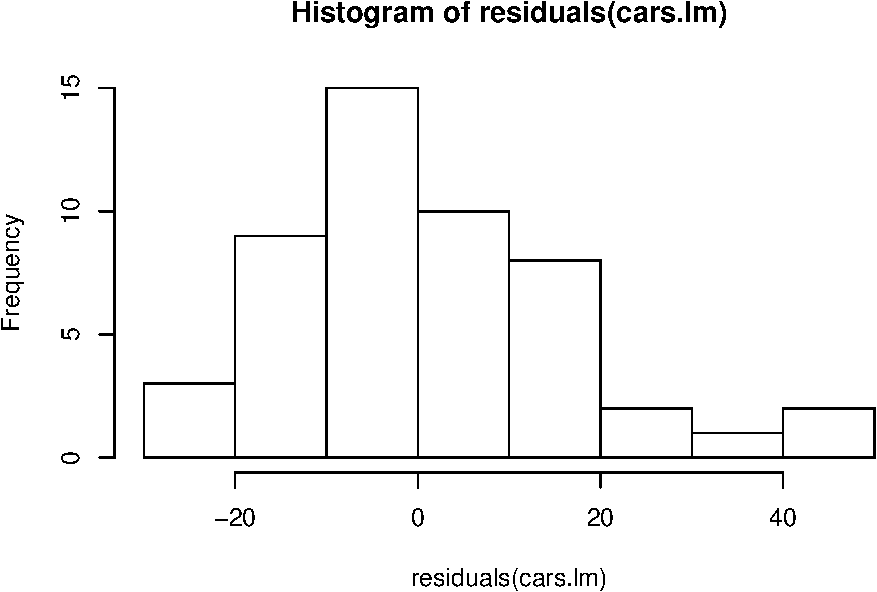
\includegraphics{_main_files/figure-latex/normal-hist-cars-1.pdf}
\caption{\label{fig:normal-hist-cars}\small A histogram of the residuals from the
linear regression model for the \texttt{cars} data. Used for checking
the normality assumption. Look out for any skewness or extreme values;
hopefully the graph is mound shaped and symmetric about zero, with no
outliers.}
\end{figure}







There we see that the distribution of the residuals appears to be mound
shaped, for the most part. We can plot the order statistics of the
studentized residuals versus quantiles from a
\(\mathsf{t}(\mathtt{mean}=0,\,\mathtt{sd}=1)\) distribution with the
command \texttt{qqPlot(cars.lm)} from the \texttt{RcmdrMisc} package
\autocite{RcmdrMisc}, and the results are in Figure
\ref{fig:normal-q-q-plot-cars}. If the assumption of normality were
true, then we would expect points randomly scattered about the dotted
straight line displayed in the figure. In this case, we see a slight
departure from normality in that the dots show a bit of clustering on
one side or the other of the line. The points on the upper end of the
plot also begin to stray from the line. We would say there is some
evidence that the residuals are not perfectly normal.

\begin{Shaded}
\begin{Highlighting}[]
\KeywordTok{library}\NormalTok{(RcmdrMisc)}
\KeywordTok{qqPlot}\NormalTok{(cars.lm)}
\end{Highlighting}
\end{Shaded}

\begin{figure}[htbp]
\centering
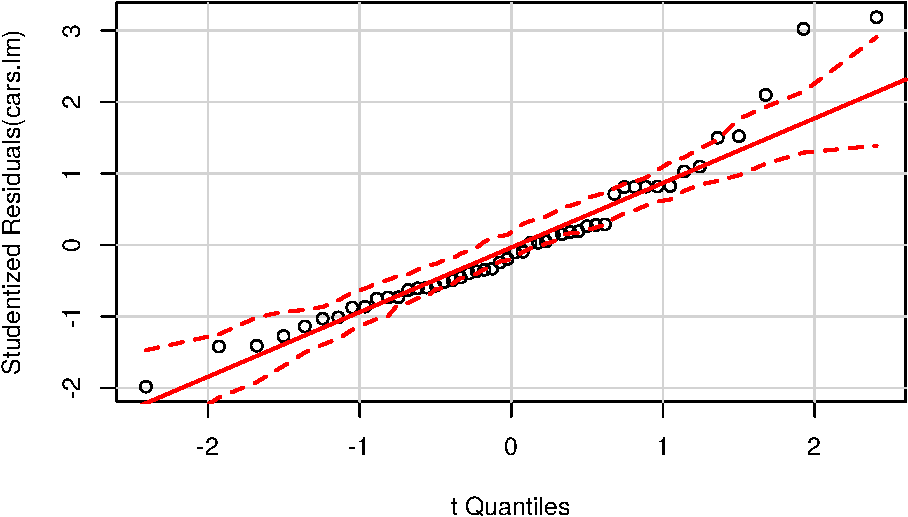
\includegraphics{_main_files/figure-latex/normal-q-q-plot-cars-1.pdf}
\caption{\label{fig:normal-q-q-plot-cars}\small A quantile-quantile plot of the
studentized residuals from the linear regression model for the
\texttt{cars} data. Used for checking the normality assumption. Look out
for any curvature or substantial departures from the straight line;
hopefully the dots hug the line closely and stay within the bands.}
\end{figure}







\subsubsection{Testing the Normality
Assumption}\label{testing-the-normality-assumption}

Even though we may be concerned about the plots, we can use tests to
determine if the evidence present is statistically significant, or if it
could have happened merely by chance. There are many statistical tests
of normality. We will use the Shapiro-Wilk test, since it is known to be
a good test and to be quite powerful. However, there are many other fine
tests of normality including the Anderson-Darling test and the Lillefors
test, just to mention two of them.

The Shapiro-Wilk test is based on the statistic

\begin{equation}
W=\frac{\left(\sum_{i=1}^{n}a_{i}E_{(i)}\right)^{2}}{\sum_{j=1}^{n}E_{j}^{2}},
\end{equation}

where the \(E_{(i)}\) are the ordered residuals and the \(a_{i}\) are
constants derived from the order statistics of a sample of size \(n\)
from a normal distribution. See Section
\ref{sub-shapiro-wilk-normality-test}. We perform the Shapiro-Wilk test
below, using the \texttt{shapiro.test} function from the \texttt{stats}
package \autocite{stats}. The hypotheses are \[
H_{0}:\mbox{ the residuals are normally distributed } \] versus \[
H_{1}:\mbox{ the residuals are not normally distributed.}  \] The
results from R are

\begin{Shaded}
\begin{Highlighting}[]
\KeywordTok{shapiro.test}\NormalTok{(}\KeywordTok{residuals}\NormalTok{(cars.lm))}
\end{Highlighting}
\end{Shaded}

\begin{verbatim}

    Shapiro-Wilk normality test

data:  residuals(cars.lm)
W = 0.94509, p-value = 0.02152
\end{verbatim}

For these data we would reject the assumption of normality of the
residuals at the \(\alpha=0.05\) significance level, but do not lose
heart, because the regression model is reasonably robust to departures
from the normality assumption. As long as the residual distribution is
not highly skewed, then the regression estimators will perform
reasonably well. Moreover, departures from constant variance and
independence will sometimes affect the quantile plots and histograms,
therefore it is wise to delay final decisions regarding normality until
all diagnostic measures have been investigated.

\subsection{Constant Variance
Assumption}\label{sub-constant-variance-assumption}

We will again go to residual plots to try and determine if the spread of
the residuals is changing over time (or index). However, it is
unfortunately not that easy because the residuals do not have constant
variance! In fact, it can be shown that the variance of the residual
\(E_{i}\) is

\begin{equation}
\mbox{Var$(E_{i})$}=\sigma^{2}(1-h_{ii}),\quad i=1,2,\ldots,n,
\end{equation}

where \(h_{ii}\) is a quantity called the \emph{leverage} which is
defined below. Consequently, in order to check the constant variance
assumption we must standardize the residuals before plotting. We
estimate the standard error of \(E_{i}\) with
\(s_{E_{i}}=s\sqrt{(1-h_{ii})}\) and define the \emph{standardized
residuals} \(R_{i}\), \(i=1,2,\ldots,n\), by

\begin{equation} 
R_{i}=\frac{E_{i}}{s\,\sqrt{1-h_{ii}}},\quad i=1,2,\ldots,n.
\end{equation}

For the constant variance assumption we do not need the sign of the
residual so we will plot \(\sqrt{|R_{i}|}\) versus the fitted values. As
we look at a scatterplot of \(\sqrt{|R_{i}|}\) versus \(\hat{Y}_{i}\) we
would expect under the regression assumptions to see a constant band of
observations, indicating no change in the magnitude of the observed
distance from the line. We want to watch out for a fanning-out of the
residuals, or a less common funneling-in of the residuals. Both patterns
indicate a change in the residual variance and a consequent departure
from the regression assumptions, the first an increase, the second a
decrease.

In this case, we plot the standardized residuals versus the fitted
values. The graph may be seen in Figure
\ref{fig:std-resids-fitted-cars}. For these data there does appear to be
somewhat of a slight fanning-out of the residuals.

\begin{Shaded}
\begin{Highlighting}[]
\KeywordTok{plot}\NormalTok{(cars.lm, }\DataTypeTok{which =} \DecValTok{3}\NormalTok{)}
\end{Highlighting}
\end{Shaded}

\begin{figure}[htbp]
\centering
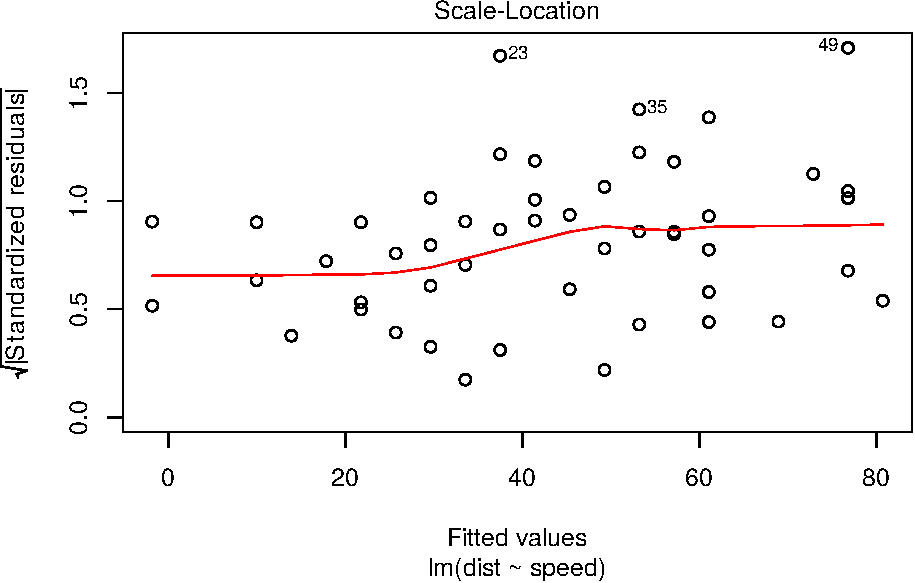
\includegraphics{_main_files/figure-latex/std-resids-fitted-cars-1.pdf}
\caption{\label{fig:std-resids-fitted-cars}\small Plot of standardized residuals
against the fitted values for the \texttt{cars} data. Used for checking
the constant variance assumption. Watch out for any fanning out (or in)
of the dots; hopefully they fall in a constant band.}
\end{figure}






\subsubsection{Testing the Constant Variance
Assumption}\label{testing-the-constant-variance-assumption}

We will use the Breusch-Pagan test to decide whether the variance of the
residuals is nonconstant. The null hypothesis is that the variance is
the same for all observations, and the alternative hypothesis is that
the variance is not the same for all observations. The test statistic is
found by fitting a linear model to the centered squared residuals,

\begin{equation}
W_{i} = E_{i}^{2} - \frac{SSE}{n}, \quad i=1,2,\ldots,n.
\end{equation}

By default the same explanatory variables are used in the new model
which produces fitted values \(\hat{W}_{i}\), \(i=1,2,\ldots,n\). The
Breusch-Pagan test statistic in R is then calculated with

\begin{equation}
BP=n\sum_{i=1}^{n}\hat{W}_{i}^{2}\div\sum_{i=1}^{n}W_{i}^{2}.
\end{equation}

We reject the null hypothesis if \(BP\) is too large, which happens when
the explained variation i the new model is large relative to the
unexplained variation in the original model. We do it in R with the
\texttt{bptest} function from the \texttt{lmtest} package
\autocite{lmtest}.

\begin{Shaded}
\begin{Highlighting}[]
\KeywordTok{bptest}\NormalTok{(cars.lm)}
\end{Highlighting}
\end{Shaded}

\begin{verbatim}

    studentized Breusch-Pagan test

data:  cars.lm
BP = 3.2149, df = 1, p-value = 0.07297
\end{verbatim}

For these data we would not reject the null hypothesis at the
\(\alpha=0.05\) level. There is relatively weak evidence against the
assumption of constant variance.

\subsection{Independence Assumption}\label{sub-independence-assumption}

One of the strongest of the regression assumptions is the one regarding
independence. Departures from the independence assumption are often
exhibited by correlation (or autocorrelation, literally,
self-correlation) present in the residuals. There can be positive or
negative correlation.

Positive correlation is displayed by positive residuals followed by
positive residuals, and negative residuals followed by negative
residuals. Looking from left to right, this is exhibited by a cyclical
feature in the residual plots, with long sequences of positive residuals
being followed by long sequences of negative ones.

On the other hand, negative correlation implies positive residuals
followed by negative residuals, which are then followed by positive
residuals, \emph{etc}. Consequently, negatively correlated residuals are
often associated with an alternating pattern in the residual plots. We
examine the residual plot in Figure \ref{fig:resids-fitted-cars}. There
is no obvious cyclical wave pattern or structure to the residual plot.

\begin{Shaded}
\begin{Highlighting}[]
\KeywordTok{plot}\NormalTok{(cars.lm, }\DataTypeTok{which =} \DecValTok{1}\NormalTok{)}
\end{Highlighting}
\end{Shaded}

\begin{figure}[htbp]
\centering
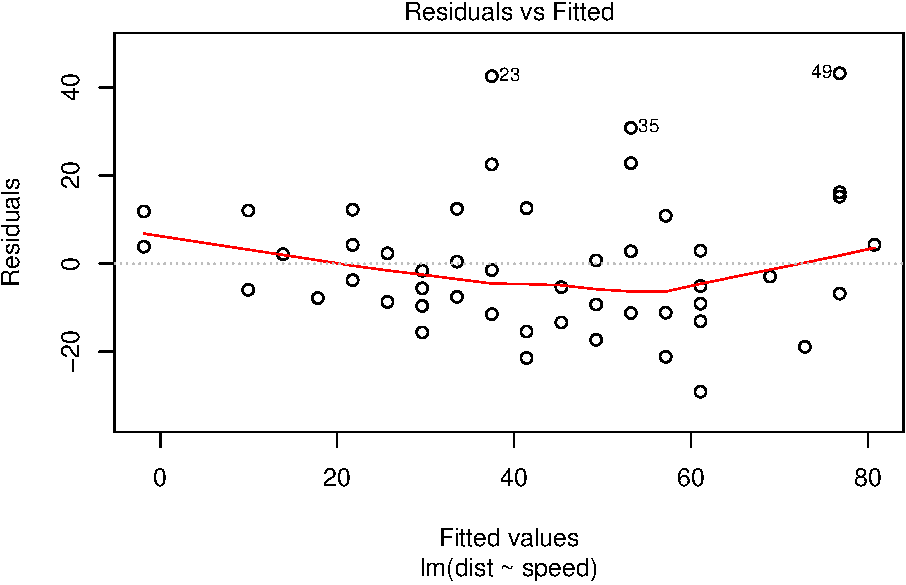
\includegraphics{_main_files/figure-latex/resids-fitted-cars-1.pdf}
\caption{\label{fig:resids-fitted-cars}\small Plot of the residuals versus the
fitted values for the \texttt{cars} data. Used for checking the
independence assumption. Watch out for any patterns or structure;
hopefully the points are randomly scattered on the plot.}
\end{figure}






\subsubsection{Testing the Independence
Assumption}\label{testing-the-independence-assumption}

We may statistically test whether there is evidence of autocorrelation
in the residuals with the Durbin-Watson test. The test is based on the
statistic

\begin{equation}
D=\frac{\sum_{i=2}^{n}(E_{i}-E_{i-1})^{2}}{\sum_{j=1}^{n}E_{j}^{2}}.
\end{equation}

Exact critical values are difficult to obtain, but R will calculate the
\emph{p}-value to great accuracy. It is performed with the
\texttt{dwtest} function from the \texttt{lmtest} package
\autocite{lmtest}. We will conduct a two sided test that the correlation
is not zero, which is not the default (the default is to test that the
autocorrelation is positive).

\begin{Shaded}
\begin{Highlighting}[]
\KeywordTok{dwtest}\NormalTok{(cars.lm, }\DataTypeTok{alternative =} \StringTok{"two.sided"}\NormalTok{)}
\end{Highlighting}
\end{Shaded}

\begin{verbatim}

    Durbin-Watson test

data:  cars.lm
DW = 1.6762, p-value = 0.1904
alternative hypothesis: true autocorrelation is not 0
\end{verbatim}

In this case we do not reject the null hypothesis at the \(\alpha=0.05\)
significance level; there is very little evidence of nonzero
autocorrelation in the residuals.

\subsection{Remedial Measures}\label{remedial-measures}

We often find problems with our model that suggest that at least one of
the three regression assumptions is violated. What do we do then? There
are many measures at the statistician's disposal, and we mention
specific steps one can take to improve the model under certain types of
violation.

\begin{itemize}
\tightlist
\item
  \textbf{Mean response is not linear} We can directly modify the model
  to better approximate the mean response. In particular, perhaps a
  polynomial regression function of the form \[ \mu(x) =
   \beta_{0} + \beta_{1}x_{1} + \beta_{2}x_{1}^{2} \] would be
  appropriate. Alternatively, we could have a function of the form
  \[ \mu(x)=\beta_{0}\mathrm{e}^{\beta_{1}x}.  \] Models like these are
  studied in nonlinear regression courses.
\item
  \textbf{Error variance is not constant} Sometimes a transformation of
  the dependent variable will take care of the problem. There is a large
  class of them called \emph{Box-Cox transformations}. They take the
  form

  \begin{equation}
   Y^{\ast}=Y^{\lambda},
   \end{equation}

  where \(\lambda\) is a constant. (The method proposed by Box and Cox
  will determine a suitable value of \(\lambda\) automatically by
  maximum likelihood). The class contains the transformations

  \begin{alignat*}{1} \lambda=2,\quad &
   Y^{\ast}=Y^{2}\\ \lambda=0.5,\quad &
   Y^{\ast}=\sqrt{Y}\\ \lambda=0,\quad & Y^{\ast}=\ln\:
   Y\\ \lambda=-1,\quad & Y^{\ast}= 1/Y \end{alignat*}

  Alternatively, we can use the method of \emph{weighted least squares}.
  This is studied in more detail in later classes.
\item
  \textbf{Error distribution is not normal} The same transformations for
  stabilizing the variance are equally appropriate for smoothing the
  residuals to a more Gaussian form. In fact, often we will kill two
  birds with one stone.
\item
  \textbf{Errors are not independent} There is a large class of
  autoregressive models to be used in this situation which occupy the
  latter part of Chapter \ref{cha-time-series}.
\end{itemize}

\section{Other Diagnostic Tools}\label{sec-other-diagnostic-tools-slr}

There are two types of observations with which we must be especially
careful:

\begin{itemize}
\tightlist
\item
  \textbf{Influential observations} are those that have a substantial
  effect on our estimates, predictions, or inferences. A small change in
  an influential observation is followed by a large change in the
  parameter estimates or inferences.
\item
  \textbf{Outlying observations} are those that fall fall far from the
  rest of the data. They may be indicating a lack of fit for our
  regression model, or they may just be a mistake or typographical error
  that should be corrected. Regardless, special attention should be
  given to these observations. An outlying observation may or may not be
  influential.
\end{itemize}

We will discuss outliers first because the notation builds sequentially
in that order.

\subsection{Outliers}\label{outliers}

There are three ways that an observation \((x_{i},y_{i})\) might be
identified as an outlier: it can have an \(x_{i}\) value which falls far
from the other \(x\) values, it can have a \(y_{i}\) value which falls
far from the other \(y\) values, or it can have both its \(x_{i}\) and
\(y_{i}\) values falling far from the other \(x\) and \(y\) values.

\subsection{Leverage}\label{leverage}

Leverage statistics are designed to identify observations which have
\(x\) values that are far away from the rest of the data. In the simple
linear regression model the leverage of \(x_{i}\) is denoted by
\(h_{ii}\) and defined by

\begin{equation}
h_{ii}=\frac{1}{n}+\frac{(x_{i}-\overline{x})^{2}}{\sum_{k=1}^{n}(x_{k}-\overline{x})^{2}},\quad i=1,2,\ldots,n.
\end{equation}

The formula has a nice interpretation in the SLR model: if the distance
from \(x_{i}\) to \(\overline{x}\) is large relative to the other
\(x\)'s then \(h_{ii}\) will be close to 1.

Leverages have nice mathematical properties; for example, they satisfy

\begin{equation}
\label{eq-slr-leverage-between}
0\leq h_{ii}\leq1,
\end{equation}

and their sum is

\begin{eqnarray}
\label{eq-slr-average-leverage}
\sum_{i=1}^{n}h_{ii} & = & \sum_{i=1}^{n}\left[\frac{1}{n}+\frac{(x_{i}-\overline{x})^{2}}{\sum_{k=1}^{n}(x_{k}-\overline{x})^{2}}\right],\\
 & = & \frac{n}{n}+\frac{\sum_{i}(x_{i}-\overline{x})^{2}}{\sum_{k}(x_{k}-\overline{x})^{2}},\\
 & = & 2.
\end{eqnarray}

A rule of thumb is to consider leverage values to be large if they are
more than double their average size (which is \(2/n\) according to
Equation \eqref{eq-slr-average-leverage}). So leverages larger than
\(4/n\) are suspect. Another rule of thumb is to say that values bigger
than 0.5 indicate high leverage, while values between 0.3 and 0.5
indicate moderate leverage.

\subsection{Standardized and Studentized Deleted
Residuals}\label{standardized-and-studentized-deleted-residuals}

We have already encountered the \emph{standardized residuals} \(r_{i}\)
in Section \ref{sub-constant-variance-assumption}; they are merely
residuals that have been divided by their respective standard
deviations:

\begin{equation}
R_{i}=\frac{E_{i}}{S\sqrt{1-h_{ii}}},\quad i=1,2,\ldots,n.
\end{equation}

Values of \(|R_{i}| > 2\) are extreme and suggest that the observation
has an outlying \(y\)-value.

Now delete the \(i^{\mathrm{th}}\) case and fit the regression function
to the remaining \(n - 1\) cases, producing a fitted value
\(\hat{Y}_{(i)}\) with \emph{deleted residual}
\(D_{i}=Y_{i}-\hat{Y}_{(i)}\). It is shown in later classes that

\begin{equation}
\mbox{Var $(D_{i})$}=\frac{S_{(i)}^{2}}{1-h_{ii}},\quad i=1,2,\ldots,n,
\end{equation}

so that the \emph{studentized deleted residuals} \(t_{i}\) defined by

\begin{equation}
\label{eq-slr-studentized-deleted-resids}
t_{i}=\frac{D_{i}}{S_{(i)}/(1-h_{ii})},\quad i=1,2,\ldots,n,
\end{equation}

have a \(\mathsf{t}(\mathtt{df}=n-3)\) distribution and we compare
observed values of \(t_{i}\) to this distribution to decide whether or
not an observation is extreme.

The folklore in regression classes is that a test based on the statistic
in Equation \eqref{eq-slr-studentized-deleted-resids} can be too
liberal. A rule of thumb is if we suspect an observation to be an
outlier \emph{before} seeing the data then we say it is significantly
outlying if its two-tailed \(p\)-value is less than \(\alpha\), but if
we suspect an observation to be an outlier \emph{after} seeing the data
then we should only say it is significantly outlying if its two-tailed
\(p\)-value is less than \(\alpha/n\). The latter rule of thumb is
called the \emph{Bonferroni approach} and can be overly conservative for
large data sets. The responsible statistician should look at the data
and use his/her best judgement, in every case.

\subsubsection{How to do it with R}\label{how-to-do-it-with-r-32}

We can calculate the standardized residuals with the \texttt{rstandard}
function. The input is the \texttt{lm} object, which is
\texttt{cars.lm}.

\begin{Shaded}
\begin{Highlighting}[]
\NormalTok{sres <-}\StringTok{ }\KeywordTok{rstandard}\NormalTok{(cars.lm)}
\NormalTok{sres[}\DecValTok{1}\NormalTok{:}\DecValTok{5}\NormalTok{]}
\end{Highlighting}
\end{Shaded}

\begin{verbatim}
         1          2          3          4          5 
 0.2660415  0.8189327 -0.4013462  0.8132663  0.1421624 
\end{verbatim}

We can find out which observations have studentized residuals larger
than two with the command

\begin{Shaded}
\begin{Highlighting}[]
\NormalTok{sres[}\KeywordTok{which}\NormalTok{(}\KeywordTok{abs}\NormalTok{(sres) >}\StringTok{ }\DecValTok{2}\NormalTok{)]}
\end{Highlighting}
\end{Shaded}

\begin{verbatim}
      23       35       49 
2.795166 2.027818 2.919060 
\end{verbatim}

In this case, we see that observations 23, 35, and 49 are potential
outliers with respect to their \(y\)-value. We can compute the
studentized deleted residuals with \texttt{rstudent}:

\begin{Shaded}
\begin{Highlighting}[]
\NormalTok{sdelres <-}\StringTok{ }\KeywordTok{rstudent}\NormalTok{(cars.lm)}
\NormalTok{sdelres[}\DecValTok{1}\NormalTok{:}\DecValTok{5}\NormalTok{]}
\end{Highlighting}
\end{Shaded}

\begin{verbatim}
         1          2          3          4          5 
 0.2634500  0.8160784 -0.3978115  0.8103526  0.1407033 
\end{verbatim}

We should compare these values with critical values from a
\(\mathsf{t}(\mathtt{df}=n-3)\) distribution, which in this case is
\(\mathsf{t}(\mathtt{df}=50-3=47)\). We can calculate a 0.005 quantile
and check with

\begin{Shaded}
\begin{Highlighting}[]
\NormalTok{t0}\FloatTok{.005} \NormalTok{<-}\StringTok{ }\KeywordTok{qt}\NormalTok{(}\FloatTok{0.005}\NormalTok{, }\DataTypeTok{df =} \DecValTok{47}\NormalTok{, }\DataTypeTok{lower.tail =} \OtherTok{FALSE}\NormalTok{)}
\NormalTok{sdelres[}\KeywordTok{which}\NormalTok{(}\KeywordTok{abs}\NormalTok{(sdelres) >}\StringTok{ }\NormalTok{t0}\FloatTok{.005}\NormalTok{)]}
\end{Highlighting}
\end{Shaded}

\begin{verbatim}
      23       49 
3.022829 3.184993 
\end{verbatim}

This means that observations 23 and 49 have a large studentized deleted
residual. The leverages can be found with the \texttt{hatvalues}
function:

\begin{Shaded}
\begin{Highlighting}[]
\NormalTok{leverage <-}\StringTok{ }\KeywordTok{hatvalues}\NormalTok{(cars.lm)}
\NormalTok{leverage[}\KeywordTok{which}\NormalTok{(leverage >}\StringTok{ }\DecValTok{4}\NormalTok{/}\DecValTok{50}\NormalTok{)]}
\end{Highlighting}
\end{Shaded}

\begin{verbatim}
         1          2         50 
0.11486131 0.11486131 0.08727007 
\end{verbatim}

Here we see that observations 1, 2, and 50 have leverages bigger than
double their mean value. These observations would be considered outlying
with respect to their \(x\) value (although they may or may not be
influential).

\subsection{Influential Observations}\label{influential-observations}

\subsubsection{\texorpdfstring{\(DFBETAS\) and
\(DFFITS\)}{DFBETAS and DFFITS}}\label{dfbetas-and-dffits}

Any time we do a statistical analysis, we are confronted with the
variability of data. It is always a concern when an observation plays
too large a role in our regression model, and we would not like or
procedures to be overly influenced by the value of a single observation.
Hence, it becomes desirable to check to see how much our estimates and
predictions would change if one of the observations were not included in
the analysis. If an observation changes the estimates/predictions a
large amount, then the observation is influential and should be
subjected to a higher level of scrutiny.

We measure the change in the parameter estimates as a result of deleting
an observation with \(DFBETAS\). The \(DFBETAS\) for the intercept
\(b_{0}\) are given by

\begin{equation}
(DFBETAS)_{0(i)}=\frac{b_{0}-b_{0(i)}}{S_{(i)}\sqrt{\frac{1}{n}+\frac{\overline{x}^{2}}{\sum_{i=1}^{n}(x_{i}-\overline{x})^{2}}}},\quad i=1,2,\ldots,n.
\end{equation}

and the \(DFBETAS\) for the slope \(b_{1}\) are given by

\begin{equation}
(DFBETAS)_{1(i)}=\frac{b_{1}-b_{1(i)}}{S_{(i)}\left[\sum_{i=1}^{n}(x_{i}-\overline{x})^{2}\right]^{-1/2}},\quad i=1,2,\ldots,n.
\end{equation}

See Section \ref{sec-residual-analysis-mlr} for a better way to write
these. The signs of the \(DFBETAS\) indicate whether the coefficients
would increase or decrease as a result of including the observation. If
the \(DFBETAS\) are large, then the observation has a large impact on
those regression coefficients. We label observations as suspicious if
their \(DFBETAS\) have magnitude greater 1 for small data or
\(2/\sqrt{n}\) for large data sets. We can calculate the \(DFBETAS\)
with the \texttt{dfbetas} function (some output has been omitted):

\begin{Shaded}
\begin{Highlighting}[]
\NormalTok{dfb <-}\StringTok{ }\KeywordTok{dfbetas}\NormalTok{(cars.lm)}
\KeywordTok{head}\NormalTok{(dfb)}
\end{Highlighting}
\end{Shaded}

\begin{verbatim}
  (Intercept)       speed
1  0.09440188 -0.08624563
2  0.29242487 -0.26715961
3 -0.10749794  0.09369281
4  0.21897614 -0.19085472
5  0.03407516 -0.02901384
6 -0.11100703  0.09174024
\end{verbatim}

We see that the inclusion of the first observation slightly increases
the \texttt{Intercept} and slightly decreases the coefficient on
\texttt{speed}.

We can measure the influence that an observation has on its fitted value
with \(DFFITS\). These are calculated by deleting an observation,
refitting the model, recalculating the fit, then standardizing. The
formula is

\begin{equation}
(DFFITS)_{i}=\frac{\hat{Y_{i}}-\hat{Y}_{(i)}}{S_{(i)}\sqrt{h_{ii}}},\quad i=1,2,\ldots,n.
\end{equation}

The value represents the number of standard deviations of
\(\hat{Y_{i}}\) that the fitted value \(\hat{Y_{i}}\) increases or
decreases with the inclusion of the \(i^{\textrm{th}}\) observation. We
can compute them with the \texttt{dffits} function.

\begin{Shaded}
\begin{Highlighting}[]
\NormalTok{dff <-}\StringTok{ }\KeywordTok{dffits}\NormalTok{(cars.lm)}
\NormalTok{dff[}\DecValTok{1}\NormalTok{:}\DecValTok{5}\NormalTok{]}
\end{Highlighting}
\end{Shaded}

\begin{verbatim}
          1           2           3           4           5 
 0.09490289  0.29397684 -0.11039550  0.22487854  0.03553887 
\end{verbatim}

A rule of thumb is to flag observations whose \(DFFIT\) exceeds one in
absolute value, but there are none of those in this data set.

\subsubsection{Cook's Distance}\label{cooks-distance}

The \(DFFITS\) are good for measuring the influence on a single fitted
value, but we may want to measure the influence an observation has on
all of the fitted values simultaneously. The statistics used for
measuring this are Cook's distances which may be calculated\footnote{Rescaling
  the data gets the job done but a better way to avoid the
  multicollinearity introduced by the higher order terms is with
  \emph{orthogonal polynomials}, whose coefficients are chosen just
  right so that the polynomials are not correlated with each other. This
  is beginning to linger outside the scope of this book, however, so we
  will content ourselves with a brief mention and then stick with the
  rescaling approach in the discussion that follows. A nice example of
  orthogonal polynomials in action can be run with
  \texttt{example(cars)}.} by the formula

\begin{equation}
\label{eq-slr-cooks-distance}
D_{i}=\frac{E_{i}^{2}}{(p+1)S^{2}}\cdot\frac{h_{ii}}{(1-h_{ii})^{2}},\quad i=1,2,\ldots,n.
\end{equation}

It shows that Cook's distance depends both on the residual \(E_{i}\) and
the leverage \(h_{ii}\) and in this way \(D_{i}\) contains information
about outlying \(x\) and \(y\) values.

To assess the significance of \(D\), we compare to quantiles of an
\(\mathsf{f}(\mathtt{df1}=2,\,\mathtt{df2}=n-2)\) distribution. A rule
of thumb is to classify observations falling higher than the
\(50^{\mathrm{th}}\) percentile as being extreme.

\subsubsection{How to do it with R}\label{how-to-do-it-with-r-33}

We can calculate the Cook's Distances with the \texttt{cooks.distance}
function.

\begin{Shaded}
\begin{Highlighting}[]
\NormalTok{cooksD <-}\StringTok{ }\KeywordTok{cooks.distance}\NormalTok{(cars.lm)}
\NormalTok{cooksD[}\DecValTok{1}\NormalTok{:}\DecValTok{4}\NormalTok{]}
\end{Highlighting}
\end{Shaded}

\begin{verbatim}
          1           2           3           4 
0.004592312 0.043513991 0.006202350 0.025467338 
\end{verbatim}

We can look at a plot of the Cook's distances with the command
\texttt{plot(cars.lm,\ which\ =\ 4)}.

\begin{Shaded}
\begin{Highlighting}[]
\KeywordTok{plot}\NormalTok{(cars.lm, }\DataTypeTok{which =} \DecValTok{4}\NormalTok{)}
\end{Highlighting}
\end{Shaded}

\begin{figure}[htbp]
\centering
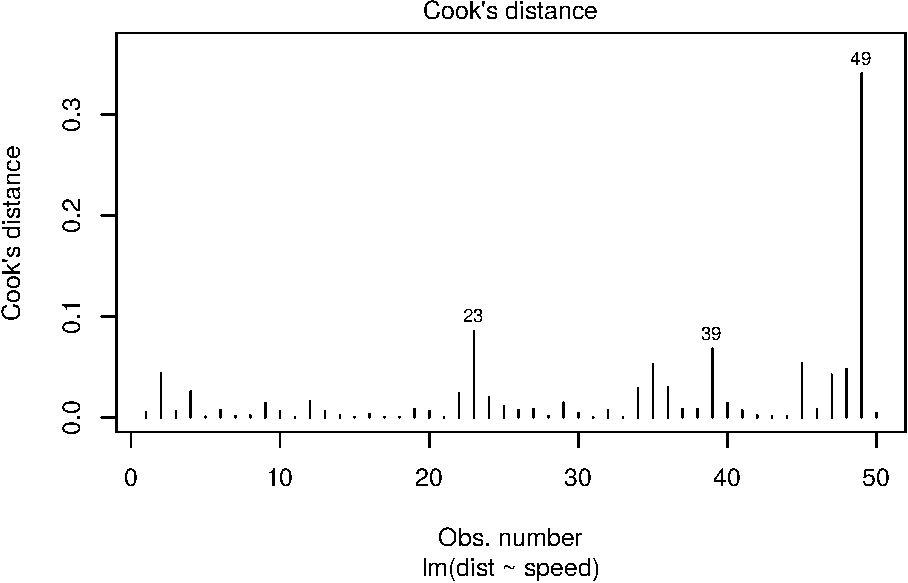
\includegraphics{_main_files/figure-latex/cooks-distance-cars-1.pdf}
\caption{\label{fig:cooks-distance-cars}\small Cook's distances for the
\texttt{cars} data. Used for checking for influential and/our outlying
observations. Values with large Cook's distance merit further
investigation.}
\end{figure}






Observations with the largest Cook's D values are labeled, hence we see
that observations 23, 39, and 49 are suspicious. However, we need to
compare to the quantiles of an
\(\mathsf{f}(\mathtt{df1} = 2, \,\mathtt{df2} = 48)\) distribution:

\begin{Shaded}
\begin{Highlighting}[]
\NormalTok{F0}\FloatTok{.50} \NormalTok{<-}\StringTok{ }\KeywordTok{qf}\NormalTok{(}\FloatTok{0.5}\NormalTok{, }\DataTypeTok{df1 =} \DecValTok{2}\NormalTok{, }\DataTypeTok{df2 =} \DecValTok{48}\NormalTok{)}
\KeywordTok{any}\NormalTok{(cooksD >}\StringTok{ }\NormalTok{F0}\FloatTok{.50}\NormalTok{)}
\end{Highlighting}
\end{Shaded}

\begin{verbatim}
[1] FALSE
\end{verbatim}

We see that with this data set there are no observations with extreme
Cook's distance, after all.

\subsection{All Influence Measures
Simultaneously}\label{all-influence-measures-simultaneously}

We can display the result of diagnostic checking all at once in one
table, with potentially influential points displayed. We do it with the
command \texttt{influence.measures(cars.lm)}:

\begin{Shaded}
\begin{Highlighting}[]
\KeywordTok{influence.measures}\NormalTok{(cars.lm)}
\end{Highlighting}
\end{Shaded}

The output is a huge matrix display, which we have omitted in the
interest of brevity. A point is identified if it is classified to be
influential with respect to any of the diagnostic measures. Here we see
that observations 2, 11, 15, and 18 merit further investigation.

We can also look at all diagnostic plots at once with the commands

\begin{Shaded}
\begin{Highlighting}[]
\KeywordTok{plot}\NormalTok{(cars.lm)}
\end{Highlighting}
\end{Shaded}

The \texttt{par} command is used so that \(2\times 2 = 4\) plots will be
shown on the same display. The diagnostic plots for the \texttt{cars}
data are shown in Figure \ref{fig:diagnostic-plots-cars}.

\begin{Shaded}
\begin{Highlighting}[]
\KeywordTok{par}\NormalTok{(}\DataTypeTok{mfrow =} \KeywordTok{c}\NormalTok{(}\DecValTok{2}\NormalTok{,}\DecValTok{2}\NormalTok{))}
\KeywordTok{plot}\NormalTok{(cars.lm)}
\end{Highlighting}
\end{Shaded}

\begin{figure}[htbp]
\centering
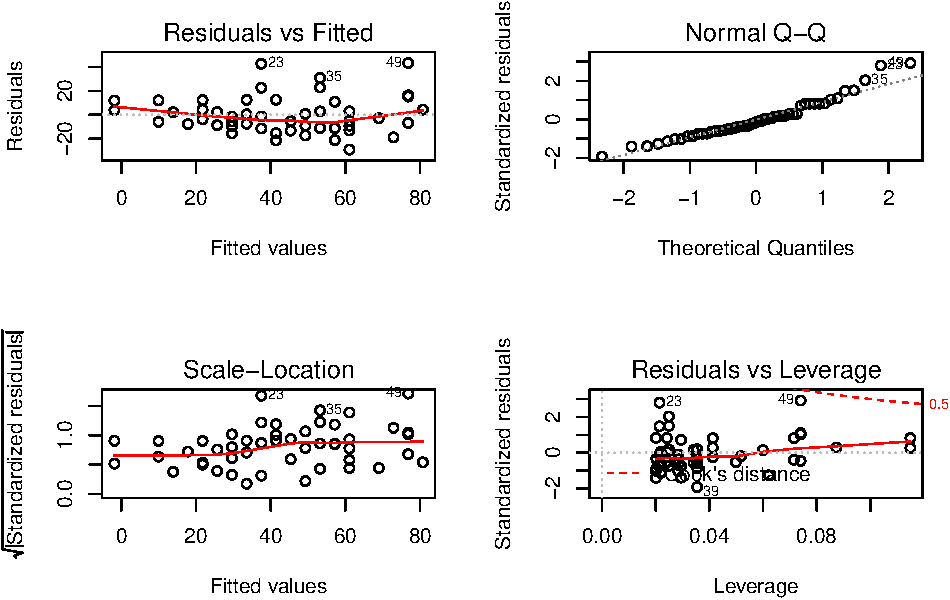
\includegraphics{_main_files/figure-latex/diagnostic-plots-cars-1.pdf}
\caption{\label{fig:diagnostic-plots-cars}\small Diagnostic plots for the
\texttt{cars} data.}
\end{figure}

\begin{Shaded}
\begin{Highlighting}[]
\KeywordTok{par}\NormalTok{(}\DataTypeTok{mfrow =} \KeywordTok{c}\NormalTok{(}\DecValTok{1}\NormalTok{,}\DecValTok{1}\NormalTok{))}
\end{Highlighting}
\end{Shaded}




We have discussed all of the plots except the last, which is possibly
the most interesting. It shows Residuals vs.~Leverage, which will
identify outlying \(y\) values versus outlying \(x\) values. Here we see
that observation 23 has a high residual, but low leverage, and it turns
out that observations 1 and 2 have relatively high leverage but
low/moderate leverage (they are on the right side of the plot, just
above the horizontal line). Observation 49 has a large residual with a
comparatively large leverage.

We can identify the observations with the \texttt{identify} command; it
allows us to display the observation number of dots on the plot. First,
we plot the graph, then we call \texttt{identify}:

\begin{Shaded}
\begin{Highlighting}[]
\KeywordTok{plot}\NormalTok{(cars.lm, }\DataTypeTok{which =} \DecValTok{5}\NormalTok{)          }\CommentTok{# std'd resids vs lev plot}
\KeywordTok{identify}\NormalTok{(leverage, sres, }\DataTypeTok{n =} \DecValTok{4}\NormalTok{)   }\CommentTok{# identify 4 points}
\end{Highlighting}
\end{Shaded}

The graph with the identified points is omitted (but the plain plot is
shown in the bottom right corner of Figure
\ref{fig:diagnostic-plots-cars}). Observations 1 and 2 fall on the far
right side of the plot, near the horizontal axis.

\section{Exercises}\label{exercises-4}

\bigskip

\begin{xca}
Prove the ANOVA equality, Equation \eqref{eq-anovaeq}. \emph{Hint}: show
that \[
\sum_{i=1}^{n}(Y_{i}-\hat{Y_{i}})(\hat{Y_{i}}-\overline{Y})=0.
\]
\end{xca}

\bigskip

\begin{xca}
Solve the following system of equations for \(\beta_{1}\) and
\(\beta_{0}\) to find the MLEs for slope and intercept in the simple
linear regression model.

\begin{eqnarray*}
n\beta_{0}+\beta_{1}\sum_{i=1}^{n}x_{i} & = & \sum_{i=1}^{n}y_{i}\\
\beta_{0}\sum_{i=1}^{n}x_{i}+\beta_{1}\sum_{i=1}^{n}x_{i}^{2} & = & \sum_{i=1}^{n}x_{i}y_{i}
\end{eqnarray*}
\end{xca}

\bigskip

\begin{xca}
Show that the formula given in Equation
\eqref{eq-sample-correlation-formula} is equivalent to \[
\hat{\beta}_{1} =
\frac{\sum_{i=1}^{n}x_{i}y_{i}-\left.\left(\sum_{i=1}^{n}x_{i}\right)\left(\sum_{i=1}^{n}y_{i}\right)\right/
n}{\sum_{i=1}^{n}x_{i}^{2}-\left.\left(\sum_{i=1}^{n}x_{i}\right)^{2}\right/
n}.  \]
\end{xca}

\chapter{Multiple Linear
Regression}\label{cha-multiple-linear-regressionl}

We know a lot about simple linear regression models, and a next step is
to study multiple regression models that have more than one independent
(explanatory) variable. In the discussion that follows we will assume
that we have \(p\) explanatory variables, where \(p > 1\).

The language is phrased in matrix terms -- for two reasons. First, it is
quicker to write and (arguably) more pleasant to read. Second, the
matrix approach will be required for later study of the subject; the
reader might as well be introduced to it now.

Most of the results are stated without proof or with only a cursory
justification. Those yearning for more should consult an advanced text
in linear regression for details, such as \emph{Applied Linear
Regression Models} \autocite{Neter1996} or \emph{Linear Models: Least
Squares and Alternatives} \autocite{Rao1999}.

\textbf{What do I want them to know?}

\begin{itemize}
\tightlist
\item
  the basic MLR model, and how it relates to the SLR
\item
  how to estimate the parameters and use those estimates to make
  predictions
\item
  basic strategies to determine whether or not the model is doing a good
  job
\item
  a few thoughts about selected applications of the MLR, such as
  polynomial, interaction, and dummy variable models
\item
  some of the uses of residuals to diagnose problems
\item
  hints about what will be coming later
\end{itemize}

\section{The Multiple Linear Regression Model}\label{sec-the-mlr-model}

The first thing to do is get some better notation. We will write

\begin{equation}
\mathbf{Y}_{\mathrm{n}\times1}=
\begin{bmatrix}y_{1}\\
y_{2}\\
\vdots\\
y_{n}
\end{bmatrix},
\quad \mbox{and}\quad \mathbf{X}_{\mathrm{n}\times(\mathrm{p}+1)}=
\begin{bmatrix}1 & x_{11} & x_{21} & \cdots & x_{p1}\\
1 & x_{12} & x_{22} & \cdots & x_{p2}\\
\vdots & \vdots & \vdots & \ddots & \vdots\\
1 & x_{1n} & x_{2n} & \cdots & x_{pn}
\end{bmatrix}.
\end{equation}

The vector \(\mathbf{Y}\) is called the \emph{response vector}
\index{response vector} and the matrix \(\mathbf{X}\) is called the
\emph{model matrix} \index{model matrix}. As in Chapter
\ref{cha-simple-linear-regression}, the most general assumption that
relates \(\mathbf{Y}\) to \(\mathbf{X}\) is

\begin{equation}
\mathbf{Y}=\mu(\mathbf{X})+\upepsilon,
\end{equation}

where \(\mu\) is some function (the \emph{signal}) and \(\upepsilon\) is
the \emph{noise} (everything else). We usually impose some structure on
\(\mu\) and \(\upepsilon\). In particular, the standard multiple linear
regression model \index{model!multiple linear regression} assumes

\begin{equation}
\mathbf{Y}=\mathbf{X}\upbeta+\upepsilon,
\end{equation}

where the parameter vector \(\upbeta\) looks like

\begin{equation}
\upbeta_{(\mathrm{p}+1)\times1}=\begin{bmatrix}\beta_{0} & \beta_{1} & \cdots & \beta_{p}\end{bmatrix}^{\mathrm{T}},
\end{equation}

and the random vector
\(\upepsilon_{\mathrm{n}\times1}=\begin{bmatrix}\epsilon_{1} & \epsilon_{2} & \cdots & \epsilon_{n}\end{bmatrix}^{\mathrm{T}}\)
is assumed to be distributed

\begin{equation}
\upepsilon\sim\mathsf{mvnorm}\left(\mathtt{mean}=\mathbf{0}_{\mathrm{n}\times1},\,\mathtt{sigma}=\sigma^{2}\mathbf{I}_{\mathrm{n}\times\mathrm{n}}\right).
\end{equation}

The assumption on \(\upepsilon\) is equivalent to the assumption that
\(\epsilon_{1}\), \(\epsilon_{2}\), \ldots{}, \(\epsilon_{n}\) are IID
\(\mathsf{norm}(\mathtt{mean}=0,\,\mathtt{sd}=\sigma)\). It is a linear
model because the quantity \(\mu(\mathbf{X})=\mathbf{X}\upbeta\) is
linear in the parameters \(\beta_{0}\), \(\beta_{1}\), \ldots{},
\(\beta_{p}\). It may be helpful to see the model in expanded form; the
above matrix formulation is equivalent to the more lengthy

\begin{equation} 
Y_{i}=\beta_{0}+\beta_{1}x_{1i}+\beta_{2}x_{2i}+\cdots+\beta_{p}x_{pi}+\epsilon_{i},\quad i=1,2,\ldots,n.
\end{equation}

\bigskip

\BeginKnitrBlock{example}[Girth, Height, and Volume for Black Cherry trees]
\protect\hypertarget{ex:unnamed-chunk-291}{}{\label{ex:unnamed-chunk-291}
\iffalse (Girth, Height, and Volume for Black Cherry trees)
\fi }\index{Data sets!trees@\texttt{trees}} Measurements were made of
the girth, height, and volume of timber in 31 felled black cherry trees.
Note that girth is the diameter of the tree (in inches) measured at 4 ft
6 in above the ground. The variables are
\EndKnitrBlock{example}

\begin{enumerate}
\def\labelenumi{\arabic{enumi}.}
\tightlist
\item
  \texttt{Girth}: tree diameter in inches (denoted \(x_{1}\))
\item
  \texttt{Height}: tree height in feet (\(x_{2}\)).
\item
  \texttt{Volume}: volume of the tree in cubic feet. (\(y\))
\end{enumerate}

The data are in the \texttt{datasets} package \autocite{datasets} and
are already on the search path; they can be viewed with

\begin{Shaded}
\begin{Highlighting}[]
\KeywordTok{head}\NormalTok{(trees)}
\end{Highlighting}
\end{Shaded}

\begin{verbatim}
  Girth Height Volume
1   8.3     70   10.3
2   8.6     65   10.3
3   8.8     63   10.2
4  10.5     72   16.4
5  10.7     81   18.8
6  10.8     83   19.7
\end{verbatim}

Let us take a look at a visual display of the data. For multiple
variables, instead of a simple scatterplot we use a scatterplot matrix
which is made with the \texttt{splom} function in the \texttt{lattice}
package \autocite{lattice} as shown below. The plot is shown in Figure
\ref{fig:splom-trees}.

\begin{Shaded}
\begin{Highlighting}[]
\KeywordTok{splom}\NormalTok{(trees)}
\end{Highlighting}
\end{Shaded}

\begin{figure}[htbp]
\centering
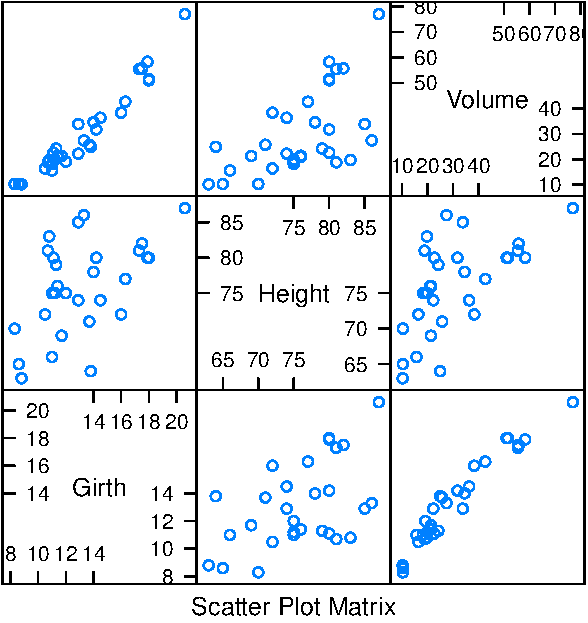
\includegraphics{_main_files/figure-latex/splom-trees-1.pdf}
\caption{\label{fig:splom-trees}\small A scatterplot matrix of the \texttt{trees}
data.}
\end{figure}




The dependent (response) variable \texttt{Volume} is listed in the first
row of the scatterplot matrix. Moving from left to right, we see an
approximately linear relationship between \texttt{Volume} and the
independent (explanatory) variables \texttt{Height} and \texttt{Girth}.
A first guess at a model for these data might be

\begin{equation}
Y=\beta_{0}+\beta_{1}x_{1}+\beta_{2}x_{2}+\epsilon,
\end{equation}

in which case the quantity
\(\mu(x_{1},x_{2})=\beta_{0}+\beta_{1}x_{1}+\beta_{2}x_{2}\) would
represent the mean value of \(Y\) at the point \((x_{1},x_{2})\).

\subsection{What does it mean?}\label{what-does-it-mean}

The interpretation is simple. The intercept \(\beta_{0}\) represents the
mean \texttt{Volume} when all other independent variables are zero. The
parameter \(\beta_{i}\) represents the change in mean \texttt{Volume}
when there is a unit increase in \(x_{i}\), while the other independent
variable is held constant. For the \texttt{trees} data, \(\beta_{1}\)
represents the change in average \texttt{Volume} as \texttt{Girth}
increases by one unit when the \texttt{Height} is held constant, and
\(\beta_{2}\) represents the change in average \texttt{Volume} as
\texttt{Height} increases by one unit when the \texttt{Girth} is held
constant.

In simple linear regression, we had one independent variable and our
linear regression surface was 1D, simply a line. In multiple regression
there are many independent variables and so our linear regression
surface will be many-D\ldots{} in general, a hyperplane. But when there
are only two explanatory variables the hyperplane is just an ordinary
plane and we can look at it with a 3D scatterplot.

One way to do this is with the R Commander in the \texttt{Rcmdr} package
\autocite{Rcmdr}. It has a 3D scatterplot option under the
\texttt{Graphs} menu. It is especially great because the resulting graph
is dynamic; it can be moved around with the mouse, zoomed, \emph{etc}.
But that particular display does not translate well to a printed book.

Another way to do it is with the \texttt{scatterplot3d} function in the
\texttt{scatterplot3d} package \autocite{scatterplot3d}. The code
follows, and the result is shown in Figure
\ref{fig:3D-scatterplot-trees}.

\begin{Shaded}
\begin{Highlighting}[]
\NormalTok{s3d <-}\StringTok{ }\KeywordTok{with}\NormalTok{(trees, }\KeywordTok{scatterplot3d}\NormalTok{(Girth, Height, Volume, }\DataTypeTok{pch =} \DecValTok{16}\NormalTok{, }
                                 \DataTypeTok{highlight.3d =} \OtherTok{TRUE}\NormalTok{, }\DataTypeTok{angle =} \DecValTok{60}\NormalTok{))}
\end{Highlighting}
\end{Shaded}

\begin{figure}[htbp]
\centering
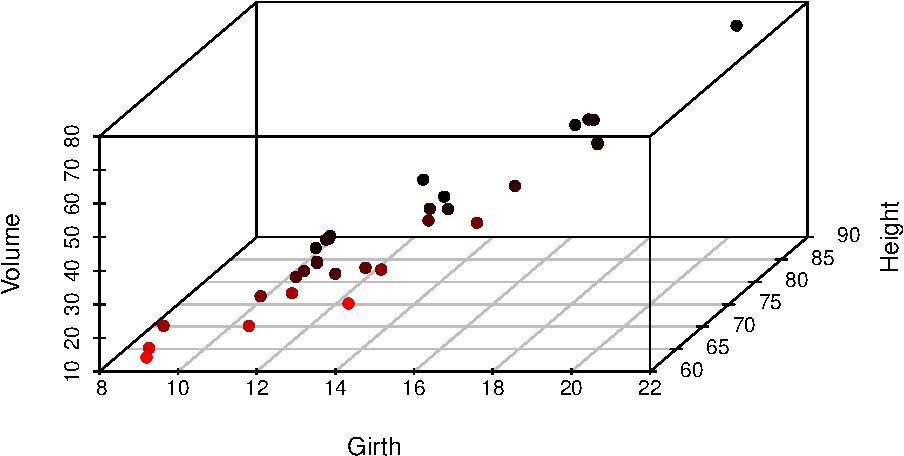
\includegraphics{_main_files/figure-latex/3D-scatterplot-trees-1.pdf}
\caption{\label{fig:3D-scatterplot-trees}(ref:3D-scatterplot-trees)}
\end{figure}




Looking at the graph we see that the data points fall close to a plane
in three dimensional space. (The plot looks remarkably good. In the
author's experience it is rare to see points fit so well to the plane
without some additional work.)

\section{Estimation and
Prediction}\label{sec-estimation-and-prediction-mlr}

\subsection{Parameter estimates}\label{sub-mlr-parameter-estimates}

We will proceed exactly like we did in Section \ref{sec-slr-estimation}.
We know

\begin{equation}
\upepsilon\sim\mathsf{mvnorm}\left(\mathtt{mean}=\mathbf{0}_{\mathrm{n}\times1},\,\mathtt{sigma}=\sigma^{2}\mathbf{I}_{\mathrm{n}\times\mathrm{n}}\right),
\end{equation}

which means that \(\mathbf{Y}=\mathbf{X}\upbeta+\upepsilon\) has an
\(\mathsf{mvnorm}\left(\mathtt{mean}=\mathbf{X}\upbeta,\,\mathtt{sigma}=\sigma^{2}\mathbf{I}_{\mathrm{n}\times\mathrm{n}}\right)\)
distribution. Therefore, the likelihood function
\index{likelihood function} is

\begin{equation}
L(\upbeta,\sigma)=\frac{1}{2\pi^{n/2}\sigma}\exp\left\{ -\frac{1}{2\sigma^{2}}\left(\mathbf{Y}-\mathbf{X}\upbeta\right)^{\mathrm{T}}\left(\mathbf{Y}-\mathbf{X}\upbeta\right)\right\}.
\end{equation}

To \emph{maximize} the likelihood \index{maximum likelihood} in
\(\upbeta\), we need to \emph{minimize} the quantity
\(g(\upbeta)=\left(\mathbf{Y}-\mathbf{X}\upbeta\right)^{\mathrm{T}}\left(\mathbf{Y}-\mathbf{X}\upbeta\right)\).
We do this by differentiating \(g\) with respect to \(\upbeta\). (It may
be a good idea to brush up on the material in Appendices
\ref{sec-linear-algebra} and \ref{sec-multivariable-calculus}.) First we
will rewrite \(g\):

\begin{equation}
g(\upbeta)=\mathbf{Y}^{\mathrm{T}}\mathbf{Y}-\mathbf{Y}^{\mathrm{T}}\mathbf{X}\upbeta-\upbeta^{\mathrm{T}}\mathbf{X}^{\mathrm{T}}\mathbf{Y}+\upbeta^{\mathrm{T}}\mathbf{X}^{\mathrm{T}}\mathbf{X}\upbeta,
\end{equation}

which can be further simplified to
\(g(\upbeta)=\mathbf{Y}^{\mathrm{T}}\mathbf{Y}-2\upbeta^{\mathrm{T}}\mathbf{X}^{\mathrm{T}}\mathbf{Y}+\upbeta^{\mathrm{T}}\mathbf{X}^{\mathrm{T}}\mathbf{X}\upbeta\)
since \(\upbeta^{\mathrm{T}}\mathbf{X}^{\mathrm{T}}\mathbf{Y}\) is
\(1\times1\) and thus equal to its transpose. Now we differentiate to
get

\begin{equation}
\frac{\partial g}{\partial\upbeta}=\mathbf{0}-2\mathbf{X}^{\mathrm{T}}\mathbf{Y}+2\mathbf{X}^{\mathrm{T}}\mathbf{X}\upbeta,
\end{equation}

since \(\mathbf{X}^{\mathrm{T}}\mathbf{X}\) is symmetric. Setting the
derivative equal to the zero vector yields the so called ``normal
equations'' \index{normal equations}

\begin{equation}
\mathbf{X}^{\mathrm{T}}\mathbf{X}\upbeta=\mathbf{X}^{\mathrm{T}}\mathbf{Y}.
\end{equation}

In the case that \(\mathbf{X}^{\mathrm{T}}\mathbf{X}\) is
invertible\footnote{We can find solutions of the normal equations even
  when \(\mathbf{X}^{\mathrm{T}}\mathbf{X}\) is not of full rank, but
  the topic falls outside the scope of this book. The interested reader
  can consult an advanced text such as Rao \autocite{Rao1999}.}, we may
solve the equation for \(\upbeta\) to get the maximum likelihood
estimator of \(\upbeta\) which we denote by \(\mathbf{b}\):

\begin{equation}
\label{eq-b-formula-matrix}
\mathbf{b}=\left(\mathbf{X}^{\mathrm{T}}\mathbf{X}\right)^{-1}\mathbf{X}^{\mathrm{T}}\mathbf{Y}.
\end{equation}

\bigskip

\begin{rem}
The formula in Equation \eqref{eq-b-formula-matrix} is convenient for
mathematical study but is inconvenient for numerical computation.
Researchers have devised much more efficient algorithms for the actual
calculation of the parameter estimates, and we do not explore them here.
\end{rem}

\bigskip

\BeginKnitrBlock{rem}
We have only found a critical value, and have not actually shown that
the critical value is a minimum. We omit the details and refer the
interested reader to \autocite{Rao1999}.
\EndKnitrBlock{rem}

\subsubsection{How to do it with R}\label{how-to-do-it-with-r-34}

We do all of the above just as we would in simple linear regression. The
powerhouse is the \texttt{lm} \index{lm@\texttt{lm}} function.
Everything else is based on it. We separate explanatory variables in the
model formula by a plus sign.

\begin{Shaded}
\begin{Highlighting}[]
\NormalTok{trees.lm <-}\StringTok{ }\KeywordTok{lm}\NormalTok{(Volume ~}\StringTok{ }\NormalTok{Girth +}\StringTok{ }\NormalTok{Height, }\DataTypeTok{data =} \NormalTok{trees)}
\NormalTok{trees.lm}
\end{Highlighting}
\end{Shaded}

\begin{verbatim}

Call:
lm(formula = Volume ~ Girth + Height, data = trees)

Coefficients:
(Intercept)        Girth       Height  
   -57.9877       4.7082       0.3393  
\end{verbatim}

We see from the output that for the \texttt{trees} data our parameter
estimates are \[ \mathbf{b}=\begin{bmatrix}-58.0 & 4.7 &
0.3\end{bmatrix}, \] and consequently our estimate of the mean response
is \(\hat{\mu}\) given by

\begin{alignat}{1} 
\hat{\mu}(x_{1},x_{2}) = & \ b_{0} + b_{1} x_{1} + b_{2}x_{2},\\ \approx & -58.0 + 4.7 x_{1} + 0.3 x_{2}.
\end{alignat}

We could see the entire model matrix \(\mathbf{X}\) with the
\texttt{model.matrix} \index{model.matrix@\texttt{model.matrix}}
function, but in the interest of brevity we only show the first few
rows.

\begin{Shaded}
\begin{Highlighting}[]
\KeywordTok{head}\NormalTok{(}\KeywordTok{model.matrix}\NormalTok{(trees.lm))}
\end{Highlighting}
\end{Shaded}

\begin{verbatim}
  (Intercept) Girth Height
1           1   8.3     70
2           1   8.6     65
3           1   8.8     63
4           1  10.5     72
5           1  10.7     81
6           1  10.8     83
\end{verbatim}

\subsection{Point Estimates of the Regression
Surface}\label{sub-mlr-point-est-regsurface}

The parameter estimates \(\mathbf{b}\) make it easy to find the fitted
values \index{fitted values}, \(\hat{\mathbf{Y}}\). We write them
individually as \(\hat{Y}_{i}\), \(i=1,2,\ldots,n\), and recall that
they are defined by

\begin{eqnarray}
\hat{Y}_{i} & = & \hat{\mu}(x_{1i},x_{2i}),\\
 & = & b_{0}+b_{1}x_{1i}+b_{2}x_{2i},\quad i=1,2,\ldots,n.
\end{eqnarray}

They are expressed more compactly by the matrix equation

\begin{equation}
\hat{\mathbf{Y}}=\mathbf{X}\mathbf{b}.
\end{equation}

From Equation \eqref{eq-b-formula-matrix} we know that
\(\mathbf{b}=\left(\mathbf{X}^{\mathrm{T}}\mathbf{X}\right)^{-1}\mathbf{X}^{\mathrm{T}}\mathbf{Y}\),
so we can rewrite

\begin{eqnarray}
\hat{\mathbf{Y}} & = & \mathbf{X}\left[\left(\mathbf{X}^{\mathrm{T}}\mathbf{X}\right)^{-1}\mathbf{X}^{\mathrm{T}}\mathbf{Y}\right],\\
 & = & \mathbf{H}\mathbf{Y},
\end{eqnarray}

where
\(\mathbf{H}=\mathbf{X}\left(\mathbf{X}^{\mathrm{T}}\mathbf{X}\right)^{-1}\mathbf{X}^{\mathrm{T}}\)
is appropriately named \emph{the hat matrix} \index{hat matrix} because
it ``puts the hat on \(\mathbf{Y}\)''. The hat matrix is very important
in later courses. Some facts about \(\mathbf{H}\) are

\begin{itemize}
\tightlist
\item
  \(\mathbf{H}\) is a symmetric square matrix, of dimension
  \(\mathrm{n}\times\mathrm{n}\).
\item
  The diagonal entries \(h_{ii}\) satisfy \(0\leq h_{ii}\leq1\) (compare
  to Equation \eqref{eq-slr-leverage-between}).
\item
  The trace is \(\mathrm{tr}(\mathbf{H})=p\).
\item
  \(\mathbf{H}\) is \emph{idempotent} (also known as a \emph{projection
  matrix}) which means that \(\mathbf{H}^{2}=\mathbf{H}\). The same is
  true of \(\mathbf{I}-\mathbf{H}\).
\end{itemize}

Now let us write a column vector
\(\mathbf{x}_{0}=(x_{10},x_{20})^{\mathrm{T}}\) to denote given values
of the explanatory variables \texttt{Girth\ ==} \(x_{10}\) and
\texttt{Height\ ==} \(x_{20}\). These values may match those of the
collected data, or they may be completely new values not observed in the
original data set. We may use the parameter estimates to find
\(\hat{Y}(\mathbf{x}_{0})\), which will give us 1. an estimate of
\(\mu(\mathbf{x}_{0})\), the mean value of a future observation at
\(\mathbf{x}_{0}\), and 2. a prediction for \(Y(\mathbf{x}_{0})\), the
actual value of a future observation at \(\mathbf{x}_{0}\).

We can represent \(\hat{Y}(\mathbf{x}_{0})\) by the matrix equation

\begin{equation}
\label{eq-mlr-single-yhat-matrix}
\hat{Y}(\mathbf{x}_{0})=\mathbf{x}_{0}^{\mathrm{T}}\mathbf{b},
\end{equation}

which is just a fancy way to write

\begin{equation}
\hat{Y}(x_{10},x_{20})=b_{0}+b_{1}x_{10}+b_{2}x_{20}.
\end{equation}

\bigskip

\BeginKnitrBlock{example}
\protect\hypertarget{ex:unnamed-chunk-298}{}{\label{ex:unnamed-chunk-298}}If
we wanted to predict the average volume of black cherry trees that have
\texttt{Girth\ =\ 15} in and are \texttt{Height\ =\ 77} ft tall then we
would use the estimate
\EndKnitrBlock{example}

\begin{alignat*}{1}
\hat{\mu}(15,\,77)= & -58+4.7(15)+0.3(77),\\
\approx & 35.6\mbox{\,\ ft}^{3}.
\end{alignat*}

We would use the same estimate \(\hat{Y}=35.6\) to predict the measured
\texttt{Volume} of another black cherry tree -- yet to be observed --
that has \texttt{Girth\ =\ 15} in and is \texttt{Height\ =\ 77} ft tall.

\subsubsection{How to do it with R}\label{how-to-do-it-with-r-35}

The fitted values are stored inside \texttt{trees.lm} and may be
accessed with the \texttt{fitted} function. We only show the first five
fitted values.

\begin{Shaded}
\begin{Highlighting}[]
\KeywordTok{fitted}\NormalTok{(trees.lm)[}\DecValTok{1}\NormalTok{:}\DecValTok{5}\NormalTok{]}
\end{Highlighting}
\end{Shaded}

\begin{verbatim}
        1         2         3         4         5 
 4.837660  4.553852  4.816981 15.874115 19.869008 
\end{verbatim}

The syntax for general prediction does not change much from simple
linear regression. The computations are done with the \texttt{predict}
function as described below.

The only difference from SLR is in the way we tell R the values of the
explanatory variables for which we want predictions. In SLR we had only
one independent variable but in MLR we have many (for the \texttt{trees}
data we have two). We will store values for the independent variables in
the data frame \texttt{new}, which has two columns (one for each
independent variable) and three rows (we shall make predictions at three
different locations).

\begin{Shaded}
\begin{Highlighting}[]
\NormalTok{new <-}\StringTok{ }\KeywordTok{data.frame}\NormalTok{(}\DataTypeTok{Girth =} \KeywordTok{c}\NormalTok{(}\FloatTok{9.1}\NormalTok{, }\FloatTok{11.6}\NormalTok{, }\FloatTok{12.5}\NormalTok{), }\DataTypeTok{Height =} \KeywordTok{c}\NormalTok{(}\DecValTok{69}\NormalTok{, }\DecValTok{74}\NormalTok{, }\DecValTok{87}\NormalTok{))}
\end{Highlighting}
\end{Shaded}

We can view the locations at which we will predict:

\begin{Shaded}
\begin{Highlighting}[]
\NormalTok{new}
\end{Highlighting}
\end{Shaded}

\begin{verbatim}
  Girth Height
1   9.1     69
2  11.6     74
3  12.5     87
\end{verbatim}

We continue just like we would have done in SLR.

\begin{Shaded}
\begin{Highlighting}[]
\KeywordTok{predict}\NormalTok{(trees.lm, }\DataTypeTok{newdata =} \NormalTok{new)}
\end{Highlighting}
\end{Shaded}

\begin{verbatim}
        1         2         3 
 8.264937 21.731594 30.379205 
\end{verbatim}

\textbf{Example.} Using the \texttt{trees} data,

\begin{enumerate}
\def\labelenumi{\arabic{enumi}.}
\tightlist
\item
  Report a point estimate of the mean \texttt{Volume} of a tree of
  \texttt{Girth} 9.1 in and \texttt{Height} 69 ft. The fitted value for
  \(x_{1}=9.1\) and \(x_{2} = 69\) is 8.3, so a point estimate would be
  8.3 cubic feet.
\item
  Report a point prediction for and a 95\% prediction interval for the
  \texttt{Volume} of a hypothetical tree of \texttt{Girth} 12.5 in and
  \texttt{Height} 87 ft. The fitted value for \(x_{1} = 12.5\) and
  \(x_{2} = 87\) is 30.4, so a point prediction for the \texttt{Volume}
  is 30.4 cubic feet.
\end{enumerate}

\subsection{Mean Square Error and Standard Error}\label{sub-mlr-mse-se}

The residuals are given by

\begin{equation}
\mathbf{E}=\mathbf{Y}-\hat{\mathbf{Y}}=\mathbf{Y}-\mathbf{H}\mathbf{Y}=(\mathbf{I}-\mathbf{H})\mathbf{Y}.
\end{equation}

Now we can use Theorem \ref{thm:mvnorm-dist-matrix-prod} to see that the
residuals are distributed

\begin{equation}
\mathbf{E}\sim\mathsf{mvnorm}(\mathtt{mean}=\mathbf{0},\,\mathtt{sigma}=\sigma^{2}(\mathbf{I}-\mathbf{H})),
\end{equation}

since
\((\mathbf{I}-\mathbf{H})\mathbf{X}\upbeta=\mathbf{X}\upbeta-\mathbf{X}\upbeta=\mathbf{0}\)
and
\((\mathbf{I}-\mathbf{H})\,(\sigma^{2}\mathbf{I})\,(\mathbf{I}-\mathbf{H})^{\mathrm{T}}=\sigma^{2}(\mathbf{I}-\mathbf{H})^{2}=\sigma^{2}(\mathbf{I}-\mathbf{H})\).
Thesum of squared errors \(SSE\) is just

\begin{equation}
SSE=\mathbf{E}^{\mathrm{T}}\mathbf{E}=\mathbf{Y}^{\mathrm{T}}(\mathbf{I}-\mathbf{H})(\mathbf{I}-\mathbf{H})\mathbf{Y}=\mathbf{Y}^{\mathrm{T}}(\mathbf{I}-\mathbf{H})\mathbf{Y}.
\end{equation}

Recall that in SLR we had two parameters (\(\beta_{0}\) and
\(\beta_{1}\)) in our regression model and we estimated \(\sigma^{2}\)
with \(s^{2}=SSE/(n-2)\). In MLR, we have \(p+1\) parameters in our
regression model and we might guess that to estimate \(\sigma^{2}\) we
would use the \emph{mean square error} \(S^{2}\) defined by

\begin{equation}
S^{2}=\frac{SSE}{n-(p+1)}.
\end{equation}

That would be a good guess. The \emph{residual standard error} is
\(S=\sqrt{S^{2}}\).

\subsubsection{How to do it with R}\label{how-to-do-it-with-r-36}

The residuals are also stored with \texttt{trees.lm} and may be accessed
with the \texttt{residuals} function. We only show the first five
residuals.

\begin{Shaded}
\begin{Highlighting}[]
\KeywordTok{residuals}\NormalTok{(trees.lm)[}\DecValTok{1}\NormalTok{:}\DecValTok{5}\NormalTok{]}
\end{Highlighting}
\end{Shaded}

\begin{verbatim}
         1          2          3          4          5 
 5.4623403  5.7461484  5.3830187  0.5258848 -1.0690084 
\end{verbatim}

The \texttt{summary} function output (shown later) lists the
\texttt{Residual\ Standard\ Error} which is just \(S=\sqrt{S^{2}}\). It
is stored in the \texttt{sigma} component of the \texttt{summary}
object.

\begin{Shaded}
\begin{Highlighting}[]
\NormalTok{treesumry <-}\StringTok{ }\KeywordTok{summary}\NormalTok{(trees.lm)}
\NormalTok{treesumry$sigma}
\end{Highlighting}
\end{Shaded}

\begin{verbatim}
[1] 3.881832
\end{verbatim}

For the \texttt{trees} data we find \(s \approx\) 3.882.

\subsection{Interval Estimates of the
Parameters}\label{sub-mlr-interval-est-params}

We showed in Section \ref{sub-mlr-parameter-estimates} that
\(\mathbf{b}=\left(\mathbf{X}^{\mathrm{T}}\mathbf{X}\right)^{-1}\mathbf{X}^{\mathrm{T}}\mathbf{Y}\),
which is really just a big matrix -- namely
\(\left(\mathbf{X}^{\mathrm{T}}\mathbf{X}\right)^{-1}\mathbf{X}^{\mathrm{T}}\)
-- multiplied by \(\mathbf{Y}\). It stands to reason that the sampling
distribution of \(\mathbf{b}\) would be intimately related to the
distribution of \(\mathbf{Y}\), which we assumed to be

\begin{equation}
\mathbf{Y}\sim\mathsf{mvnorm}\left(\mathtt{mean}=\mathbf{X}\upbeta,\,\mathtt{sigma}=\sigma^{2}\mathbf{I}\right).
\end{equation}

Now recall Theorem \ref{thm:mvnorm-dist-matrix-prod} that we said we
were going to need eventually (the time is now). That proposition
guarantees that

\begin{equation}
\label{eq-distn-b-mlr}
\mathbf{b}\sim\mathsf{mvnorm}\left(\mathtt{mean}=\upbeta,\,\mathtt{sigma}=\sigma^{2}\left(\mathbf{X}^{\mathrm{T}}\mathbf{X}\right)^{-1}\right),
\end{equation}

since

\begin{equation}
\mathbb{E}\mathbf{b}=\left(\mathbf{X}^{\mathrm{T}}\mathbf{X}\right)^{-1}\mathbf{X}^{\mathrm{T}}(\mathbf{X}\upbeta)=\upbeta,
\end{equation}

and

\begin{equation}
\mbox{Var}(\mathbf{b})=\left(\mathbf{X}^{\mathrm{T}}\mathbf{X}\right)^{-1}\mathbf{X}^{\mathrm{T}}(\sigma^{2}\mathbf{I})\mathbf{X}\left(\mathbf{X}^{\mathrm{T}}\mathbf{X}\right)^{-1}=\sigma^{2}\left(\mathbf{X}^{\mathrm{T}}\mathbf{X}\right)^{-1},
\end{equation}

the first equality following because the matrix
\(\left(\mathbf{X}^{\mathrm{T}}\mathbf{X}\right)^{-1}\) is symmetric.

There is a lot that we can glean from Equation \eqref{eq-distn-b-mlr}.
First, it follows that the estimator \(\mathbf{b}\) is unbiased (see
Section \ref{sec-point-estimation-1}). Second, the variances of
\(b_{0}\), \(b_{1}\), \ldots{}, \(b_{n}\) are exactly the diagonal
elements of
\(\sigma^{2}\left(\mathbf{X}^{\mathrm{T}}\mathbf{X}\right)^{-1}\), which
is completely known except for that pesky parameter \(\sigma^{2}\).
Third, we can estimate the standard error of \(b_{i}\) (denoted
\(S_{b_{i}}\)) with the mean square error \(S\) (defined in the previous
section) multiplied by the corresponding diagonal element of
\(\left(\mathbf{X}^{\mathrm{T}}\mathbf{X}\right)^{-1}\). Finally, given
estimates of the standard errors we may construct confidence intervals
for \(\beta_{i}\) with an interval that looks like

\begin{equation}
b_{i}\pm\mathsf{t}_{\alpha/2}(\mathtt{df}=n-p-1)S_{b_{i}}.
\end{equation}

The degrees of freedom for the Student's \(t\) distribution\footnote{We
  are taking great leaps over the mathematical details. In particular,
  we have yet to show that \(s^{2}\) has a chi-square distribution and
  we have not even come close to showing that \(b_{i}\) and
  \(s_{b_{i}}\) are independent. But these are entirely outside the
  scope of the present book and the reader may rest assured that the
  proofs await in later classes. See C.R. Rao for more.} are the same as
the denominator of \(S^{2}\).

\subsubsection{How to do it with R}\label{how-to-do-it-with-r-37}

To get confidence intervals for the parameters we need only use
\texttt{confint} \index{confint@\texttt{confint}}:

\begin{Shaded}
\begin{Highlighting}[]
\KeywordTok{confint}\NormalTok{(trees.lm)}
\end{Highlighting}
\end{Shaded}

\begin{verbatim}
                   2.5 %      97.5 %
(Intercept) -75.68226247 -40.2930554
Girth         4.16683899   5.2494820
Height        0.07264863   0.6058538
\end{verbatim}

For example, using the calculations above we say that for the regression
model \texttt{Volume\ \textasciitilde{}\ Girth\ +\ Height} we are 95\%
confident that the parameter \(\beta_{1}\) lies somewhere in the
interval 4.2 to 5.2.

\subsection{Confidence and Prediction
Intervals}\label{confidence-and-prediction-intervals}

We saw in Section \ref{sub-mlr-point-est-regsurface} how to make point
estimates of the mean value of additional observations and predict
values of future observations, but how good are our estimates? We need
confidence and prediction intervals to gauge their accuracy, and lucky
for us the formulas look similar to the ones we saw in SLR.

In Equation \eqref{eq-mlr-single-yhat-matrix} we wrote
\(\hat{Y}(\mathbf{x}_0)=\mathbf{x}_0^{\mathrm{T}}\mathbf{b}\), and in
Equation \eqref{eq-distn-b-mlr} we saw that

\begin{equation}
\mathbf{b}\sim\mathsf{mvnorm}\left(\mathtt{mean} = \upbeta,\,\mathtt{sigma}=\sigma^{2}\left(\mathbf{X}^{\mathrm{T}}\mathbf{X}\right)^{-1}\right).
\end{equation}

The following is therefore immediate from Theorem
\ref{thm:mvnorm-dist-matrix-prod}:

\begin{equation}
\hat{Y}(\mathbf{x}_{0})\sim\mathsf{mvnorm}\left(\mathtt{mean}=\mathbf{x}_{0}^{\mathrm{T}}\upbeta,\,\mathtt{sigma}=\sigma^{2}\mathbf{x}_{0}^{\mathrm{T}}\left(\mathbf{X}^{\mathrm{T}}\mathbf{X}\right)^{-1}\mathbf{x}_{0}\right).
\end{equation}

It should be no surprise that confidence intervals for the mean value of
a future observation at the location
\(\mathbf{x}_{0}=\begin{bmatrix}x_{10} & x_{20} & \ldots & x_{p0}\end{bmatrix}^{\mathrm{T}}\)
are given by

\begin{equation}
\hat{Y}(\mathbf{x}_{0})\pm\mathsf{t}_{\alpha/2}(\mathtt{df}=n-p-1)\, S\sqrt{\mathbf{x}_{0}^{\mathrm{T}}\left(\mathbf{X}^{\mathrm{T}}\mathbf{X}\right)^{-1}\mathbf{x}_{0}}.
\end{equation}

Intuitively,
\(\mathbf{x}_{0}^{\mathrm{T}}\left(\mathbf{X}^{\mathrm{T}}\mathbf{X}\right)^{-1}\mathbf{x}_{0}\)
measures the distance of \(\mathbf{x}_{0}\) from the center of the data.
The degrees of freedom in the Student's \(t\) critical value are
\(n-(p+1)\) because we need to estimate \(p+1\) parameters.

Prediction intervals for a new observation at \(\mathbf{x}_{0}\) are
given by

\begin{equation}
\hat{Y}(\mathbf{x}_{0})\pm\mathsf{t}_{\alpha/2}(\mathtt{df}=n-p-1)\, S\sqrt{1+\mathbf{x}_{0}^{\mathrm{T}}\left(\mathbf{X}^{\mathrm{T}}\mathbf{X}\right)^{-1}\mathbf{x}_{0}}.
\end{equation}

The prediction intervals are wider than the confidence intervals, just
as in Section \ref{sub-slr-interval-est-regline}.

\subsubsection{How to do it with R}\label{how-to-do-it-with-r-38}

The syntax is identical to that used in SLR, with the proviso that we
need to specify values of the independent variables in the data frame
\texttt{new} as we did in Section \ref{sub-slr-interval-est-regline}
(which we repeat here for illustration).

\begin{Shaded}
\begin{Highlighting}[]
\NormalTok{new <-}\StringTok{ }\KeywordTok{data.frame}\NormalTok{(}\DataTypeTok{Girth =} \KeywordTok{c}\NormalTok{(}\FloatTok{9.1}\NormalTok{, }\FloatTok{11.6}\NormalTok{, }\FloatTok{12.5}\NormalTok{), }\DataTypeTok{Height =} \KeywordTok{c}\NormalTok{(}\DecValTok{69}\NormalTok{, }\DecValTok{74}\NormalTok{, }\DecValTok{87}\NormalTok{))}
\end{Highlighting}
\end{Shaded}

Confidence intervals are given by

\begin{Shaded}
\begin{Highlighting}[]
\KeywordTok{predict}\NormalTok{(trees.lm, }\DataTypeTok{newdata =} \NormalTok{new, }\DataTypeTok{interval =} \StringTok{"confidence"}\NormalTok{)}
\end{Highlighting}
\end{Shaded}

\begin{verbatim}
        fit      lwr      upr
1  8.264937  5.77240 10.75747
2 21.731594 20.11110 23.35208
3 30.379205 26.90964 33.84877
\end{verbatim}

Prediction intervals are given by

\begin{Shaded}
\begin{Highlighting}[]
\KeywordTok{predict}\NormalTok{(trees.lm, }\DataTypeTok{newdata =} \NormalTok{new, }\DataTypeTok{interval =} \StringTok{"prediction"}\NormalTok{)}
\end{Highlighting}
\end{Shaded}

\begin{verbatim}
        fit         lwr      upr
1  8.264937 -0.06814444 16.59802
2 21.731594 13.61657775 29.84661
3 30.379205 21.70364103 39.05477
\end{verbatim}

As before, the interval type is decided by the \texttt{interval}
argument and the default confidence level is 95\% (which can be changed
with the \texttt{level} argument).

\textbf{Example.} Using the \texttt{trees} data,

\begin{enumerate}
\def\labelenumi{\arabic{enumi}.}
\tightlist
\item
  Report a 95\% confidence interval for the mean \texttt{Volume} of a
  tree of \texttt{Girth} 9.1 in and \texttt{Height} 69 ft. The 95\% CI
  is given by 5.8 to 10.8, so with 95\% confidence the mean
  \texttt{Volume} lies somewhere between 5.8 cubic feet and 10.8 cubic
  feet.
\item
  Report a 95\% prediction interval for the \texttt{Volume} of a
  hypothetical tree of \texttt{Girth} 12.5 in and \texttt{Height} 87 ft.
  The 95\% prediction interval is given by 26.9 to 33.8, so with 95\%
  confidence we may assert that the hypothetical \texttt{Volume} of a
  tree of \texttt{Girth} 12.5 in and \texttt{Height} 87 ft would lie
  somewhere between 26.9 cubic feet and 33.8 feet.
\end{enumerate}

\section{Model Utility and Inference}\label{sec-model-utility-and-mlr}

\subsection{Multiple Coefficient of
Determination}\label{multiple-coefficient-of-determination}

We saw in Section \ref{sub-mlr-mse-se} that the error sum of squares
\(SSE\) can be conveniently written in MLR as

\begin{equation}
\label{eq-mlr-sse-matrix}
SSE=\mathbf{Y}^{\mathrm{T}}(\mathbf{I}-\mathbf{H})\mathbf{Y}.
\end{equation}

It turns out that there are equally convenient formulas for the total
sum of squares \(SSTO\) and the regression sum of squares \(SSR\). They
are:

\begin{alignat}{1}
\label{eq-mlr-ssto-matrix}
SSTO= & \mathbf{Y}^{\mathrm{T}}\left(\mathbf{I}-\frac{1}{n}\mathbf{J}\right)\mathbf{Y}
\end{alignat}

and

\begin{alignat}{1}
\label{eq-mlr-ssr-matrix}
SSR= & \mathbf{Y}^{\mathrm{T}}\left(\mathbf{H}-\frac{1}{n}\mathbf{J}\right)\mathbf{Y}.
\end{alignat}

(The matrix \(\mathbf{J}\) is defined in Appendix
\ref{sec-linear-algebra}.) Immediately from Equations
\eqref{eq-mlr-sse-matrix}, \eqref{eq-mlr-ssto-matrix}, and
\eqref{eq-mlr-ssr-matrix} we get the \emph{Anova Equality}

\begin{equation} 
SSTO=SSE+SSR.
\end{equation}

(See Exercise \ref{xca-anova-equality}.) We define the \emph{multiple
coefficient of determination} by the formula

\begin{equation} 
R^{2}=1-\frac{SSE}{SSTO}.
\end{equation}

We interpret \(R^{2}\) as the proportion of total variation that is
explained by the multiple regression model. In MLR we must be careful,
however, because the value of \(R^{2}\) can be artificially inflated by
the addition of explanatory variables to the model, regardless of
whether or not the added variables are useful with respect to prediction
of the response variable. In fact, it can be proved that the addition of
a single explanatory variable to a regression model will increase the
value of \(R^{2}\), \emph{no matter how worthless} the explanatory
variable is. We could model the height of the ocean tides, then add a
variable for the length of cheetah tongues on the Serengeti plain, and
our \(R^{2}\) would inevitably increase.

This is a problem, because as the philosopher, Occam, once said:
``causes should not be multiplied beyond necessity''. We address the
problem by penalizing \(R^{2}\) when parameters are added to the model.
The result is an \emph{adjusted} \(R^{2}\) which we denote by
\(\overline{R}^{2}\).

\begin{equation}
\overline{R}^{2}=\left(R^{2}-\frac{p}{n-1}\right)\left(\frac{n-1}{n-p-1}\right).
\end{equation}

It is good practice for the statistician to weigh both \(R^{2}\) and
\(\overline{R}^{2}\) during assessment of model utility. In many cases
their values will be very close to each other. If their values differ
substantially, or if one changes dramatically when an explanatory
variable is added, then (s)he should take a closer look at the
explanatory variables in the model.

\subsubsection{How to do it with R}\label{how-to-do-it-with-r-39}

For the \texttt{trees} data, we can get \(R^{2}\) and
\(\overline{R}^{2}\) from the \texttt{summary} output or access the
values directly by name as shown (recall that we stored the
\texttt{summary} object in \texttt{treesumry}).

\begin{Shaded}
\begin{Highlighting}[]
\NormalTok{treesumry$r.squared}
\end{Highlighting}
\end{Shaded}

\begin{verbatim}
[1] 0.94795
\end{verbatim}

\begin{Shaded}
\begin{Highlighting}[]
\NormalTok{treesumry$adj.r.squared}
\end{Highlighting}
\end{Shaded}

\begin{verbatim}
[1] 0.9442322
\end{verbatim}

High values of \(R^{2}\) and \(\overline{R}^2\) such as these indicate
that the model fits very well, which agrees with what we saw in Figure
\ref{fig:3D-scatterplot-trees}.

\subsection{Overall F-Test}\label{sub-mlr-overall-f-test}

Another way to assess the model's utility is to to test the hypothesis
\[ H_{0}:\beta_{1}=\beta_{2}=\cdots=\beta_{p}=0\mbox{ versus
}H_{1}:\mbox{ at least one $\beta_{i}\neq0$}.  \] The idea is that if
all \(\beta_{i}\)'s were zero, then the explanatory variables
\(X_{1},\ldots,X_{p}\) would be worthless predictors for the response
variable \(Y\). We can test the above hypothesis with the overall \(F\)
statistic, which in MLR is defined by

\begin{equation}
F=\frac{SSR/p}{SSE/(n-p-1)}.
\end{equation}

When the regression assumptions hold and under \(H_{0}\), it can be
shown that \(F\sim\mathsf{f}(\mathtt{df1}=p,\,\mathtt{df2}=n-p-1)\). We
reject \(H_{0}\) when \(F\) is large, that is, when the explained
variation is large relative to the unexplained variation.

\subsubsection{How to do it with R}\label{how-to-do-it-with-r-40}

The overall \(F\) statistic and its associated \emph{p}-value is listed
at the bottom of the \texttt{summary} output, or we can access it
directly by name; it is stored in the \texttt{fstatistic} component of
the \texttt{summary} object.

\begin{Shaded}
\begin{Highlighting}[]
\NormalTok{treesumry$fstatistic}
\end{Highlighting}
\end{Shaded}

\begin{verbatim}
   value    numdf    dendf 
254.9723   2.0000  28.0000 
\end{verbatim}

For the \texttt{trees} data, we see that ( F = ) 254.9723374 with a
\emph{p}-value =\textless{} \texttt{2.2e-16}. Consequently we reject
\(H_{0}\), that is, the data provide strong evidence that not all
\(\beta_{i}\)'s are zero.

\subsection{Student's t Tests}\label{sub-mlr-students-t-tests}

We know that

\begin{equation}
\mathbf{b}\sim\mathsf{mvnorm}\left(\mathtt{mean}=\upbeta,\,\mathtt{sigma}=\sigma^{2}\left(\mathbf{X}^{\mathrm{T}}\mathbf{X}\right)^{-1}\right)
\end{equation}

and we have seen how to test the hypothesis
\(H_{0}:\beta_{1}=\beta_{2}=\cdots=\beta_{p}=0\), but let us now
consider the test

\begin{equation}
H_{0}:\beta_{i}=0\mbox{ versus }H_{1}:\beta_{i}\neq0,
\end{equation}

where \(\beta_{i}\) is the coefficient for the \(i^{\textrm{th}}\)
independent variable. We test the hypothesis by calculating a statistic,
examining it's null distribution, and rejecting \(H_{0}\) if the
\emph{p}-value is small. If \(H_{0}\) is rejected, then we conclude that
there is a significant relationship between \(Y\) and \(x_{i}\) \emph{in
the regression model} \(Y\sim(x_{1},\ldots,x_{p})\). This last part of
the sentence is very important because the significance of the variable
\(x_{i}\) sometimes depends on the presence of other independent
variables in the model\footnote{In other words, a variable might be
  highly significant one moment but then fail to be significant when
  another variable is added to the model. When this happens it often
  indicates a problem with the explanatory variables, such as
  \emph{multicollinearity}. See Section \ref{sub-Multicollinearity}.}.

To test the hypothesis we go to find the sampling distribution of (
b\_\{i\} ), the estimator of the corresponding parameter \(\beta_{i}\),
when the null hypothesis is true. We saw in Section
\ref{sub-mlr-interval-est-params} that

\begin{equation}
T_{i}=\frac{b_{i}-\beta_{i}}{S_{b_{i}}}
\end{equation}

has a Student's \(t\) distribution with \(n-(p+1)\) degrees of freedom.
(Remember, we are estimating \(p+1\) parameters.) Consequently, under
the null hypothesis \(H_{0}:\beta_{i}=0\) the statistic
\(t_{i}=b_{i}/S_{b_{i}}\) has a \(\mathsf{t}(\mathtt{df}=n-p-1)\)
distribution.

\subsubsection{How to do it with R}\label{how-to-do-it-with-r-41}

The Student's \(t\) tests for significance of the individual explanatory
variables are shown in the \texttt{summary} output.

\begin{Shaded}
\begin{Highlighting}[]
\NormalTok{treesumry}
\end{Highlighting}
\end{Shaded}

\begin{verbatim}

Call:
lm(formula = Volume ~ Girth + Height, data = trees)

Residuals:
    Min      1Q  Median      3Q     Max 
-6.4065 -2.6493 -0.2876  2.2003  8.4847 

Coefficients:
            Estimate Std. Error t value Pr(>|t|)    
(Intercept) -57.9877     8.6382  -6.713 2.75e-07 ***
Girth         4.7082     0.2643  17.816  < 2e-16 ***
Height        0.3393     0.1302   2.607   0.0145 *  
---
Signif. codes:  
0 '***' 0.001 '**' 0.01 '*' 0.05 '.' 0.1 ' ' 1

Residual standard error: 3.882 on 28 degrees of freedom
Multiple R-squared:  0.948, Adjusted R-squared:  0.9442 
F-statistic:   255 on 2 and 28 DF,  p-value: < 2.2e-16
\end{verbatim}

We see from the \emph{p-values} that there is a significant linear
relationship between \texttt{Volume} and \texttt{Girth} and between
\texttt{Volume} and \texttt{Height} in the regression model
\texttt{Volume\ \textasciitilde{}\ Girth\ +\ Height}. Further, it
appears that the \texttt{Intercept} is significant in the aforementioned
model.

\section{Polynomial Regression}\label{sec-polynomial-regression}

\subsection{Quadratic Regression
Model}\label{quadratic-regression-model}

In each of the previous sections we assumed that \(\mu\) was a linear
function of the explanatory variables. For example, in SLR we assumed
that \(\mu(x)=\beta_{0}+\beta_{1}x\), and in our previous MLR examples
we assumed
\(\mu(x_{1},x_{2}) = \beta_{0}+\beta_{1}x_{1} + \beta_{2}x_{2}\). In
every case the scatterplots indicated that our assumption was
reasonable. Sometimes, however, plots of the data suggest that the
linear model is incomplete and should be modified.

\begin{Shaded}
\begin{Highlighting}[]
\KeywordTok{plot}\NormalTok{(Volume ~}\StringTok{ }\NormalTok{Girth, }\DataTypeTok{data =} \NormalTok{trees)}
\end{Highlighting}
\end{Shaded}

\begin{figure}[htbp]
\centering
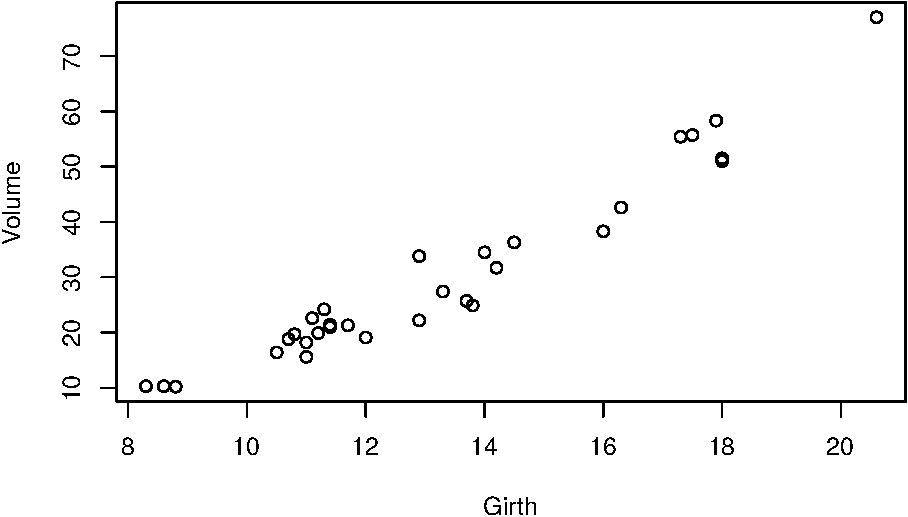
\includegraphics{_main_files/figure-latex/scatterplot-volume-girth-trees-1.pdf}
\caption{\label{fig:scatterplot-volume-girth-trees}\small Scatterplot of
\texttt{Volume} versus \texttt{Girth} for the \texttt{trees} data.}
\end{figure}




For example, let us examine a scatterplot of \texttt{Volume} versus
\texttt{Girth} a little more closely. See Figure
\ref{fig:scatterplot-volume-girth-trees}. There might be a slight
curvature to the data; the volume curves ever so slightly upward as the
girth increases. After looking at the plot we might try to capture the
curvature with a mean response such as

\begin{equation}
\mu(x_{1})=\beta_{0}+\beta_{1}x_{1}+\beta_{2}x_{1}^{2}.
\end{equation}

The model associated with this choice of \(\mu\) is

\begin{equation}
Y=\beta_{0}+\beta_{1}x_{1}+\beta_{2}x_{1}^{2}+\epsilon.
\end{equation}

The regression assumptions are the same. Almost everything indeed is the
same. In fact, it is still called a ``linear regression model'', since
the mean response \(\mu\) is linear \emph{in the parameters}
\(\beta_{0}\), \(\beta_{1}\), and \(\beta_{2}\).

\emph{However, there is one important difference.} When we introduce the
squared variable in the model we inadvertently also introduce strong
dependence between the terms which can cause significant numerical
problems when it comes time to calculate the parameter estimates.
Therefore, we should usually rescale the independent variable to have
mean zero (and even variance one if we wish) \emph{before} fitting the
model. That is, we replace the \(x_{i}\)'s with \(x_{i}-\overline{x}\)
(or \((x_{i}-\overline{x})/s\)) before fitting the model\footnote{Rescaling
  the data gets the job done but a better way to avoid the
  multicollinearity introduced by the higher order terms is with
  \emph{orthogonal polynomials}, whose coefficients are chosen just
  right so that the polynomials are not correlated with each other. This
  is beginning to linger outside the scope of this book, however, so we
  will content ourselves with a brief mention and then stick with the
  rescaling approach in the discussion that follows. A nice example of
  orthogonal polynomials in action can be run with
  \texttt{example(cars)}.}.

\subsubsection{How to do it with R}\label{how-to-do-it-with-r-42}

There are multiple ways to fit a quadratic model to the variables
\texttt{Volume} and \texttt{Girth} using R. 1. One way would be to
square the values for \texttt{Girth} and save them in a vector
\texttt{Girthsq}. Next, fit the linear model
\texttt{Volume\ \textasciitilde{}\ Girth\ +\ \ \ \ Girthsq}. 2. A second
way would be to use the \emph{insulate} function in R, denoted by
\texttt{I}: : Volume \textasciitilde{} Girth + I(Girth\^{}2) The second
method is shorter than the first but the end result is the same. And
once we calculate and store the fitted model (in, say,
\texttt{treesquad.lm}) all of the previous comments regarding R apply.
3. A third and ``right'' way to do it is with orthogonal polynomials: :
Volume \textasciitilde{} poly(Girth, degree = 2) See \texttt{?poly} and
\texttt{?cars} for more information. Note that we can recover the
approach in 2 with
\texttt{poly(Girth,\ degree\ =\ 2,\ raw\ =\ \ \ \ TRUE)}.

\bigskip

\BeginKnitrBlock{example}
\protect\hypertarget{ex:unnamed-chunk-317}{}{\label{ex:unnamed-chunk-317}}We
will fit the quadratic model to the \texttt{trees} data and display the
results with \texttt{summary}, being careful to rescale the data before
fitting the model. We may rescale the \texttt{Girth} variable to have
zero mean and unit variance on-the-fly with the \texttt{scale} function.
\EndKnitrBlock{example}

\begin{Shaded}
\begin{Highlighting}[]
\NormalTok{treesquad.lm <-}\StringTok{ }\KeywordTok{lm}\NormalTok{(Volume ~}\StringTok{ }\KeywordTok{scale}\NormalTok{(Girth) +}\StringTok{ }\KeywordTok{I}\NormalTok{(}\KeywordTok{scale}\NormalTok{(Girth)^}\DecValTok{2}\NormalTok{), }\DataTypeTok{data =} \NormalTok{trees)}
\KeywordTok{summary}\NormalTok{(treesquad.lm)}
\end{Highlighting}
\end{Shaded}

\begin{verbatim}

Call:
lm(formula = Volume ~ scale(Girth) + I(scale(Girth)^2), data = trees)

Residuals:
    Min      1Q  Median      3Q     Max 
-5.4889 -2.4293 -0.3718  2.0764  7.6447 

Coefficients:
                  Estimate Std. Error t value Pr(>|t|)    
(Intercept)        27.7452     0.8161  33.996  < 2e-16 ***
scale(Girth)       14.5995     0.6773  21.557  < 2e-16 ***
I(scale(Girth)^2)   2.5067     0.5729   4.376 0.000152 ***
---
Signif. codes:  
0 '***' 0.001 '**' 0.01 '*' 0.05 '.' 0.1 ' ' 1

Residual standard error: 3.335 on 28 degrees of freedom
Multiple R-squared:  0.9616,    Adjusted R-squared:  0.9588 
F-statistic: 350.5 on 2 and 28 DF,  p-value: < 2.2e-16
\end{verbatim}

We see that the \(F\) statistic indicates the overall model including
\texttt{Girth} and \texttt{Girth\^{}2} is significant. Further, there is
strong evidence that both \texttt{Girth} and \texttt{Girth\^{}2} are
significantly related to \texttt{Volume}. We may examine a scatterplot
together with the fitted quadratic function using the \texttt{lines}
function, which adds a line to the plot tracing the estimated mean
response.

\begin{Shaded}
\begin{Highlighting}[]
\KeywordTok{plot}\NormalTok{(Volume ~}\StringTok{ }\KeywordTok{scale}\NormalTok{(Girth), }\DataTypeTok{data =} \NormalTok{trees)}
\KeywordTok{lines}\NormalTok{(}\KeywordTok{fitted}\NormalTok{(treesquad.lm) ~}\StringTok{ }\KeywordTok{scale}\NormalTok{(Girth), }\DataTypeTok{data =} \NormalTok{trees)}
\end{Highlighting}
\end{Shaded}

\begin{figure}[htbp]
\centering
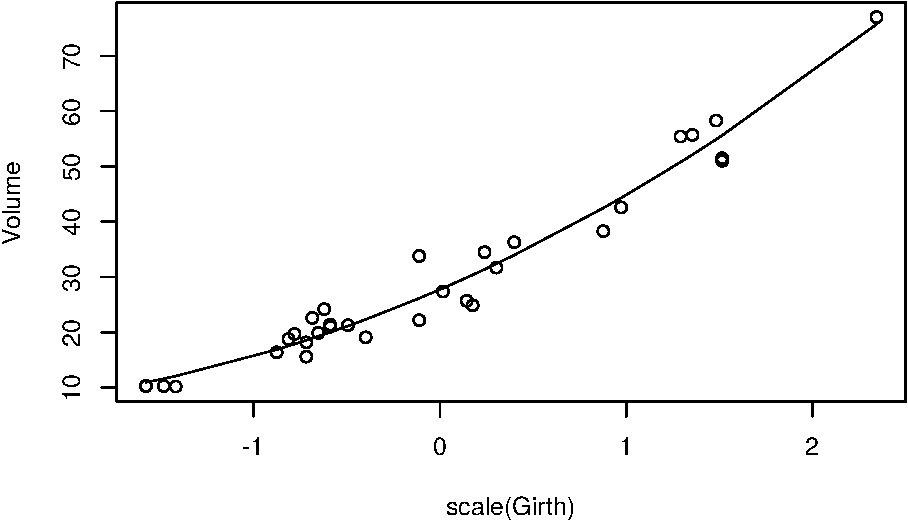
\includegraphics{_main_files/figure-latex/fitting-the-quadratic-1.pdf}
\caption{\label{fig:fitting-the-quadratic}\small A quadratic model for the
\texttt{trees} data.}
\end{figure}




The plot is shown in Figure \ref{fig:fitting-the-quadratic}. Pay
attention to the scale on the \(x\)-axis: it is on the scale of the
transformed \texttt{Girth} data and not on the original scale.

\bigskip

\begin{rem}
When a model includes a quadratic term for an independent variable, it
is customary to also include the linear term in the model. The principle
is called \emph{parsimony}. More generally, if the researcher decides to
include \(x^{m}\) as a term in the model, then (s)he should also include
all lower order terms \(x\), \(x^{2}\), \ldots{},\(x^{m-1}\) in the
model.
\end{rem}

We do estimation/prediction the same way that we did in Section
\ref{sub-mlr-point-est-regsurface}, except we do not need a
\texttt{Height} column in the dataframe =new= since the variable is not
included in the quadratic model.

\begin{Shaded}
\begin{Highlighting}[]
\NormalTok{new <-}\StringTok{ }\KeywordTok{data.frame}\NormalTok{(}\DataTypeTok{Girth =} \KeywordTok{c}\NormalTok{(}\FloatTok{9.1}\NormalTok{, }\FloatTok{11.6}\NormalTok{, }\FloatTok{12.5}\NormalTok{))}
\KeywordTok{predict}\NormalTok{(treesquad.lm, }\DataTypeTok{newdata =} \NormalTok{new, }\DataTypeTok{interval =} \StringTok{"prediction"}\NormalTok{)}
\end{Highlighting}
\end{Shaded}

\begin{verbatim}
       fit       lwr      upr
1 11.56982  4.347426 18.79221
2 20.30615 13.299050 27.31325
3 25.92290 18.972934 32.87286
\end{verbatim}

The predictions and intervals are slightly different from what they were
previously. Notice that it was not necessary to rescale the
\texttt{Girth} prediction data before input to the \texttt{predict}
function; the model did the rescaling for us automatically.

\bigskip

\begin{rem}
We have mentioned on several occasions that it is important to rescale
the explanatory variables for polynomial regression. Watch what happens
if we ignore this advice:
\end{rem}

\begin{Shaded}
\begin{Highlighting}[]
\KeywordTok{summary}\NormalTok{(}\KeywordTok{lm}\NormalTok{(Volume ~}\StringTok{ }\NormalTok{Girth +}\StringTok{ }\KeywordTok{I}\NormalTok{(Girth^}\DecValTok{2}\NormalTok{), }\DataTypeTok{data =} \NormalTok{trees))}
\end{Highlighting}
\end{Shaded}

\begin{verbatim}

Call:
lm(formula = Volume ~ Girth + I(Girth^2), data = trees)

Residuals:
    Min      1Q  Median      3Q     Max 
-5.4889 -2.4293 -0.3718  2.0764  7.6447 

Coefficients:
            Estimate Std. Error t value Pr(>|t|)    
(Intercept) 10.78627   11.22282   0.961 0.344728    
Girth       -2.09214    1.64734  -1.270 0.214534    
I(Girth^2)   0.25454    0.05817   4.376 0.000152 ***
---
Signif. codes:  
0 '***' 0.001 '**' 0.01 '*' 0.05 '.' 0.1 ' ' 1

Residual standard error: 3.335 on 28 degrees of freedom
Multiple R-squared:  0.9616,    Adjusted R-squared:  0.9588 
F-statistic: 350.5 on 2 and 28 DF,  p-value: < 2.2e-16
\end{verbatim}

Now nothing is significant in the model except \texttt{Girth\^{}2}. We
could delete the \texttt{Intercept} and \texttt{Girth} from the model,
but the model would no longer be \emph{parsimonious}. A novice may see
the output and be confused about how to proceed, while the seasoned
statistician recognizes immediately that \texttt{Girth} and
\texttt{Girth\^{}2} are highly correlated (see Section
\ref{sub-multicollinearity}). The only remedy to this ailment is to
rescale \texttt{Girth}, which we should have done in the first place.

In Example \ref{ex:mlr-trees-poly-no-rescale} of Section
\ref{sec-partial-f-statistic}.

\textbf{Note:} The \texttt{trees} data do not have any qualitative
explanatory variables, so we will construct one for illustrative
purposes\footnote{This procedure of replacing a continuous variable by a
  discrete/qualitative one is called \emph{binning}, and is almost
  \emph{never} the right thing to do. We are in a bind at this point,
  however, because we have invested this chapter in the \texttt{trees}
  data and I do not want to switch mid-discussion. I am currently
  searching for a data set with pre-existing qualitative variables that
  also conveys the same points present in the trees data, and when I
  find it I will update this chapter accordingly.}. We will leave the
\texttt{Girth} variable alone, but we will replace the variable
\texttt{Height} by a new variable \texttt{Tall} which indicates whether
or not the cherry tree is taller than a certain threshold (which for the
sake of argument will be the sample median height of 76 ft). That is,
\texttt{Tall} will be defined by

\begin{equation} \mathtt{Tall} = \begin{cases} \mathtt{yes}, & \mbox{if }\mathtt{Height} > 76,\\ \mathtt{no}, & \mbox{if }\mathtt{Height}\leq 76. \end{cases} \end{equation}

We can construct \texttt{Tall} very quickly in R with the \texttt{cut}
function:

\begin{Shaded}
\begin{Highlighting}[]
\NormalTok{trees$Tall <-}\StringTok{ }\KeywordTok{cut}\NormalTok{(trees$Height, }\DataTypeTok{breaks =} \KeywordTok{c}\NormalTok{(-}\OtherTok{Inf}\NormalTok{, }\DecValTok{76}\NormalTok{, }\OtherTok{Inf}\NormalTok{), }
                  \DataTypeTok{labels =} \KeywordTok{c}\NormalTok{(}\StringTok{"no"}\NormalTok{,}\StringTok{"yes"}\NormalTok{))}
\NormalTok{trees$Tall[}\DecValTok{1}\NormalTok{:}\DecValTok{5}\NormalTok{]}
\end{Highlighting}
\end{Shaded}

\begin{verbatim}
[1] no  no  no  no  yes
Levels: no yes
\end{verbatim}

Note that \texttt{Tall} is automatically generated to be a factor with
the labels in the correct order. See \texttt{?cut} for more.

Once we have \texttt{Tall}, we include it in the regression model just
like we would any other variable. It is handled internally in a special
way. Define a ``dummy variable'' \texttt{Tallyes} that takes values

\begin{equation} \mathtt{Tallyes} = \begin{cases} 1, & \mbox{if }\mathtt{Tall}=\mathtt{yes},\\ 0, & \mbox{otherwise.} \end{cases} \end{equation}

That is, \texttt{Tallyes} is an \emph{indicator variable} which
indicates when a respective tree is tall. The model may now be written
as

\begin{equation}
\mathtt{Volume}=\beta_{0}+\beta_{1}\mathtt{Girth}+\beta_{2}\mathtt{Tallyes}+\epsilon.
\end{equation}

Let us take a look at what this definition does to the mean response.
Trees with \texttt{Tall\ =\ yes} will have the mean response

\begin{equation}
\mu(\mathtt{Girth})=(\beta_{0}+\beta_{2})+\beta_{1}\mathtt{Girth},
\end{equation}

while trees with \texttt{Tall\ =\ no} will have the mean response

\begin{equation} 
\mu(\mathtt{Girth})=\beta_{0}+\beta_{1}\mathtt{Girth}.
\end{equation}

In essence, we are fitting two regression lines: one for tall trees, and
one for short trees. The regression lines have the same slope but they
have different \(y\) intercepts (which are exactly \(|\beta_{2}|\) far
apart).

\subsection{How to do it with R}\label{how-to-do-it-with-r-43}

The important thing is to double check that the qualitative variable in
question is stored as a factor. The way to check is with the
\texttt{class} command. For example,

\begin{Shaded}
\begin{Highlighting}[]
\KeywordTok{class}\NormalTok{(trees$Tall)}
\end{Highlighting}
\end{Shaded}

\begin{verbatim}
[1] "factor"
\end{verbatim}

If the qualitative variable is not yet stored as a factor then we may
convert it to one with the \texttt{factor} command. See Section
\ref{sub-qualitative-data}. Other than this we perform MLR as we
normally would.

\begin{Shaded}
\begin{Highlighting}[]
\NormalTok{treesdummy.lm <-}\StringTok{ }\KeywordTok{lm}\NormalTok{(Volume ~}\StringTok{ }\NormalTok{Girth +}\StringTok{ }\NormalTok{Tall, }\DataTypeTok{data =} \NormalTok{trees)}
\KeywordTok{summary}\NormalTok{(treesdummy.lm)}
\end{Highlighting}
\end{Shaded}

\begin{verbatim}

Call:
lm(formula = Volume ~ Girth + Tall, data = trees)

Residuals:
    Min      1Q  Median      3Q     Max 
-5.7788 -3.1710  0.4888  2.6737 10.0619 

Coefficients:
            Estimate Std. Error t value Pr(>|t|)    
(Intercept) -34.1652     3.2438  -10.53 3.02e-11 ***
Girth         4.6988     0.2652   17.72  < 2e-16 ***
Tallyes       4.3072     1.6380    2.63   0.0137 *  
---
Signif. codes:  
0 '***' 0.001 '**' 0.01 '*' 0.05 '.' 0.1 ' ' 1

Residual standard error: 3.875 on 28 degrees of freedom
Multiple R-squared:  0.9481,    Adjusted R-squared:  0.9444 
F-statistic: 255.9 on 2 and 28 DF,  p-value: < 2.2e-16
\end{verbatim}

From the output we see that all parameter estimates are statistically
significant and we conclude that the mean response differs for trees
with \texttt{Tall\ =\ yes} and trees with \texttt{Tall\ =\ no}.

\bigskip

\BeginKnitrBlock{rem}
We were somewhat disingenuous when we defined the dummy variable
\texttt{Tallyes} because, in truth, R defines \texttt{Tallyes}
automatically without input from the user\footnote{That is, R by default
  handles contrasts according to its internal settings which may be
  customized by the user for fine control. Given that we will not
  investigate contrasts further in this book it does not serve the
  discussion to delve into those settings, either. The interested reader
  should check \texttt{?contrasts} for details.}. Indeed, the author fit
the model beforehand and wrote the discussion afterward with the
knowledge of what R would do so that the output the reader saw would
match what (s)he had previously read. The way that R handles factors
internally is part of a much larger topic concerning \emph{contrasts},
which falls outside the scope of this book. The interested reader should
see Neter et al \autocite{Neter1996} or Fox \autocite{Fox1997} for more.
\EndKnitrBlock{rem}

\bigskip

\begin{rem}
In general, if an explanatory variable \texttt{foo} is qualitative with
\(n\) levels \texttt{bar1}, \texttt{bar2}, \ldots{}, \texttt{barn} then
R will by default automatically define \(n-1\) indicator variables in
the following way:

\begin{eqnarray*} \mathtt{foobar2} & = & \begin{cases} 1, & \mbox{if }\mathtt{foo}=\mathtt{"bar2"},\\ 0, & \mbox{otherwise.}\end{cases},\,\ldots,\,\mathtt{foobarn}=\begin{cases} 1, & \mbox{if }\mathtt{foo}=\mathtt{"barn"},\\ 0, & \mbox{otherwise.}\end{cases} \end{eqnarray*}

The level \texttt{bar1} is represented by
\(\mathtt{foobar2}=\cdots=\mathtt{foobarn}=0\). We just need to make
sure that \texttt{foo} is stored as a factor and R will take care of the
rest.
\end{rem}

\subsection{Graphing the Regression
Lines}\label{graphing-the-regression-lines}

We can see a plot of the two regression lines with the following
mouthful of code.

\begin{Shaded}
\begin{Highlighting}[]
\NormalTok{treesTall <-}\StringTok{ }\KeywordTok{split}\NormalTok{(trees, trees$Tall)}
\NormalTok{treesTall[[}\StringTok{"yes"}\NormalTok{]]$Fit <-}\StringTok{ }\KeywordTok{predict}\NormalTok{(treesdummy.lm, treesTall[[}\StringTok{"yes"}\NormalTok{]])}
\NormalTok{treesTall[[}\StringTok{"no"}\NormalTok{]]$Fit <-}\StringTok{ }\KeywordTok{predict}\NormalTok{(treesdummy.lm, treesTall[[}\StringTok{"no"}\NormalTok{]])}
\KeywordTok{plot}\NormalTok{(Volume ~}\StringTok{ }\NormalTok{Girth, }\DataTypeTok{data =} \NormalTok{trees)}
\KeywordTok{points}\NormalTok{(Volume ~}\StringTok{ }\NormalTok{Girth, }\DataTypeTok{data =} \NormalTok{treesTall[[}\StringTok{"yes"}\NormalTok{]], }\DataTypeTok{pch =} \DecValTok{1}\NormalTok{)}
\KeywordTok{points}\NormalTok{(Volume ~}\StringTok{ }\NormalTok{Girth, }\DataTypeTok{data =} \NormalTok{treesTall[[}\StringTok{"no"}\NormalTok{]], }\DataTypeTok{pch =} \DecValTok{2}\NormalTok{)}
\KeywordTok{lines}\NormalTok{(Fit ~}\StringTok{ }\NormalTok{Girth, }\DataTypeTok{data =} \NormalTok{treesTall[[}\StringTok{"yes"}\NormalTok{]])}
\KeywordTok{lines}\NormalTok{(Fit ~}\StringTok{ }\NormalTok{Girth, }\DataTypeTok{data =} \NormalTok{treesTall[[}\StringTok{"no"}\NormalTok{]])}
\end{Highlighting}
\end{Shaded}

\begin{figure}[htbp]
\centering
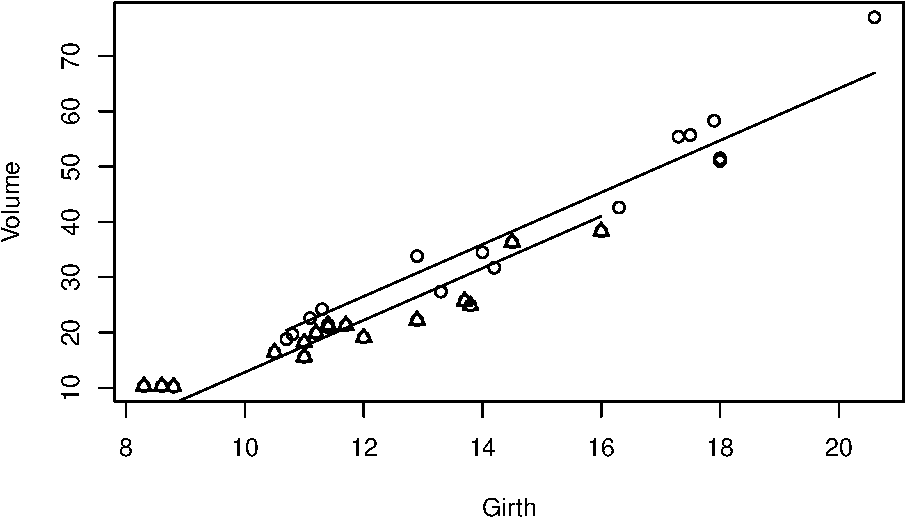
\includegraphics{_main_files/figure-latex/dummy-variable-trees-1.pdf}
\caption{\label{fig:dummy-variable-trees}\small A dummy variable model for the
\texttt{trees} data.}
\end{figure}




It may look intimidating but there is reason to the madness. First we
\texttt{split} the \texttt{trees} data into two pieces, with groups
determined by the \texttt{Tall} variable. Next we add the fitted values
to each piece via \texttt{predict}. Then we set up a \texttt{plot} for
the variables \texttt{Volume} versus \texttt{Girth}, but we do not plot
anything yet (\texttt{type\ =\ n}) because we want to use different
symbols for the two groups. Next we add \texttt{points} to the plot for
the \texttt{Tall\ =\ yes} trees and use an open circle for a plot
character (\texttt{pch\ =\ 1}), followed by \texttt{points} for the
\texttt{Tall\ =\ no} trees with a triangle character
(\texttt{pch\ =\ 2}). Finally, we add regression \texttt{lines} to the
plot, one for each group.

There are other -- shorter -- ways to plot regression lines by groups,
namely the \texttt{scatterplot} function in the \texttt{car} package
\autocite{car} and the \texttt{xyplot} function in the \texttt{lattice}
package \autocite{lattice}. We elected to introduce the reader to the
above approach since many advanced plots in R are done in a similar,
consecutive fashion.

\section{Partial F Statistic}\label{sec-partial-f-statistic}

We saw in Section \ref{sub-mlr-overall-f-test} how to test
\(H_{0}:\beta_{0}=\beta_{1}=\cdots=\beta_{p}=0\) with the overall \(F\)
statistic and we saw in Section \ref{sub-mlr-students-t-tests} how to
test \(H_{0}:\beta_{i}=0\) that a particular coefficient \(\beta_{i}\)
is zero. Sometimes, however, we would like to test whether a certain
part of the model is significant. Consider the regression model

\begin{equation}
Y=\beta_{0}+\beta_{1}x_{1}+\cdots+\beta_{j}x_{j}+\beta_{j+1}x_{j+1}+\cdots+\beta_{p}x_{p}+\epsilon,
\end{equation}

where \(j\geq1\) and \(p\geq2\). Now we wish to test the hypothesis

\begin{equation}
H_{0}:\beta_{j+1}=\beta_{j+2}=\cdots=\beta_{p}=0
\end{equation}

versus the alternative

\begin{equation}
H_{1}:\mbox{at least one of $\beta_{j+1},\ \beta_{j+2},\ ,\ldots,\beta_{p}\neq0$}.
\end{equation}

The interpretation of \(H_{0}\) is that none of the variables
\(x_{j+1}\), \ldots{},\(x_{p}\) is significantly related to \(Y\) and
the interpretation of \(H_{1}\) is that at least one of \(x_{j+1}\),
\ldots{},\(x_{p}\) is significantly related to \(Y\). In essence, for
this hypothesis test there are two competing models under consideration:

\begin{align}
\mbox{the full model:} & \quad y=\beta_{0}+\beta_{1}x_{1}+\cdots+\beta_{p}x_{p}+\epsilon,\\
\mbox{the reduced model:} & \quad y=\beta_{0}+\beta_{1}x_{1}+\cdots+\beta_{j}x_{j}+\epsilon,
\end{align}

Of course, the full model will always explain the data \emph{better}
than the reduced model, but does the full model explain the data
\emph{significantly better} than the reduced model? This question is
exactly what the partial \(F\) statistic is designed to answer.

We first calculate \(SSE_{f}\), the unexplained variation in the full
model, and \(SSE_{r}\), the unexplained variation in the reduced model.
We base our test on the difference \(SSE_{r}-SSE_{f}\) which measures
the reduction in unexplained variation attributable to the variables
\(x_{j+1}\), \ldots{}, \(x_{p}\). In the full model there are \(p+1\)
parameters and in the reduced model there are \(j+1\) parameters, which
gives a difference of \(p-j\) parameters (hence degrees of freedom). The
partial F statistic is

\begin{equation}
F=\frac{(SSE_{r}-SSE_{f})/(p-j)}{SSE_{f}/(n-p-1)}.
\end{equation}

It can be shown when the regression assumptions hold under \(H_{0}\)
that the partial \(F\) statistic has an
\(\mathsf{f}(\mathtt{df1}=p-j,\,\mathtt{df2}=n-p-1)\) distribution. We
calculate the \(p\)-value of the observed partial \(F\) statistic and
reject \(H_{0}\) if the \(p\)-value is small.

\subsection{How to do it with R}\label{how-to-do-it-with-r-44}

The key ingredient above is that the two competing models are
\emph{nested} in the sense that the reduced model is entirely contained
within the complete model. The way to test whether the improvement is
significant is to compute \texttt{lm} objects both for the complete
model and the reduced model then compare the answers with the
\texttt{anova} function.

\bigskip

\BeginKnitrBlock{example}[The Trees data]
\protect\hypertarget{ex:unnamed-chunk-328}{}{\label{ex:unnamed-chunk-328}
\iffalse (The Trees data) \fi }For the \texttt{trees} data, let us fit a
polynomial regression model and for the sake of argument we will ignore
our own good advice and fail to rescale the explanatory variables.
\EndKnitrBlock{example}

\begin{Shaded}
\begin{Highlighting}[]
\NormalTok{treesfull.lm <-}\StringTok{ }\KeywordTok{lm}\NormalTok{(Volume ~}\StringTok{ }\NormalTok{Girth +}\StringTok{ }\KeywordTok{I}\NormalTok{(Girth^}\DecValTok{2}\NormalTok{) +}\StringTok{ }\NormalTok{Height +}\StringTok{ }
\StringTok{                   }\KeywordTok{I}\NormalTok{(Height^}\DecValTok{2}\NormalTok{), }\DataTypeTok{data =} \NormalTok{trees)}
\KeywordTok{summary}\NormalTok{(treesfull.lm)}
\end{Highlighting}
\end{Shaded}

\begin{verbatim}

Call:
lm(formula = Volume ~ Girth + I(Girth^2) + Height + I(Height^2), 
    data = trees)

Residuals:
   Min     1Q Median     3Q    Max 
-4.368 -1.670 -0.158  1.792  4.358 

Coefficients:
             Estimate Std. Error t value Pr(>|t|)    
(Intercept) -0.955101  63.013630  -0.015    0.988    
Girth       -2.796569   1.468677  -1.904    0.068 .  
I(Girth^2)   0.265446   0.051689   5.135 2.35e-05 ***
Height       0.119372   1.784588   0.067    0.947    
I(Height^2)  0.001717   0.011905   0.144    0.886    
---
Signif. codes:  
0 '***' 0.001 '**' 0.01 '*' 0.05 '.' 0.1 ' ' 1

Residual standard error: 2.674 on 26 degrees of freedom
Multiple R-squared:  0.9771,    Adjusted R-squared:  0.9735 
F-statistic:   277 on 4 and 26 DF,  p-value: < 2.2e-16
\end{verbatim}

In this ill-formed model nothing is significant except \texttt{Girth}
and \texttt{Girth\^{}2}. Let us continue down this path and suppose that
we would like to try a reduced model which contains nothing but
\texttt{Girth} and \texttt{Girth\^{}2} (not even an \texttt{Intercept}).
Our two models are now

\begin{align*} 
\mbox{the full model:} & \quad Y=\beta_{0}+\beta_{1}x_{1}+\beta_{2}x_{1}^{2}+\beta_{3}x_{2}+\beta_{4}x_{2}^{2}+\epsilon,\\
\mbox{the reduced model:} & \quad Y=\beta_{1}x_{1}+\beta_{2}x_{1}^{2}+\epsilon,
\end{align*}

We fit the reduced model with \texttt{lm} and store the results:

\begin{Shaded}
\begin{Highlighting}[]
\NormalTok{treesreduced.lm <-}\StringTok{ }\KeywordTok{lm}\NormalTok{(Volume ~}\StringTok{ }\NormalTok{-}\DecValTok{1} \NormalTok{+}\StringTok{ }\NormalTok{Girth +}\StringTok{ }\KeywordTok{I}\NormalTok{(Girth^}\DecValTok{2}\NormalTok{), }\DataTypeTok{data =} \NormalTok{trees)}
\end{Highlighting}
\end{Shaded}

To delete the intercept from the model we used \texttt{-1} in the model
formula. Next we compare the two models with the \texttt{anova}
function. The convention is to list the models from smallest to largest.

\begin{Shaded}
\begin{Highlighting}[]
\KeywordTok{anova}\NormalTok{(treesreduced.lm, treesfull.lm)}
\end{Highlighting}
\end{Shaded}

\begin{verbatim}
Analysis of Variance Table

Model 1: Volume ~ -1 + Girth + I(Girth^2)
Model 2: Volume ~ Girth + I(Girth^2) + Height + I(Height^2)
  Res.Df    RSS Df Sum of Sq      F   Pr(>F)   
1     29 321.65                                
2     26 185.86  3    135.79 6.3319 0.002279 **
---
Signif. codes:  
0 '***' 0.001 '**' 0.01 '*' 0.05 '.' 0.1 ' ' 1
\end{verbatim}

We see from the output that the complete model is highly significant
compared to the model that does not incorporate \texttt{Height} or the
\texttt{Intercept}. We wonder (with our tongue in our cheek) if the
\texttt{Height\^{}2} term in the full model is causing all of the
trouble. We will fit an alternative reduced model that only deletes
\texttt{Height\^{}2}.

\begin{Shaded}
\begin{Highlighting}[]
\NormalTok{treesreduced2.lm <-}\StringTok{ }\KeywordTok{lm}\NormalTok{(Volume ~}\StringTok{ }\NormalTok{Girth +}\StringTok{ }\KeywordTok{I}\NormalTok{(Girth^}\DecValTok{2}\NormalTok{) +}\StringTok{ }\NormalTok{Height, }
                       \DataTypeTok{data =} \NormalTok{trees)}
\KeywordTok{anova}\NormalTok{(treesreduced2.lm, treesfull.lm)}
\end{Highlighting}
\end{Shaded}

\begin{verbatim}
Analysis of Variance Table

Model 1: Volume ~ Girth + I(Girth^2) + Height
Model 2: Volume ~ Girth + I(Girth^2) + Height + I(Height^2)
  Res.Df    RSS Df Sum of Sq      F Pr(>F)
1     27 186.01                           
2     26 185.86  1   0.14865 0.0208 0.8865
\end{verbatim}

In this case, the improvement to the reduced model that is attributable
to \texttt{Height\^{}2} is not significant, so we can delete
\texttt{Height\^{}2} from the model with a clear conscience. We notice
that the \emph{p}-value for this latest partial \(F\) test is 0.8865,
which seems to be remarkably close to the \emph{p}-value we saw for the
univariate \emph{t} test of \texttt{Height\^{}2} at the beginning of
this example. In fact, the \emph{p-values} are \emph{exactly} the same.
Perhaps now we gain some insight into the true meaning of the univariate
tests.

\section{Residual Analysis and Diagnostic
Tools}\label{sec-residual-analysis-mlr}

We encountered many, many diagnostic measures for simple linear
regression in Sections \ref{sec-residual-analysis-slr} and
\ref{sec-other-diagnostic-tools-slr}. All of these are valid in multiple
linear regression, too, but there are some slight changes that we need
to make for the multivariate case. We list these below, and apply them
to the trees example.

\begin{itemize}
\tightlist
\item
  \textbf{Shapiro-Wilk, Breusch-Pagan, Durbin-Watson:} unchanged from
  SLR, but we are now equipped to talk about the Shapiro-Wilk test
  statistic for the residuals. It is defined by the formula

  \begin{equation}
   W=\frac{\mathbf{a}^{\mathrm{T}}\mathbf{E}^{\ast}}{\mathbf{E}^{\mathrm{T}}\mathbf{E}},
   \end{equation}

  where \(\mathbf{E}^{\ast}\) is the sorted residuals and
  \(\mathbf{a}_{1\times\mathrm{n}}\) is defined by

  \begin{equation}
   \mathbf{a}=\frac{\mathbf{m}^{\mathrm{T}}\mathbf{V}^{-1}}{\sqrt{\mathbf{m}^{\mathrm{T}}\mathbf{V}^{-1}\mathbf{V}^{-1}\mathbf{m}}},
   \end{equation}

  where \(\mathbf{m}_{\mathrm{n}\times1}\) and
  \(\mathbf{V}_{\mathrm{n}\times\mathrm{n}}\) are the mean and
  covariance matrix, respectively, of the order statistics from an
  \(\mathsf{mvnorm}\left(\mathtt{mean}=\mathbf{0},\,\mathtt{sigma}=\mathbf{I}\right)\)
  distribution.
\item
  \textbf{Leverages:} are defined to be the diagonal entries of the hat
  matrix \(\mathbf{H}\) (which is why we called them \(h_{ii}\) in
  Section \ref{sub-mlr-point-est-regsurface}). The sum of the leverages
  is \(\mbox{tr}(\mathbf{H})=p+1\). One rule of thumb considers a
  leverage extreme if it is larger than double the mean leverage value,
  which is \(2(p+1)/n\), and another rule of thumb considers leverages
  bigger than 0.5 to indicate high leverage, while values between 0.3
  and 0.5 indicate moderate leverage.
\item
  \textbf{Standardized residuals:} unchanged. Considered extreme if
  \(|R_{i}|>2\).
\item
  \textbf{Studentized residuals:} compared to a
  \(\mathsf{t}(\mathtt{df}=n-p-2)\) distribution.
\item
  \textbf{DFBETAS:} The formula is generalized to

  \begin{equation}
     (DFBETAS)_{j(i)}=\frac{b_{j}-b_{j(i)}}{S_{(i)}\sqrt{c_{jj}}},\quad j=0,\ldots p,\ i=1,\ldots,n,
     \end{equation}

  where \(c_{jj}\) is the \(j^{\mathrm{th}}\) diagonal entry of
  \((\mathbf{X}^{\mathrm{T}}\mathbf{X})^{-1}\). Values larger than one
  for small data sets or \(2/\sqrt{n}\) for large data sets should be
  investigated.
\item
  \textbf{DFFITS:} unchanged. Larger than one in absolute value is
  considered extreme.
\item
  \textbf{Cook's D:} compared to an
  \(\mathsf{f}(\mathtt{df1} = p +  1,\,\mathtt{df2} = n - p - 1)\)
  distribution. Observations falling higher than the
  50\(^{\textrm{th}}\) percentile are extreme. Note that plugging the
  value \(p=1\) into the formulas will recover all of the ones we saw in
  Chapter \ref{cha-simple-linear-regression}.
\end{itemize}

\section{Additional Topics}\label{sec-additional-topics-mlr}

\subsection{Nonlinear Regression}\label{nonlinear-regression}

We spent the entire chapter talking about the \texttt{trees} data, and
all of our models looked like
\texttt{Volume\ \textasciitilde{}\ Girth\ +\ Height} or a variant of
this model. But let us think again: we know from elementary school that
the volume of a rectangle is \(V=lwh\) and the volume of a cylinder
(which is closer to what a black cherry tree looks like) is

\begin{equation}
V=\pi r^{2}h\quad \mbox{or}\quad V=4\pi dh,
\end{equation}

where \(r\) and \(d\) represent the radius and diameter of the tree,
respectively. With this in mind, it would seem that a more appropriate
model for \(\mu\) might be

\begin{equation}
\label{eq-trees-nonlin-reg}
\mu(x_{1},x_{2})=\beta_{0}x_{1}^{\beta_{1}}x_{2}^{\beta_{2}},
\end{equation}

where \(\beta_{1}\) and \(\beta_{2}\) are parameters to adjust for the
fact that a black cherry tree is not a perfect cylinder.

How can we fit this model? The model is not linear in the parameters any
more, so our linear regression methods will not work\ldots{} or will
they? In the \texttt{trees} example we may take the logarithm of both
sides of Equation \eqref{eq-trees-nonlin-reg} to get

\begin{equation}
\mu^{\ast}(x_{1},x_{2})=\ln\left[\mu(x_{1},x_{2})\right]=\ln\beta_{0}+\beta_{1}\ln x_{1}+\beta_{2}\ln x_{2},
\end{equation}

and this new model \(\mu^{\ast}\) is linear in the parameters
\(\beta_{0}^{\ast}=\ln\beta_{0}\), \(\beta_{1}^{\ast}=\beta_{1}\) and
\(\beta_{2}^{\ast}=\beta_{2}\). We can use what we have learned to fit a
linear model
\texttt{log(Volume)\ \textasciitilde{}\ log(Girth)\ +\ log(Height)}, and
everything will proceed as before, with one exception: we will need to
be mindful when it comes time to make predictions because the model will
have been fit on the log scale, and we will need to transform our
predictions back to the original scale (by exponentiating with
\texttt{exp}) to make sense.

\begin{Shaded}
\begin{Highlighting}[]
\NormalTok{treesNonlin.lm <-}\StringTok{ }\KeywordTok{lm}\NormalTok{(}\KeywordTok{log}\NormalTok{(Volume) ~}\StringTok{ }\KeywordTok{log}\NormalTok{(Girth) +}\StringTok{ }\KeywordTok{log}\NormalTok{(Height), }\DataTypeTok{data =} \NormalTok{trees)}
\KeywordTok{summary}\NormalTok{(treesNonlin.lm)}
\end{Highlighting}
\end{Shaded}

\begin{verbatim}

Call:
lm(formula = log(Volume) ~ log(Girth) + log(Height), data = trees)

Residuals:
      Min        1Q    Median        3Q       Max 
-0.168561 -0.048488  0.002431  0.063637  0.129223 

Coefficients:
            Estimate Std. Error t value Pr(>|t|)    
(Intercept) -6.63162    0.79979  -8.292 5.06e-09 ***
log(Girth)   1.98265    0.07501  26.432  < 2e-16 ***
log(Height)  1.11712    0.20444   5.464 7.81e-06 ***
---
Signif. codes:  
0 '***' 0.001 '**' 0.01 '*' 0.05 '.' 0.1 ' ' 1

Residual standard error: 0.08139 on 28 degrees of freedom
Multiple R-squared:  0.9777,    Adjusted R-squared:  0.9761 
F-statistic: 613.2 on 2 and 28 DF,  p-value: < 2.2e-16
\end{verbatim}

This is our best model yet (judging by \(R^{2}\) and
\(\overline{R}^{2}\)), all of the parameters are significant, it is
simpler than the quadratic or interaction models, and it even makes
theoretical sense. It rarely gets any better than that.

We may get confidence intervals for the parameters, but remember that it
is usually better to transform back to the original scale for
interpretation purposes:

\begin{Shaded}
\begin{Highlighting}[]
\KeywordTok{exp}\NormalTok{(}\KeywordTok{confint}\NormalTok{(treesNonlin.lm))}
\end{Highlighting}
\end{Shaded}

\begin{verbatim}
                   2.5 %      97.5 %
(Intercept) 0.0002561078 0.006783093
log(Girth)  6.2276411645 8.468066317
log(Height) 2.0104387829 4.645475188
\end{verbatim}

(Note that we did not update the row labels of the matrix to show that
we exponentiated and so they are misleading as written.) We do
predictions just as before. Remember to transform the response variable
back to the original scale after prediction.

\begin{Shaded}
\begin{Highlighting}[]
\NormalTok{new <-}\StringTok{ }\KeywordTok{data.frame}\NormalTok{(}\DataTypeTok{Girth =} \KeywordTok{c}\NormalTok{(}\FloatTok{9.1}\NormalTok{, }\FloatTok{11.6}\NormalTok{, }\FloatTok{12.5}\NormalTok{), }\DataTypeTok{Height =} \KeywordTok{c}\NormalTok{(}\DecValTok{69}\NormalTok{, }\DecValTok{74}\NormalTok{, }\DecValTok{87}\NormalTok{))}
\KeywordTok{exp}\NormalTok{(}\KeywordTok{predict}\NormalTok{(treesNonlin.lm, }\DataTypeTok{newdata =} \NormalTok{new, }\DataTypeTok{interval =} \StringTok{"confidence"}\NormalTok{))}
\end{Highlighting}
\end{Shaded}

\begin{verbatim}
       fit      lwr      upr
1 11.90117 11.25908 12.57989
2 20.82261 20.14652 21.52139
3 28.93317 27.03755 30.96169
\end{verbatim}

The predictions and intervals are slightly different from those
calculated earlier, but they are close. Note that we did not need to
transform the \texttt{Girth} and \texttt{Height} arguments in the
dataframe \texttt{new}. All transformations are done for us
automatically.

\subsection{Real Nonlinear Regression}\label{real-nonlinear-regression}

We saw with the \texttt{trees} data that a nonlinear model might be more
appropriate for the data based on theoretical considerations, and we
were lucky because the functional form of \(\mu\) allowed us to take
logarithms to transform the nonlinear model to a linear one. The same
trick will not work in other circumstances, however. We need techniques
to fit general models of the form

\begin{equation}
\mathbf{Y}=\mu(\mathbf{X})+\epsilon,
\end{equation}

where \(\mu\) is some crazy function that does not lend itself to linear
transformations.

There are a host of methods to address problems like these which are
studied in advanced regression classes. The interested reader should see
Neter \emph{et al} \autocite{Neter1996} or Tabachnick and Fidell
\autocite{Tabachnick2006}.

It turns out that John Fox has posted an Appendix to his book
\autocite{Fox2002} which discusses some of the methods and issues
associated with nonlinear regression; see
\url{http://cran.r-project.org/doc/contrib/Fox-Companion/appendix.html}
for more. Here is an example of how it works, based on a question from
R-help.

\begin{Shaded}
\begin{Highlighting}[]
\CommentTok{# fake data }
\KeywordTok{set.seed}\NormalTok{(}\DecValTok{1}\NormalTok{) }
\NormalTok{x <-}\StringTok{ }\KeywordTok{seq}\NormalTok{(}\DataTypeTok{from =} \DecValTok{0}\NormalTok{, }\DataTypeTok{to =} \DecValTok{1000}\NormalTok{, }\DataTypeTok{length.out =} \DecValTok{200}\NormalTok{) }
\NormalTok{y <-}\StringTok{ }\DecValTok{1} \NormalTok{+}\StringTok{ }\DecValTok{2}\NormalTok{*(}\KeywordTok{sin}\NormalTok{((}\DecValTok{2}\NormalTok{*pi*x/}\DecValTok{360}\NormalTok{) -}\StringTok{ }\DecValTok{3}\NormalTok{))^}\DecValTok{2} \NormalTok{+}\StringTok{ }\KeywordTok{rnorm}\NormalTok{(}\DecValTok{200}\NormalTok{, }\DataTypeTok{sd =} \DecValTok{2}\NormalTok{)}
\CommentTok{# plot(x, y)}
\NormalTok{acc.nls <-}\StringTok{ }\KeywordTok{nls}\NormalTok{(y ~}\StringTok{ }\NormalTok{a +}\StringTok{ }\NormalTok{b*(}\KeywordTok{sin}\NormalTok{((}\DecValTok{2}\NormalTok{*pi*x/}\DecValTok{360}\NormalTok{) -}\StringTok{ }\NormalTok{c))^}\DecValTok{2}\NormalTok{, }
               \DataTypeTok{start =} \KeywordTok{list}\NormalTok{(}\DataTypeTok{a =} \FloatTok{0.9}\NormalTok{, }\DataTypeTok{b =} \FloatTok{2.3}\NormalTok{, }\DataTypeTok{c =} \FloatTok{2.9}\NormalTok{))}
\KeywordTok{summary}\NormalTok{(acc.nls)}
\end{Highlighting}
\end{Shaded}

\begin{verbatim}

Formula: y ~ a + b * (sin((2 * pi * x/360) - c))^2

Parameters:
  Estimate Std. Error t value Pr(>|t|)    
a  0.95884    0.23097   4.151 4.92e-05 ***
b  2.22868    0.37114   6.005 9.07e-09 ***
c  3.04343    0.08434  36.084  < 2e-16 ***
---
Signif. codes:  
0 '***' 0.001 '**' 0.01 '*' 0.05 '.' 0.1 ' ' 1

Residual standard error: 1.865 on 197 degrees of freedom

Number of iterations to convergence: 3 
Achieved convergence tolerance: 6.407e-08
\end{verbatim}

\begin{Shaded}
\begin{Highlighting}[]
\CommentTok{#plot(x, fitted(acc.nls))}
\end{Highlighting}
\end{Shaded}

\subsection{Multicollinearity}\label{sub-multicollinearity}

A multiple regression model exhibits \emph{multicollinearity} when two
or more of the explanatory variables are substantially correlated with
each other. We can measure multicollinearity by having one of the
explanatory play the role of ``dependent variable'' and regress it on
the remaining explanatory variables. The the \(R^{2}\) of the resulting
model is near one, then we say that the model is multicollinear or shows
multicollinearity.

Multicollinearity is a problem because it causes instability in the
regression model. The instability is a consequence of redundancy in the
explanatory variables: a high \(R^{2}\) indicates a strong dependence
between the selected independent variable and the others. The redundant
information inflates the variance of the parameter estimates which can
cause them to be statistically insignificant when they would have been
significant otherwise. To wit, multicollinearity is usually measured by
what are called \emph{variance inflation factors}.

Once multicollinearity has been diagnosed there are several approaches
to remediate it. Here are a couple of important ones.

\begin{itemize}
\tightlist
\item
  \textbf{Principal Components Analysis.} This approach casts out two or
  more of the original explanatory variables and replaces them with new
  variables, derived from the original ones, that are by design
  uncorrelated with one another. The redundancy is thus eliminated and
  we may proceed as usual with the new variables in hand. Principal
  Components Analysis is important for other reasons, too, not just for
  fixing multicollinearity problems.
\item
  \textbf{Ridge Regression.} The idea of this approach is to replace the
  original parameter estimates with a different type of parameter
  estimate which is more stable under multicollinearity. The estimators
  are not found by ordinary least squares but rather a different
  optimization procedure which incorporates the variance inflation
  factor information.
\end{itemize}

We decided to omit a thorough discussion of multicollinearity because we
are not equipped to handle the mathematical details. Perhaps the topic
will receive more attention in a later edition.

\begin{itemize}
\tightlist
\item
  What to do when data are not normal
\item
  Bootstrap (see Chapter \ref{cha-resampling-methods}).
\end{itemize}

\subsection{Akaike's Information
Criterion}\label{akaikes-information-criterion}

\[
AIC = -2\ln L + 2(p + 1)
\]

\section{Exercises}\label{exercises-5}

\textbf{Exercise.} Use Equations \eqref{eq-mlr-sse-matrix},
\eqref{eq-mlr-ssto-matrix}, and \eqref{eq-mlr-ssr-matrix} to prove the
Anova Equality: \[ SSTO = SSE + SSR.\]

\printbibliography

\cleardoublepage
\phantomsection
\addcontentsline{toc}{chapter}{\bibname}
%\bibliographystyle{plainurl}
\nocite{*}
%\bibliography{IPSUR,Rpackages}
\vfill{}
\cleardoublepage
\phantomsection
\addcontentsline{toc}{chapter}{\indexname} 
\printindex{}


\end{document}
